% Options for packages loaded elsewhere
\PassOptionsToPackage{unicode}{hyperref}
\PassOptionsToPackage{hyphens}{url}
%
\documentclass[
  12pt,
]{book}
\usepackage{amsmath,amssymb}
\usepackage{lmodern}
\usepackage{setspace}
\usepackage{ifxetex,ifluatex}
\ifnum 0\ifxetex 1\fi\ifluatex 1\fi=0 % if pdftex
  \usepackage[T1]{fontenc}
  \usepackage[utf8]{inputenc}
  \usepackage{textcomp} % provide euro and other symbols
\else % if luatex or xetex
  \usepackage{unicode-math}
  \defaultfontfeatures{Scale=MatchLowercase}
  \defaultfontfeatures[\rmfamily]{Ligatures=TeX,Scale=1}
\fi
% Use upquote if available, for straight quotes in verbatim environments
\IfFileExists{upquote.sty}{\usepackage{upquote}}{}
\IfFileExists{microtype.sty}{% use microtype if available
  \usepackage[]{microtype}
  \UseMicrotypeSet[protrusion]{basicmath} % disable protrusion for tt fonts
}{}
\makeatletter
\@ifundefined{KOMAClassName}{% if non-KOMA class
  \IfFileExists{parskip.sty}{%
    \usepackage{parskip}
  }{% else
    \setlength{\parindent}{0pt}
    \setlength{\parskip}{6pt plus 2pt minus 1pt}}
}{% if KOMA class
  \KOMAoptions{parskip=half}}
\makeatother
\usepackage{xcolor}
\IfFileExists{xurl.sty}{\usepackage{xurl}}{} % add URL line breaks if available
\IfFileExists{bookmark.sty}{\usepackage{bookmark}}{\usepackage{hyperref}}
\hypersetup{
  pdftitle={Estudio Longitudinal Social de Chile},
  hidelinks,
  pdfcreator={LaTeX via pandoc}}
\urlstyle{same} % disable monospaced font for URLs
\usepackage[left=4cm, right=3cm, top=2.5cm, bottom=2.5cm]{geometry}
\usepackage{color}
\usepackage{fancyvrb}
\newcommand{\VerbBar}{|}
\newcommand{\VERB}{\Verb[commandchars=\\\{\}]}
\DefineVerbatimEnvironment{Highlighting}{Verbatim}{commandchars=\\\{\}}
% Add ',fontsize=\small' for more characters per line
\usepackage{framed}
\definecolor{shadecolor}{RGB}{248,248,248}
\newenvironment{Shaded}{\begin{snugshade}}{\end{snugshade}}
\newcommand{\AlertTok}[1]{\textcolor[rgb]{0.94,0.16,0.16}{#1}}
\newcommand{\AnnotationTok}[1]{\textcolor[rgb]{0.56,0.35,0.01}{\textbf{\textit{#1}}}}
\newcommand{\AttributeTok}[1]{\textcolor[rgb]{0.77,0.63,0.00}{#1}}
\newcommand{\BaseNTok}[1]{\textcolor[rgb]{0.00,0.00,0.81}{#1}}
\newcommand{\BuiltInTok}[1]{#1}
\newcommand{\CharTok}[1]{\textcolor[rgb]{0.31,0.60,0.02}{#1}}
\newcommand{\CommentTok}[1]{\textcolor[rgb]{0.56,0.35,0.01}{\textit{#1}}}
\newcommand{\CommentVarTok}[1]{\textcolor[rgb]{0.56,0.35,0.01}{\textbf{\textit{#1}}}}
\newcommand{\ConstantTok}[1]{\textcolor[rgb]{0.00,0.00,0.00}{#1}}
\newcommand{\ControlFlowTok}[1]{\textcolor[rgb]{0.13,0.29,0.53}{\textbf{#1}}}
\newcommand{\DataTypeTok}[1]{\textcolor[rgb]{0.13,0.29,0.53}{#1}}
\newcommand{\DecValTok}[1]{\textcolor[rgb]{0.00,0.00,0.81}{#1}}
\newcommand{\DocumentationTok}[1]{\textcolor[rgb]{0.56,0.35,0.01}{\textbf{\textit{#1}}}}
\newcommand{\ErrorTok}[1]{\textcolor[rgb]{0.64,0.00,0.00}{\textbf{#1}}}
\newcommand{\ExtensionTok}[1]{#1}
\newcommand{\FloatTok}[1]{\textcolor[rgb]{0.00,0.00,0.81}{#1}}
\newcommand{\FunctionTok}[1]{\textcolor[rgb]{0.00,0.00,0.00}{#1}}
\newcommand{\ImportTok}[1]{#1}
\newcommand{\InformationTok}[1]{\textcolor[rgb]{0.56,0.35,0.01}{\textbf{\textit{#1}}}}
\newcommand{\KeywordTok}[1]{\textcolor[rgb]{0.13,0.29,0.53}{\textbf{#1}}}
\newcommand{\NormalTok}[1]{#1}
\newcommand{\OperatorTok}[1]{\textcolor[rgb]{0.81,0.36,0.00}{\textbf{#1}}}
\newcommand{\OtherTok}[1]{\textcolor[rgb]{0.56,0.35,0.01}{#1}}
\newcommand{\PreprocessorTok}[1]{\textcolor[rgb]{0.56,0.35,0.01}{\textit{#1}}}
\newcommand{\RegionMarkerTok}[1]{#1}
\newcommand{\SpecialCharTok}[1]{\textcolor[rgb]{0.00,0.00,0.00}{#1}}
\newcommand{\SpecialStringTok}[1]{\textcolor[rgb]{0.31,0.60,0.02}{#1}}
\newcommand{\StringTok}[1]{\textcolor[rgb]{0.31,0.60,0.02}{#1}}
\newcommand{\VariableTok}[1]{\textcolor[rgb]{0.00,0.00,0.00}{#1}}
\newcommand{\VerbatimStringTok}[1]{\textcolor[rgb]{0.31,0.60,0.02}{#1}}
\newcommand{\WarningTok}[1]{\textcolor[rgb]{0.56,0.35,0.01}{\textbf{\textit{#1}}}}
\usepackage{longtable,booktabs,array}
\usepackage{calc} % for calculating minipage widths
% Correct order of tables after \paragraph or \subparagraph
\usepackage{etoolbox}
\makeatletter
\patchcmd\longtable{\par}{\if@noskipsec\mbox{}\fi\par}{}{}
\makeatother
% Allow footnotes in longtable head/foot
\IfFileExists{footnotehyper.sty}{\usepackage{footnotehyper}}{\usepackage{footnote}}
\makesavenoteenv{longtable}
\usepackage{graphicx}
\makeatletter
\def\maxwidth{\ifdim\Gin@nat@width>\linewidth\linewidth\else\Gin@nat@width\fi}
\def\maxheight{\ifdim\Gin@nat@height>\textheight\textheight\else\Gin@nat@height\fi}
\makeatother
% Scale images if necessary, so that they will not overflow the page
% margins by default, and it is still possible to overwrite the defaults
% using explicit options in \includegraphics[width, height, ...]{}
\setkeys{Gin}{width=\maxwidth,height=\maxheight,keepaspectratio}
% Set default figure placement to htbp
\makeatletter
\def\fps@figure{htbp}
\makeatother
\setlength{\emergencystretch}{3em} % prevent overfull lines
\providecommand{\tightlist}{%
  \setlength{\itemsep}{0pt}\setlength{\parskip}{0pt}}
\setcounter{secnumdepth}{5}
\ifluatex
  \usepackage{selnolig}  % disable illegal ligatures
\fi

\title{Estudio Longitudinal Social de Chile}
\usepackage{etoolbox}
\makeatletter
\providecommand{\subtitle}[1]{% add subtitle to \maketitle
  \apptocmd{\@title}{\par {\large #1 \par}}{}{}
}
\makeatother
\subtitle{Resultados longitudinales 2016-2021}
\author{}
\date{\vspace{-2.5em}2021-10-06}

\begin{document}
\maketitle

{
\setcounter{tocdepth}{1}
\tableofcontents
}
\listoftables
\listoffigures
\setstretch{1.5}
\begin{Shaded}
\begin{Highlighting}[]
\FunctionTok{remove}\NormalTok{(}\AttributeTok{list =} \FunctionTok{ls}\NormalTok{())}

\CommentTok{\# bases de datos ELSOC}
\NormalTok{elsoc}\SpecialCharTok{::}\FunctionTok{load\_elsoc}\NormalTok{(}\AttributeTok{format =} \StringTok{\textquotesingle{}long\textquotesingle{}}\NormalTok{)}
\NormalTok{elsoc}\SpecialCharTok{::}\FunctionTok{load\_elsoc}\NormalTok{(}\AttributeTok{format =} \StringTok{\textquotesingle{}wide\textquotesingle{}}\NormalTok{)}
\end{Highlighting}
\end{Shaded}

\begin{Shaded}
\begin{Highlighting}[]
\CommentTok{\# Datos de dias de cuarentena por comuna de Ministerio de Ciencia:}

\CommentTok{\# Url para descarga directa de datos desde el Github del Ministerio de Ciencia}
\NormalTok{url }\OtherTok{\textless{}{-}} \StringTok{"https://raw.githubusercontent.com/MinCiencia/Datos{-}COVID19/master/output"}

\DocumentationTok{\#\# Cuarentenas desde 2020/03 hasta 2020/07/28 }
\NormalTok{cuarentenas1\_bruto }\OtherTok{\textless{}{-}} \FunctionTok{read\_csv}\NormalTok{(}\FunctionTok{paste}\NormalTok{(url, }\StringTok{"producto29"}\NormalTok{, }\StringTok{"Cuarentenas{-}Totales.csv"}\NormalTok{, }\AttributeTok{sep=}\StringTok{"/"}\NormalTok{))}

\NormalTok{cuarentenas1 }\OtherTok{\textless{}{-}}\NormalTok{ cuarentenas1\_bruto }\SpecialCharTok{\%\textgreater{}\%} 
\NormalTok{  janitor}\SpecialCharTok{::}\FunctionTok{clean\_names}\NormalTok{() }\SpecialCharTok{\%\textgreater{}\%} 
  \FunctionTok{mutate}\NormalTok{(}\AttributeTok{fecha\_de\_inicio =} \FunctionTok{as\_date}\NormalTok{(fecha\_de\_inicio),}
         \AttributeTok{fecha\_de\_termino =} \FunctionTok{as\_date}\NormalTok{(fecha\_de\_termino),}
         \CommentTok{\# cortar en fecha 2020/07/27 }
         \AttributeTok{fecha\_de\_termino =} \FunctionTok{as\_date}\NormalTok{(}\FunctionTok{ifelse}\NormalTok{(fecha\_de\_termino }\SpecialCharTok{\textgreater{}} \StringTok{\textquotesingle{}2020/07/27\textquotesingle{}}\NormalTok{, }
                                           \FunctionTok{make\_date}\NormalTok{(}\DecValTok{2020}\NormalTok{, }\DecValTok{07}\NormalTok{, }\DecValTok{27}\NormalTok{),}
\NormalTok{                                           fecha\_de\_termino)),}
         \AttributeTok{csum1 =} \FunctionTok{as.numeric}\NormalTok{(fecha\_de\_termino }\SpecialCharTok{{-}}\NormalTok{ fecha\_de\_inicio, }\AttributeTok{units =} \StringTok{\textquotesingle{}days\textquotesingle{}}\NormalTok{)) }\SpecialCharTok{\%\textgreater{}\%} 
  \FunctionTok{filter}\NormalTok{(fecha\_de\_inicio }\SpecialCharTok{\textless{}} \StringTok{\textquotesingle{}2020/07/27\textquotesingle{}}\NormalTok{) }\SpecialCharTok{\%\textgreater{}\%} 
  \FunctionTok{rename}\NormalTok{(}\AttributeTok{comuna\_cod =}\NormalTok{ codigo\_cut\_comuna) }\SpecialCharTok{\%\textgreater{}\%}
  \FunctionTok{group\_by}\NormalTok{(comuna\_cod) }\SpecialCharTok{\%\textgreater{}\%} 
  \FunctionTok{summarise}\NormalTok{(}\AttributeTok{csum1 =} \FunctionTok{mean}\NormalTok{(csum1, }\AttributeTok{na.rm =} \ConstantTok{TRUE}\NormalTok{)) }\SpecialCharTok{\%\textgreater{}\%} 
  \FunctionTok{ungroup}\NormalTok{()}

\DocumentationTok{\#\# Cuarentenas desde 2020/07/28 al último día actualizado}
\NormalTok{cuarentenas2\_bruto }\OtherTok{\textless{}{-}} \FunctionTok{read\_csv}\NormalTok{(}\FunctionTok{paste}\NormalTok{(url, }\StringTok{\textquotesingle{}producto74\textquotesingle{}}\NormalTok{, }\StringTok{"paso\_a\_paso\_std.csv"}\NormalTok{, }\AttributeTok{sep=}\StringTok{"/"}\NormalTok{))}

\NormalTok{cuarentenas2 }\OtherTok{\textless{}{-}}\NormalTok{ cuarentenas2\_bruto }\SpecialCharTok{\%\textgreater{}\%} 
\NormalTok{  janitor}\SpecialCharTok{::}\FunctionTok{clean\_names}\NormalTok{() }\SpecialCharTok{\%\textgreater{}\%} 
  \FunctionTok{mutate}\NormalTok{(}\AttributeTok{fecha =} \FunctionTok{as\_date}\NormalTok{(fecha),}
         \AttributeTok{dia =} \FunctionTok{weekdays}\NormalTok{(fecha),}
         \AttributeTok{cuarentena =} \FunctionTok{case\_when}\NormalTok{(paso}\SpecialCharTok{==}\DecValTok{1} \SpecialCharTok{\textasciitilde{}} \DecValTok{1}\NormalTok{,}
\NormalTok{                                paso}\SpecialCharTok{==}\DecValTok{2} \SpecialCharTok{\&}\NormalTok{ dia }\SpecialCharTok{\%in\%} \FunctionTok{c}\NormalTok{(}\StringTok{\textquotesingle{}Saturday\textquotesingle{}}\NormalTok{, }\StringTok{\textquotesingle{}Sunday\textquotesingle{}}\NormalTok{) }\SpecialCharTok{\textasciitilde{}} \DecValTok{1}\NormalTok{,}
                                \ConstantTok{TRUE} \SpecialCharTok{\textasciitilde{}} \DecValTok{0}\NormalTok{)) }\SpecialCharTok{\%\textgreater{}\%} 
  \FunctionTok{filter}\NormalTok{(zona }\SpecialCharTok{\%in\%} \FunctionTok{c}\NormalTok{(}\StringTok{\textquotesingle{}Urbana\textquotesingle{}}\NormalTok{, }\StringTok{\textquotesingle{}Total\textquotesingle{}}\NormalTok{)) }\SpecialCharTok{\%\textgreater{}\%} 
  \CommentTok{\# Días de cuarentena acumuladas desde el 2020/07/27 a la fecha de entrevista:}
  \FunctionTok{group\_by}\NormalTok{(codigo\_comuna, zona) }\SpecialCharTok{\%\textgreater{}\%} 
  \FunctionTok{mutate}\NormalTok{(}\AttributeTok{csum2 =} \FunctionTok{cumsum}\NormalTok{(cuarentena),}
         \AttributeTok{comuna\_cod =} \FunctionTok{as.numeric}\NormalTok{(codigo\_comuna)) }\SpecialCharTok{\%\textgreater{}\%} 
  \FunctionTok{ungroup}\NormalTok{() }\SpecialCharTok{\%\textgreater{}\%} 
  \FunctionTok{select}\NormalTok{(fecha, comuna\_cod, csum2)}

\CommentTok{\# Unir fechas:}
\NormalTok{cuarentenas\_acum }\OtherTok{\textless{}{-}} \FunctionTok{full\_join}\NormalTok{(cuarentenas1,}
\NormalTok{                              cuarentenas2,}
                              \AttributeTok{by =} \StringTok{\textquotesingle{}comuna\_cod\textquotesingle{}}\NormalTok{) }\SpecialCharTok{\%\textgreater{}\%} 
  \FunctionTok{rowwise}\NormalTok{() }\SpecialCharTok{\%\textgreater{}\%} 
  \FunctionTok{mutate}\NormalTok{(}\AttributeTok{dias\_cuarentena =} \FunctionTok{sum}\NormalTok{(csum1, csum2, }\AttributeTok{na.rm =} \ConstantTok{TRUE}\NormalTok{)) }\SpecialCharTok{\%\textgreater{}\%} 
  \FunctionTok{ungroup}\NormalTok{() }\SpecialCharTok{\%\textgreater{}\%} 
  \FunctionTok{mutate}\NormalTok{(}\AttributeTok{dias\_cuarentena\_t =} \FunctionTok{factor}\NormalTok{(car}\SpecialCharTok{::}\FunctionTok{recode}\NormalTok{(dias\_cuarentena, }\StringTok{\textquotesingle{}0 = 1; 1:50 = 2; 51:100 = 3; 101:999 = 4\textquotesingle{}}\NormalTok{),}
                                    \AttributeTok{levels =} \DecValTok{1}\SpecialCharTok{:}\DecValTok{4}\NormalTok{,}
                                    \AttributeTok{labels =} \FunctionTok{c}\NormalTok{(}\StringTok{\textquotesingle{}0 días\textquotesingle{}}\NormalTok{, }\StringTok{\textquotesingle{}1{-}50 días\textquotesingle{}}\NormalTok{, }\StringTok{\textquotesingle{}51{-}100 días\textquotesingle{}}\NormalTok{, }\StringTok{\textquotesingle{}Más de 100 días\textquotesingle{}}\NormalTok{))) }
\end{Highlighting}
\end{Shaded}

\hypertarget{introducciuxf3n}{%
\chapter{Introducción}\label{introducciuxf3n}}

El Centro de Estudios de Conflicto y Cohesión Social (COES) tiene el agrado de publicar el informe ``Radiografía del Cambio Social,'' el cual consolida los principales hallazgos longitudinales de cinco mediciones anuales del Estudio Longitudinal Social de Chile (ELSOC 2016-2021).

ELSOC es una encuesta desarrollada para analizar longitudinalmente, en un estudio panel, la evolución del conflicto y cohesión social en la sociedad chilena, basándose en modelos conceptuales descritos en la literatura nacional e internacional de las disciplinas del ámbito de la Economía, Sociología, Psicología, Ciencia Política y Estudios Urbanos. De este modo, se orienta a examinar los principales antecedentes, factores moderadores y mediadores, así como las principales consecuencias asociadas al desarrollo de distintas formas de sociabilidad en Chile.

Desde 2019 y hasta la fecha, Chile se ha visto remecido por importantes eventos que han alterado aspectos sociales, políticos y económicos de la vida nacional: la pandemia asociada al COVID-19, y las consecuencias del estallido social más grande de las últimas décadas, ocurrido a partir de octubre de 2019, el que ha desencadenado un proceso constituyente inédito en la historia de Chile.

Ambos fenómenos han significado un desafío para ELSOC, ya que afecta tanto la forma en que son levantados los datos, como las preguntas que el estudio debe abordar. Sin embargo, ELSOC presente una gran oportunidad única: la posibilidad de observar el efecto que éstos fenómenos tienen sobre la población chilena desde una perspectiva longitudinal.

\hypertarget{sobre-coes}{%
\section{Sobre COES}\label{sobre-coes}}

El Centro de Estudios de Conflicto y Cohesión Social (COES) desarrolla investigación colaborativa en temas relacionados al conflicto social y la cohesión (convivencia) en Chile, por medio de un equipo multidisciplinario proveniente de las ciencias sociales y humanidades. COES centra sus actividades académicas y de difusión en el análisis de las múltiples manifestaciones del conflicto y cohesión social en Chile, sus causas, así como también su contexto cultural e histórico.

COES está patrocinado por la Universidad de Chile y la Pontificia Universidad Católica de Chile, y como instituciones asociadas se encuentran la Universidad Diego Portales y la Universidad Adolfo Ibáñez. COES cuenta con el apoyo del Fondo de Financiamiento de Centros de Investigación en Áreas Prioritarias (FONDAP, dependiente de la Agencia Nacional de Investigación y Desarrollo (ANID) del Ministerio de Ciencia, Tecnología, Conocimiento e Innovación. ELSOC además cuenta como socio al Instituto Milenio para la Investigación en Depresión y Personalidad (MIDAP).

\hypertarget{sobre-elsoc}{%
\chapter{Sobre ELSOC}\label{sobre-elsoc}}

\hypertarget{descripciuxf3n-del-estudio}{%
\section{Descripción del estudio}\label{descripciuxf3n-del-estudio}}

El Estudio Longitudinal Social de Chile (ELSOC) es una encuesta panel, representativa de la población nacional urbana, que analiza la estabilidad y cambio de las creencias, actitudes y percepciones que tenemos los chilenos y chilenas respecto de la convivencia y del conflicto, la cohesión y una amplia gama de aspectos políticos y sociales a lo largo del tiempo.

Este estudio sigue la evolución de cerca de 4.500 chilenos y chilenas a lo largo de una década. Actualmente se encuentran disponibles 5 olas del estudio, abarcando el período entre 2016 y 2021. Sus temas de estudio y su aspecto longitudinal convierten a ELSOC en un recurso único en Chile y América Latina para analizar la evolución de la sociedad chilena y para el desarrollo de las ciencias sociales en Chile.

Durante los últimos años, ELSOC se ha consolidado como un importante insumo para el desarrollo de investigación científica y aplicada en ciencias sociales. En el sitio web \url{http://elsoc.cl} se puede acceder a más información sobre el estudio.

\hypertarget{acceso-a-bases-de-datos-elsoc}{%
\section{Acceso a Bases de Datos ELSOC}\label{acceso-a-bases-de-datos-elsoc}}

Las bases de datos y documentación correspondientes se encuentran disponibles, de manera libre y gratuita, en un repositorio de datos, al cual se podrá acceder en el link:

\url{https://dataverse.harvard.edu/dataverse/elsoc}

En este link se obtendrá acceso a los datos de las 5 mediciones transversales de ELSOC, así como bases longitudinales que integran las distintas mediciones. En colaboración con el Centro de Inteligencia Territorial (CIT), se pone también a disposición las bases ELSOC-CIT. Estas bases de datos permiten combinar la información de ELSOC, y estimaciones e indicadores territoriales y geoespaciales de distinta índole, proveniente de diversas fuentes de información nacional para los períodos 2016 a 2019.

ELSOC tiene un compromiso con los más altos estándares científicos en términos de producción y análisis de datos. Dentro de esta visión global, ELSOC se guía por las principales pautas de Transparencia y Apertura en la investigación científica. Por esta misma razón, los códigos utilizados para el desarrollo de este documento se encontrarán disponibles en \url{https://github.com/centro-coes}.

\hypertarget{caracteruxedsticas-del-diseuxf1o-muestral}{%
\section{Características del diseño muestral}\label{caracteruxedsticas-del-diseuxf1o-muestral}}

\begin{itemize}
\item
  Unidad de Análisis: Individuos
\item
  Muestra objetivo: 3.000 individuos en muestra original (a partir de 2016) y 1.500 en muestra refresco (a partir de 2018)
\item
  Población Objetivo: Hombres y mujeres de 18 a 75 años, residentes habituales de viviendas particulares ocupadas en zonas urbanas, localizadas en 40 ciudades (92 comunas, 13 regiones) del país
\item
  Periodicidad: Anual.
\end{itemize}

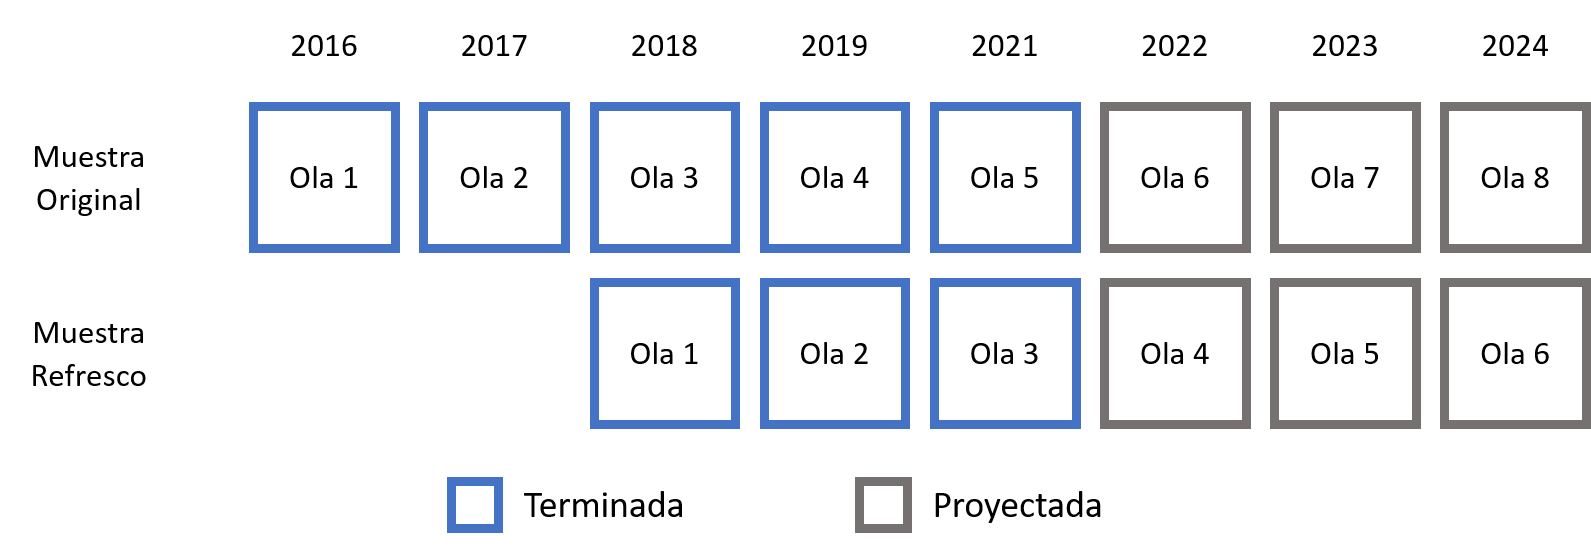
\includegraphics[width=22.1in]{1_input/imagenes/olas_elsoc}

\begin{itemize}
\item
  Marco Muestral: Marco de muestreo de manzanas del pre-censo 2011
\item
  Diseño Muestral: Probabilístico, estratificado (por tamaño de ciudades), por conglomerados y multietápico
\item
  Unidades de Muestreo: Primero se eligen ciudades (UPM), luego manzanas (USM), y sub-bloques y viviendas (UTM). La unidad final de selección es la persona
\end{itemize}

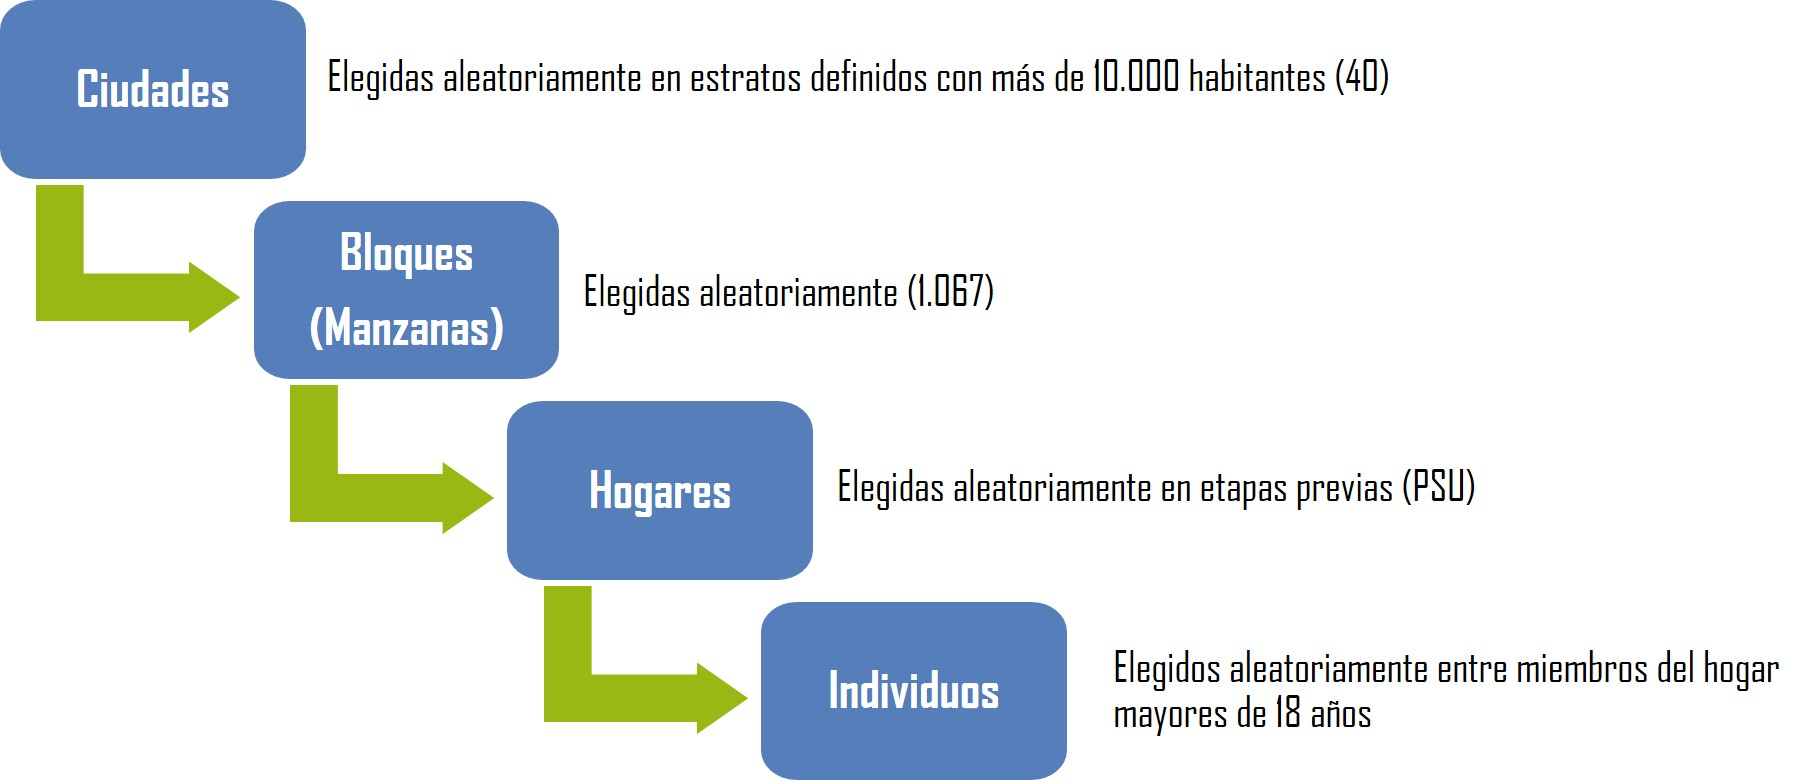
\includegraphics[width=25.24in]{1_input/imagenes/etapas_seleccion}

\textbf{Organismo Ejecutor}: Consultora Stephanie Eckman y Centro de Inteligencia Territorial (CIT) de la Universidad Adolfo Ibáñez

\hypertarget{caracteruxedsticas-del-levantamiento-de-datos}{%
\section{Características del levantamiento de datos}\label{caracteruxedsticas-del-levantamiento-de-datos}}

\begin{itemize}
\item
  Formato de aplicación: Cuestionario estructurado. Levantamiento en formato CAPI (Encuesta presencial con asistencia de tablet). Excepcionalmente se cambió a formato CATI (Encuesta telefónica con asistencia de tablet) durante 2021, debido a contingencia COVID-19
\item
  Período de Aplicación: entre Julio y Noviembre de cada año. Debido al estallido social, la cuarta medición se aplicó entre el 21 de noviembre de 2019 y el 9 de marzo de 2020. Debido a la pandemia, la quinta medición se aplicó entre el 29 de enero de 2021 y 12 de julio de 2021
\item
  Instrumento: Cuestionario compuesto por preguntas cerradas de carácter simple y múltiple junto a algunas preguntas abiertas. Combina módulos de preguntas permanentes (medidas en todas las olas) y otras intercaladas entre olas
\item
  Cobertura Temática: Contiene siete módulos temáticos: Territorio, Redes y actitudes sociales, Ciudadanía y democracia, Desigualdad y legitimidad, Conflicto social, Salud y bienestar y Caracterización sociodemográfica
\item
  Incentivos a la participación: Entrega de incentivos monetarios para el encuestado (\$ 6.000 CLP) y de material sobre el estudio (ELSOC y COES). Acciones de seguimiento basadas en la información de contacto (correo electrónico para cumpleaños y días festivos)
\item
  Entrenamiento de entrevistadores: Contratación de entrevistadores con experiencia en encuestas complejas y/o longitudinales. Capacitación centralizada y presencial para coordinadores de campo y un subconjunto de entrevistadores en Santiago (incluidos ejercicios prácticos para la implementación del cuestionario, uso de tabletas y protocolo de contacto). Actividades adicionales en otras regiones de Chile. Diseño de un Manual de entrevistador especializado para el proyecto
\item
  Operaciones de Control y Supervisión: Coordinadores de campo supervisan el trabajo de entrevistadores, verificando el número de visitas, el contacto, la identidad del participante y preguntas claves. Organismo ejecutor realiza una supervisión interna de al menos el 10\% de la muestra (entrevistando nuevamente a algunos encuestados), verificando la duración y la respuesta de los participantes
\end{itemize}

\textbf{Organismo Ejecutor}: Levantamiento a cargo de Centro Micro Datos (CMD) de la Universidad de Chile

\hypertarget{atriciuxf3n-de-la-muestra}{%
\chapter{Atrición de la muestra}\label{atriciuxf3n-de-la-muestra}}

El diseño de ELSOC contempló entrevistar a 3.000 personas en su muestra original y 1.500 en la muestra refresco. Sin embargo, es habitual que en encuestas panel se reduce el número de participantes, dado que algunos optan voluntariamente por dejar de participar y otras personas no pueden ser recontactadas. Este fenómeno es conocido como atrición, y pueden tener efectos nocivos sobre la utilidad de los datos longitudinales. En el caso de ELSOC, la tasa de atrición es comparativamente baja en comparación a otros estudios similares, por lo que no se considera al momento un problema significativo. A pesar de esto, el año 2018 se introduce una muestra refresco para contraarrestar el efecto de la atrición.

El año 2021, la atrición presenta un alza importante debido a la mayor dificultad que implica el levantamiento durante la pandemia de COVID-19 y al cambio de modalidad.

\begin{table}[H]
\centering\begin{table}[H]
\centering
\begin{tabular}[t]{c|c|c|c|c}
\hline
\multicolumn{1}{c|}{ } & \multicolumn{2}{c|}{Muestra original} & \multicolumn{2}{c}{Muestra refresco} \\
\cline{2-3} \cline{4-5}
Medición & Muestra lograda & Atrición & Muestra lograda & Atrición\\
\hline
2016 & 2 927 &  &  & \\
\hline
2017 & 2 473 & 15.5\% &  & \\
\hline
2018 & 2 229 & 9.9\% & 1 519 & \\
\hline
2019 & 2 153 & 3.4\% & 1 264 & 16.8\%\\
\hline
2021 & 1 739 & 19.2\% & 1 001 & 20.8\%\\
\hline
\end{tabular}
\end{table}
\end{table}

\hypertarget{foco-en-el-cambio-individual}{%
\chapter{Foco en el cambio individual}\label{foco-en-el-cambio-individual}}

Radiografía del Cambio Social tiene como objetivo fundamental caracterizar la estabilidad y el cambio en opiniones, actitudes y conductas de los participantes a lo largo del tiempo, enfocándose en distintas dimensiones de la cohesión y conflicto en Chile.

Para el logro de dicho objetivo, el presente reporte se centrará en un subconjunto de participantes del estudio: los 1.513 entrevistados y entrevistadas que participaron en las cinco olas de ELSOC (por lo tanto, todos son parte de la muestra original). Dicha submuestra será la base empírica de los hallazgos expuestos en las siguientes secciones.

A continuación se describe a este grupo de participantes según los mismos atributos sociodemográficos (sexo, edad, educación, zona de residencia y religión), considerando la primera medición. Todos los resultados presentados incorporan el diseño muestral complejo de la encuesta.

\textbf{Nota 1:} El promedio de edad de los participantes se ha incrementado entre estos años. También hay evidencia de un descenso en la identificación religiosa al comparar distintos años del estudio. Las otras variables no presentan variaciones relevantes a lo largo del tiempo.

\textbf{Nota 2:} Se utiliza el ponderador muestral ajustado a población regional y sexo, estrato y conglomerado muestral.

\hypertarget{nota-explicativa}{%
\section{Nota Explicativa}\label{nota-explicativa}}

A continuación, se presentan los principales resultados de la encuesta ELSOC elaborados por investigadores del Centro de Conflicto y Cohesión Social (COES). Dada la diversidad de temas que son abordados en la encuesta, los investigadores colaboradores utilizaron diversos enfoques teóricos y herramientas empíricas en su análisis. Sin embargo, en Radiografía del Cambio Social se han definido una serie de criterios comunes para el desarrollo de resultados empíricos:

\begin{itemize}
\tightlist
\item
  Foco en la evolución y cambio en las actitudes de la población, aún cuando en ocasiones se analizan preguntas incluidas en una o dos olas del estudio.
\item
  Uso de pruebas estadísticas específicas para el análisis longitudinal.
\item
  Utilización de submuestra de 1.513 participantes del estudio presentes en las cinco mediciones (2016, 2017, 2018, 2019 y 2021).
\item
  Tamaños muestrales reportados menores se explican exclusivamente por no respuesta a ítemes específicos.
\item
  Utilización del diseño muestral complejo (ponderador muestral ajustado a población regional y sexo, estrato y conglomerado muestral) en el desarrollo de figuras descriptivas y pruebas inferenciales.
\end{itemize}

\textbf{Levantamiento durante COVID-19}

\hypertarget{movimientos-sociales-y-acciones-colectivas}{%
\chapter{Movimientos Sociales y Acciones Colectivas}\label{movimientos-sociales-y-acciones-colectivas}}

\hypertarget{ciclo-de-movilizaciuxf3n-poluxedtica-y-estallido-social}{%
\section{Ciclo de movilización política y estallido social}\label{ciclo-de-movilizaciuxf3n-poluxedtica-y-estallido-social}}

\hypertarget{cuuxe1l-es-el-movimiento-social-que-usted-muxe1s-valora-de-esta-lista-seguxfan-ola-del-estudio}{%
\subsection{1.1 ¿Cuál es el movimiento social que usted más valora de esta lista? Según ola del estudio}\label{cuuxe1l-es-el-movimiento-social-que-usted-muxe1s-valora-de-esta-lista-seguxfan-ola-del-estudio}}

\begin{Shaded}
\begin{Highlighting}[]
\NormalTok{elsoc\_long\_2016\_2021 }\SpecialCharTok{\%\textgreater{}\%}
  \FunctionTok{filter}\NormalTok{(tipo\_atricion }\SpecialCharTok{==} \DecValTok{1} \SpecialCharTok{\&}\NormalTok{ ola }\SpecialCharTok{\%in\%} \FunctionTok{c}\NormalTok{(}\DecValTok{4}\NormalTok{,}\DecValTok{5}\NormalTok{) }\SpecialCharTok{\&} \SpecialCharTok{!}\NormalTok{c20 }\SpecialCharTok{\%in\%} \FunctionTok{c}\NormalTok{(}\SpecialCharTok{{-}}\DecValTok{888}\NormalTok{, }\SpecialCharTok{{-}}\DecValTok{999}\NormalTok{)) }\SpecialCharTok{\%\textgreater{}\%}
  \FunctionTok{mutate}\NormalTok{(}\AttributeTok{mov =} \FunctionTok{factor}\NormalTok{(c20, }\AttributeTok{levels =} \FunctionTok{c}\NormalTok{(}\DecValTok{11}\NormalTok{,}\DecValTok{12}\NormalTok{,}\DecValTok{5}\NormalTok{,}\DecValTok{8}\NormalTok{,}\DecValTok{6}\NormalTok{,}\DecValTok{3}\NormalTok{,}\DecValTok{4}\NormalTok{,}\DecValTok{7}\NormalTok{,}\DecValTok{1}\NormalTok{,}\DecValTok{2}\NormalTok{,}\DecValTok{10}\NormalTok{,}\DecValTok{9}\NormalTok{),}
                         \AttributeTok{labels =} \FunctionTok{c}\NormalTok{(}\StringTok{\textquotesingle{}Otro\textquotesingle{}}\NormalTok{,}
                                    \StringTok{\textquotesingle{}Ninguno\textquotesingle{}}\NormalTok{,}
                                    \StringTok{\textquotesingle{}Diversidad sexual\textquotesingle{}}\NormalTok{,}
                                    \StringTok{\textquotesingle{}Feminista\textquotesingle{}}\NormalTok{,}
                                    \StringTok{\textquotesingle{}Provida o Antiaborto\textquotesingle{}}\NormalTok{,}
                                    \StringTok{\textquotesingle{}Ambiental\textquotesingle{}}\NormalTok{,}
                                    \StringTok{\textquotesingle{}Indigena\textquotesingle{}}\NormalTok{,}
                                    \StringTok{\textquotesingle{}Antidelincuencia\textquotesingle{}}\NormalTok{,}
                                    \StringTok{\textquotesingle{}Estudiantil\textquotesingle{}}\NormalTok{,}
                                    \StringTok{\textquotesingle{}Laboral\textquotesingle{}}\NormalTok{,}
                                    \StringTok{\textquotesingle{}Estallido social}\SpecialCharTok{\textbackslash{}n}\StringTok{de Octubre 2019\textquotesingle{}}\NormalTok{,}
                                    \StringTok{\textquotesingle{}Pensiones\textquotesingle{}}\NormalTok{))) }\SpecialCharTok{\%\textgreater{}\%}
  \FunctionTok{prop}\NormalTok{(}\AttributeTok{x =}\NormalTok{ mov, }\AttributeTok{by =}\NormalTok{ ola, }\AttributeTok{na.rm =} \ConstantTok{TRUE}\NormalTok{) }\SpecialCharTok{\%\textgreater{}\%} 
\NormalTok{  sjlabelled}\SpecialCharTok{::}\FunctionTok{as\_label}\NormalTok{(ola) }\SpecialCharTok{\%\textgreater{}\%}
  \FunctionTok{mutate}\NormalTok{(}\AttributeTok{ola =} \FunctionTok{factor}\NormalTok{(ola, }\AttributeTok{levels =} \FunctionTok{c}\NormalTok{(}\StringTok{\textquotesingle{}2021\textquotesingle{}}\NormalTok{, }\StringTok{\textquotesingle{}2019\textquotesingle{}}\NormalTok{))) }\SpecialCharTok{\%\textgreater{}\%} 
  \FunctionTok{ggplot}\NormalTok{(}\FunctionTok{aes}\NormalTok{(}\AttributeTok{y =}\NormalTok{ prop, }\AttributeTok{x =}\NormalTok{ mov, }\AttributeTok{fill =}\NormalTok{ ola, }
             \AttributeTok{label =}\NormalTok{ scales}\SpecialCharTok{::}\FunctionTok{percent}\NormalTok{(prop, }\AttributeTok{accuracy =}\NormalTok{ .}\DecValTok{1}\NormalTok{))) }\SpecialCharTok{+}
  \FunctionTok{theme\_bw}\NormalTok{() }\SpecialCharTok{+} 
  \FunctionTok{geom\_col}\NormalTok{(}\AttributeTok{position =} \StringTok{\textquotesingle{}dodge2\textquotesingle{}}\NormalTok{) }\SpecialCharTok{+}
  \FunctionTok{scale\_y\_continuous}\NormalTok{(}\AttributeTok{labels =}\NormalTok{ scales}\SpecialCharTok{::}\NormalTok{percent,}
                     \AttributeTok{limits =} \FunctionTok{c}\NormalTok{(}\DecValTok{0}\NormalTok{,}\FloatTok{0.3}\NormalTok{)) }\SpecialCharTok{+}
  \FunctionTok{ylab}\NormalTok{(}\AttributeTok{label =} \ConstantTok{NULL}\NormalTok{) }\SpecialCharTok{+}
  \FunctionTok{xlab}\NormalTok{(}\AttributeTok{label =} \ConstantTok{NULL}\NormalTok{) }\SpecialCharTok{+}
  \FunctionTok{scale\_fill\_viridis\_d}\NormalTok{(}\AttributeTok{begin =}\NormalTok{ .}\DecValTok{66}\NormalTok{, }\AttributeTok{end =}\NormalTok{ .}\DecValTok{33}\NormalTok{, }\AttributeTok{direction =} \SpecialCharTok{{-}}\DecValTok{1}\NormalTok{, }\AttributeTok{option =} \StringTok{\textquotesingle{}viridis\textquotesingle{}}\NormalTok{) }\SpecialCharTok{+}
  \FunctionTok{coord\_flip}\NormalTok{() }\SpecialCharTok{+}
  \FunctionTok{theme}\NormalTok{(}\AttributeTok{axis.text.x =} \FunctionTok{element\_text}\NormalTok{(}\AttributeTok{size=}\FunctionTok{rel}\NormalTok{(.}\DecValTok{9}\NormalTok{)),}
        \AttributeTok{legend.position =} \StringTok{\textquotesingle{}top\textquotesingle{}}\NormalTok{) }\SpecialCharTok{+}
  \FunctionTok{guides}\NormalTok{(}\AttributeTok{fill =} \FunctionTok{guide\_legend}\NormalTok{(}\AttributeTok{reverse =} \ConstantTok{TRUE}\NormalTok{)) }\SpecialCharTok{+}
  \FunctionTok{scale\_x\_discrete}\NormalTok{()}
\end{Highlighting}
\end{Shaded}

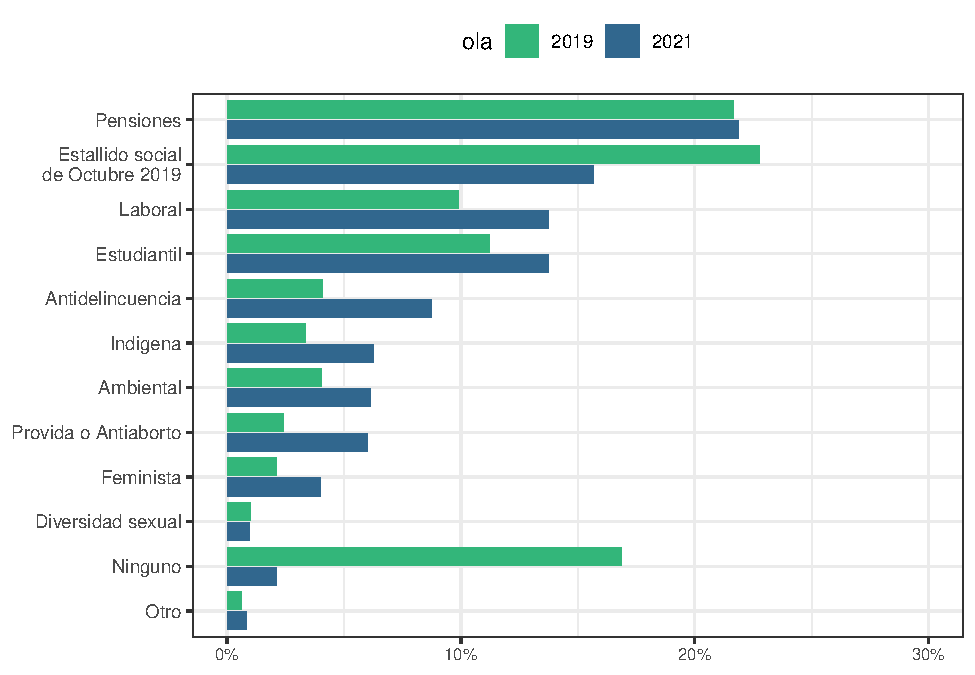
\includegraphics{reporte-elsoc_files/figure-latex/unnamed-chunk-6-1.pdf}

\hypertarget{frecuencia-de-respuesta-en-ninguno-ante-la-pregunta-cuuxe1l-es-el-movimiento-social-que-usted-muxe1s-valora-de-esta-lista-seguxfan-posiciuxf3n-poluxedtica}{%
\subsection{1.2 Frecuencia de respuesta en ``ninguno'' ante la pregunta ¿Cuál es el movimiento social que usted más valora de esta lista? según posición política"}\label{frecuencia-de-respuesta-en-ninguno-ante-la-pregunta-cuuxe1l-es-el-movimiento-social-que-usted-muxe1s-valora-de-esta-lista-seguxfan-posiciuxf3n-poluxedtica}}

\begin{Shaded}
\begin{Highlighting}[]
\NormalTok{elsoc\_long\_2016\_2021 }\SpecialCharTok{\%\textgreater{}\%}
  \FunctionTok{filter}\NormalTok{(tipo\_atricion }\SpecialCharTok{==} \DecValTok{1} \SpecialCharTok{\&}\NormalTok{ muestra }\SpecialCharTok{==} \DecValTok{1} \SpecialCharTok{\&} \SpecialCharTok{!}\NormalTok{c20 }\SpecialCharTok{\%in\%} \FunctionTok{c}\NormalTok{(}\SpecialCharTok{{-}}\DecValTok{888}\NormalTok{,}\SpecialCharTok{{-}}\DecValTok{999}\NormalTok{) }\SpecialCharTok{\&} \SpecialCharTok{!}\NormalTok{c15 }\SpecialCharTok{\%in\%} \FunctionTok{c}\NormalTok{(}\SpecialCharTok{{-}}\DecValTok{888}\NormalTok{,}\SpecialCharTok{{-}}\DecValTok{999}\NormalTok{)) }\SpecialCharTok{\%\textgreater{}\%}
  \FunctionTok{mutate}\NormalTok{(}\AttributeTok{pos\_id =} \FunctionTok{factor}\NormalTok{(car}\SpecialCharTok{::}\FunctionTok{recode}\NormalTok{(c15, }\AttributeTok{recodes =} \StringTok{"0:4 = 1; 5 = 2; 6:10 = 3; 11:12 = 4"}\NormalTok{),}
                       \AttributeTok{levels =} \FunctionTok{c}\NormalTok{(}\DecValTok{1}\NormalTok{, }\DecValTok{2}\NormalTok{, }\DecValTok{3}\NormalTok{, }\DecValTok{4}\NormalTok{),}
                       \AttributeTok{labels =} \FunctionTok{c}\NormalTok{(}\StringTok{\textquotesingle{}Izquierda\textquotesingle{}}\NormalTok{, }\StringTok{"Centro"}\NormalTok{, }\StringTok{"Derecha"}\NormalTok{, }\StringTok{"No se identifica"}\NormalTok{))) }\SpecialCharTok{\%\textgreater{}\%}
  \FunctionTok{prop}\NormalTok{(c20 }\SpecialCharTok{\%in\%} \FunctionTok{c}\NormalTok{(}\DecValTok{12}\NormalTok{), }\AttributeTok{by =} \FunctionTok{c}\NormalTok{(pos\_id, ola), }\AttributeTok{na.rm =} \ConstantTok{TRUE}\NormalTok{) }\SpecialCharTok{\%\textgreater{}\%} 
\NormalTok{  sjlabelled}\SpecialCharTok{::}\FunctionTok{as\_label}\NormalTok{(ola) }\SpecialCharTok{\%\textgreater{}\%}
  \FunctionTok{ggplot}\NormalTok{(}\FunctionTok{aes}\NormalTok{(}\AttributeTok{y =}\NormalTok{ prop, }\AttributeTok{x =}\NormalTok{ ola, }\AttributeTok{fill =}\NormalTok{ pos\_id, }
               \AttributeTok{label =}\NormalTok{ scales}\SpecialCharTok{::}\FunctionTok{percent}\NormalTok{(prop, }\AttributeTok{accuracy =}\NormalTok{ .}\DecValTok{1}\NormalTok{))) }\SpecialCharTok{+}
  \FunctionTok{theme\_bw}\NormalTok{() }\SpecialCharTok{+} 
    \FunctionTok{geom\_col}\NormalTok{(}\AttributeTok{position =} \StringTok{\textquotesingle{}dodge2\textquotesingle{}}\NormalTok{) }\SpecialCharTok{+}
    \FunctionTok{scale\_y\_continuous}\NormalTok{(}\AttributeTok{labels =}\NormalTok{ scales}\SpecialCharTok{::}\NormalTok{percent,}
                       \AttributeTok{limits =} \FunctionTok{c}\NormalTok{(}\DecValTok{0}\NormalTok{, }\DecValTok{1}\NormalTok{)) }\SpecialCharTok{+}
    \FunctionTok{ylab}\NormalTok{(}\AttributeTok{label =} \ConstantTok{NULL}\NormalTok{) }\SpecialCharTok{+}
    \FunctionTok{xlab}\NormalTok{(}\AttributeTok{label =} \ConstantTok{NULL}\NormalTok{) }\SpecialCharTok{+}
    \FunctionTok{scale\_fill\_viridis\_d}\NormalTok{(}\AttributeTok{begin =} \DecValTok{0}\NormalTok{, }\AttributeTok{end =}\NormalTok{ .}\DecValTok{85}\NormalTok{, }\AttributeTok{direction =} \SpecialCharTok{{-}}\DecValTok{1}\NormalTok{, }\AttributeTok{option =} \StringTok{\textquotesingle{}viridis\textquotesingle{}}\NormalTok{) }\SpecialCharTok{+}
    \FunctionTok{theme}\NormalTok{(}\AttributeTok{legend.position =} \StringTok{\textquotesingle{}top\textquotesingle{}}\NormalTok{,}
          \AttributeTok{legend.title =} \FunctionTok{element\_blank}\NormalTok{()) }
\end{Highlighting}
\end{Shaded}

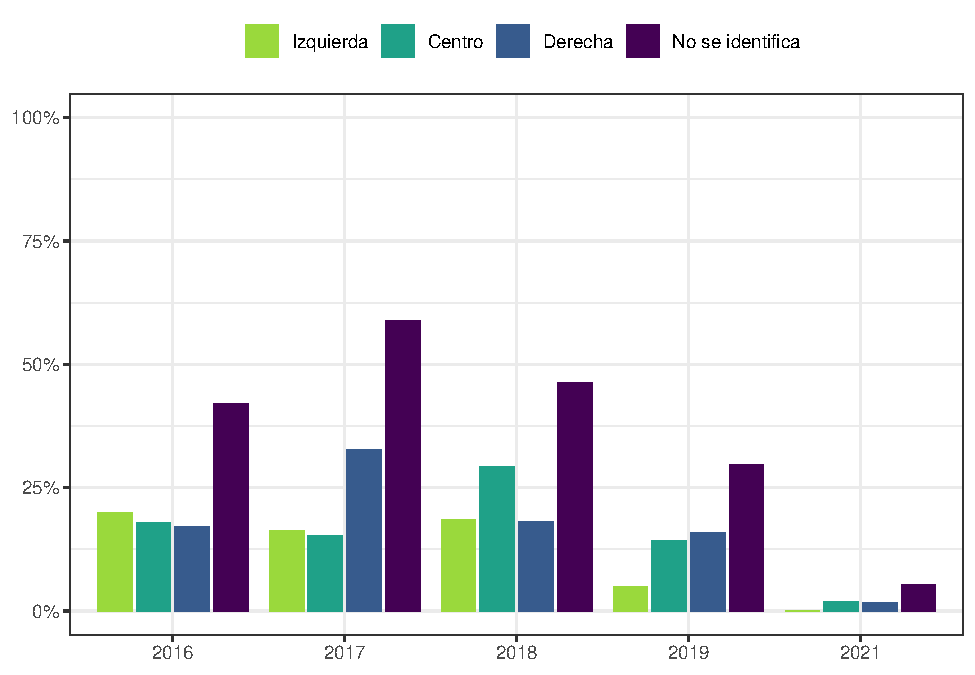
\includegraphics{reporte-elsoc_files/figure-latex/unnamed-chunk-7-1.pdf}

\hypertarget{alluvial-de-movimiento-social-que-muxe1s-valora}{%
\subsection{1.3 Alluvial de movimiento social que más valora}\label{alluvial-de-movimiento-social-que-muxe1s-valora}}

\begin{Shaded}
\begin{Highlighting}[]
\NormalTok{datos.}\FloatTok{1.3} \OtherTok{\textless{}{-}}\NormalTok{ elsoc\_long\_2016\_2021 }\SpecialCharTok{\%\textgreater{}\%}
  \FunctionTok{filter}\NormalTok{(tipo\_atricion }\SpecialCharTok{==} \DecValTok{1} \SpecialCharTok{\&} \SpecialCharTok{!}\NormalTok{c15 }\SpecialCharTok{\%in\%} \FunctionTok{c}\NormalTok{(}\SpecialCharTok{{-}}\DecValTok{888}\NormalTok{, }\SpecialCharTok{{-}}\DecValTok{999}\NormalTok{)) }\SpecialCharTok{\%\textgreater{}\%} 
  \FunctionTok{mutate}\NormalTok{(}\AttributeTok{movsoc =}\NormalTok{ car}\SpecialCharTok{::}\FunctionTok{recode}\NormalTok{(c20, }\StringTok{"1:5 = 1; 8:10 = 1; 6:7 = 2; 11:12 = 3"}\NormalTok{),}
         \AttributeTok{movsoc =} \FunctionTok{factor}\NormalTok{(movsoc, }\AttributeTok{levels =} \FunctionTok{c}\NormalTok{(}\DecValTok{1}\NormalTok{,}\DecValTok{2}\NormalTok{,}\DecValTok{3}\NormalTok{),}
                         \AttributeTok{labels =} \FunctionTok{c}\NormalTok{(}\StringTok{\textquotesingle{}Progresista\textquotesingle{}}\NormalTok{, }\StringTok{"Conservador"}\NormalTok{, }\StringTok{"Ninguno"}\NormalTok{))) }\SpecialCharTok{\%\textgreater{}\%}
  \FunctionTok{group\_by}\NormalTok{(idencuesta) }\SpecialCharTok{\%\textgreater{}\%}
  \FunctionTok{mutate}\NormalTok{(}\AttributeTok{n\_obs =} \FunctionTok{n}\NormalTok{()) }\SpecialCharTok{\%\textgreater{}\%}
  \FunctionTok{ungroup}\NormalTok{() }\SpecialCharTok{\%\textgreater{}\%} 
  \FunctionTok{mutate}\NormalTok{(}\AttributeTok{n\_ok =}\NormalTok{ (n\_obs }\SpecialCharTok{==} \FunctionTok{max}\NormalTok{(n\_obs))) }\SpecialCharTok{\%\textgreater{}\%} 
\NormalTok{  dplyr}\SpecialCharTok{::}\FunctionTok{filter}\NormalTok{(n\_ok) }\SpecialCharTok{\%\textgreater{}\%}  \CommentTok{\# Quedarse solo con los casos con observaciones completas}
  \FunctionTok{group\_by}\NormalTok{(idencuesta, movsoc, ola) }\SpecialCharTok{\%\textgreater{}\%} 
  \FunctionTok{summarise}\NormalTok{(}\AttributeTok{n1 =} \FunctionTok{sum}\NormalTok{(ponderador02, }\AttributeTok{na.rm =} \ConstantTok{TRUE}\NormalTok{)) }\SpecialCharTok{\%\textgreater{}\%}
  \FunctionTok{group\_by}\NormalTok{(ola) }\SpecialCharTok{\%\textgreater{}\%} 
  \FunctionTok{mutate}\NormalTok{(}\AttributeTok{n2 =} \FunctionTok{sum}\NormalTok{(n1, }\AttributeTok{na.rm =} \ConstantTok{TRUE}\NormalTok{), }\AttributeTok{porcentaje =}\NormalTok{ n1}\SpecialCharTok{/}\NormalTok{n2) }\SpecialCharTok{\%\textgreater{}\%} 
\NormalTok{  sjlabelled}\SpecialCharTok{::}\FunctionTok{as\_label}\NormalTok{(ola) }\SpecialCharTok{\%\textgreater{}\%} 
  \FunctionTok{ungroup}\NormalTok{()}

\NormalTok{etiquetas.}\FloatTok{1.3} \OtherTok{\textless{}{-}}\NormalTok{ datos.}\FloatTok{1.3} \SpecialCharTok{\%\textgreater{}\%} 
  \FunctionTok{group\_by}\NormalTok{(movsoc, ola) }\SpecialCharTok{\%\textgreater{}\%} 
  \FunctionTok{summarise}\NormalTok{(}\AttributeTok{porcentaje =} \FunctionTok{sum}\NormalTok{(porcentaje, }\AttributeTok{na.rm =} \ConstantTok{TRUE}\NormalTok{)) }\SpecialCharTok{\%\textgreater{}\%} 
  \FunctionTok{mutate}\NormalTok{(}\AttributeTok{idencuesta =} \DecValTok{1}\NormalTok{)}

\NormalTok{g1}\FloatTok{.3} \OtherTok{\textless{}{-}} \FunctionTok{ggplot}\NormalTok{(datos.}\FloatTok{1.3}\NormalTok{ , }\FunctionTok{aes}\NormalTok{(}\AttributeTok{x =}\NormalTok{ ola, }\AttributeTok{fill =}\NormalTok{ movsoc, }\AttributeTok{stratum =}\NormalTok{ movsoc, }
                  \AttributeTok{alluvium =}\NormalTok{ idencuesta, }\AttributeTok{y =}\NormalTok{ porcentaje )) }\SpecialCharTok{+}
  \FunctionTok{theme\_bw}\NormalTok{() }\SpecialCharTok{+}
\NormalTok{  ggalluvial}\SpecialCharTok{::}\FunctionTok{geom\_flow}\NormalTok{(}\AttributeTok{alpha =}\NormalTok{ .}\DecValTok{66}\NormalTok{) }\SpecialCharTok{+} 
\NormalTok{  ggalluvial}\SpecialCharTok{::}\FunctionTok{geom\_stratum}\NormalTok{(}\AttributeTok{linetype =} \DecValTok{0}\NormalTok{) }\SpecialCharTok{+}
  \FunctionTok{scale\_y\_continuous}\NormalTok{(}\AttributeTok{labels =}\NormalTok{ scales}\SpecialCharTok{::}\NormalTok{percent) }\SpecialCharTok{+} 
  \FunctionTok{ylab}\NormalTok{(}\AttributeTok{label =} \ConstantTok{NULL}\NormalTok{) }\SpecialCharTok{+}
  \FunctionTok{xlab}\NormalTok{(}\AttributeTok{label =} \ConstantTok{NULL}\NormalTok{) }\SpecialCharTok{+} 
  \FunctionTok{theme}\NormalTok{(}\AttributeTok{legend.position =} \StringTok{\textquotesingle{}top\textquotesingle{}}\NormalTok{,}
        \AttributeTok{legend.title =} \FunctionTok{element\_blank}\NormalTok{()) }\SpecialCharTok{+}
  \FunctionTok{scale\_fill\_viridis\_d}\NormalTok{(}\AttributeTok{begin =} \DecValTok{0}\NormalTok{, }\AttributeTok{end =}\NormalTok{ .}\DecValTok{85}\NormalTok{, }\AttributeTok{direction =} \SpecialCharTok{{-}}\DecValTok{1}\NormalTok{, }\AttributeTok{option =} \StringTok{\textquotesingle{}viridis\textquotesingle{}}\NormalTok{) }\SpecialCharTok{+}
  \FunctionTok{geom\_text}\NormalTok{(}\AttributeTok{data =}\NormalTok{ etiquetas.}\FloatTok{1.3}\NormalTok{, }
            \FunctionTok{aes}\NormalTok{(}\AttributeTok{label =}\NormalTok{ scales}\SpecialCharTok{::}\FunctionTok{percent}\NormalTok{(porcentaje, }\AttributeTok{accuracy =}\NormalTok{ .}\DecValTok{1}\NormalTok{)),}
            \AttributeTok{position =} \FunctionTok{position\_stack}\NormalTok{(}\AttributeTok{vjust =}\NormalTok{ .}\DecValTok{5}\NormalTok{),}
            \AttributeTok{show.legend =} \ConstantTok{FALSE}\NormalTok{,}
            \AttributeTok{size =} \FloatTok{2.75}\NormalTok{)}

\NormalTok{g1}\FloatTok{.3}
\end{Highlighting}
\end{Shaded}

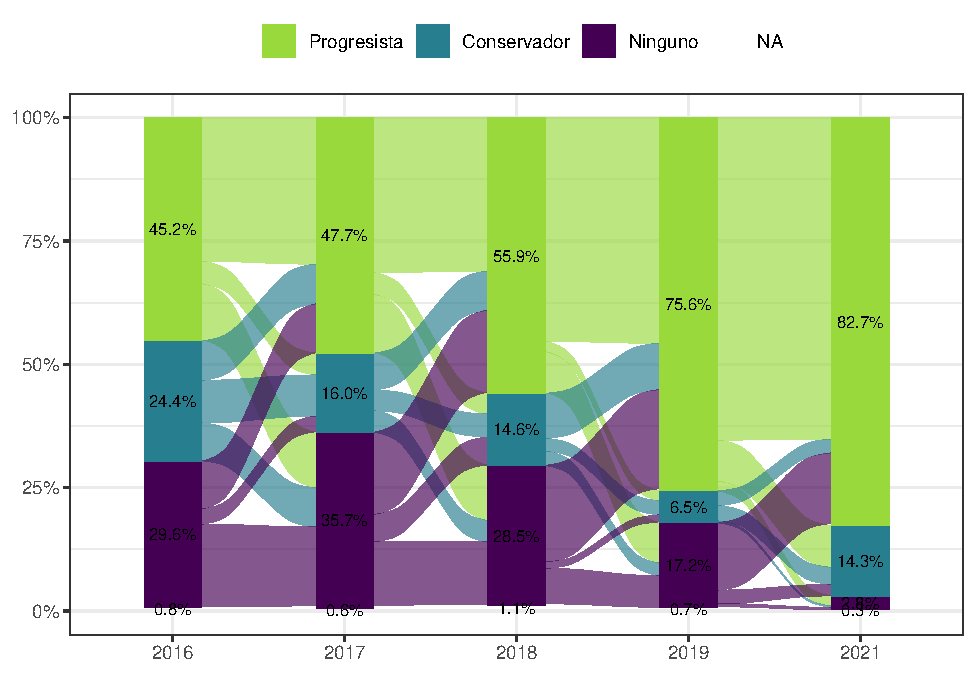
\includegraphics{reporte-elsoc_files/figure-latex/unnamed-chunk-8-1.pdf}

La determinación entre las categorías ``Progresista'' y ``Conservador'' se hizo en base a la siguiente agrupación de movimientos sociales:

Progresista: Movimiento social de apoyo a la causa estudiantil, Movimiento social de apoyo a demandas laborales, Movimiento social de grupos ambientalistas, Movimiento social de apoyo a las demandas indígena, Movimiento social de apoyo a la diversidad sexual, Movimiento feminista o de apoyo a la igualdad de género, Movimiento por el cambio al sistema de pensiones, Estallido social del 18 de Octubre de 2019

Conservador: Movimiento social provida o antiaborto, Movimiento social antidelincuencia

\hypertarget{descriptivos-generales}{%
\subsection{1.4 Descriptivos generales}\label{descriptivos-generales}}

\begin{Shaded}
\begin{Highlighting}[]
\NormalTok{elsoc\_long\_2016\_2021 }\SpecialCharTok{\%\textgreater{}\%}
    \FunctionTok{filter}\NormalTok{(tipo\_atricion }\SpecialCharTok{==} \DecValTok{1} \SpecialCharTok{\&} \SpecialCharTok{!}\NormalTok{c20 }\SpecialCharTok{\%in\%} \FunctionTok{c}\NormalTok{(}\SpecialCharTok{{-}}\DecValTok{888}\NormalTok{, }\SpecialCharTok{{-}}\DecValTok{999}\NormalTok{)) }\SpecialCharTok{\%\textgreater{}\%}
    \FunctionTok{mutate}\NormalTok{(}\AttributeTok{movsoc =}\NormalTok{ car}\SpecialCharTok{::}\FunctionTok{recode}\NormalTok{(c20, }\StringTok{"1:5 = 1; 8:10 = 1; 6:7 = 2; 11:12 = 3"}\NormalTok{),}
         \AttributeTok{movsoc =} \FunctionTok{factor}\NormalTok{(movsoc, }\AttributeTok{levels =} \FunctionTok{c}\NormalTok{(}\DecValTok{3}\NormalTok{, }\DecValTok{2}\NormalTok{, }\DecValTok{1}\NormalTok{),}
                         \AttributeTok{labels =} \FunctionTok{c}\NormalTok{(}\StringTok{\textquotesingle{}Ninguno\textquotesingle{}}\NormalTok{, }\StringTok{\textquotesingle{}Conservador\textquotesingle{}}\NormalTok{, }\StringTok{\textquotesingle{}Progresista\textquotesingle{}}\NormalTok{))) }\SpecialCharTok{\%\textgreater{}\%}
\NormalTok{    dplyr}\SpecialCharTok{::}\FunctionTok{filter}\NormalTok{(}\SpecialCharTok{!}\FunctionTok{is.na}\NormalTok{(movsoc)) }\SpecialCharTok{\%\textgreater{}\%}
    \FunctionTok{prop}\NormalTok{(movsoc, }\AttributeTok{by  =} \FunctionTok{c}\NormalTok{(ola), }\AttributeTok{na.rm =} \ConstantTok{TRUE}\NormalTok{)  }\SpecialCharTok{\%\textgreater{}\%} 
\NormalTok{    sjlabelled}\SpecialCharTok{::}\FunctionTok{as\_label}\NormalTok{(ola) }\SpecialCharTok{\%\textgreater{}\%} 
    \FunctionTok{ggplot}\NormalTok{(}\FunctionTok{aes}\NormalTok{(}\AttributeTok{y =}\NormalTok{ prop, }\AttributeTok{x =}\NormalTok{ movsoc, }\AttributeTok{fill =}\NormalTok{ ola, }
               \AttributeTok{label =}\NormalTok{ scales}\SpecialCharTok{::}\FunctionTok{percent}\NormalTok{(prop, }\AttributeTok{accuracy =}\NormalTok{ .}\DecValTok{1}\NormalTok{))) }\SpecialCharTok{+}
    \FunctionTok{theme\_bw}\NormalTok{() }\SpecialCharTok{+} 
    \FunctionTok{geom\_col}\NormalTok{(}\AttributeTok{position=} \StringTok{\textquotesingle{}dodge2\textquotesingle{}}\NormalTok{) }\SpecialCharTok{+}
    \FunctionTok{scale\_y\_continuous}\NormalTok{(}\AttributeTok{labels =}\NormalTok{ scales}\SpecialCharTok{::}\NormalTok{percent,}
                       \AttributeTok{limits =} \FunctionTok{c}\NormalTok{(}\DecValTok{0}\NormalTok{, }\DecValTok{1}\NormalTok{)) }\SpecialCharTok{+}
    \FunctionTok{ylab}\NormalTok{(}\AttributeTok{label =} \ConstantTok{NULL}\NormalTok{) }\SpecialCharTok{+}
    \FunctionTok{xlab}\NormalTok{(}\AttributeTok{label =} \ConstantTok{NULL}\NormalTok{) }\SpecialCharTok{+}
    \FunctionTok{scale\_fill\_viridis\_d}\NormalTok{(}\AttributeTok{begin =} \DecValTok{0}\NormalTok{, }\AttributeTok{end =}\NormalTok{ .}\DecValTok{85}\NormalTok{, }\AttributeTok{direction =} \SpecialCharTok{{-}}\DecValTok{1}\NormalTok{, }\AttributeTok{option =} \StringTok{\textquotesingle{}viridis\textquotesingle{}}\NormalTok{) }\SpecialCharTok{+}
    \FunctionTok{geom\_text}\NormalTok{(}\AttributeTok{hjust =} \SpecialCharTok{{-}}\NormalTok{.}\DecValTok{1}\NormalTok{,}
            \AttributeTok{position =} \FunctionTok{position\_dodge}\NormalTok{(}\AttributeTok{width =} \DecValTok{1}\NormalTok{),}
            \AttributeTok{size=} \FloatTok{2.75}\NormalTok{) }\SpecialCharTok{+}
    \FunctionTok{theme}\NormalTok{(}\AttributeTok{legend.position =} \StringTok{\textquotesingle{}top\textquotesingle{}}\NormalTok{,}
          \AttributeTok{legend.title =} \FunctionTok{element\_blank}\NormalTok{()) }\SpecialCharTok{+}
  \FunctionTok{coord\_flip}\NormalTok{()}
\end{Highlighting}
\end{Shaded}

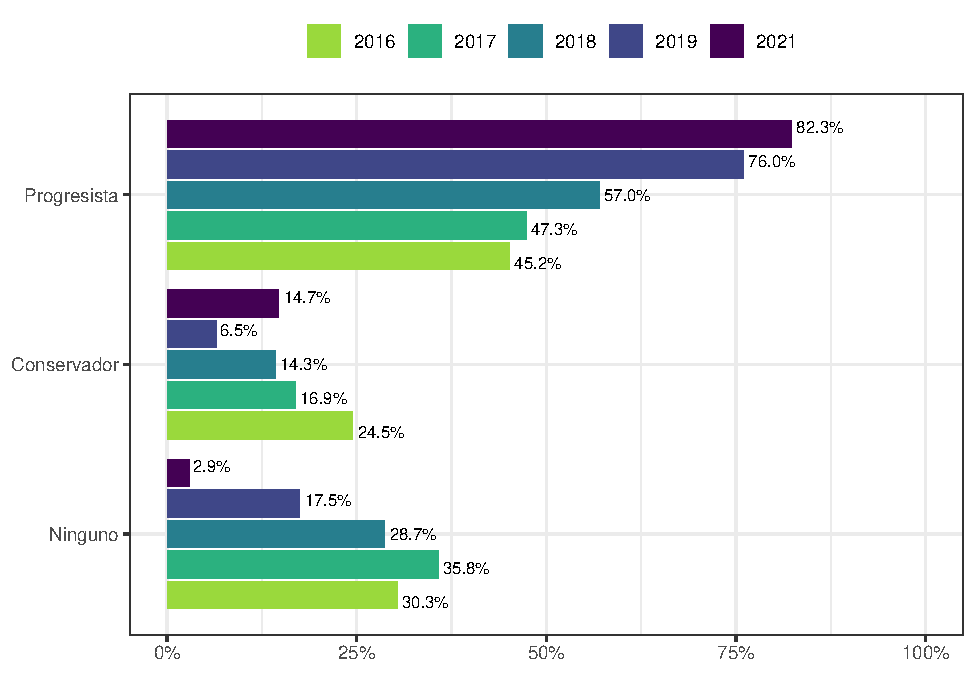
\includegraphics{reporte-elsoc_files/figure-latex/unnamed-chunk-9-1.pdf}

\hypertarget{cambios-en-la-valoraciuxf3n-de-movimientos-sociales-seguxfan-posiciuxf3n-poluxedtica}{%
\subsection{1.5 Cambios en la valoración de movimientos sociales según posición política}\label{cambios-en-la-valoraciuxf3n-de-movimientos-sociales-seguxfan-posiciuxf3n-poluxedtica}}

\begin{Shaded}
\begin{Highlighting}[]
\NormalTok{datos.}\FloatTok{1.5} \OtherTok{\textless{}{-}}\NormalTok{elsoc\_long\_2016\_2021 }\SpecialCharTok{\%\textgreater{}\%}
  \FunctionTok{filter}\NormalTok{(tipo\_atricion }\SpecialCharTok{==} \DecValTok{1} \SpecialCharTok{\&}\NormalTok{ ola }\SpecialCharTok{\%in\%} \FunctionTok{c}\NormalTok{(}\DecValTok{3}\NormalTok{,}\DecValTok{4}\NormalTok{,}\DecValTok{5}\NormalTok{)) }\SpecialCharTok{\%\textgreater{}\%}
 \FunctionTok{mutate}\NormalTok{(}\AttributeTok{movsoc =}\NormalTok{ car}\SpecialCharTok{::}\FunctionTok{recode}\NormalTok{(c20, }\AttributeTok{recodes =} \StringTok{"1=\textquotesingle{}1\textquotesingle{};2=\textquotesingle{}1\textquotesingle{};3=\textquotesingle{}1\textquotesingle{};}
\StringTok{                                          4=\textquotesingle{}1\textquotesingle{};5=\textquotesingle{}1\textquotesingle{};6=\textquotesingle{}2\textquotesingle{};7=\textquotesingle{}2\textquotesingle{};}
\StringTok{                                          8=\textquotesingle{}1\textquotesingle{};9=\textquotesingle{}1\textquotesingle{};10=\textquotesingle{}1\textquotesingle{};11=NA;12=\textquotesingle{}3\textquotesingle{};}
\StringTok{                                          c({-}999,{-}888)=NA"}\NormalTok{,}\AttributeTok{as.factor=}\NormalTok{T)) }\SpecialCharTok{\%\textgreater{}\%} 
   \FunctionTok{mutate}\NormalTok{(}\AttributeTok{movsoc =} \FunctionTok{factor}\NormalTok{(movsoc, }\AttributeTok{levels =} \FunctionTok{c}\NormalTok{(}\DecValTok{1}\NormalTok{,}\DecValTok{2}\NormalTok{,}\DecValTok{3}\NormalTok{),}
                         \AttributeTok{labels =} \FunctionTok{c}\NormalTok{(}\StringTok{\textquotesingle{}Progresista\textquotesingle{}}\NormalTok{, }\StringTok{"Conservador"}\NormalTok{, }\StringTok{"Ninguno"}\NormalTok{)),}
          \AttributeTok{pos\_id =} \FunctionTok{factor}\NormalTok{(car}\SpecialCharTok{::}\FunctionTok{recode}\NormalTok{(c15, }\AttributeTok{recodes =} \StringTok{"0:4 = 1; 5 = 2; 6:10 = 3; 11:12 = 4"}\NormalTok{),}
                       \AttributeTok{levels =} \FunctionTok{c}\NormalTok{(}\DecValTok{1}\NormalTok{, }\DecValTok{2}\NormalTok{, }\DecValTok{3}\NormalTok{, }\DecValTok{4}\NormalTok{),}
                       \AttributeTok{labels =} \FunctionTok{c}\NormalTok{(}\StringTok{\textquotesingle{}Izquierda\textquotesingle{}}\NormalTok{, }\StringTok{"Centro"}\NormalTok{, }\StringTok{"Derecha"}\NormalTok{, }\StringTok{"No se identifica"}\NormalTok{))) }\SpecialCharTok{\%\textgreater{}\%}
\NormalTok{  dplyr}\SpecialCharTok{::}\FunctionTok{filter}\NormalTok{(}\SpecialCharTok{!}\FunctionTok{is.na}\NormalTok{(pos\_id) }\SpecialCharTok{\&} \SpecialCharTok{!}\FunctionTok{is.na}\NormalTok{(movsoc)) }\SpecialCharTok{\%\textgreater{}\%}
  \FunctionTok{prop}\NormalTok{(movsoc, }\AttributeTok{by  =} \FunctionTok{c}\NormalTok{(ola, pos\_id), }\AttributeTok{na.rm =} \ConstantTok{TRUE}\NormalTok{)}\SpecialCharTok{\%\textgreater{}\%} 
\NormalTok{  sjlabelled}\SpecialCharTok{::}\FunctionTok{as\_label}\NormalTok{(ola)}

\NormalTok{g1}\FloatTok{.5} \OtherTok{\textless{}{-}}\NormalTok{ datos.}\FloatTok{1.5} \SpecialCharTok{\%\textgreater{}\%} 
  \FunctionTok{ggplot}\NormalTok{(}\FunctionTok{aes}\NormalTok{(}\AttributeTok{y =}\NormalTok{ prop, }\AttributeTok{x =}\NormalTok{ pos\_id, }\AttributeTok{fill =}\NormalTok{movsoc, }
             \AttributeTok{label =} \FunctionTok{as.character}\NormalTok{(scales}\SpecialCharTok{::}\FunctionTok{percent}\NormalTok{(}\FunctionTok{ifelse}\NormalTok{(prop}\SpecialCharTok{\textgreater{}}\NormalTok{.}\DecValTok{01}\NormalTok{, prop, }\ConstantTok{NA}\NormalTok{), }\AttributeTok{accuracy =}\NormalTok{ .}\DecValTok{1}\NormalTok{)))) }\SpecialCharTok{+}
  \FunctionTok{theme\_bw}\NormalTok{() }\SpecialCharTok{+}
  \FunctionTok{geom\_col}\NormalTok{(}\AttributeTok{position =} \StringTok{\textquotesingle{}stack\textquotesingle{}}\NormalTok{) }\SpecialCharTok{+}
  \FunctionTok{facet\_grid}\NormalTok{(.}\SpecialCharTok{\textasciitilde{}}\NormalTok{ola) }\SpecialCharTok{+}
  \FunctionTok{scale\_y\_continuous}\NormalTok{(}\AttributeTok{labels =}\NormalTok{ scales}\SpecialCharTok{::}\NormalTok{percent) }\SpecialCharTok{+}
  \FunctionTok{ylab}\NormalTok{(}\AttributeTok{label =} \ConstantTok{NULL}\NormalTok{) }\SpecialCharTok{+}
  \FunctionTok{xlab}\NormalTok{(}\AttributeTok{label =} \ConstantTok{NULL}\NormalTok{) }\SpecialCharTok{+}
  \FunctionTok{scale\_fill\_viridis\_d}\NormalTok{(}\AttributeTok{begin =} \DecValTok{0}\NormalTok{, }\AttributeTok{end =}\NormalTok{ .}\DecValTok{85}\NormalTok{, }\AttributeTok{direction =} \SpecialCharTok{{-}}\DecValTok{1}\NormalTok{, }\AttributeTok{option =} \StringTok{\textquotesingle{}viridis\textquotesingle{}}\NormalTok{) }\SpecialCharTok{+}
  \FunctionTok{geom\_text}\NormalTok{(}\AttributeTok{position =} \FunctionTok{position\_stack}\NormalTok{(}\AttributeTok{vjust =}\NormalTok{ .}\DecValTok{5}\NormalTok{),}
            \AttributeTok{size=} \FloatTok{2.75}\NormalTok{,}
            \AttributeTok{color =} \FunctionTok{rep}\NormalTok{(}\FunctionTok{c}\NormalTok{(}\FunctionTok{rep}\NormalTok{(}\StringTok{\textquotesingle{}white\textquotesingle{}}\NormalTok{, }\DecValTok{4}\NormalTok{),}
                          \FunctionTok{rep}\NormalTok{(}\StringTok{\textquotesingle{}white\textquotesingle{}}\NormalTok{, }\DecValTok{4}\NormalTok{),}
                          \FunctionTok{rep}\NormalTok{(}\StringTok{\textquotesingle{}white\textquotesingle{}}\NormalTok{, }\DecValTok{4}\NormalTok{)),}\DecValTok{3}\NormalTok{)) }\SpecialCharTok{+} 
  \FunctionTok{theme}\NormalTok{(}\AttributeTok{legend.position =} \StringTok{\textquotesingle{}top\textquotesingle{}}\NormalTok{,}
        \AttributeTok{legend.title =} \FunctionTok{element\_blank}\NormalTok{()) }
\NormalTok{g1}\FloatTok{.5}
\end{Highlighting}
\end{Shaded}

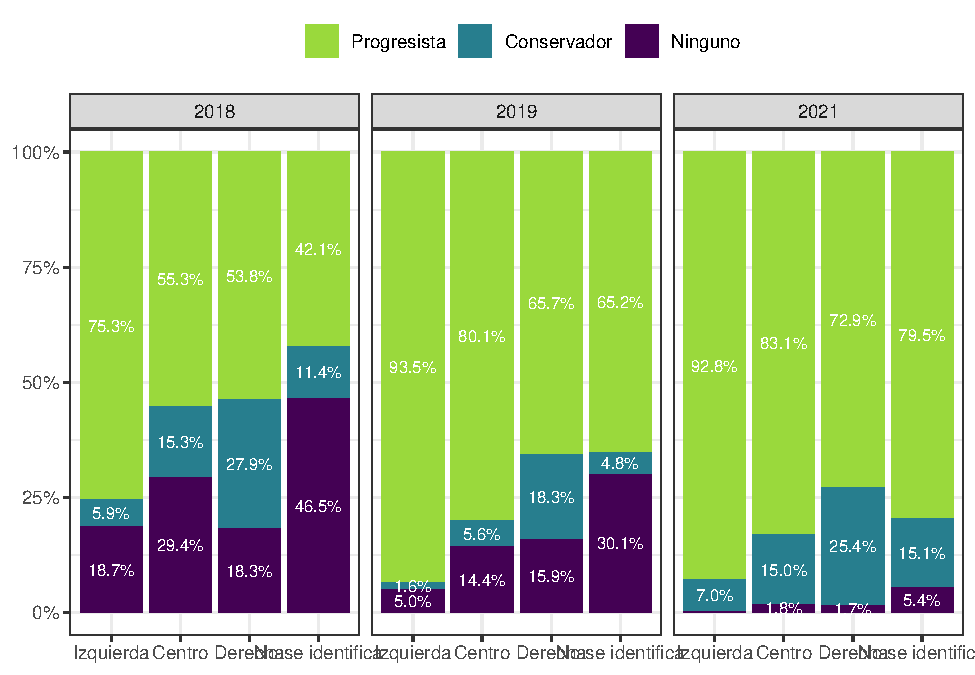
\includegraphics{reporte-elsoc_files/figure-latex/unnamed-chunk-10-1.pdf}

\hypertarget{cambios-en-la-valoraciuxf3n-de-movimientos-sociales-seguxfan-nivel-educativo}{%
\subsection{1.6 Cambios en la valoración de movimientos sociales según nivel educativo}\label{cambios-en-la-valoraciuxf3n-de-movimientos-sociales-seguxfan-nivel-educativo}}

\begin{Shaded}
\begin{Highlighting}[]
\NormalTok{datos.}\FloatTok{1.6} \OtherTok{\textless{}{-}}\NormalTok{ elsoc\_long\_2016\_2021 }\SpecialCharTok{\%\textgreater{}\%}
  \FunctionTok{filter}\NormalTok{(tipo\_atricion }\SpecialCharTok{==} \DecValTok{1} \SpecialCharTok{\&} \SpecialCharTok{!}\NormalTok{ola }\SpecialCharTok{\%in\%} \FunctionTok{c}\NormalTok{(}\DecValTok{1}\NormalTok{)) }\SpecialCharTok{\%\textgreater{}\%}
   \FunctionTok{mutate}\NormalTok{(}\AttributeTok{movsoc =}\NormalTok{ car}\SpecialCharTok{::}\FunctionTok{recode}\NormalTok{(c20, }\AttributeTok{recodes =} \StringTok{"1=\textquotesingle{}1\textquotesingle{};2=\textquotesingle{}1\textquotesingle{};3=\textquotesingle{}1\textquotesingle{};}
\StringTok{                                          4=\textquotesingle{}1\textquotesingle{};5=\textquotesingle{}1\textquotesingle{};6=\textquotesingle{}2\textquotesingle{};7=\textquotesingle{}2\textquotesingle{};}
\StringTok{                                          8=\textquotesingle{}1\textquotesingle{};9=\textquotesingle{}1\textquotesingle{};10=\textquotesingle{}1\textquotesingle{};11=NA;12=\textquotesingle{}3\textquotesingle{};}
\StringTok{                                          c({-}999,{-}888)=NA"}\NormalTok{,}\AttributeTok{as.factor=}\NormalTok{T)) }\SpecialCharTok{\%\textgreater{}\%} 
   \FunctionTok{mutate}\NormalTok{(}\AttributeTok{movsoc =} \FunctionTok{factor}\NormalTok{(movsoc, }\AttributeTok{levels =} \FunctionTok{c}\NormalTok{(}\DecValTok{1}\NormalTok{,}\DecValTok{2}\NormalTok{,}\DecValTok{3}\NormalTok{),}
                         \AttributeTok{labels =} \FunctionTok{c}\NormalTok{(}\StringTok{\textquotesingle{}Progresista\textquotesingle{}}\NormalTok{, }\StringTok{"Conservador"}\NormalTok{, }\StringTok{"Ninguno"}\NormalTok{))) }\SpecialCharTok{\%\textgreater{}\%}
  \FunctionTok{mutate}\NormalTok{(}\AttributeTok{educ =}\NormalTok{ car}\SpecialCharTok{::}\FunctionTok{recode}\NormalTok{(m01, }\AttributeTok{recodes =} \StringTok{"c(1,2,3)=1;c(4,5)=2;c(6,7)=3;c(8,9,10)=4"}\NormalTok{)) }\SpecialCharTok{\%\textgreater{}\%}
  \FunctionTok{mutate}\NormalTok{(}\AttributeTok{educ =} \FunctionTok{factor}\NormalTok{(educ, }\AttributeTok{levels =} \FunctionTok{c}\NormalTok{(}\DecValTok{1}\NormalTok{,}\DecValTok{2}\NormalTok{,}\DecValTok{3}\NormalTok{,}\DecValTok{4}\NormalTok{),}
                         \AttributeTok{labels =} \FunctionTok{c}\NormalTok{(}\StringTok{"Basica"}\NormalTok{,}\StringTok{"Media"}\NormalTok{,}\StringTok{"Tecnica"}\NormalTok{,}\StringTok{"Universitaria"}\NormalTok{))) }\SpecialCharTok{\%\textgreater{}\%}
\NormalTok{    dplyr}\SpecialCharTok{::}\FunctionTok{filter}\NormalTok{(}\SpecialCharTok{!}\FunctionTok{is.na}\NormalTok{(educ) }\SpecialCharTok{\&} \SpecialCharTok{!}\FunctionTok{is.na}\NormalTok{(movsoc)) }\SpecialCharTok{\%\textgreater{}\%}
  \FunctionTok{prop}\NormalTok{(movsoc, }\AttributeTok{by  =} \FunctionTok{c}\NormalTok{(ola, educ), }\AttributeTok{na.rm =} \ConstantTok{TRUE}\NormalTok{)}\SpecialCharTok{\%\textgreater{}\%} 
\NormalTok{  sjlabelled}\SpecialCharTok{::}\FunctionTok{as\_label}\NormalTok{(ola)}
  
  
\NormalTok{g1}\FloatTok{.6} \OtherTok{\textless{}{-}}\NormalTok{ datos.}\FloatTok{1.6} \SpecialCharTok{\%\textgreater{}\%} 
  \FunctionTok{ggplot}\NormalTok{(}\FunctionTok{aes}\NormalTok{(}\AttributeTok{y =}\NormalTok{ prop, }\AttributeTok{x =}\NormalTok{ educ, }\AttributeTok{fill =}\NormalTok{movsoc, }
             \AttributeTok{label =} \FunctionTok{as.character}\NormalTok{(scales}\SpecialCharTok{::}\FunctionTok{percent}\NormalTok{(}\FunctionTok{ifelse}\NormalTok{(prop}\SpecialCharTok{\textgreater{}}\NormalTok{.}\DecValTok{01}\NormalTok{, prop, }\ConstantTok{NA}\NormalTok{), }\AttributeTok{accuracy =}\NormalTok{ .}\DecValTok{1}\NormalTok{)))) }\SpecialCharTok{+}
  \FunctionTok{theme\_bw}\NormalTok{() }\SpecialCharTok{+}
  \FunctionTok{geom\_col}\NormalTok{(}\AttributeTok{position =} \StringTok{\textquotesingle{}stack\textquotesingle{}}\NormalTok{) }\SpecialCharTok{+}
  \FunctionTok{facet\_grid}\NormalTok{(.}\SpecialCharTok{\textasciitilde{}}\NormalTok{ola) }\SpecialCharTok{+}
  \FunctionTok{scale\_y\_continuous}\NormalTok{(}\AttributeTok{labels =}\NormalTok{ scales}\SpecialCharTok{::}\NormalTok{percent) }\SpecialCharTok{+}
  \FunctionTok{ylab}\NormalTok{(}\AttributeTok{label =} \ConstantTok{NULL}\NormalTok{) }\SpecialCharTok{+}
  \FunctionTok{xlab}\NormalTok{(}\AttributeTok{label =} \ConstantTok{NULL}\NormalTok{) }\SpecialCharTok{+}
  \FunctionTok{scale\_fill\_viridis\_d}\NormalTok{(}\AttributeTok{begin =} \DecValTok{0}\NormalTok{, }\AttributeTok{end =}\NormalTok{ .}\DecValTok{85}\NormalTok{, }\AttributeTok{direction =} \SpecialCharTok{{-}}\DecValTok{1}\NormalTok{, }\AttributeTok{option =} \StringTok{\textquotesingle{}viridis\textquotesingle{}}\NormalTok{) }\SpecialCharTok{+}
  \FunctionTok{geom\_text}\NormalTok{(}\AttributeTok{position =} \FunctionTok{position\_stack}\NormalTok{(}\AttributeTok{vjust =}\NormalTok{ .}\DecValTok{5}\NormalTok{),}
            \AttributeTok{size=} \FloatTok{2.75}\NormalTok{,}
            \AttributeTok{color =} \FunctionTok{rep}\NormalTok{(}\FunctionTok{c}\NormalTok{(}\FunctionTok{rep}\NormalTok{(}\StringTok{\textquotesingle{}white\textquotesingle{}}\NormalTok{, }\DecValTok{4}\NormalTok{),}
                          \FunctionTok{rep}\NormalTok{(}\StringTok{\textquotesingle{}white\textquotesingle{}}\NormalTok{, }\DecValTok{4}\NormalTok{),}
                          \FunctionTok{rep}\NormalTok{(}\StringTok{\textquotesingle{}white\textquotesingle{}}\NormalTok{, }\DecValTok{4}\NormalTok{)),}\DecValTok{4}\NormalTok{)) }\SpecialCharTok{+} 
  \FunctionTok{theme}\NormalTok{(}\AttributeTok{legend.position =} \StringTok{\textquotesingle{}top\textquotesingle{}}\NormalTok{,}
        \AttributeTok{legend.title =} \FunctionTok{element\_blank}\NormalTok{())}

\NormalTok{g1}\FloatTok{.6}
\end{Highlighting}
\end{Shaded}

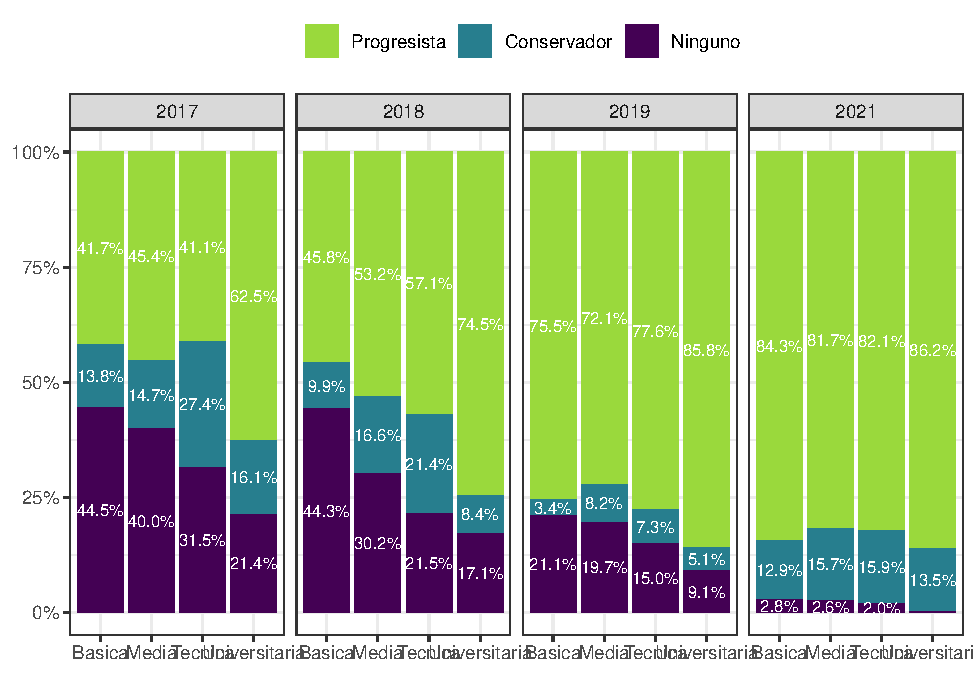
\includegraphics{reporte-elsoc_files/figure-latex/unnamed-chunk-11-1.pdf}

\hypertarget{valoraciuxf3n-de-movimientos-sociales-segun-segun-participacion}{%
\subsection{1.7 Valoración de movimientos sociales segun segun participacion}\label{valoraciuxf3n-de-movimientos-sociales-segun-segun-participacion}}

\begin{Shaded}
\begin{Highlighting}[]
\NormalTok{datos.}\FloatTok{1.7} \OtherTok{\textless{}{-}}\NormalTok{ elsoc\_long\_2016\_2021 }\SpecialCharTok{\%\textgreater{}\%}
  \FunctionTok{mutate}\NormalTok{(}\AttributeTok{movsoc =}\NormalTok{ car}\SpecialCharTok{::}\FunctionTok{recode}\NormalTok{(c20, }\AttributeTok{recodes =} \StringTok{"1=\textquotesingle{}1\textquotesingle{};2=\textquotesingle{}1\textquotesingle{};3=\textquotesingle{}1\textquotesingle{};}
\StringTok{                                          4=\textquotesingle{}1\textquotesingle{};5=\textquotesingle{}1\textquotesingle{};6=\textquotesingle{}2\textquotesingle{};7=\textquotesingle{}2\textquotesingle{};}
\StringTok{                                          8=\textquotesingle{}1\textquotesingle{};9=\textquotesingle{}1\textquotesingle{};10=\textquotesingle{}1\textquotesingle{};11=NA;12=\textquotesingle{}3\textquotesingle{};}
\StringTok{                                          c({-}999,{-}888)=NA"}\NormalTok{,}\AttributeTok{as.factor=}\NormalTok{T)) }\SpecialCharTok{\%\textgreater{}\%} 
   \FunctionTok{mutate}\NormalTok{(}\AttributeTok{movsoc =} \FunctionTok{factor}\NormalTok{(movsoc, }\AttributeTok{levels =} \FunctionTok{c}\NormalTok{(}\DecValTok{1}\NormalTok{,}\DecValTok{2}\NormalTok{,}\DecValTok{3}\NormalTok{),}
                         \AttributeTok{labels =} \FunctionTok{c}\NormalTok{(}\StringTok{\textquotesingle{}Progresista\textquotesingle{}}\NormalTok{, }\StringTok{"Conservador"}\NormalTok{, }\StringTok{"Ninguno"}\NormalTok{))) }\SpecialCharTok{\%\textgreater{}\%}
  \FunctionTok{mutate}\NormalTok{(}\AttributeTok{participacion =}\NormalTok{ car}\SpecialCharTok{::}\FunctionTok{recode}\NormalTok{(c22, }\AttributeTok{recodes =} 
                         \StringTok{"c(1,2)=\textquotesingle{}1\textquotesingle{}; 3=\textquotesingle{}2\textquotesingle{};}
\StringTok{                          c(4,5)=\textquotesingle{}3\textquotesingle{};}
\StringTok{                          c({-}999,{-}888)=NA"}\NormalTok{,}\AttributeTok{as.factor=}\NormalTok{T)) }\SpecialCharTok{\%\textgreater{}\%}
    \FunctionTok{mutate}\NormalTok{(}\AttributeTok{participacion =} \FunctionTok{factor}\NormalTok{(participacion, }\AttributeTok{levels =} \FunctionTok{c}\NormalTok{(}\DecValTok{1}\NormalTok{,}\DecValTok{2}\NormalTok{,}\DecValTok{3}\NormalTok{),}
                         \AttributeTok{labels =} \FunctionTok{c}\NormalTok{(}\StringTok{\textquotesingle{}Nunca o}\SpecialCharTok{\textbackslash{}n}\StringTok{casi nunca\textquotesingle{}}\NormalTok{, }\StringTok{\textquotesingle{}A veces\textquotesingle{}}\NormalTok{, }\StringTok{\textquotesingle{}Frecuente o}\SpecialCharTok{\textbackslash{}n}\StringTok{muy}\SpecialCharTok{\textbackslash{}n}\StringTok{frecuentemente\textquotesingle{}}\NormalTok{))) }\SpecialCharTok{\%\textgreater{}\%}
    \FunctionTok{filter}\NormalTok{(tipo\_atricion }\SpecialCharTok{==} \DecValTok{1}\NormalTok{) }\SpecialCharTok{\%\textgreater{}\%}
\NormalTok{    dplyr}\SpecialCharTok{::}\FunctionTok{filter}\NormalTok{(}\SpecialCharTok{!}\FunctionTok{is.na}\NormalTok{(participacion) }\SpecialCharTok{\&} \SpecialCharTok{!}\FunctionTok{is.na}\NormalTok{(movsoc)) }\SpecialCharTok{\%\textgreater{}\%}
  \FunctionTok{prop}\NormalTok{(movsoc, }\AttributeTok{by  =} \FunctionTok{c}\NormalTok{(ola, participacion), }\AttributeTok{na.rm =} \ConstantTok{TRUE}\NormalTok{)}\SpecialCharTok{\%\textgreater{}\%} 
\NormalTok{  sjlabelled}\SpecialCharTok{::}\FunctionTok{as\_label}\NormalTok{(ola)}

\NormalTok{g1}\FloatTok{.7} \OtherTok{\textless{}{-}}\NormalTok{ datos.}\FloatTok{1.7} \SpecialCharTok{\%\textgreater{}\%} 
  \FunctionTok{ggplot}\NormalTok{(}\FunctionTok{aes}\NormalTok{(}\AttributeTok{y =}\NormalTok{ prop, }\AttributeTok{x =}\NormalTok{ participacion, }\AttributeTok{fill =}\NormalTok{movsoc, }
             \AttributeTok{label =} \FunctionTok{as.character}\NormalTok{(scales}\SpecialCharTok{::}\FunctionTok{percent}\NormalTok{(}\FunctionTok{ifelse}\NormalTok{(prop}\SpecialCharTok{\textgreater{}}\NormalTok{.}\DecValTok{01}\NormalTok{, prop, }\ConstantTok{NA}\NormalTok{), }\AttributeTok{accuracy =}\NormalTok{ .}\DecValTok{1}\NormalTok{)))) }\SpecialCharTok{+}
  \FunctionTok{theme\_bw}\NormalTok{() }\SpecialCharTok{+}
  \FunctionTok{geom\_col}\NormalTok{(}\AttributeTok{position =} \StringTok{\textquotesingle{}stack\textquotesingle{}}\NormalTok{) }\SpecialCharTok{+}
  \FunctionTok{facet\_grid}\NormalTok{(.}\SpecialCharTok{\textasciitilde{}}\NormalTok{ola) }\SpecialCharTok{+}
  \FunctionTok{scale\_y\_continuous}\NormalTok{(}\AttributeTok{labels =}\NormalTok{ scales}\SpecialCharTok{::}\NormalTok{percent) }\SpecialCharTok{+}
  \FunctionTok{ylab}\NormalTok{(}\AttributeTok{label =} \ConstantTok{NULL}\NormalTok{) }\SpecialCharTok{+}
  \FunctionTok{xlab}\NormalTok{(}\AttributeTok{label =} \ConstantTok{NULL}\NormalTok{) }\SpecialCharTok{+}
  \FunctionTok{scale\_fill\_viridis\_d}\NormalTok{(}\AttributeTok{begin =} \DecValTok{0}\NormalTok{, }\AttributeTok{end =}\NormalTok{ .}\DecValTok{85}\NormalTok{, }\AttributeTok{direction =} \SpecialCharTok{{-}}\DecValTok{1}\NormalTok{, }\AttributeTok{option =} \StringTok{\textquotesingle{}viridis\textquotesingle{}}\NormalTok{) }\SpecialCharTok{+}
  \FunctionTok{geom\_text}\NormalTok{(}\AttributeTok{position =} \FunctionTok{position\_stack}\NormalTok{(}\AttributeTok{vjust =}\NormalTok{ .}\DecValTok{5}\NormalTok{),}
            \AttributeTok{size=} \FloatTok{2.75}\NormalTok{,}
            \AttributeTok{color =} \FunctionTok{rep}\NormalTok{(}\FunctionTok{c}\NormalTok{(}\FunctionTok{rep}\NormalTok{(}\StringTok{\textquotesingle{}white\textquotesingle{}}\NormalTok{, }\DecValTok{3}\NormalTok{),}
                          \FunctionTok{rep}\NormalTok{(}\StringTok{\textquotesingle{}white\textquotesingle{}}\NormalTok{, }\DecValTok{3}\NormalTok{)),}\DecValTok{5}\NormalTok{)) }\SpecialCharTok{+} 
  \FunctionTok{theme}\NormalTok{(}\AttributeTok{legend.position =} \StringTok{\textquotesingle{}top\textquotesingle{}}\NormalTok{,}
        \AttributeTok{legend.title =} \FunctionTok{element\_blank}\NormalTok{())}

\NormalTok{g1}\FloatTok{.7}
\end{Highlighting}
\end{Shaded}

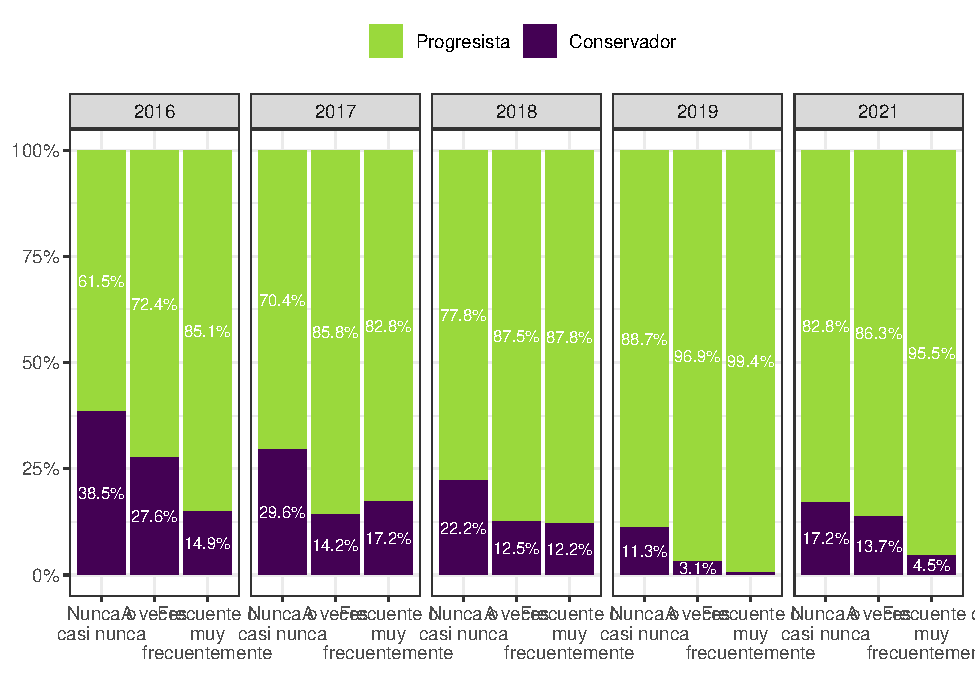
\includegraphics{reporte-elsoc_files/figure-latex/unnamed-chunk-12-1.pdf}

\hypertarget{frecuencia-de-participaciuxf3n-en-movimientos-sociales-seguxfan-ola-de-encuesta.-porcentaje-que-responde-frecuentemente-o-muy-frecuentemente}{%
\subsection{1.8 Frecuencia de participación en movimientos sociales, según Ola de encuesta. Porcentaje que responde Frecuentemente o Muy frecuentemente}\label{frecuencia-de-participaciuxf3n-en-movimientos-sociales-seguxfan-ola-de-encuesta.-porcentaje-que-responde-frecuentemente-o-muy-frecuentemente}}

\begin{Shaded}
\begin{Highlighting}[]
\NormalTok{elsoc\_long\_2016\_2021 }\SpecialCharTok{\%\textgreater{}\%}
  \FunctionTok{filter}\NormalTok{(tipo\_atricion }\SpecialCharTok{==} \DecValTok{1} \SpecialCharTok{\&}\NormalTok{ muestra}\SpecialCharTok{==}\DecValTok{1} \SpecialCharTok{\&} \SpecialCharTok{!}\NormalTok{c22 }\SpecialCharTok{\%in\%} \FunctionTok{c}\NormalTok{(}\SpecialCharTok{{-}}\DecValTok{888}\NormalTok{, }\SpecialCharTok{{-}}\DecValTok{999}\NormalTok{)) }\SpecialCharTok{\%\textgreater{}\%}
  \FunctionTok{prop}\NormalTok{(c22 }\SpecialCharTok{\%in\%} \DecValTok{4}\SpecialCharTok{:}\DecValTok{5}\NormalTok{, }\AttributeTok{by  =}\NormalTok{ ola, }\AttributeTok{na.rm =} \ConstantTok{TRUE}\NormalTok{) }\SpecialCharTok{\%\textgreater{}\%}
\NormalTok{  sjlabelled}\SpecialCharTok{::}\FunctionTok{as\_label}\NormalTok{(ola) }\SpecialCharTok{\%\textgreater{}\%} 
  \FunctionTok{ggplot}\NormalTok{(}\FunctionTok{aes}\NormalTok{(}\AttributeTok{y =}\NormalTok{ prop, }\AttributeTok{x =}\NormalTok{ ola, }\AttributeTok{group =} \DecValTok{1}\NormalTok{, }
             \AttributeTok{label =}\NormalTok{ scales}\SpecialCharTok{::}\FunctionTok{percent}\NormalTok{(prop, }\AttributeTok{accuracy =}\NormalTok{ .}\DecValTok{1}\NormalTok{))) }\SpecialCharTok{+}
  \FunctionTok{theme\_bw}\NormalTok{() }\SpecialCharTok{+} 
  \FunctionTok{geom\_line}\NormalTok{() }\SpecialCharTok{+}
  \FunctionTok{geom\_point}\NormalTok{() }\SpecialCharTok{+}
  \FunctionTok{scale\_y\_continuous}\NormalTok{(}\AttributeTok{labels =}\NormalTok{ scales}\SpecialCharTok{::}\NormalTok{percent,}
                     \AttributeTok{limits =} \FunctionTok{c}\NormalTok{(}\DecValTok{0}\NormalTok{, .}\DecValTok{25}\NormalTok{)) }\SpecialCharTok{+}
  \FunctionTok{ylab}\NormalTok{(}\AttributeTok{label =} \ConstantTok{NULL}\NormalTok{) }\SpecialCharTok{+}
  \FunctionTok{xlab}\NormalTok{(}\AttributeTok{label =} \ConstantTok{NULL}\NormalTok{) }\SpecialCharTok{+}
  \FunctionTok{scale\_fill\_viridis\_d}\NormalTok{(}\AttributeTok{begin =} \DecValTok{0}\NormalTok{, }\AttributeTok{end =}\NormalTok{ .}\DecValTok{85}\NormalTok{, }\AttributeTok{direction =} \SpecialCharTok{{-}}\DecValTok{1}\NormalTok{, }\AttributeTok{option =} \StringTok{\textquotesingle{}viridis\textquotesingle{}}\NormalTok{) }\SpecialCharTok{+}
  \FunctionTok{geom\_text}\NormalTok{(}\AttributeTok{vjust =} \SpecialCharTok{{-}}\FloatTok{0.8}\NormalTok{,}
            \AttributeTok{position =} \FunctionTok{position\_dodge}\NormalTok{(}\AttributeTok{width =}\NormalTok{ .}\DecValTok{9}\NormalTok{),}
            \AttributeTok{size=} \FloatTok{2.75}\NormalTok{) }\SpecialCharTok{+}
  \FunctionTok{theme}\NormalTok{(}\AttributeTok{legend.position =} \StringTok{\textquotesingle{}none\textquotesingle{}}\NormalTok{,   }
        \AttributeTok{legend.title =} \FunctionTok{element\_blank}\NormalTok{())}
\end{Highlighting}
\end{Shaded}

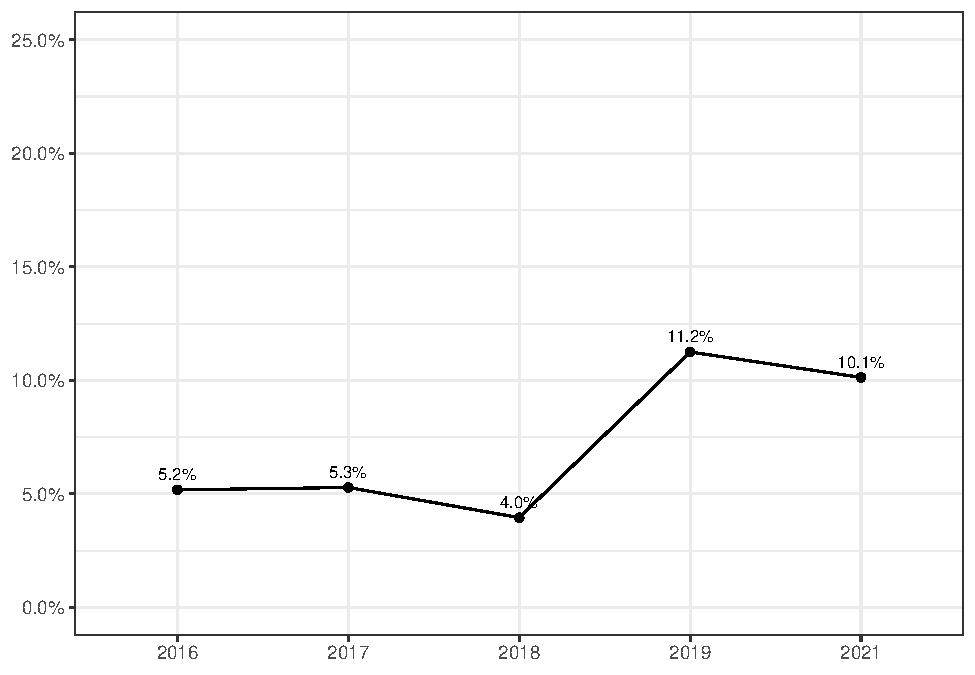
\includegraphics{reporte-elsoc_files/figure-latex/unnamed-chunk-13-1.pdf}

\hypertarget{confianza-en-instituciones}{%
\section{Confianza en instituciones}\label{confianza-en-instituciones}}

\hypertarget{bastante-o-mucha-confianza-en-ella-presidentea-de-la-repuxfablica-el-gobierno-y-el-congreso-nacional-seguxfan-auxf1o}{%
\subsection{1.9 Bastante o Mucha confianza en el/la Presidente(a) de la República, el Gobierno y el Congreso Nacional según año}\label{bastante-o-mucha-confianza-en-ella-presidentea-de-la-repuxfablica-el-gobierno-y-el-congreso-nacional-seguxfan-auxf1o}}

\begin{Shaded}
\begin{Highlighting}[]
\NormalTok{elsoc\_long\_2016\_2021 }\SpecialCharTok{\%\textgreater{}\%} 
  \FunctionTok{filter}\NormalTok{(tipo\_atricion }\SpecialCharTok{==} \DecValTok{1} \SpecialCharTok{\&} \SpecialCharTok{!}\NormalTok{c05\_01 }\SpecialCharTok{\%in\%} \FunctionTok{c}\NormalTok{(}\SpecialCharTok{{-}}\DecValTok{888}\NormalTok{, }\SpecialCharTok{{-}}\DecValTok{999}\NormalTok{) }\SpecialCharTok{\&} \SpecialCharTok{!}\NormalTok{c05\_07 }\SpecialCharTok{\%in\%} \FunctionTok{c}\NormalTok{(}\SpecialCharTok{{-}}\DecValTok{888}\NormalTok{, }\SpecialCharTok{{-}}\DecValTok{999}\NormalTok{) }\SpecialCharTok{\&} \SpecialCharTok{!}\NormalTok{c05\_08 }\SpecialCharTok{\%in\%} \FunctionTok{c}\NormalTok{(}\SpecialCharTok{{-}}\DecValTok{888}\NormalTok{, }\SpecialCharTok{{-}}\DecValTok{999}\NormalTok{)) }\SpecialCharTok{\%\textgreater{}\%} 
  \FunctionTok{pivot\_longer}\NormalTok{(}\AttributeTok{cols =} \FunctionTok{c}\NormalTok{(c05\_01, c05\_07, c05\_08)) }\SpecialCharTok{\%\textgreater{}\%} 
  \FunctionTok{prop}\NormalTok{(value }\SpecialCharTok{\%in\%} \DecValTok{4}\SpecialCharTok{:}\DecValTok{5}\NormalTok{, }\AttributeTok{by =} \FunctionTok{c}\NormalTok{(ola, name), }\AttributeTok{na.rm =} \ConstantTok{TRUE}\NormalTok{) }\SpecialCharTok{\%\textgreater{}\%} 
  \FunctionTok{as\_label}\NormalTok{(ola) }\SpecialCharTok{\%\textgreater{}\%} 
  \FunctionTok{mutate}\NormalTok{(}\AttributeTok{name =} \FunctionTok{factor}\NormalTok{(name, }
                       \AttributeTok{levels =} \FunctionTok{c}\NormalTok{(}\StringTok{\textquotesingle{}c05\_01\textquotesingle{}}\NormalTok{, }\StringTok{\textquotesingle{}c05\_07\textquotesingle{}}\NormalTok{, }\StringTok{\textquotesingle{}c05\_08\textquotesingle{}}\NormalTok{),}
                       \AttributeTok{labels =} \FunctionTok{c}\NormalTok{(}\StringTok{\textquotesingle{}Presidente/a de la Republica\textquotesingle{}}\NormalTok{, }\StringTok{\textquotesingle{}Congreso Nacional\textquotesingle{}}\NormalTok{, }\StringTok{\textquotesingle{}Gobierno de Chile\textquotesingle{}}\NormalTok{))) }\SpecialCharTok{\%\textgreater{}\%} 
  \FunctionTok{ggplot}\NormalTok{(}\FunctionTok{aes}\NormalTok{(}\AttributeTok{y =}\NormalTok{ prop, }\AttributeTok{x =}\NormalTok{ ola, }\AttributeTok{color =}\NormalTok{ name, }\AttributeTok{group =}\NormalTok{ name,}
               \AttributeTok{label =}\NormalTok{ scales}\SpecialCharTok{::}\FunctionTok{percent}\NormalTok{(prop, }\AttributeTok{accuracy =}\NormalTok{ .}\DecValTok{1}\NormalTok{))) }\SpecialCharTok{+}
    \FunctionTok{theme\_bw}\NormalTok{() }\SpecialCharTok{+}  
    \FunctionTok{geom\_line}\NormalTok{(}\AttributeTok{size =} \DecValTok{1}\NormalTok{) }\SpecialCharTok{+}
    \FunctionTok{geom\_point}\NormalTok{(}\AttributeTok{size =} \FloatTok{1.8}\NormalTok{) }\SpecialCharTok{+}
    \FunctionTok{scale\_y\_continuous}\NormalTok{(}\AttributeTok{labels =}\NormalTok{ scales}\SpecialCharTok{::}\NormalTok{percent,}
                       \AttributeTok{limits =} \FunctionTok{c}\NormalTok{(}\DecValTok{0}\NormalTok{,.}\DecValTok{5}\NormalTok{)) }\SpecialCharTok{+}
    \FunctionTok{ylab}\NormalTok{(}\AttributeTok{label =} \ConstantTok{NULL}\NormalTok{) }\SpecialCharTok{+}
    \FunctionTok{xlab}\NormalTok{(}\AttributeTok{label =} \ConstantTok{NULL}\NormalTok{) }\SpecialCharTok{+}
    \FunctionTok{scale\_color\_viridis\_d}\NormalTok{(}\AttributeTok{begin =}\NormalTok{ .}\DecValTok{1}\NormalTok{, }\AttributeTok{end =}\NormalTok{ .}\DecValTok{66}\NormalTok{, }\AttributeTok{option =} \StringTok{\textquotesingle{}viridis\textquotesingle{}}\NormalTok{) }\SpecialCharTok{+}
    \FunctionTok{geom\_text\_repel}\NormalTok{() }\SpecialCharTok{+}
    \FunctionTok{theme}\NormalTok{(}\AttributeTok{legend.position =} \StringTok{\textquotesingle{}top\textquotesingle{}}\NormalTok{,}
          \AttributeTok{legend.title =} \FunctionTok{element\_blank}\NormalTok{())}
\end{Highlighting}
\end{Shaded}

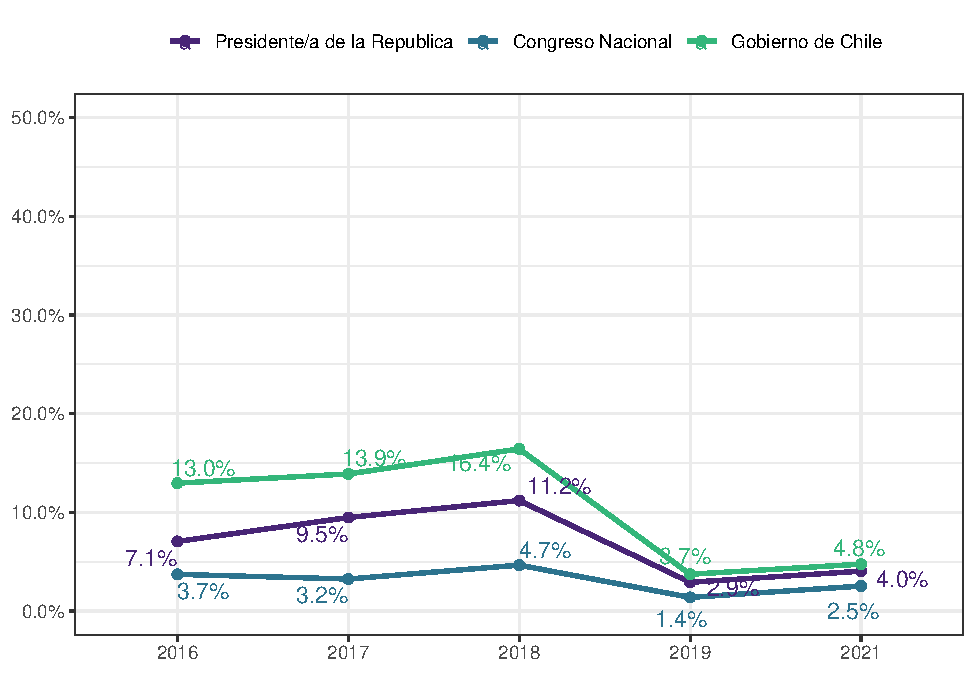
\includegraphics{reporte-elsoc_files/figure-latex/unnamed-chunk-14-1.pdf}

\hypertarget{bastante-o-mucha-confianza-en-carabineros-el-poder-judicial-y-en-partidos-poluxedticos-seguxfan-auxf1o}{%
\subsection{1.10 Bastante o Mucha confianza en Carabineros, el Poder Judicial y en Partidos Políticos según año}\label{bastante-o-mucha-confianza-en-carabineros-el-poder-judicial-y-en-partidos-poluxedticos-seguxfan-auxf1o}}

\begin{Shaded}
\begin{Highlighting}[]
\NormalTok{elsoc\_long\_2016\_2021 }\SpecialCharTok{\%\textgreater{}\%} 
  \FunctionTok{filter}\NormalTok{(tipo\_atricion }\SpecialCharTok{==} \DecValTok{1} \SpecialCharTok{\&} 
           \SpecialCharTok{!}\NormalTok{c05\_02 }\SpecialCharTok{\%in\%} \FunctionTok{c}\NormalTok{(}\SpecialCharTok{{-}}\DecValTok{888}\NormalTok{, }\SpecialCharTok{{-}}\DecValTok{999}\NormalTok{) }\SpecialCharTok{\&} \SpecialCharTok{!}\NormalTok{c05\_03 }\SpecialCharTok{\%in\%} \FunctionTok{c}\NormalTok{(}\SpecialCharTok{{-}}\DecValTok{888}\NormalTok{, }\SpecialCharTok{{-}}\DecValTok{999}\NormalTok{) }\SpecialCharTok{\&} \SpecialCharTok{!}\NormalTok{c05\_05 }\SpecialCharTok{\%in\%} \FunctionTok{c}\NormalTok{(}\SpecialCharTok{{-}}\DecValTok{888}\NormalTok{, }\SpecialCharTok{{-}}\DecValTok{999}\NormalTok{)) }\SpecialCharTok{\%\textgreater{}\%} 
  \FunctionTok{pivot\_longer}\NormalTok{(}\AttributeTok{cols =} \FunctionTok{c}\NormalTok{(c05\_02, c05\_03, c05\_05)) }\SpecialCharTok{\%\textgreater{}\%} 
  \FunctionTok{prop}\NormalTok{(value }\SpecialCharTok{\%in\%} \DecValTok{4}\SpecialCharTok{:}\DecValTok{5}\NormalTok{, }\AttributeTok{by =} \FunctionTok{c}\NormalTok{(ola, name), }\AttributeTok{na.rm =} \ConstantTok{TRUE}\NormalTok{) }\SpecialCharTok{\%\textgreater{}\%} 
  \FunctionTok{as\_label}\NormalTok{(ola) }\SpecialCharTok{\%\textgreater{}\%} 
  \FunctionTok{mutate}\NormalTok{(}\AttributeTok{name =} \FunctionTok{factor}\NormalTok{(name, }
                       \AttributeTok{levels =} \FunctionTok{c}\NormalTok{(}\StringTok{\textquotesingle{}c05\_02\textquotesingle{}}\NormalTok{, }\StringTok{\textquotesingle{}c05\_03\textquotesingle{}}\NormalTok{, }\StringTok{\textquotesingle{}c05\_05\textquotesingle{}}\NormalTok{),}
                       \AttributeTok{labels =} \FunctionTok{c}\NormalTok{(}\StringTok{\textquotesingle{}Partidos Políticos\textquotesingle{}}\NormalTok{, }
                                  \StringTok{\textquotesingle{}Carabineros de Chile\textquotesingle{}}\NormalTok{, }
                                  \StringTok{\textquotesingle{}Poder Judicial\textquotesingle{}}\NormalTok{))) }\SpecialCharTok{\%\textgreater{}\%}
  \FunctionTok{ggplot}\NormalTok{(}\FunctionTok{aes}\NormalTok{(}\AttributeTok{y =}\NormalTok{ prop, }\AttributeTok{x =}\NormalTok{ ola, }\AttributeTok{color =}\NormalTok{ name, }\AttributeTok{group =}\NormalTok{ name,}
               \AttributeTok{label =}\NormalTok{ scales}\SpecialCharTok{::}\FunctionTok{percent}\NormalTok{(prop, }\AttributeTok{accuracy =}\NormalTok{ .}\DecValTok{1}\NormalTok{))) }\SpecialCharTok{+}
    \FunctionTok{theme\_bw}\NormalTok{() }\SpecialCharTok{+}  
    \FunctionTok{geom\_line}\NormalTok{(}\AttributeTok{size =} \DecValTok{1}\NormalTok{) }\SpecialCharTok{+}
    \FunctionTok{geom\_point}\NormalTok{(}\AttributeTok{size =} \FloatTok{1.8}\NormalTok{) }\SpecialCharTok{+}
    \FunctionTok{scale\_y\_continuous}\NormalTok{(}\AttributeTok{labels =}\NormalTok{ scales}\SpecialCharTok{::}\NormalTok{percent,}
                       \AttributeTok{limits =} \FunctionTok{c}\NormalTok{(}\DecValTok{0}\NormalTok{,.}\DecValTok{5}\NormalTok{)) }\SpecialCharTok{+}
    \FunctionTok{ylab}\NormalTok{(}\AttributeTok{label =} \ConstantTok{NULL}\NormalTok{) }\SpecialCharTok{+}
    \FunctionTok{xlab}\NormalTok{(}\AttributeTok{label =} \ConstantTok{NULL}\NormalTok{) }\SpecialCharTok{+}
    \FunctionTok{scale\_color\_viridis\_d}\NormalTok{(}\AttributeTok{begin =}\NormalTok{ .}\DecValTok{1}\NormalTok{, }\AttributeTok{end =}\NormalTok{ .}\DecValTok{66}\NormalTok{, }\AttributeTok{option =} \StringTok{\textquotesingle{}viridis\textquotesingle{}}\NormalTok{) }\SpecialCharTok{+}
    \FunctionTok{geom\_text\_repel}\NormalTok{() }\SpecialCharTok{+}
    \FunctionTok{theme}\NormalTok{(}\AttributeTok{legend.position =} \StringTok{\textquotesingle{}top\textquotesingle{}}\NormalTok{,}
          \AttributeTok{legend.title =} \FunctionTok{element\_blank}\NormalTok{())}
\end{Highlighting}
\end{Shaded}

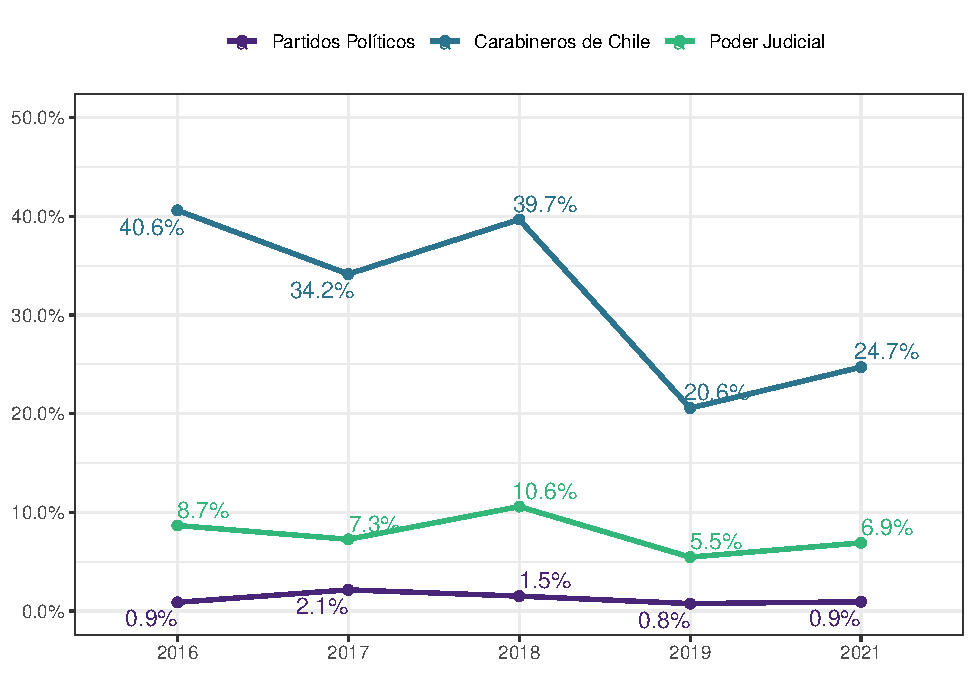
\includegraphics{reporte-elsoc_files/figure-latex/unnamed-chunk-15-1.pdf}

\hypertarget{identificaciuxf3n-poluxedtica}{%
\chapter{Identificación Política}\label{identificaciuxf3n-poluxedtica}}

\hypertarget{identificaciuxf3n-poluxedtica-1}{%
\section{Identificación política}\label{identificaciuxf3n-poluxedtica-1}}

\hypertarget{identificaciuxf3n-poluxedtica-por-ola}{%
\subsection{2.1 Identificación política por ola}\label{identificaciuxf3n-poluxedtica-por-ola}}

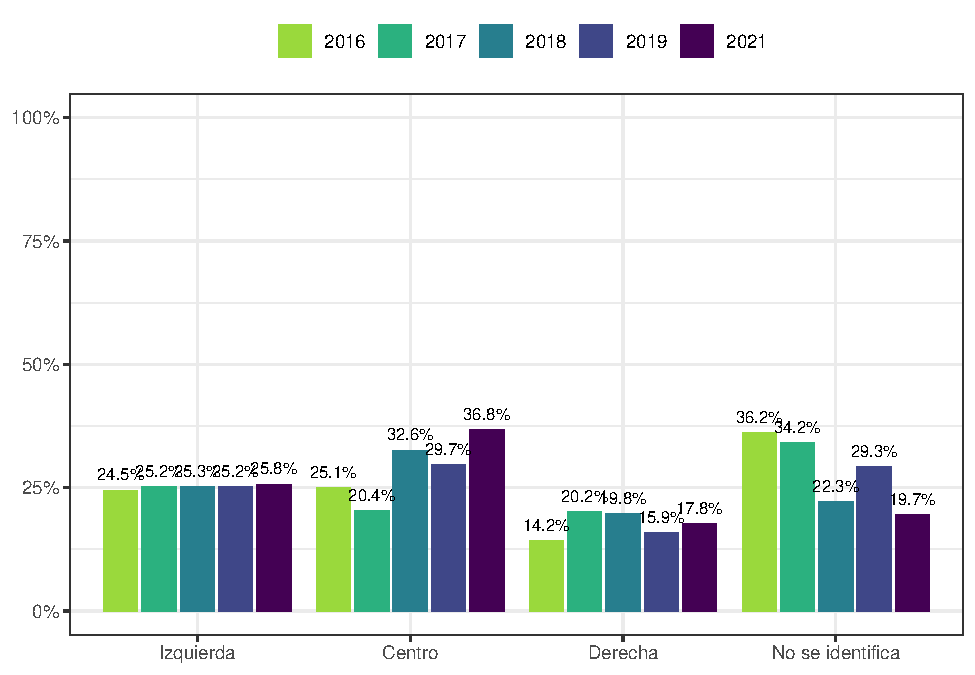
\includegraphics{reporte-elsoc_files/figure-latex/unnamed-chunk-16-1.pdf}

\hypertarget{alluvial-de-cambios-de-identificaciuxf3n-poluxedtica}{%
\subsection{2.2 Alluvial de cambios de Identificación política}\label{alluvial-de-cambios-de-identificaciuxf3n-poluxedtica}}

\hypertarget{de-acuerdo-o-totalmente-de-acuerdo-con-la-cuarentena-seguxfan-identificaciuxf3n-poluxedtica-el-auxf1o-2021}{%
\subsection{2.3 De acuerdo o Totalmente de acuerdo con la cuarentena según identificación política el año 2021}\label{de-acuerdo-o-totalmente-de-acuerdo-con-la-cuarentena-seguxfan-identificaciuxf3n-poluxedtica-el-auxf1o-2021}}

\begin{Shaded}
\begin{Highlighting}[]
\NormalTok{elsoc\_long\_2016\_2021 }\SpecialCharTok{\%\textgreater{}\%} 
  \FunctionTok{filter}\NormalTok{(ola }\SpecialCharTok{==} \DecValTok{5} \SpecialCharTok{\&}\NormalTok{ tipo\_atricion }\SpecialCharTok{==} \DecValTok{1} \SpecialCharTok{\&} 
           \SpecialCharTok{!}\NormalTok{c37\_10 }\SpecialCharTok{\%in\%} \FunctionTok{c}\NormalTok{(}\SpecialCharTok{{-}}\DecValTok{888}\NormalTok{, }\SpecialCharTok{{-}}\DecValTok{999}\NormalTok{) }\SpecialCharTok{\&} \SpecialCharTok{!}\NormalTok{c15 }\SpecialCharTok{\%in\%} \FunctionTok{c}\NormalTok{(}\SpecialCharTok{{-}}\DecValTok{888}\NormalTok{, }\SpecialCharTok{{-}}\DecValTok{999}\NormalTok{)) }\SpecialCharTok{\%\textgreater{}\%} 
    \FunctionTok{mutate}\NormalTok{(}\AttributeTok{pos\_id =} \FunctionTok{factor}\NormalTok{(car}\SpecialCharTok{::}\FunctionTok{recode}\NormalTok{(c15, }\AttributeTok{recodes =} \StringTok{"0:4 = 1; 5 = 2; 6:10 = 3; 11:12 = 4"}\NormalTok{),}
                         \AttributeTok{levels =} \FunctionTok{c}\NormalTok{(}\DecValTok{1}\NormalTok{, }\DecValTok{2}\NormalTok{, }\DecValTok{3}\NormalTok{, }\DecValTok{4}\NormalTok{),}
                         \AttributeTok{labels =} \FunctionTok{c}\NormalTok{(}\StringTok{\textquotesingle{}Izquierda\textquotesingle{}}\NormalTok{, }\StringTok{"Centro"}\NormalTok{, }\StringTok{"Derecha"}\NormalTok{, }\StringTok{"No se identifica"}\NormalTok{))) }\SpecialCharTok{\%\textgreater{}\%}
  \FunctionTok{prop}\NormalTok{(c37\_10 }\SpecialCharTok{\%in\%} \DecValTok{4}\SpecialCharTok{:}\DecValTok{5}\NormalTok{, pos\_id, }\AttributeTok{na.rm =} \ConstantTok{TRUE}\NormalTok{) }\SpecialCharTok{\%\textgreater{}\%} 
\NormalTok{  sjlabelled}\SpecialCharTok{::}\FunctionTok{as\_label}\NormalTok{(pos\_id) }\SpecialCharTok{\%\textgreater{}\%} 
  \FunctionTok{ggplot}\NormalTok{(}\FunctionTok{aes}\NormalTok{(}\AttributeTok{y =}\NormalTok{ prop, }\AttributeTok{x =}\NormalTok{ pos\_id, }\AttributeTok{fill =}\NormalTok{ pos\_id,}
               \AttributeTok{label =}\NormalTok{ scales}\SpecialCharTok{::}\FunctionTok{percent}\NormalTok{(prop, }\AttributeTok{accuracy =}\NormalTok{ .}\DecValTok{1}\NormalTok{))) }\SpecialCharTok{+}
  \FunctionTok{theme\_bw}\NormalTok{() }\SpecialCharTok{+} 
    \FunctionTok{geom\_col}\NormalTok{() }\SpecialCharTok{+}
    \FunctionTok{scale\_y\_continuous}\NormalTok{(}\AttributeTok{labels =}\NormalTok{ scales}\SpecialCharTok{::}\NormalTok{percent,}
                       \AttributeTok{limits =} \FunctionTok{c}\NormalTok{(}\DecValTok{0}\NormalTok{, }\DecValTok{1}\NormalTok{)) }\SpecialCharTok{+}
    \FunctionTok{ylab}\NormalTok{(}\AttributeTok{label =} \ConstantTok{NULL}\NormalTok{) }\SpecialCharTok{+}
    \FunctionTok{xlab}\NormalTok{(}\AttributeTok{label =} \ConstantTok{NULL}\NormalTok{) }\SpecialCharTok{+}
    \FunctionTok{scale\_fill\_viridis\_d}\NormalTok{(}\AttributeTok{begin =} \DecValTok{0}\NormalTok{, }\AttributeTok{end =}\NormalTok{ .}\DecValTok{85}\NormalTok{, }\AttributeTok{direction =} \SpecialCharTok{{-}}\DecValTok{1}\NormalTok{, }\AttributeTok{option =} \StringTok{\textquotesingle{}viridis\textquotesingle{}}\NormalTok{) }\SpecialCharTok{+}
    \FunctionTok{geom\_text}\NormalTok{(}\AttributeTok{vjust =} \SpecialCharTok{{-}}\FloatTok{0.8}\NormalTok{,}
              \AttributeTok{position =} \FunctionTok{position\_dodge}\NormalTok{(}\AttributeTok{width =}\NormalTok{ .}\DecValTok{9}\NormalTok{),}
              \AttributeTok{size=} \FloatTok{2.75}\NormalTok{) }\SpecialCharTok{+}
    \FunctionTok{theme}\NormalTok{(}\AttributeTok{legend.position =} \StringTok{\textquotesingle{}none\textquotesingle{}}\NormalTok{,   }
          \AttributeTok{legend.title =} \FunctionTok{element\_blank}\NormalTok{())}
\end{Highlighting}
\end{Shaded}

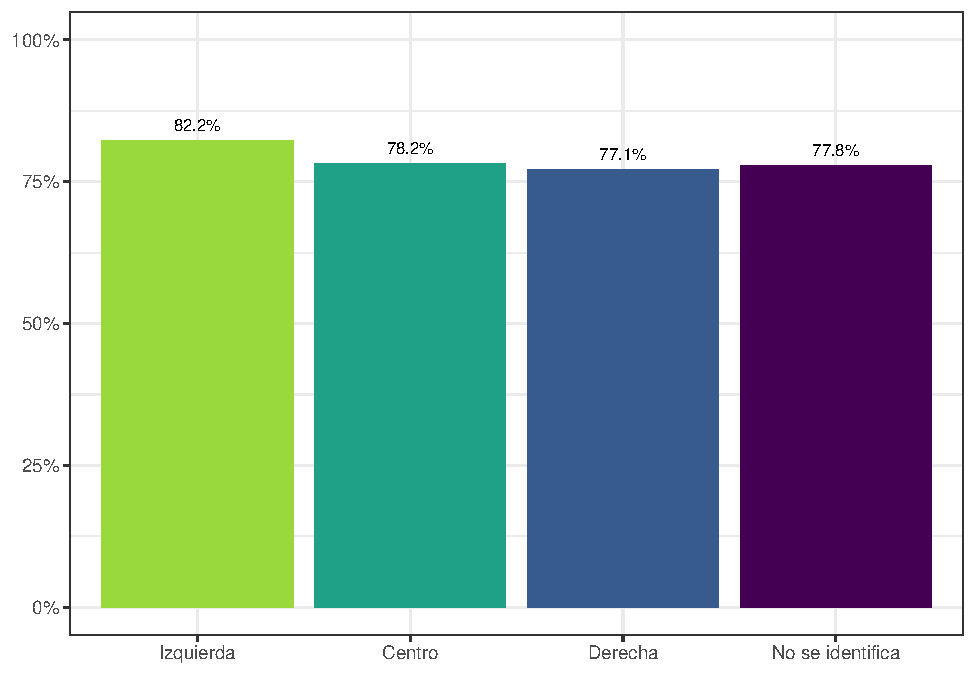
\includegraphics{reporte-elsoc_files/figure-latex/unnamed-chunk-18-1.pdf}

\hypertarget{grado-de-acuerdo-con-actividad-econuxf3mica-versus-salud-puxfablica-seguxfan-identificaciuxf3n-poluxedtica-el-auxf1o-2021}{%
\subsection{2.4 Grado de acuerdo con actividad económica versus salud pública según identificación política el año 2021}\label{grado-de-acuerdo-con-actividad-econuxf3mica-versus-salud-puxfablica-seguxfan-identificaciuxf3n-poluxedtica-el-auxf1o-2021}}

\begin{Shaded}
\begin{Highlighting}[]
\NormalTok{elsoc\_long\_2016\_2021 }\SpecialCharTok{\%\textgreater{}\%} 
  \FunctionTok{filter}\NormalTok{(ola }\SpecialCharTok{==} \DecValTok{5} \SpecialCharTok{\&}\NormalTok{ tipo\_atricion }\SpecialCharTok{==} \DecValTok{1} \SpecialCharTok{\&} 
           \SpecialCharTok{!}\NormalTok{c37\_09 }\SpecialCharTok{\%in\%} \FunctionTok{c}\NormalTok{(}\SpecialCharTok{{-}}\DecValTok{888}\NormalTok{, }\SpecialCharTok{{-}}\DecValTok{999}\NormalTok{) }\SpecialCharTok{\&} \SpecialCharTok{!}\NormalTok{c15 }\SpecialCharTok{\%in\%} \FunctionTok{c}\NormalTok{(}\SpecialCharTok{{-}}\DecValTok{888}\NormalTok{, }\SpecialCharTok{{-}}\DecValTok{999}\NormalTok{)) }\SpecialCharTok{\%\textgreater{}\%} 
    \FunctionTok{mutate}\NormalTok{(}\AttributeTok{pos\_id =} \FunctionTok{factor}\NormalTok{(car}\SpecialCharTok{::}\FunctionTok{recode}\NormalTok{(c15, }\AttributeTok{recodes =} \StringTok{"0:4 = 1; 5 = 2; 6:10 = 3; 11:12 = 4"}\NormalTok{),}
                         \AttributeTok{levels =} \FunctionTok{c}\NormalTok{(}\DecValTok{1}\NormalTok{, }\DecValTok{2}\NormalTok{, }\DecValTok{3}\NormalTok{, }\DecValTok{4}\NormalTok{),}
                         \AttributeTok{labels =} \FunctionTok{c}\NormalTok{(}\StringTok{\textquotesingle{}Izquierda\textquotesingle{}}\NormalTok{, }\StringTok{"Centro"}\NormalTok{, }\StringTok{"Derecha"}\NormalTok{, }\StringTok{"No se identifica"}\NormalTok{))) }\SpecialCharTok{\%\textgreater{}\%}
  \FunctionTok{prop}\NormalTok{(c37\_09 }\SpecialCharTok{\%in\%} \DecValTok{4}\SpecialCharTok{:}\DecValTok{5}\NormalTok{, pos\_id, }\AttributeTok{na.rm =} \ConstantTok{TRUE}\NormalTok{) }\SpecialCharTok{\%\textgreater{}\%} 
\NormalTok{  sjlabelled}\SpecialCharTok{::}\FunctionTok{as\_label}\NormalTok{(c37\_09, pos\_id) }\SpecialCharTok{\%\textgreater{}\%} 
  \FunctionTok{ggplot}\NormalTok{(}\FunctionTok{aes}\NormalTok{(}\AttributeTok{y =}\NormalTok{ prop, }\AttributeTok{x =}\NormalTok{ pos\_id, }\AttributeTok{fill =}\NormalTok{ pos\_id, }
               \AttributeTok{label =}\NormalTok{ scales}\SpecialCharTok{::}\FunctionTok{percent}\NormalTok{(prop, }\AttributeTok{accuracy =}\NormalTok{ .}\DecValTok{1}\NormalTok{))) }\SpecialCharTok{+}
  \FunctionTok{theme\_bw}\NormalTok{() }\SpecialCharTok{+} 
    \FunctionTok{geom\_col}\NormalTok{() }\SpecialCharTok{+}
    \FunctionTok{scale\_y\_continuous}\NormalTok{(}\AttributeTok{labels =}\NormalTok{ scales}\SpecialCharTok{::}\NormalTok{percent, }\AttributeTok{limits =} \FunctionTok{c}\NormalTok{(}\DecValTok{0}\NormalTok{,}\DecValTok{1}\NormalTok{)) }\SpecialCharTok{+} 
    \FunctionTok{ylab}\NormalTok{(}\AttributeTok{label =} \ConstantTok{NULL}\NormalTok{) }\SpecialCharTok{+}
    \FunctionTok{xlab}\NormalTok{(}\AttributeTok{label =} \ConstantTok{NULL}\NormalTok{) }\SpecialCharTok{+}
    \FunctionTok{scale\_fill\_viridis\_d}\NormalTok{(}\AttributeTok{begin =} \DecValTok{0}\NormalTok{, }\AttributeTok{end =}\NormalTok{ .}\DecValTok{85}\NormalTok{, }\AttributeTok{direction =} \SpecialCharTok{{-}}\DecValTok{1}\NormalTok{, }\AttributeTok{option =} \StringTok{\textquotesingle{}viridis\textquotesingle{}}\NormalTok{) }\SpecialCharTok{+}
    \FunctionTok{geom\_text}\NormalTok{(}\AttributeTok{vjust =} \SpecialCharTok{{-}}\FloatTok{0.8}\NormalTok{,}
              \AttributeTok{position =} \FunctionTok{position\_dodge}\NormalTok{(}\AttributeTok{width =}\NormalTok{ .}\DecValTok{9}\NormalTok{),}
              \AttributeTok{size=} \FloatTok{2.75}\NormalTok{) }\SpecialCharTok{+}
    \FunctionTok{theme}\NormalTok{(}\AttributeTok{legend.position =} \StringTok{\textquotesingle{}none\textquotesingle{}}\NormalTok{,   }
          \AttributeTok{legend.title =} \FunctionTok{element\_blank}\NormalTok{())}
\end{Highlighting}
\end{Shaded}

\begin{verbatim}
## 1 variables were not found in the dataset: c37_09
\end{verbatim}

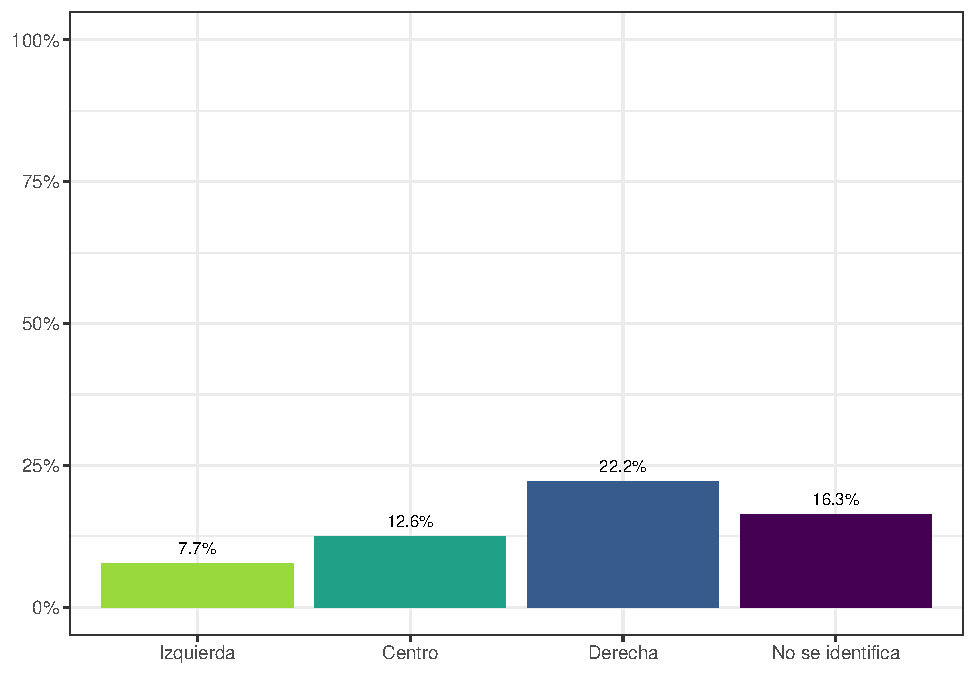
\includegraphics{reporte-elsoc_files/figure-latex/unnamed-chunk-19-1.pdf}

\hypertarget{grado-de-acuerdo-con-el-aborto-seguxfan-identificaciuxf3n-poluxedtica}{%
\subsection{2.6 Grado de acuerdo con el aborto según identificación política}\label{grado-de-acuerdo-con-el-aborto-seguxfan-identificaciuxf3n-poluxedtica}}

\begin{Shaded}
\begin{Highlighting}[]
\NormalTok{elsoc\_long\_2016\_2021 }\SpecialCharTok{\%\textgreater{}\%}
  \FunctionTok{filter}\NormalTok{(tipo\_atricion }\SpecialCharTok{==} \DecValTok{1} \SpecialCharTok{\&}\NormalTok{ ola }\SpecialCharTok{\%in\%} \DecValTok{3}\SpecialCharTok{:}\DecValTok{5} \SpecialCharTok{\&} \SpecialCharTok{!}\NormalTok{c37\_02 }\SpecialCharTok{\%in\%} \FunctionTok{c}\NormalTok{(}\SpecialCharTok{{-}}\DecValTok{888}\NormalTok{, }\SpecialCharTok{{-}}\DecValTok{999}\NormalTok{) }\SpecialCharTok{\&} \SpecialCharTok{!}\NormalTok{c15 }\SpecialCharTok{\%in\%} \FunctionTok{c}\NormalTok{(}\SpecialCharTok{{-}}\DecValTok{888}\NormalTok{, }\SpecialCharTok{{-}}\DecValTok{999}\NormalTok{)) }\SpecialCharTok{\%\textgreater{}\%}
  \FunctionTok{mutate}\NormalTok{(}\AttributeTok{pos\_id =} \FunctionTok{factor}\NormalTok{(car}\SpecialCharTok{::}\FunctionTok{recode}\NormalTok{(c15, }\AttributeTok{recodes =} \StringTok{"0:4 = 1; 5 = 2; 6:10 = 3; 11:12 = 4"}\NormalTok{),}
                         \AttributeTok{levels =} \FunctionTok{c}\NormalTok{(}\DecValTok{1}\NormalTok{, }\DecValTok{2}\NormalTok{, }\DecValTok{3}\NormalTok{, }\DecValTok{4}\NormalTok{),}
                         \AttributeTok{labels =} \FunctionTok{c}\NormalTok{(}\StringTok{\textquotesingle{}Izquierda\textquotesingle{}}\NormalTok{, }\StringTok{"Centro"}\NormalTok{, }\StringTok{"Derecha"}\NormalTok{, }\StringTok{"No se identifica"}\NormalTok{))) }\SpecialCharTok{\%\textgreater{}\%}
  \FunctionTok{prop}\NormalTok{(c37\_02 }\SpecialCharTok{\%in\%} \DecValTok{4}\SpecialCharTok{:}\DecValTok{5}\NormalTok{, }\AttributeTok{by =} \FunctionTok{c}\NormalTok{(ola, pos\_id), }\AttributeTok{na.rm =} \ConstantTok{TRUE}\NormalTok{) }\SpecialCharTok{\%\textgreater{}\%}
  \FunctionTok{as\_label}\NormalTok{(ola) }\SpecialCharTok{\%\textgreater{}\%} 
  \FunctionTok{ggplot}\NormalTok{(}\FunctionTok{aes}\NormalTok{(}\AttributeTok{y =}\NormalTok{ prop, }\AttributeTok{x =}\NormalTok{ pos\_id, }\AttributeTok{fill =}\NormalTok{ ola,  }
               \AttributeTok{label =}\NormalTok{ scales}\SpecialCharTok{::}\FunctionTok{percent}\NormalTok{(prop, }\AttributeTok{accuracy =}\NormalTok{ .}\DecValTok{1}\NormalTok{))) }\SpecialCharTok{+}
    \FunctionTok{theme\_bw}\NormalTok{() }\SpecialCharTok{+} 
    \FunctionTok{geom\_col}\NormalTok{(}\AttributeTok{position=} \StringTok{\textquotesingle{}dodge2\textquotesingle{}}\NormalTok{) }\SpecialCharTok{+}
    \FunctionTok{scale\_y\_continuous}\NormalTok{(}\AttributeTok{labels =}\NormalTok{ scales}\SpecialCharTok{::}\NormalTok{percent,}
                       \AttributeTok{limits =} \FunctionTok{c}\NormalTok{(}\DecValTok{0}\NormalTok{, }\DecValTok{1}\NormalTok{)) }\SpecialCharTok{+}
    \FunctionTok{ylab}\NormalTok{(}\AttributeTok{label =} \ConstantTok{NULL}\NormalTok{) }\SpecialCharTok{+}
    \FunctionTok{xlab}\NormalTok{(}\AttributeTok{label =} \ConstantTok{NULL}\NormalTok{) }\SpecialCharTok{+}
    \FunctionTok{scale\_fill\_viridis\_d}\NormalTok{(}\AttributeTok{begin =} \DecValTok{0}\NormalTok{, }\AttributeTok{end =}\NormalTok{ .}\DecValTok{85}\NormalTok{, }\AttributeTok{direction =} \SpecialCharTok{{-}}\DecValTok{1}\NormalTok{, }\AttributeTok{option =} \StringTok{\textquotesingle{}viridis\textquotesingle{}}\NormalTok{) }\SpecialCharTok{+}
    \FunctionTok{geom\_text}\NormalTok{(}\AttributeTok{vjust =} \SpecialCharTok{{-}}\FloatTok{0.8}\NormalTok{,}
              \AttributeTok{position =} \FunctionTok{position\_dodge}\NormalTok{(}\AttributeTok{width =}\NormalTok{ .}\DecValTok{9}\NormalTok{),}
              \AttributeTok{size=} \FloatTok{2.75}\NormalTok{) }\SpecialCharTok{+}
    \FunctionTok{theme}\NormalTok{(}\AttributeTok{legend.position =} \StringTok{\textquotesingle{}top\textquotesingle{}}\NormalTok{,}
          \AttributeTok{legend.title =} \FunctionTok{element\_blank}\NormalTok{())}
\end{Highlighting}
\end{Shaded}

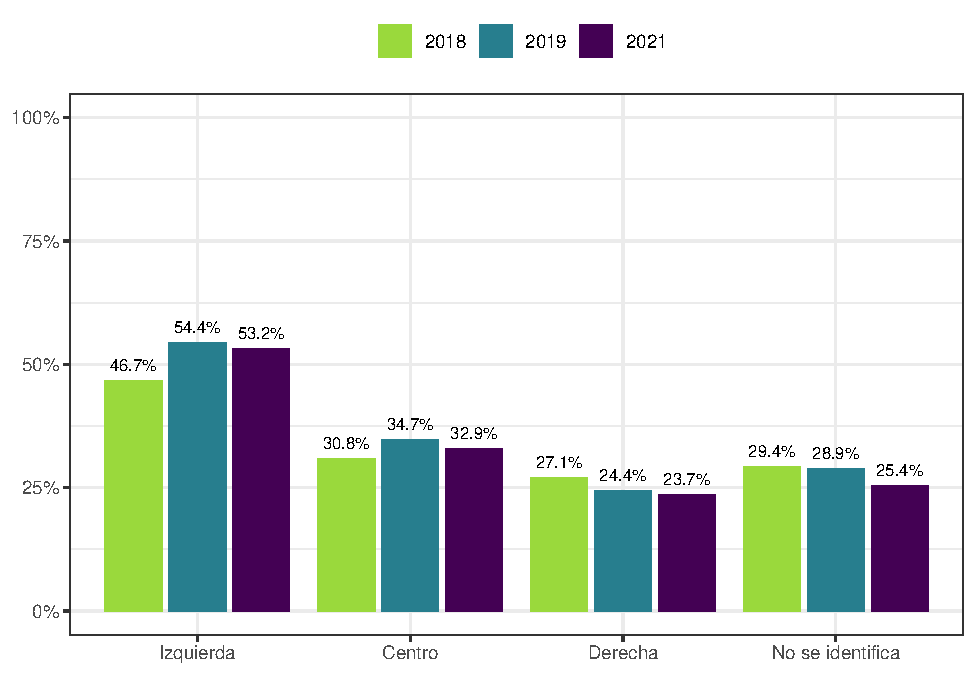
\includegraphics{reporte-elsoc_files/figure-latex/unnamed-chunk-20-1.pdf}

\hypertarget{grado-de-acuerdo-con-la-capitalizacion-individual-pensiones-seguxfan-identificaciuxf3n-poluxedtica}{%
\subsection{2.7 Grado de acuerdo con la capitalizacion individual pensiones según identificación política}\label{grado-de-acuerdo-con-la-capitalizacion-individual-pensiones-seguxfan-identificaciuxf3n-poluxedtica}}

\begin{Shaded}
\begin{Highlighting}[]
\NormalTok{elsoc\_long\_2016\_2021 }\SpecialCharTok{\%\textgreater{}\%}
  \FunctionTok{filter}\NormalTok{(tipo\_atricion }\SpecialCharTok{==} \DecValTok{1} \SpecialCharTok{\&}\NormalTok{ ola }\SpecialCharTok{\%in\%} \DecValTok{3}\SpecialCharTok{:}\DecValTok{5} \SpecialCharTok{\&} \SpecialCharTok{!}\NormalTok{c37\_02 }\SpecialCharTok{\%in\%} \FunctionTok{c}\NormalTok{(}\SpecialCharTok{{-}}\DecValTok{888}\NormalTok{, }\SpecialCharTok{{-}}\DecValTok{999}\NormalTok{) }\SpecialCharTok{\&} \SpecialCharTok{!}\NormalTok{c15 }\SpecialCharTok{\%in\%} \FunctionTok{c}\NormalTok{(}\SpecialCharTok{{-}}\DecValTok{888}\NormalTok{, }\SpecialCharTok{{-}}\DecValTok{999}\NormalTok{)) }\SpecialCharTok{\%\textgreater{}\%}
  \FunctionTok{mutate}\NormalTok{(}\AttributeTok{pos\_id =} \FunctionTok{factor}\NormalTok{(car}\SpecialCharTok{::}\FunctionTok{recode}\NormalTok{(c15, }\AttributeTok{recodes =} \StringTok{"0:4 = 1; 5 = 2; 6:10 = 3; 11:12 = 4"}\NormalTok{),}
                         \AttributeTok{levels =} \FunctionTok{c}\NormalTok{(}\DecValTok{1}\NormalTok{, }\DecValTok{2}\NormalTok{, }\DecValTok{3}\NormalTok{, }\DecValTok{4}\NormalTok{),}
                         \AttributeTok{labels =} \FunctionTok{c}\NormalTok{(}\StringTok{\textquotesingle{}Izquierda\textquotesingle{}}\NormalTok{, }\StringTok{"Centro"}\NormalTok{, }\StringTok{"Derecha"}\NormalTok{, }\StringTok{"No se identifica"}\NormalTok{))) }\SpecialCharTok{\%\textgreater{}\%}
  \FunctionTok{prop}\NormalTok{(c37\_02 }\SpecialCharTok{\%in\%} \DecValTok{4}\SpecialCharTok{:}\DecValTok{5}\NormalTok{, }\AttributeTok{by =} \FunctionTok{c}\NormalTok{(ola, pos\_id), }\AttributeTok{na.rm =} \ConstantTok{TRUE}\NormalTok{) }\SpecialCharTok{\%\textgreater{}\%}
  \FunctionTok{as\_label}\NormalTok{(ola) }\SpecialCharTok{\%\textgreater{}\%} 
  \FunctionTok{ggplot}\NormalTok{(}\FunctionTok{aes}\NormalTok{(}\AttributeTok{y =}\NormalTok{ prop, }\AttributeTok{x =}\NormalTok{ pos\_id, }\AttributeTok{fill =}\NormalTok{ ola,  }
               \AttributeTok{label =}\NormalTok{ scales}\SpecialCharTok{::}\FunctionTok{percent}\NormalTok{(prop, }\AttributeTok{accuracy =}\NormalTok{ .}\DecValTok{1}\NormalTok{))) }\SpecialCharTok{+}
    \FunctionTok{theme\_bw}\NormalTok{() }\SpecialCharTok{+} 
    \FunctionTok{geom\_col}\NormalTok{(}\AttributeTok{position=} \StringTok{\textquotesingle{}dodge2\textquotesingle{}}\NormalTok{) }\SpecialCharTok{+}
    \FunctionTok{scale\_y\_continuous}\NormalTok{(}\AttributeTok{labels =}\NormalTok{ scales}\SpecialCharTok{::}\NormalTok{percent,}
                       \AttributeTok{limits =} \FunctionTok{c}\NormalTok{(}\DecValTok{0}\NormalTok{, }\DecValTok{1}\NormalTok{)) }\SpecialCharTok{+}
    \FunctionTok{ylab}\NormalTok{(}\AttributeTok{label =} \ConstantTok{NULL}\NormalTok{) }\SpecialCharTok{+}
    \FunctionTok{xlab}\NormalTok{(}\AttributeTok{label =} \ConstantTok{NULL}\NormalTok{) }\SpecialCharTok{+}
    \FunctionTok{scale\_fill\_viridis\_d}\NormalTok{(}\AttributeTok{begin =} \DecValTok{0}\NormalTok{, }\AttributeTok{end =}\NormalTok{ .}\DecValTok{85}\NormalTok{, }\AttributeTok{direction =} \SpecialCharTok{{-}}\DecValTok{1}\NormalTok{, }\AttributeTok{option =} \StringTok{\textquotesingle{}viridis\textquotesingle{}}\NormalTok{) }\SpecialCharTok{+}
    \FunctionTok{geom\_text}\NormalTok{(}\AttributeTok{vjust =} \SpecialCharTok{{-}}\FloatTok{0.8}\NormalTok{,}
              \AttributeTok{position =} \FunctionTok{position\_dodge}\NormalTok{(}\AttributeTok{width =}\NormalTok{ .}\DecValTok{9}\NormalTok{),}
              \AttributeTok{size=} \FloatTok{2.75}\NormalTok{) }\SpecialCharTok{+}
    \FunctionTok{theme}\NormalTok{(}\AttributeTok{legend.position =} \StringTok{\textquotesingle{}top\textquotesingle{}}\NormalTok{,}
          \AttributeTok{legend.title =} \FunctionTok{element\_blank}\NormalTok{())}
\end{Highlighting}
\end{Shaded}

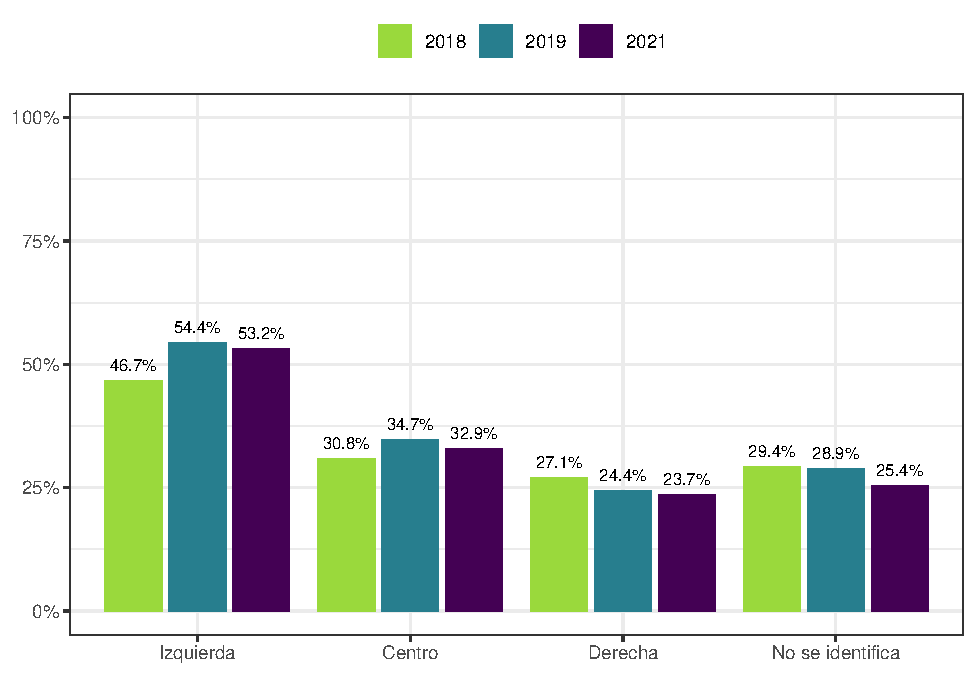
\includegraphics{reporte-elsoc_files/figure-latex/unnamed-chunk-21-1.pdf}

\hypertarget{grado-de-acuerdo-con-las-restricciones-de-ingreso-de-migrantes-seguxfan-identificaciuxf3n-poluxedtica-2019}{%
\subsection{2.8 Grado de acuerdo con las restricciones de ingreso de migrantes según identificación política (2019)}\label{grado-de-acuerdo-con-las-restricciones-de-ingreso-de-migrantes-seguxfan-identificaciuxf3n-poluxedtica-2019}}

\begin{Shaded}
\begin{Highlighting}[]
\NormalTok{elsoc\_long\_2016\_2021 }\SpecialCharTok{\%\textgreater{}\%}
  \FunctionTok{filter}\NormalTok{(tipo\_atricion }\SpecialCharTok{==} \DecValTok{1} \SpecialCharTok{\&}\NormalTok{ ola }\SpecialCharTok{\%in\%} \DecValTok{3}\SpecialCharTok{:}\DecValTok{5} \SpecialCharTok{\&} 
           \SpecialCharTok{!}\NormalTok{c37\_05 }\SpecialCharTok{\%in\%} \FunctionTok{c}\NormalTok{(}\SpecialCharTok{{-}}\DecValTok{888}\NormalTok{, }\SpecialCharTok{{-}}\DecValTok{999}\NormalTok{) }\SpecialCharTok{\&} \SpecialCharTok{!}\NormalTok{c15 }\SpecialCharTok{\%in\%} \FunctionTok{c}\NormalTok{(}\SpecialCharTok{{-}}\DecValTok{888}\NormalTok{, }\SpecialCharTok{{-}}\DecValTok{999}\NormalTok{)) }\SpecialCharTok{\%\textgreater{}\%}
    \FunctionTok{mutate}\NormalTok{(}\AttributeTok{pos\_id =} \FunctionTok{factor}\NormalTok{(car}\SpecialCharTok{::}\FunctionTok{recode}\NormalTok{(c15, }\AttributeTok{recodes =} \StringTok{"0:4 = 1; 5 = 2; 6:10 = 3; 11:12 = 4"}\NormalTok{),}
                         \AttributeTok{levels =} \FunctionTok{c}\NormalTok{(}\DecValTok{1}\NormalTok{, }\DecValTok{2}\NormalTok{, }\DecValTok{3}\NormalTok{, }\DecValTok{4}\NormalTok{),}
                         \AttributeTok{labels =} \FunctionTok{c}\NormalTok{(}\StringTok{\textquotesingle{}Izquierda\textquotesingle{}}\NormalTok{, }\StringTok{"Centro"}\NormalTok{, }\StringTok{"Derecha"}\NormalTok{, }\StringTok{"No se identifica"}\NormalTok{))) }\SpecialCharTok{\%\textgreater{}\%}
  \FunctionTok{prop}\NormalTok{(}\AttributeTok{x =}\NormalTok{ c37\_05 }\SpecialCharTok{\%in\%} \DecValTok{4}\SpecialCharTok{:}\DecValTok{5}\NormalTok{, }\AttributeTok{by =} \FunctionTok{c}\NormalTok{(ola, pos\_id), }\AttributeTok{na.rm =} \ConstantTok{TRUE}\NormalTok{) }\SpecialCharTok{\%\textgreater{}\%} 
  \FunctionTok{as\_label}\NormalTok{(ola) }\SpecialCharTok{\%\textgreater{}\%} 
  \FunctionTok{ggplot}\NormalTok{(}\FunctionTok{aes}\NormalTok{(}\AttributeTok{y =}\NormalTok{ prop, }\AttributeTok{x =}\NormalTok{ pos\_id, }\AttributeTok{fill =}\NormalTok{ ola, }
               \AttributeTok{label =}\NormalTok{ scales}\SpecialCharTok{::}\FunctionTok{percent}\NormalTok{(prop, }\AttributeTok{accuracy =}\NormalTok{ .}\DecValTok{1}\NormalTok{))) }\SpecialCharTok{+}
    \FunctionTok{theme\_bw}\NormalTok{() }\SpecialCharTok{+} 
    \FunctionTok{geom\_col}\NormalTok{(}\AttributeTok{position=} \StringTok{\textquotesingle{}dodge2\textquotesingle{}}\NormalTok{) }\SpecialCharTok{+}
    \FunctionTok{scale\_y\_continuous}\NormalTok{(}\AttributeTok{labels =}\NormalTok{ scales}\SpecialCharTok{::}\NormalTok{percent,}
                       \AttributeTok{limits =} \FunctionTok{c}\NormalTok{(}\DecValTok{0}\NormalTok{, }\DecValTok{1}\NormalTok{)) }\SpecialCharTok{+}
    \FunctionTok{ylab}\NormalTok{(}\AttributeTok{label =} \ConstantTok{NULL}\NormalTok{) }\SpecialCharTok{+}
    \FunctionTok{xlab}\NormalTok{(}\AttributeTok{label =} \ConstantTok{NULL}\NormalTok{) }\SpecialCharTok{+}
    \FunctionTok{scale\_fill\_viridis\_d}\NormalTok{(}\AttributeTok{begin =} \DecValTok{0}\NormalTok{, }\AttributeTok{end =}\NormalTok{ .}\DecValTok{85}\NormalTok{, }\AttributeTok{direction =} \SpecialCharTok{{-}}\DecValTok{1}\NormalTok{, }\AttributeTok{option =} \StringTok{\textquotesingle{}viridis\textquotesingle{}}\NormalTok{) }\SpecialCharTok{+}
    \FunctionTok{geom\_text}\NormalTok{(}\AttributeTok{vjust =} \SpecialCharTok{{-}}\FloatTok{0.8}\NormalTok{,}
              \AttributeTok{position =} \FunctionTok{position\_dodge}\NormalTok{(}\AttributeTok{width =}\NormalTok{ .}\DecValTok{9}\NormalTok{),}
              \AttributeTok{size=} \FloatTok{2.75}\NormalTok{) }\SpecialCharTok{+}
    \FunctionTok{theme}\NormalTok{(}\AttributeTok{legend.position =} \StringTok{\textquotesingle{}top\textquotesingle{}}\NormalTok{,}
          \AttributeTok{legend.title =} \FunctionTok{element\_blank}\NormalTok{())}
\end{Highlighting}
\end{Shaded}

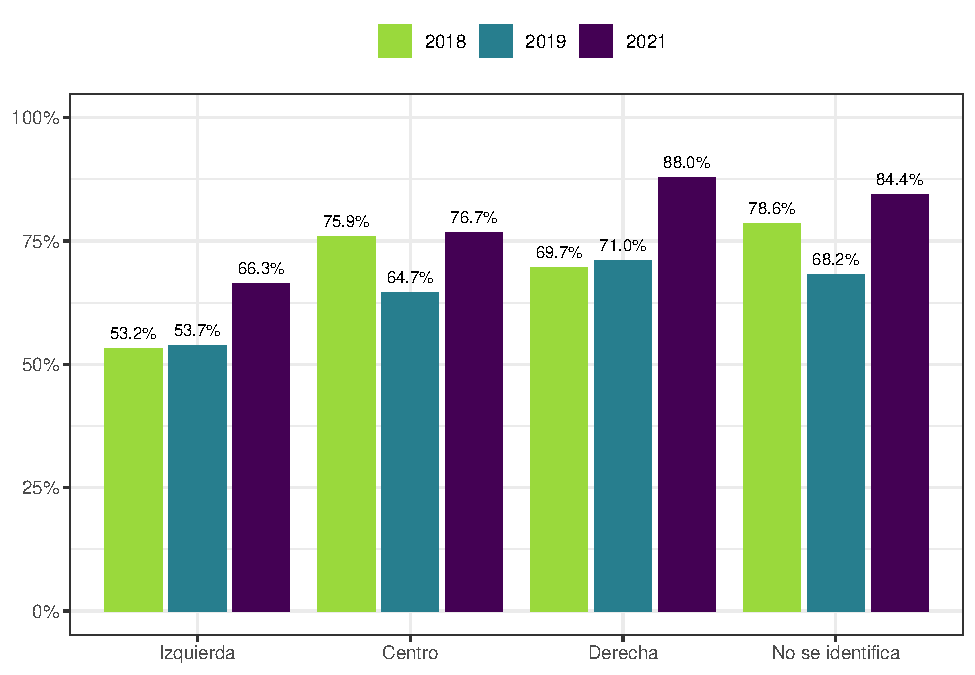
\includegraphics{reporte-elsoc_files/figure-latex/unnamed-chunk-22-1.pdf}

\hypertarget{actitudes-hacia-la-democracia}{%
\chapter{Actitudes hacia la democracia}\label{actitudes-hacia-la-democracia}}

\hypertarget{apoyo-a-la-democracia}{%
\section{Apoyo a la Democracia}\label{apoyo-a-la-democracia}}

\hypertarget{con-cuuxe1l-de-las-siguientes-frases-estuxe1-usted-muxe1s-de-acuerdo}{%
\subsection{3.1 ¿Con cuál de las siguientes frases está usted más de acuerdo?}\label{con-cuuxe1l-de-las-siguientes-frases-estuxe1-usted-muxe1s-de-acuerdo}}

\hypertarget{insatisfacciuxf3n-con-la-democracia-por-ola}{%
\subsection{3.2 Insatisfacción con la democracia por ola}\label{insatisfacciuxf3n-con-la-democracia-por-ola}}

\begin{Shaded}
\begin{Highlighting}[]
\NormalTok{datos.}\FloatTok{3.2} \OtherTok{\textless{}{-}}\NormalTok{ elsoc\_long\_2016\_2021 }\SpecialCharTok{\%\textgreater{}\%}
  \FunctionTok{filter}\NormalTok{(tipo\_atricion }\SpecialCharTok{==} \DecValTok{1} \SpecialCharTok{\&} \SpecialCharTok{!}\NormalTok{c01 }\SpecialCharTok{\%in\%} \FunctionTok{c}\NormalTok{(}\SpecialCharTok{{-}}\DecValTok{999}\NormalTok{,}\SpecialCharTok{{-}}\DecValTok{888}\NormalTok{)) }\SpecialCharTok{\%\textgreater{}\%}
  \FunctionTok{prop}\NormalTok{(c01 }\SpecialCharTok{\%in\%} \FunctionTok{c}\NormalTok{(}\DecValTok{1}\NormalTok{), }\AttributeTok{by  =} \FunctionTok{c}\NormalTok{(ola), }\AttributeTok{na.rm =} \ConstantTok{TRUE}\NormalTok{) }\SpecialCharTok{\%\textgreater{}\%}
\NormalTok{  sjlabelled}\SpecialCharTok{::}\FunctionTok{as\_label}\NormalTok{(ola, c01)}
\end{Highlighting}
\end{Shaded}

\begin{verbatim}
## 1 variables were not found in the dataset: c01
\end{verbatim}

\begin{Shaded}
\begin{Highlighting}[]
\NormalTok{g.}\FloatTok{3.2} \OtherTok{\textless{}{-}}\NormalTok{ datos.}\FloatTok{3.2} \SpecialCharTok{\%\textgreater{}\%} 
  \FunctionTok{ggplot}\NormalTok{(}\FunctionTok{aes}\NormalTok{(}\AttributeTok{y =}\NormalTok{ prop, }\AttributeTok{x =}\NormalTok{ ola, }\AttributeTok{group =} \DecValTok{1}\NormalTok{,}
               \AttributeTok{label =}\NormalTok{ scales}\SpecialCharTok{::}\FunctionTok{percent}\NormalTok{(prop, }\AttributeTok{accuracy =}\NormalTok{ .}\DecValTok{1}\NormalTok{))) }\SpecialCharTok{+}
  \FunctionTok{theme\_bw}\NormalTok{() }\SpecialCharTok{+} 
  \FunctionTok{geom\_point}\NormalTok{() }\SpecialCharTok{+}
  \FunctionTok{geom\_line}\NormalTok{() }\SpecialCharTok{+} 
  \FunctionTok{scale\_y\_continuous}\NormalTok{(}\AttributeTok{labels =}\NormalTok{ scales}\SpecialCharTok{::}\NormalTok{percent,}
                     \AttributeTok{limits =} \FunctionTok{c}\NormalTok{(}\DecValTok{0}\NormalTok{, }\DecValTok{1}\NormalTok{)) }\SpecialCharTok{+}
  \FunctionTok{ylab}\NormalTok{(}\AttributeTok{label =} \ConstantTok{NULL}\NormalTok{) }\SpecialCharTok{+}
  \FunctionTok{xlab}\NormalTok{(}\AttributeTok{label =} \ConstantTok{NULL}\NormalTok{) }\SpecialCharTok{+}
  \FunctionTok{scale\_fill\_viridis\_d}\NormalTok{(}\AttributeTok{begin =} \DecValTok{0}\NormalTok{, }\AttributeTok{end =}\NormalTok{ .}\DecValTok{85}\NormalTok{, }\AttributeTok{direction =} \SpecialCharTok{{-}}\DecValTok{1}\NormalTok{, }\AttributeTok{option =} \StringTok{\textquotesingle{}viridis\textquotesingle{}}\NormalTok{) }\SpecialCharTok{+}
  \FunctionTok{geom\_text}\NormalTok{(}\AttributeTok{vjust =} \SpecialCharTok{{-}}\FloatTok{0.8}\NormalTok{,}
            \AttributeTok{position =} \FunctionTok{position\_dodge}\NormalTok{(}\AttributeTok{width =}\NormalTok{ .}\DecValTok{9}\NormalTok{),}
            \AttributeTok{size=} \FloatTok{2.75}\NormalTok{) }\SpecialCharTok{+}
  \FunctionTok{theme}\NormalTok{(}\AttributeTok{legend.position =} \StringTok{\textquotesingle{}none\textquotesingle{}}\NormalTok{,   }
        \AttributeTok{legend.title =} \FunctionTok{element\_blank}\NormalTok{())}
\NormalTok{g.}\FloatTok{3.2}
\end{Highlighting}
\end{Shaded}

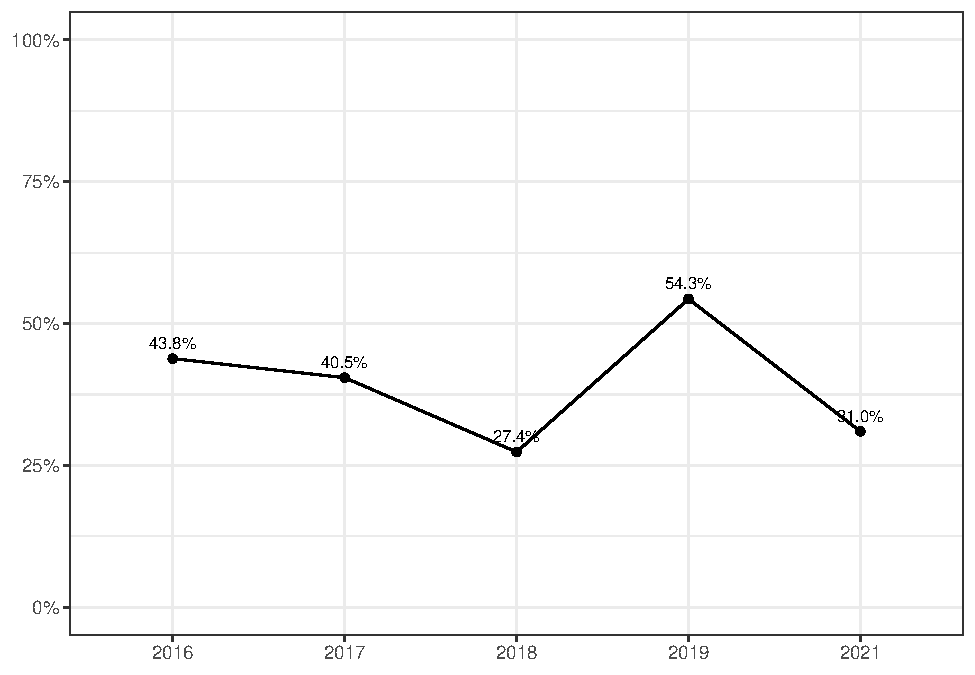
\includegraphics{reporte-elsoc_files/figure-latex/unnamed-chunk-24-1.pdf}

\hypertarget{con-cuuxe1l-de-las-siguientes-frases-estuxe1-usted-muxe1s-de-acuerdo-2021-seguxfan-posiciuxf3n-ideoluxf3gica}{%
\subsection{3.3 ¿Con cuál de las siguientes frases está usted más de acuerdo? (2021), según posición ideológica}\label{con-cuuxe1l-de-las-siguientes-frases-estuxe1-usted-muxe1s-de-acuerdo-2021-seguxfan-posiciuxf3n-ideoluxf3gica}}

\begin{Shaded}
\begin{Highlighting}[]
\NormalTok{elsoc\_long\_2016\_2021 }\SpecialCharTok{\%\textgreater{}\%}
  \FunctionTok{filter}\NormalTok{(tipo\_atricion }\SpecialCharTok{==} \DecValTok{1} \SpecialCharTok{\&} \SpecialCharTok{!}\NormalTok{c25 }\SpecialCharTok{\%in\%} \FunctionTok{c}\NormalTok{(}\SpecialCharTok{{-}}\DecValTok{888}\NormalTok{,}\SpecialCharTok{{-}}\DecValTok{999}\NormalTok{) }\SpecialCharTok{\&} 
           \SpecialCharTok{!}\NormalTok{c15 }\SpecialCharTok{\%in\%} \FunctionTok{c}\NormalTok{(}\SpecialCharTok{{-}}\DecValTok{888}\NormalTok{, }\SpecialCharTok{{-}}\DecValTok{999}\NormalTok{) }\SpecialCharTok{\&}\NormalTok{ ola }\SpecialCharTok{==} \DecValTok{5}\NormalTok{) }\SpecialCharTok{\%\textgreater{}\%}
  \FunctionTok{mutate}\NormalTok{(}\AttributeTok{pos\_id =} \FunctionTok{factor}\NormalTok{(car}\SpecialCharTok{::}\FunctionTok{recode}\NormalTok{(c15, }\AttributeTok{recodes =} \StringTok{"0:4 = 1; 5 = 2; 6:10 = 3; 11:12 = 4"}\NormalTok{),}
                     \AttributeTok{levels =} \FunctionTok{c}\NormalTok{(}\DecValTok{1}\NormalTok{, }\DecValTok{2}\NormalTok{, }\DecValTok{3}\NormalTok{, }\DecValTok{4}\NormalTok{),}
                     \AttributeTok{labels =} \FunctionTok{c}\NormalTok{(}\StringTok{\textquotesingle{}Izquierda\textquotesingle{}}\NormalTok{, }\StringTok{"Centro"}\NormalTok{, }\StringTok{"Derecha"}\NormalTok{, }\StringTok{"No se identifica"}\NormalTok{)),}
         \AttributeTok{c25 =} \FunctionTok{factor}\NormalTok{(c25, }
                      \AttributeTok{levels =} \FunctionTok{c}\NormalTok{(}\DecValTok{1}\NormalTok{, }\DecValTok{2}\NormalTok{, }\DecValTok{3}\NormalTok{, }\DecValTok{4}\NormalTok{),}
                      \AttributeTok{labels =} \FunctionTok{c}\NormalTok{(}\StringTok{\textquotesingle{}Democracia es preferible}\SpecialCharTok{\textbackslash{}n}\StringTok{a cualquier otra forma}\SpecialCharTok{\textbackslash{}n}\StringTok{de gobierno\textquotesingle{}}\NormalTok{, }
                                 \StringTok{\textquotesingle{}En algunos casos,}\SpecialCharTok{\textbackslash{}n}\StringTok{ gobierno autoritario puede}\SpecialCharTok{\textbackslash{}n}\StringTok{ ser preferible\textquotesingle{}}\NormalTok{,}
                                 \StringTok{\textquotesingle{}Da lo mismo régimen}\SpecialCharTok{\textbackslash{}n}\StringTok{democrático o autoritario\textquotesingle{}}\NormalTok{, }
                                 \StringTok{\textquotesingle{}Ninguna\textquotesingle{}}\NormalTok{))) }\SpecialCharTok{\%\textgreater{}\%}
  \FunctionTok{prop}\NormalTok{(}\AttributeTok{x =}\NormalTok{ c25, }\AttributeTok{by =}\NormalTok{ pos\_id, }\AttributeTok{na.rm =} \ConstantTok{TRUE}\NormalTok{) }\SpecialCharTok{\%\textgreater{}\%} 
\NormalTok{  sjlabelled}\SpecialCharTok{::}\FunctionTok{as\_label}\NormalTok{(pos\_id) }\SpecialCharTok{\%\textgreater{}\%} 
  \FunctionTok{ggplot}\NormalTok{(}\FunctionTok{aes}\NormalTok{(}\AttributeTok{y =}\NormalTok{ prop, }\AttributeTok{x =}\NormalTok{ pos\_id, }\AttributeTok{fill =}\NormalTok{ c25, }
             \AttributeTok{label =}\NormalTok{ scales}\SpecialCharTok{::}\FunctionTok{percent}\NormalTok{(}\FunctionTok{ifelse}\NormalTok{(prop }\SpecialCharTok{\textless{}}\NormalTok{ .}\DecValTok{01}\NormalTok{, }\ConstantTok{NA}\NormalTok{, prop), }\AttributeTok{accuracy =}\NormalTok{ .}\DecValTok{1}\NormalTok{))) }\SpecialCharTok{+} 
  \FunctionTok{theme\_bw}\NormalTok{() }\SpecialCharTok{+} 
  \FunctionTok{geom\_col}\NormalTok{(}\AttributeTok{position =} \StringTok{\textquotesingle{}Stack\textquotesingle{}}\NormalTok{) }\SpecialCharTok{+}
  \FunctionTok{scale\_y\_continuous}\NormalTok{(}\AttributeTok{labels =}\NormalTok{ scales}\SpecialCharTok{::}\NormalTok{percent) }\SpecialCharTok{+}
  \FunctionTok{ylab}\NormalTok{(}\AttributeTok{label =} \ConstantTok{NULL}\NormalTok{) }\SpecialCharTok{+}
  \FunctionTok{xlab}\NormalTok{(}\AttributeTok{label =} \ConstantTok{NULL}\NormalTok{) }\SpecialCharTok{+}
  \FunctionTok{scale\_fill\_viridis\_d}\NormalTok{(}\AttributeTok{begin =} \DecValTok{0}\NormalTok{, }\AttributeTok{end =}\NormalTok{ .}\DecValTok{95}\NormalTok{, }\AttributeTok{direction =} \SpecialCharTok{{-}}\DecValTok{1}\NormalTok{, }\AttributeTok{option =} \StringTok{\textquotesingle{}viridis\textquotesingle{}}\NormalTok{) }\SpecialCharTok{+}
  \FunctionTok{geom\_text}\NormalTok{(}\AttributeTok{position =} \FunctionTok{position\_stack}\NormalTok{(}\AttributeTok{vjust =}\NormalTok{ .}\DecValTok{5}\NormalTok{),}
            \AttributeTok{size=} \FloatTok{2.75}\NormalTok{,}
            \AttributeTok{color =} \FunctionTok{rep}\NormalTok{(}\FunctionTok{c}\NormalTok{(}\StringTok{\textquotesingle{}black\textquotesingle{}}\NormalTok{, }\StringTok{\textquotesingle{}black\textquotesingle{}}\NormalTok{, }\StringTok{\textquotesingle{}white\textquotesingle{}}\NormalTok{, }\StringTok{\textquotesingle{}white\textquotesingle{}}\NormalTok{), }\DecValTok{4}\NormalTok{)) }\SpecialCharTok{+} 
  \FunctionTok{theme}\NormalTok{(}\AttributeTok{legend.position =} \StringTok{\textquotesingle{}top\textquotesingle{}}\NormalTok{,}
        \AttributeTok{legend.title =} \FunctionTok{element\_blank}\NormalTok{())}
\end{Highlighting}
\end{Shaded}

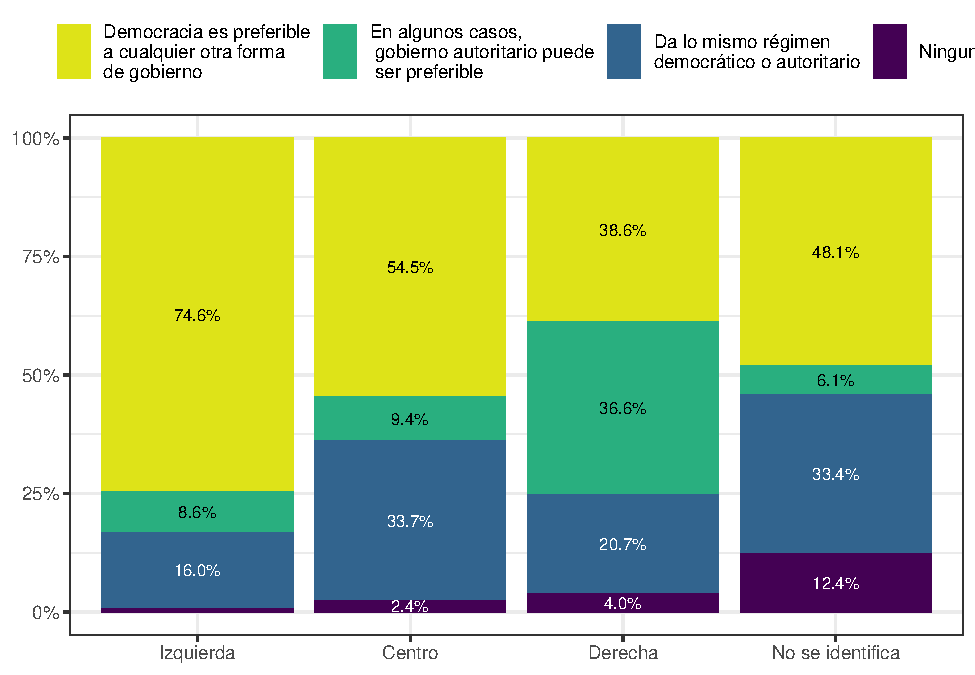
\includegraphics{reporte-elsoc_files/figure-latex/unnamed-chunk-25-1.pdf}

\hypertarget{perfiles-ideoluxf3gicos-de-los-chilenos}{%
\chapter{Perfiles Ideológicos de los Chilenos}\label{perfiles-ideoluxf3gicos-de-los-chilenos}}

\hypertarget{clases-latentes-motivaciuxf3n}{%
\section{Clases latentes: Motivación}\label{clases-latentes-motivaciuxf3n}}

\hypertarget{bateruxeda-de-preguntas}{%
\subsection{Batería de preguntas}\label{bateruxeda-de-preguntas}}

\begin{itemize}
\tightlist
\item
  Las parejas homosexuales deberían poder adoptar hijos
\item
  El aborto debe ser legal bajo cualquier circunstancia
\item
  El Estado de Chile, más que los privados, debería ser el principal proveedor de educación
\item
  Cada persona debiera asegurarse por sí mismo su futura pensión para la tercera edad
\item
  Chile debería tomar medidas más drásticas para impedir el ingreso de inmigrantes al país
\item
  La educación sexual de los niños debería ser responsabilidad exclusiva de los padres
\item
  Se deberían clausurar empresas contaminantes, incluso si esto implica un aumento en el desempleo
\item
  El gasto social debe destinarse únicamente a los más pobres y vulnerables
\end{itemize}

\hypertarget{modelo-teuxf3rico-de-perfiles-ideuxf3logicos}{%
\section{Modelo teórico de perfiles ideólogicos}\label{modelo-teuxf3rico-de-perfiles-ideuxf3logicos}}

\hypertarget{aproximaciuxf3n-empuxedrica}{%
\subsection{Aproximación Empírica}\label{aproximaciuxf3n-empuxedrica}}

\hypertarget{perfiles-ideoluxf3gicos-resultados-principales}{%
\subsection{Perfiles ideológicos: Resultados principales}\label{perfiles-ideoluxf3gicos-resultados-principales}}

\hypertarget{justificaciuxf3n-de-la-violencia}{%
\chapter{Justificación de la Violencia}\label{justificaciuxf3n-de-la-violencia}}

\hypertarget{justificaciuxf3n-de-la-violencia-para-el-control-social-a-manos-de-ciudadanos}{%
\section{Justificación de la violencia para el control social -- a manos de ciudadanos}\label{justificaciuxf3n-de-la-violencia-para-el-control-social-a-manos-de-ciudadanos}}

\begin{Shaded}
\begin{Highlighting}[]
\NormalTok{elsoc\_long\_2016\_2021 }\SpecialCharTok{\%\textgreater{}\%} 
  \FunctionTok{filter}\NormalTok{(tipo\_atricion }\SpecialCharTok{==} \DecValTok{1} \SpecialCharTok{\&}\NormalTok{ ola }\SpecialCharTok{\%in\%} \DecValTok{1}\SpecialCharTok{:}\DecValTok{4} \SpecialCharTok{\&}
           \SpecialCharTok{!}\NormalTok{f05\_01 }\SpecialCharTok{\%in\%} \FunctionTok{c}\NormalTok{(}\SpecialCharTok{{-}}\DecValTok{888}\NormalTok{, }\SpecialCharTok{{-}}\DecValTok{999}\NormalTok{) }\SpecialCharTok{\&} \SpecialCharTok{!}\NormalTok{f05\_02 }\SpecialCharTok{\%in\%} \FunctionTok{c}\NormalTok{(}\SpecialCharTok{{-}}\DecValTok{888}\NormalTok{, }\SpecialCharTok{{-}}\DecValTok{999}\NormalTok{)) }\SpecialCharTok{\%\textgreater{}\%}  
  \FunctionTok{select}\NormalTok{(f05\_01, f05\_02, ola, ponderador02, segmento\_disenno, estrato\_disenno) }\SpecialCharTok{\%\textgreater{}\%} 
  \FunctionTok{pivot\_longer}\NormalTok{(}\AttributeTok{cols =} \FunctionTok{c}\NormalTok{(f05\_01, f05\_02)) }\SpecialCharTok{\%\textgreater{}\%} 
  \FunctionTok{prop}\NormalTok{(value }\SpecialCharTok{\%in\%} \DecValTok{4}\SpecialCharTok{:}\DecValTok{5}\NormalTok{, }\AttributeTok{by =} \FunctionTok{c}\NormalTok{(ola, name), }\AttributeTok{na.rm =} \ConstantTok{TRUE}\NormalTok{) }\SpecialCharTok{\%\textgreater{}\%} 
  \FunctionTok{mutate}\NormalTok{(}\AttributeTok{name =} \FunctionTok{factor}\NormalTok{(name,}
                       \AttributeTok{levels =} \FunctionTok{c}\NormalTok{(}\StringTok{\textquotesingle{}f05\_01\textquotesingle{}}\NormalTok{, }\StringTok{\textquotesingle{}f05\_02\textquotesingle{}}\NormalTok{),}
                       \AttributeTok{labels =} \FunctionTok{c}\NormalTok{(}\StringTok{\textquotesingle{}Personas persigan y golpeen a un delincuente}\SpecialCharTok{\textbackslash{}n}\StringTok{ que acaba de cometer un asalto\textquotesingle{}}\NormalTok{,}\StringTok{\textquotesingle{}Personas amarren a un poste y desnuden a un}\SpecialCharTok{\textbackslash{}n}\StringTok{ delincuente que acaba de cometer un asalto\textquotesingle{}}\NormalTok{))) }\SpecialCharTok{\%\textgreater{}\%} 
\NormalTok{sjlabelled}\SpecialCharTok{::}\FunctionTok{as\_label}\NormalTok{(ola) }\SpecialCharTok{\%\textgreater{}\%} 
  \FunctionTok{ggplot}\NormalTok{(}\FunctionTok{aes}\NormalTok{(}\AttributeTok{y =}\NormalTok{ prop, }\AttributeTok{x =}\NormalTok{ ola, }\AttributeTok{color =}\NormalTok{ name, }\AttributeTok{group =}\NormalTok{ name,}
             \AttributeTok{label =}\NormalTok{ scales}\SpecialCharTok{::}\FunctionTok{percent}\NormalTok{(prop, }\AttributeTok{accuracy =}\NormalTok{ .}\DecValTok{1}\NormalTok{))) }\SpecialCharTok{+}
  \FunctionTok{theme\_bw}\NormalTok{() }\SpecialCharTok{+} 
  \FunctionTok{geom\_point}\NormalTok{() }\SpecialCharTok{+} 
  \FunctionTok{geom\_line}\NormalTok{() }\SpecialCharTok{+} 
  \FunctionTok{scale\_y\_continuous}\NormalTok{(}\AttributeTok{labels =}\NormalTok{ scales}\SpecialCharTok{::}\NormalTok{percent,}
                     \AttributeTok{limits =} \FunctionTok{c}\NormalTok{(}\DecValTok{0}\NormalTok{, .}\DecValTok{5}\NormalTok{)) }\SpecialCharTok{+}
  \FunctionTok{ylab}\NormalTok{(}\AttributeTok{label =} \ConstantTok{NULL}\NormalTok{) }\SpecialCharTok{+}
  \FunctionTok{xlab}\NormalTok{(}\AttributeTok{label =} \ConstantTok{NULL}\NormalTok{) }\SpecialCharTok{+}
  \FunctionTok{scale\_color\_viridis\_d}\NormalTok{(}\AttributeTok{begin =}\NormalTok{ .}\DecValTok{33}\NormalTok{, }\AttributeTok{end =}\NormalTok{ .}\DecValTok{66}\NormalTok{, }\AttributeTok{direction =} \SpecialCharTok{{-}}\DecValTok{1}\NormalTok{, }\AttributeTok{option =} \StringTok{\textquotesingle{}viridis\textquotesingle{}}\NormalTok{) }\SpecialCharTok{+} 
  \FunctionTok{geom\_text\_repel}\NormalTok{() }\SpecialCharTok{+}
  \FunctionTok{theme}\NormalTok{(}\AttributeTok{legend.position =} \StringTok{\textquotesingle{}top\textquotesingle{}}\NormalTok{,}
        \AttributeTok{legend.title =} \FunctionTok{element\_blank}\NormalTok{())}
\end{Highlighting}
\end{Shaded}

\begin{figure}
\centering
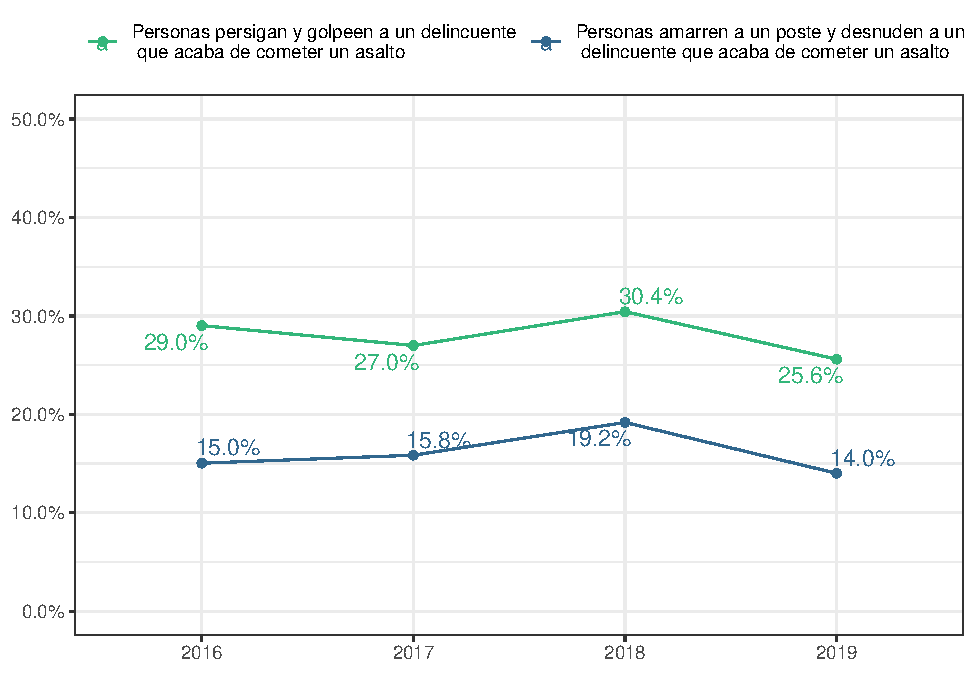
\includegraphics{reporte-elsoc_files/figure-latex/just-vio-ola-1.pdf}
\caption{\label{fig:just-vio-ola}Justificación de la violencia en relación a delincuencia, según ola de encuesta}
\end{figure}

\hypertarget{justificaciuxf3n-de-la-violencia-para-el-control-social-a-manos-de-carabineros}{%
\section{Justificación de la violencia para el control social -- a manos de carabineros}\label{justificaciuxf3n-de-la-violencia-para-el-control-social-a-manos-de-carabineros}}

\begin{Shaded}
\begin{Highlighting}[]
\NormalTok{elsoc\_long\_2016\_2021 }\SpecialCharTok{\%\textgreater{}\%} 
  \FunctionTok{filter}\NormalTok{(tipo\_atricion }\SpecialCharTok{==} \DecValTok{1} \SpecialCharTok{\&}\NormalTok{ muestra }\SpecialCharTok{==} \DecValTok{1} \SpecialCharTok{\&} 
           \SpecialCharTok{!}\NormalTok{f05\_03 }\SpecialCharTok{\%in\%} \FunctionTok{c}\NormalTok{(}\SpecialCharTok{{-}}\DecValTok{888}\NormalTok{, }\SpecialCharTok{{-}}\DecValTok{999}\NormalTok{) }\SpecialCharTok{\&} \SpecialCharTok{!}\NormalTok{f05\_04 }\SpecialCharTok{\%in\%} \FunctionTok{c}\NormalTok{(}\SpecialCharTok{{-}}\DecValTok{888}\NormalTok{, }\SpecialCharTok{{-}}\DecValTok{999}\NormalTok{) }\SpecialCharTok{\&} \SpecialCharTok{!}\NormalTok{f05\_07 }\SpecialCharTok{\%in\%} \FunctionTok{c}\NormalTok{(}\SpecialCharTok{{-}}\DecValTok{888}\NormalTok{, }\SpecialCharTok{{-}}\DecValTok{999}\NormalTok{)) }\SpecialCharTok{\%\textgreater{}\%}  
  \FunctionTok{select}\NormalTok{(f05\_03, f05\_04, f05\_07, ola, ponderador02, segmento\_disenno, estrato\_disenno) }\SpecialCharTok{\%\textgreater{}\%} 
  \FunctionTok{pivot\_longer}\NormalTok{(}\AttributeTok{cols =} \FunctionTok{c}\NormalTok{(f05\_03, f05\_04, f05\_07)) }\SpecialCharTok{\%\textgreater{}\%} 
  \FunctionTok{prop}\NormalTok{(value }\SpecialCharTok{\%in\%} \DecValTok{4}\SpecialCharTok{:}\DecValTok{5}\NormalTok{, }\AttributeTok{by =} \FunctionTok{c}\NormalTok{(ola, name), }\AttributeTok{na.rm =} \ConstantTok{TRUE}\NormalTok{) }\SpecialCharTok{\%\textgreater{}\%} 
  \FunctionTok{mutate}\NormalTok{(}\AttributeTok{name =} \FunctionTok{factor}\NormalTok{(name,}
                       \AttributeTok{levels =} \FunctionTok{c}\NormalTok{(}\StringTok{\textquotesingle{}f05\_03\textquotesingle{}}\NormalTok{, }\StringTok{\textquotesingle{}f05\_04\textquotesingle{}}\NormalTok{, }\StringTok{\textquotesingle{}f05\_07\textquotesingle{}}\NormalTok{),}
                       \AttributeTok{labels =} \FunctionTok{c}\NormalTok{(}\StringTok{\textquotesingle{}Carabineros use la fuerza para}\SpecialCharTok{\textbackslash{}n}\StringTok{ reprimir manifestación pacífica\textquotesingle{}}\NormalTok{,}
                                  \StringTok{\textquotesingle{}Carabineros desaloje a la fuerza}\SpecialCharTok{\textbackslash{}n}\StringTok{a estudiantes de liceo en toma\textquotesingle{}}\NormalTok{,}
                                  \StringTok{\textquotesingle{}Estudiantes tiren piedras a Carabi{-}}\SpecialCharTok{\textbackslash{}n}\StringTok{neros en marcha por la educación\textquotesingle{}}\NormalTok{))) }\SpecialCharTok{\%\textgreater{}\%} 
\NormalTok{sjlabelled}\SpecialCharTok{::}\FunctionTok{as\_label}\NormalTok{(ola) }\SpecialCharTok{\%\textgreater{}\%} 
  \FunctionTok{ggplot}\NormalTok{(}\FunctionTok{aes}\NormalTok{(}\AttributeTok{y =}\NormalTok{ prop, }\AttributeTok{x =}\NormalTok{ ola, }\AttributeTok{color =}\NormalTok{ name, }\AttributeTok{group =}\NormalTok{ name,}
             \AttributeTok{label =}\NormalTok{ scales}\SpecialCharTok{::}\FunctionTok{percent}\NormalTok{(prop, }\AttributeTok{accuracy =}\NormalTok{ .}\DecValTok{1}\NormalTok{))) }\SpecialCharTok{+}
  \FunctionTok{theme\_bw}\NormalTok{() }\SpecialCharTok{+} 
  \FunctionTok{geom\_point}\NormalTok{() }\SpecialCharTok{+} 
  \FunctionTok{geom\_line}\NormalTok{() }\SpecialCharTok{+}
  \FunctionTok{scale\_y\_continuous}\NormalTok{(}\AttributeTok{labels =}\NormalTok{ scales}\SpecialCharTok{::}\NormalTok{percent,}
                     \AttributeTok{limits =} \FunctionTok{c}\NormalTok{(}\DecValTok{0}\NormalTok{, .}\DecValTok{5}\NormalTok{)) }\SpecialCharTok{+}
  \FunctionTok{ylab}\NormalTok{(}\AttributeTok{label =} \ConstantTok{NULL}\NormalTok{) }\SpecialCharTok{+}
  \FunctionTok{xlab}\NormalTok{(}\AttributeTok{label =} \ConstantTok{NULL}\NormalTok{) }\SpecialCharTok{+}
  \FunctionTok{scale\_color\_viridis\_d}\NormalTok{(}\AttributeTok{begin =} \DecValTok{0}\NormalTok{, }\AttributeTok{end =}\NormalTok{ .}\DecValTok{75}\NormalTok{, }\AttributeTok{option =} \StringTok{\textquotesingle{}viridis\textquotesingle{}}\NormalTok{) }\SpecialCharTok{+} 
\NormalTok{  ggrepel}\SpecialCharTok{::}\FunctionTok{geom\_text\_repel}\NormalTok{() }\SpecialCharTok{+}
  \FunctionTok{theme}\NormalTok{(}\AttributeTok{legend.position =} \StringTok{\textquotesingle{}top\textquotesingle{}}\NormalTok{,}
        \AttributeTok{legend.title =} \FunctionTok{element\_blank}\NormalTok{())}
\end{Highlighting}
\end{Shaded}

\begin{figure}

{\centering 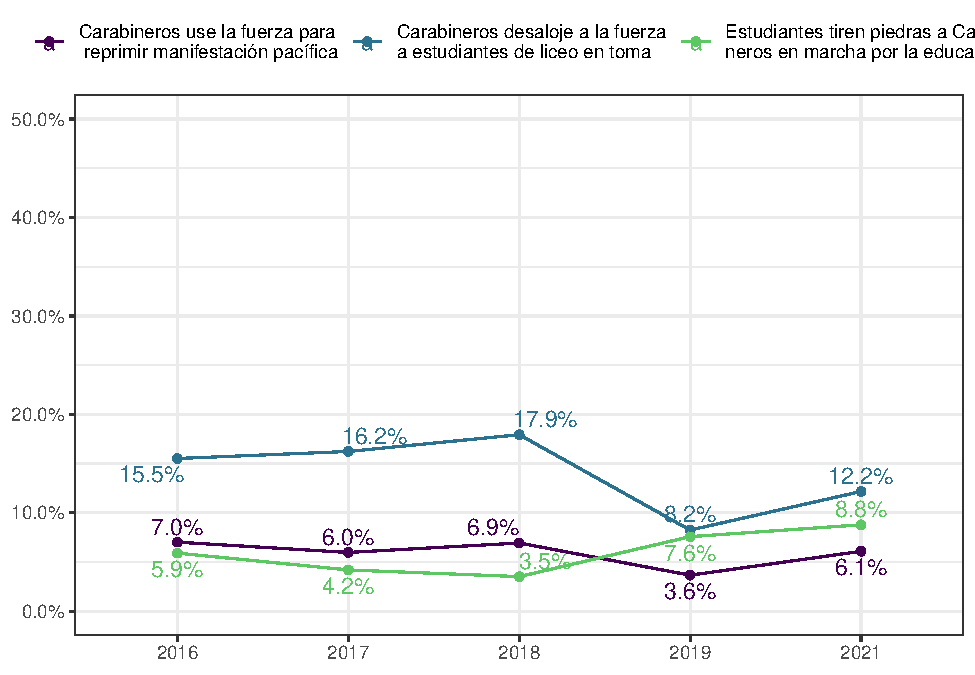
\includegraphics{reporte-elsoc_files/figure-latex/just-carab-ola-1} 

}

\caption{Justificación de la violencia en relación al actuar de Carabineros, según ola}\label{fig:just-carab-ola}
\end{figure}

\hypertarget{cambio-constitucional}{%
\chapter{Cambio Constitucional}\label{cambio-constitucional}}

\begin{Shaded}
\begin{Highlighting}[]
\NormalTok{datos.g11}\FloatTok{.1} \OtherTok{\textless{}{-}}\NormalTok{ elsoc\_long\_2016\_2021 }\SpecialCharTok{\%\textgreater{}\%} 
\NormalTok{  dplyr}\SpecialCharTok{::}\FunctionTok{filter}\NormalTok{(ola }\SpecialCharTok{==} \DecValTok{5} \SpecialCharTok{\&}\NormalTok{ tipo\_atricion }\SpecialCharTok{==} \DecValTok{1} \SpecialCharTok{\&} \SpecialCharTok{!}\NormalTok{c43 }\SpecialCharTok{\%in\%} \FunctionTok{c}\NormalTok{(}\DecValTok{3}\NormalTok{, }\SpecialCharTok{{-}}\DecValTok{888}\NormalTok{, }\SpecialCharTok{{-}}\DecValTok{999}\NormalTok{)) }\SpecialCharTok{\%\textgreater{}\%} 
  \FunctionTok{mutate}\NormalTok{(}\AttributeTok{edadt =} \FunctionTok{factor}\NormalTok{(car}\SpecialCharTok{::}\FunctionTok{recode}\NormalTok{(m0\_edad, }\StringTok{"18:29 = 1; 30:49 = 2; 50:64 = 3; 65:150 = 4"}\NormalTok{),}
                           \AttributeTok{labels =} \FunctionTok{c}\NormalTok{(}\StringTok{\textquotesingle{}18{-}29\textquotesingle{}}\NormalTok{, }\StringTok{\textquotesingle{}30{-}49\textquotesingle{}}\NormalTok{, }\StringTok{\textquotesingle{}50{-}64\textquotesingle{}}\NormalTok{, }\StringTok{\textquotesingle{}65 o más\textquotesingle{}}\NormalTok{))) }\SpecialCharTok{\%\textgreater{}\%}
  \FunctionTok{prop}\NormalTok{(c43, }\AttributeTok{by =}\NormalTok{ edadt, }\AttributeTok{na.rm =} \ConstantTok{TRUE}\NormalTok{) }\SpecialCharTok{\%\textgreater{}\%} 
\NormalTok{  sjlabelled}\SpecialCharTok{::}\FunctionTok{as\_label}\NormalTok{(c43, edadt)}
  
\NormalTok{g11}\FloatTok{.1} \OtherTok{\textless{}{-}}\NormalTok{ datos.g11}\FloatTok{.1} \SpecialCharTok{\%\textgreater{}\%} 
  \FunctionTok{ggplot}\NormalTok{(}\FunctionTok{aes}\NormalTok{(}\AttributeTok{y =}\NormalTok{ prop, }\AttributeTok{x =}\NormalTok{ edadt, }\AttributeTok{fill =}\NormalTok{ c43, }
             \AttributeTok{label =}\NormalTok{ scales}\SpecialCharTok{::}\FunctionTok{percent}\NormalTok{(prop, }\AttributeTok{accuracy =}\NormalTok{ .}\DecValTok{1}\NormalTok{))) }\SpecialCharTok{+}
  \FunctionTok{theme\_bw}\NormalTok{() }\SpecialCharTok{+} 
  \FunctionTok{geom\_col}\NormalTok{(}\AttributeTok{position =} \StringTok{\textquotesingle{}dodge2\textquotesingle{}}\NormalTok{) }\SpecialCharTok{+}
  \FunctionTok{scale\_y\_continuous}\NormalTok{(}\AttributeTok{labels =}\NormalTok{ scales}\SpecialCharTok{::}\NormalTok{percent,}
                     \AttributeTok{limits =} \FunctionTok{c}\NormalTok{(}\DecValTok{0}\NormalTok{, }\DecValTok{1}\NormalTok{)) }\SpecialCharTok{+}
  \FunctionTok{ylab}\NormalTok{(}\AttributeTok{label =} \ConstantTok{NULL}\NormalTok{) }\SpecialCharTok{+}
  \FunctionTok{xlab}\NormalTok{(}\AttributeTok{label =} \ConstantTok{NULL}\NormalTok{) }\SpecialCharTok{+}
  \FunctionTok{scale\_fill\_viridis\_d}\NormalTok{(}\AttributeTok{begin =} \DecValTok{0}\NormalTok{, }\AttributeTok{end =}\NormalTok{ .}\DecValTok{85}\NormalTok{, }\AttributeTok{direction =} \SpecialCharTok{{-}}\DecValTok{1}\NormalTok{, }\AttributeTok{option =} \StringTok{\textquotesingle{}viridis\textquotesingle{}}\NormalTok{) }\SpecialCharTok{+}
  \FunctionTok{geom\_text}\NormalTok{(}\AttributeTok{vjust =} \SpecialCharTok{{-}}\FloatTok{0.8}\NormalTok{,}
            \AttributeTok{position =} \FunctionTok{position\_dodge}\NormalTok{(}\AttributeTok{width =}\NormalTok{ .}\DecValTok{9}\NormalTok{),}
            \AttributeTok{size=} \FloatTok{2.75}\NormalTok{)  }\SpecialCharTok{+} 
  \FunctionTok{theme}\NormalTok{(}\AttributeTok{legend.position =} \StringTok{\textquotesingle{}top\textquotesingle{}}\NormalTok{,}
        \AttributeTok{legend.title =} \FunctionTok{element\_blank}\NormalTok{()) }

\NormalTok{g11}\FloatTok{.1}
\end{Highlighting}
\end{Shaded}

\begin{figure}

{\centering 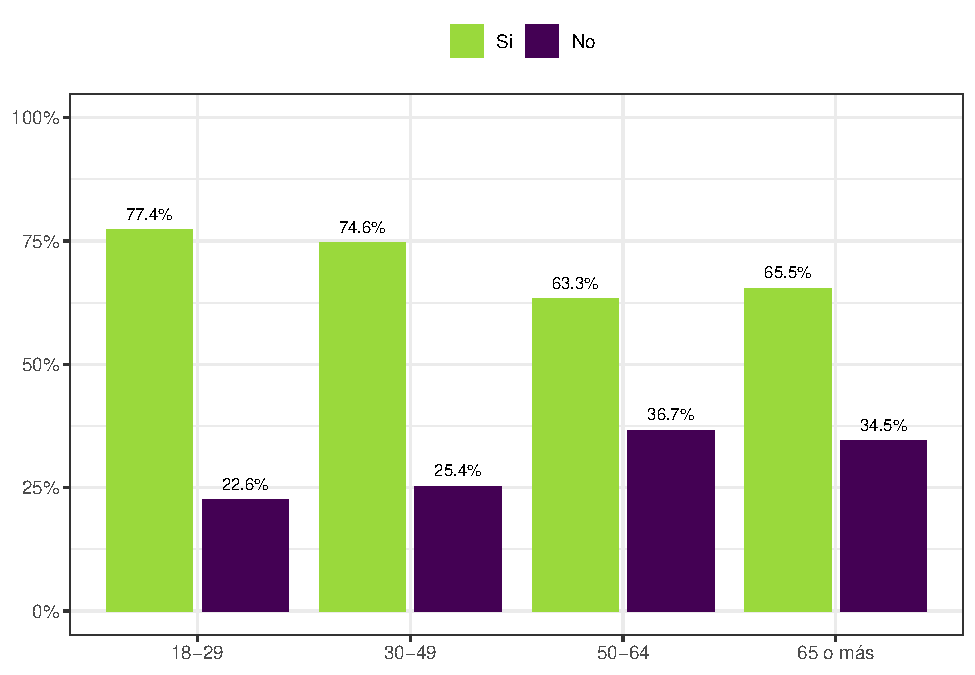
\includegraphics{reporte-elsoc_files/figure-latex/particip-edad-1} 

}

\caption{Participación en Plebiscito Nueva Constitucion}\label{fig:particip-edad}
\end{figure}

\begin{Shaded}
\begin{Highlighting}[]
\NormalTok{datos.g11}\FloatTok{.2} \OtherTok{\textless{}{-}}\NormalTok{ elsoc\_long\_2016\_2021 }\SpecialCharTok{\%\textgreater{}\%} 
\NormalTok{  dplyr}\SpecialCharTok{::}\FunctionTok{filter}\NormalTok{(ola }\SpecialCharTok{==} \DecValTok{5} \SpecialCharTok{\&}\NormalTok{ tipo\_atricion }\SpecialCharTok{==} \DecValTok{1} \SpecialCharTok{\&} \SpecialCharTok{!}\NormalTok{c44 }\SpecialCharTok{\%in\%} \FunctionTok{c}\NormalTok{(}\DecValTok{3}\NormalTok{, }\DecValTok{4}\NormalTok{, }\SpecialCharTok{{-}}\DecValTok{888}\NormalTok{, }\SpecialCharTok{{-}}\DecValTok{999}\NormalTok{)}\SpecialCharTok{\&} \SpecialCharTok{!}\FunctionTok{is.na}\NormalTok{(c44)) }\SpecialCharTok{\%\textgreater{}\%} 
  \FunctionTok{prop}\NormalTok{(c44, }\AttributeTok{na.rm =} \ConstantTok{TRUE}\NormalTok{, }\AttributeTok{vartype =} \ConstantTok{NULL}\NormalTok{) }\SpecialCharTok{\%\textgreater{}\%} 
\NormalTok{  sjlabelled}\SpecialCharTok{::}\FunctionTok{as\_label}\NormalTok{(c44) }\SpecialCharTok{\%\textgreater{}\%} 
  \FunctionTok{mutate}\NormalTok{(}\AttributeTok{datos =} \StringTok{\textquotesingle{}Datos ELSOC\textquotesingle{}}\NormalTok{) }\SpecialCharTok{\%\textgreater{}\%}
  \FunctionTok{add\_row}\NormalTok{(}\AttributeTok{c44 =} \FunctionTok{c}\NormalTok{(}\StringTok{\textquotesingle{}Apruebo\textquotesingle{}}\NormalTok{, }\StringTok{\textquotesingle{}Rechazo\textquotesingle{}}\NormalTok{), }\AttributeTok{prop =} \FunctionTok{c}\NormalTok{(.}\DecValTok{7828}\NormalTok{, .}\DecValTok{2172}\NormalTok{), }\AttributeTok{datos =} \FunctionTok{c}\NormalTok{(}\StringTok{\textquotesingle{}Datos servel\textquotesingle{}}\NormalTok{, }\StringTok{\textquotesingle{}Datos servel\textquotesingle{}}\NormalTok{))}

\NormalTok{g11}\FloatTok{.2} \OtherTok{\textless{}{-}}\NormalTok{ datos.g11}\FloatTok{.2} \SpecialCharTok{\%\textgreater{}\%} 
  \FunctionTok{ggplot}\NormalTok{(}\FunctionTok{aes}\NormalTok{(}\AttributeTok{y =}\NormalTok{ prop, }\AttributeTok{x =}\NormalTok{ datos, }\AttributeTok{fill =}\NormalTok{ c44, }
             \AttributeTok{label =}\NormalTok{ scales}\SpecialCharTok{::}\FunctionTok{percent}\NormalTok{(prop, }\AttributeTok{accuracy =}\NormalTok{ .}\DecValTok{1}\NormalTok{))) }\SpecialCharTok{+}
  \FunctionTok{theme\_bw}\NormalTok{() }\SpecialCharTok{+} 
  \FunctionTok{geom\_col}\NormalTok{(}\AttributeTok{position =} \StringTok{\textquotesingle{}dodge2\textquotesingle{}}\NormalTok{) }\SpecialCharTok{+}
  \FunctionTok{scale\_y\_continuous}\NormalTok{(}\AttributeTok{labels =}\NormalTok{ scales}\SpecialCharTok{::}\NormalTok{percent,}
                     \AttributeTok{limits =} \FunctionTok{c}\NormalTok{(}\DecValTok{0}\NormalTok{, }\DecValTok{1}\NormalTok{)) }\SpecialCharTok{+}
  \FunctionTok{ylab}\NormalTok{(}\AttributeTok{label =} \ConstantTok{NULL}\NormalTok{) }\SpecialCharTok{+}
  \FunctionTok{xlab}\NormalTok{(}\AttributeTok{label =} \ConstantTok{NULL}\NormalTok{) }\SpecialCharTok{+}
  \FunctionTok{scale\_fill\_viridis\_d}\NormalTok{(}\AttributeTok{begin =} \DecValTok{0}\NormalTok{, }\AttributeTok{end =}\NormalTok{ .}\DecValTok{85}\NormalTok{, }\AttributeTok{direction =} \SpecialCharTok{{-}}\DecValTok{1}\NormalTok{, }\AttributeTok{option =} \StringTok{\textquotesingle{}viridis\textquotesingle{}}\NormalTok{) }\SpecialCharTok{+}
  \FunctionTok{geom\_text}\NormalTok{(}\AttributeTok{vjust =} \SpecialCharTok{{-}}\FloatTok{0.8}\NormalTok{,}
            \AttributeTok{position =} \FunctionTok{position\_dodge}\NormalTok{(}\AttributeTok{width =}\NormalTok{ .}\DecValTok{9}\NormalTok{),}
            \AttributeTok{size=} \FloatTok{2.75}\NormalTok{)  }\SpecialCharTok{+} 
  \FunctionTok{theme}\NormalTok{(}\AttributeTok{legend.position =} \StringTok{\textquotesingle{}top\textquotesingle{}}\NormalTok{,}
        \AttributeTok{legend.title =} \FunctionTok{element\_blank}\NormalTok{())}

\NormalTok{g11}\FloatTok{.2}
\end{Highlighting}
\end{Shaded}

\begin{figure}

{\centering 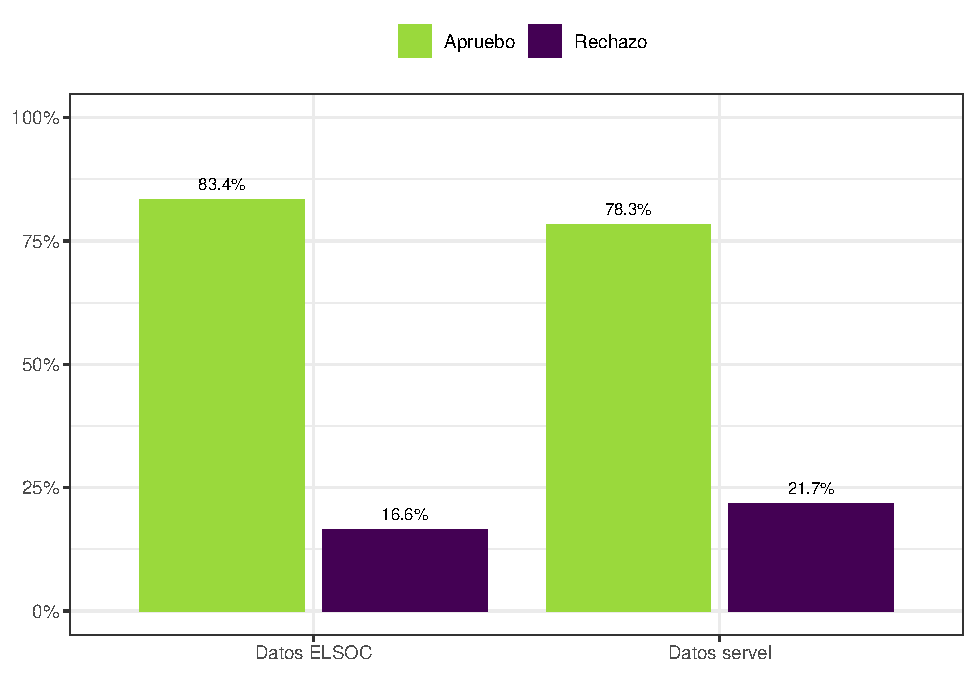
\includegraphics{reporte-elsoc_files/figure-latex/servel-apruebo-1} 

}

\caption{Voto retrospectivo Plebiscito Nueva Constitucion}\label{fig:servel-apruebo}
\end{figure}

\begin{Shaded}
\begin{Highlighting}[]
\NormalTok{datos.g11}\FloatTok{.3} \OtherTok{\textless{}{-}}\NormalTok{ elsoc\_long\_2016\_2021 }\SpecialCharTok{\%\textgreater{}\%} 
\NormalTok{  dplyr}\SpecialCharTok{::}\FunctionTok{filter}\NormalTok{(ola }\SpecialCharTok{==} \DecValTok{5} \SpecialCharTok{\&}\NormalTok{ tipo\_atricion }\SpecialCharTok{==} \DecValTok{1} \SpecialCharTok{\&} \SpecialCharTok{!}\NormalTok{c45 }\SpecialCharTok{\%in\%} \FunctionTok{c}\NormalTok{(}\DecValTok{3}\NormalTok{, }\DecValTok{4}\NormalTok{, }\SpecialCharTok{{-}}\DecValTok{888}\NormalTok{, }\SpecialCharTok{{-}}\DecValTok{999}\NormalTok{) }\SpecialCharTok{\&} \SpecialCharTok{!}\FunctionTok{is.na}\NormalTok{(c45)) }\SpecialCharTok{\%\textgreater{}\%} 
  \FunctionTok{prop}\NormalTok{(c45, }\AttributeTok{na.rm =} \ConstantTok{TRUE}\NormalTok{, }\AttributeTok{vartype =} \ConstantTok{NULL}\NormalTok{) }\SpecialCharTok{\%\textgreater{}\%} 
\NormalTok{  sjlabelled}\SpecialCharTok{::}\FunctionTok{as\_label}\NormalTok{(c45) }\SpecialCharTok{\%\textgreater{}\%} 
  \FunctionTok{mutate}\NormalTok{(}\AttributeTok{datos =} \StringTok{\textquotesingle{}Datos ELSOC\textquotesingle{}}\NormalTok{) }\SpecialCharTok{\%\textgreater{}\%}
  \FunctionTok{add\_row}\NormalTok{(}\AttributeTok{c45 =} \FunctionTok{c}\NormalTok{(}\StringTok{\textquotesingle{}Convencion Mixta\textquotesingle{}}\NormalTok{, }\StringTok{\textquotesingle{}Convencion Constitucional\textquotesingle{}}\NormalTok{), }\AttributeTok{prop =} \FunctionTok{c}\NormalTok{(.}\DecValTok{2101}\NormalTok{, .}\DecValTok{7899}\NormalTok{), }\AttributeTok{datos =} \FunctionTok{c}\NormalTok{(}\StringTok{\textquotesingle{}Datos servel\textquotesingle{}}\NormalTok{, }\StringTok{\textquotesingle{}Datos servel\textquotesingle{}}\NormalTok{))}

\NormalTok{g11}\FloatTok{.3} \OtherTok{\textless{}{-}}\NormalTok{ datos.g11}\FloatTok{.3} \SpecialCharTok{\%\textgreater{}\%} 
  \FunctionTok{ggplot}\NormalTok{(}\FunctionTok{aes}\NormalTok{(}\AttributeTok{y =}\NormalTok{ prop, }\AttributeTok{x =}\NormalTok{ datos, }\AttributeTok{fill =}\NormalTok{ c45, }
             \AttributeTok{label =} \FunctionTok{as.character}\NormalTok{(scales}\SpecialCharTok{::}\FunctionTok{percent}\NormalTok{(prop, }\AttributeTok{accuracy =}\NormalTok{ .}\DecValTok{1}\NormalTok{)))) }\SpecialCharTok{+}
  \FunctionTok{theme\_bw}\NormalTok{() }\SpecialCharTok{+} 
  \FunctionTok{geom\_col}\NormalTok{(}\AttributeTok{position =} \StringTok{\textquotesingle{}dodge2\textquotesingle{}}\NormalTok{) }\SpecialCharTok{+}
  \FunctionTok{scale\_y\_continuous}\NormalTok{(}\AttributeTok{labels =}\NormalTok{ scales}\SpecialCharTok{::}\NormalTok{percent,}
                     \AttributeTok{limits =} \FunctionTok{c}\NormalTok{(}\DecValTok{0}\NormalTok{, }\DecValTok{1}\NormalTok{)) }\SpecialCharTok{+}
  \FunctionTok{ylab}\NormalTok{(}\AttributeTok{label =} \ConstantTok{NULL}\NormalTok{) }\SpecialCharTok{+}
  \FunctionTok{xlab}\NormalTok{(}\AttributeTok{label =} \ConstantTok{NULL}\NormalTok{) }\SpecialCharTok{+}
  \FunctionTok{scale\_fill\_viridis\_d}\NormalTok{(}\AttributeTok{begin =} \DecValTok{0}\NormalTok{, }\AttributeTok{end =}\NormalTok{ .}\DecValTok{85}\NormalTok{, }\AttributeTok{direction =} \SpecialCharTok{{-}}\DecValTok{1}\NormalTok{, }\AttributeTok{option =} \StringTok{\textquotesingle{}viridis\textquotesingle{}}\NormalTok{) }\SpecialCharTok{+}
  \FunctionTok{geom\_text}\NormalTok{(}\AttributeTok{vjust =} \SpecialCharTok{{-}}\FloatTok{0.8}\NormalTok{,}
            \AttributeTok{position =} \FunctionTok{position\_dodge}\NormalTok{(}\AttributeTok{width =}\NormalTok{ .}\DecValTok{9}\NormalTok{),}
            \AttributeTok{size=} \FloatTok{2.75}\NormalTok{)  }\SpecialCharTok{+} 
  \FunctionTok{theme}\NormalTok{(}\AttributeTok{legend.position =} \StringTok{\textquotesingle{}top\textquotesingle{}}\NormalTok{,}
        \AttributeTok{legend.title =} \FunctionTok{element\_blank}\NormalTok{())}

\NormalTok{g11}\FloatTok{.3}
\end{Highlighting}
\end{Shaded}

\begin{figure}

{\centering 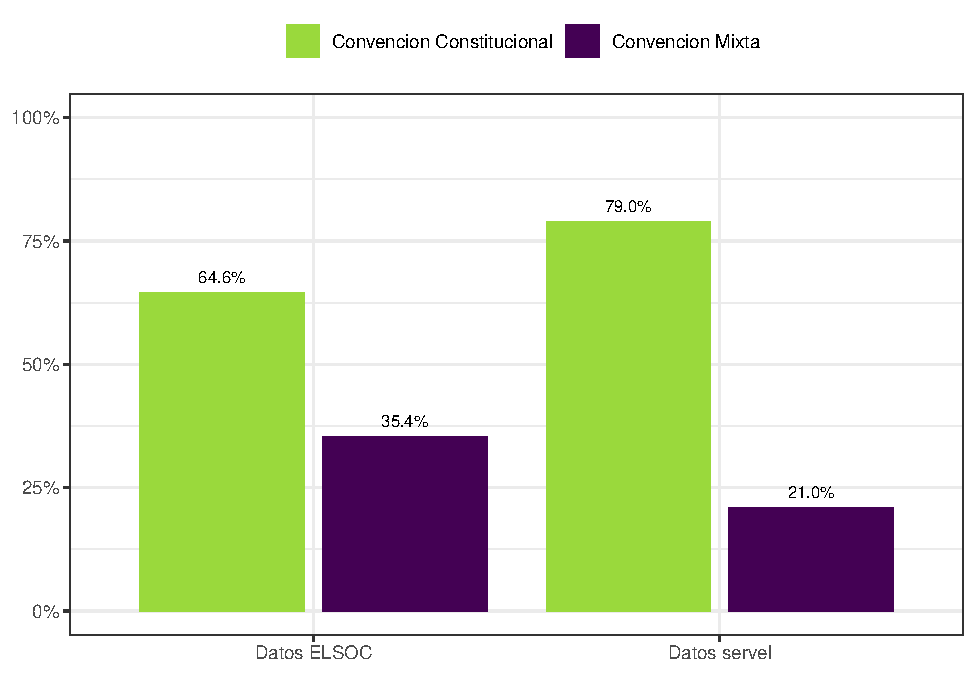
\includegraphics{reporte-elsoc_files/figure-latex/servel-cc-1} 

}

\caption{Voto Retrospectivo Plebiscito Nueva Constitucion}\label{fig:servel-cc}
\end{figure}

\begin{Shaded}
\begin{Highlighting}[]
\NormalTok{datos.g11}\FloatTok{.4} \OtherTok{\textless{}{-}}\NormalTok{ elsoc\_long\_2016\_2021 }\SpecialCharTok{\%\textgreater{}\%} 
  \FunctionTok{mutate}\NormalTok{(}\AttributeTok{c11 =}\NormalTok{ car}\SpecialCharTok{::}\FunctionTok{recode}\NormalTok{(c11, }\StringTok{\textquotesingle{}1=2;2=1\textquotesingle{}}\NormalTok{), }\CommentTok{\# en c11 1 = no participa, a diferencia de c43}
         \AttributeTok{particip\_electoral =} \FunctionTok{ifelse}\NormalTok{(ola }\SpecialCharTok{==} \DecValTok{5}\NormalTok{, c43, c11),}
         \AttributeTok{pos\_id =} \FunctionTok{factor}\NormalTok{(car}\SpecialCharTok{::}\FunctionTok{recode}\NormalTok{(c15, }\AttributeTok{recodes =} \StringTok{"0:4 = 1; 5 = 2; 6:10 = 3; 11:12 = 4"}\NormalTok{),}
                         \AttributeTok{levels =} \FunctionTok{c}\NormalTok{(}\DecValTok{1}\NormalTok{, }\DecValTok{2}\NormalTok{, }\DecValTok{3}\NormalTok{, }\DecValTok{4}\NormalTok{),}
                         \AttributeTok{labels =} \FunctionTok{c}\NormalTok{(}\StringTok{\textquotesingle{}Izquierda\textquotesingle{}}\NormalTok{, }\StringTok{"Centro"}\NormalTok{, }\StringTok{"Derecha"}\NormalTok{, }\StringTok{"No se identifica"}\NormalTok{))) }\SpecialCharTok{\%\textgreater{}\%}
  \FunctionTok{filter}\NormalTok{(tipo\_atricion }\SpecialCharTok{==} \DecValTok{1} \SpecialCharTok{\&} \SpecialCharTok{!}\NormalTok{particip\_electoral }\SpecialCharTok{\%in\%} \FunctionTok{c}\NormalTok{(}\DecValTok{3}\NormalTok{, }\SpecialCharTok{{-}}\DecValTok{888}\NormalTok{, }\SpecialCharTok{{-}}\DecValTok{999}\NormalTok{) }\SpecialCharTok{\&} 
\NormalTok{           ola }\SpecialCharTok{\%in\%} \FunctionTok{c}\NormalTok{(}\DecValTok{1}\NormalTok{,}\DecValTok{3}\NormalTok{,}\DecValTok{5}\NormalTok{) }\SpecialCharTok{\&} \SpecialCharTok{!}\FunctionTok{is.na}\NormalTok{(pos\_id)) }\SpecialCharTok{\%\textgreater{}\%} 
  \FunctionTok{prop}\NormalTok{(particip\_electoral }\SpecialCharTok{==} \DecValTok{1}\NormalTok{, }\AttributeTok{by =} \FunctionTok{c}\NormalTok{(ola, pos\_id), }\AttributeTok{na.rm =} \ConstantTok{TRUE}\NormalTok{) }\SpecialCharTok{\%\textgreater{}\%}
\NormalTok{  sjlabelled}\SpecialCharTok{::}\FunctionTok{as\_label}\NormalTok{(pos\_id) }\SpecialCharTok{\%\textgreater{}\%} 
  \FunctionTok{mutate}\NormalTok{(}\AttributeTok{ola =} \FunctionTok{factor}\NormalTok{(ola, }\AttributeTok{levels =} \FunctionTok{c}\NormalTok{(}\DecValTok{1}\NormalTok{,}\DecValTok{3}\NormalTok{,}\DecValTok{5}\NormalTok{), }\AttributeTok{labels =} \FunctionTok{c}\NormalTok{(}\StringTok{\textquotesingle{}Elecciones Presidenciales}\SpecialCharTok{\textbackslash{}n}\StringTok{de 2013\textquotesingle{}}\NormalTok{, }\StringTok{\textquotesingle{}Elecciones Presidenciales}\SpecialCharTok{\textbackslash{}n}\StringTok{de 2017\textquotesingle{}}\NormalTok{, }\StringTok{\textquotesingle{}Plebiscito cambio}\SpecialCharTok{\textbackslash{}n}\StringTok{constitucional\textquotesingle{}}\NormalTok{)))}


\NormalTok{g11}\FloatTok{.4} \OtherTok{\textless{}{-}}\NormalTok{ datos.g11}\FloatTok{.4} \SpecialCharTok{\%\textgreater{}\%} 
  \FunctionTok{ggplot}\NormalTok{(}\FunctionTok{aes}\NormalTok{(}\AttributeTok{y =}\NormalTok{ prop, }\AttributeTok{x =}\NormalTok{ ola, }\AttributeTok{color =}\NormalTok{ pos\_id, }\AttributeTok{group =}\NormalTok{ pos\_id,}
              \AttributeTok{label =}\NormalTok{ scales}\SpecialCharTok{::}\FunctionTok{percent}\NormalTok{(prop, }\AttributeTok{accuracy =}\NormalTok{ .}\DecValTok{1}\NormalTok{))) }\SpecialCharTok{+}
  \FunctionTok{theme\_bw}\NormalTok{() }\SpecialCharTok{+}   
  \FunctionTok{geom\_line}\NormalTok{(}\AttributeTok{size =} \DecValTok{1}\NormalTok{) }\SpecialCharTok{+}
  \FunctionTok{geom\_point}\NormalTok{(}\AttributeTok{size =} \FloatTok{1.8}\NormalTok{) }\SpecialCharTok{+}
  \FunctionTok{scale\_y\_continuous}\NormalTok{(}\AttributeTok{labels =}\NormalTok{ scales}\SpecialCharTok{::}\NormalTok{percent,}
                     \AttributeTok{limits =} \FunctionTok{c}\NormalTok{(}\DecValTok{0}\NormalTok{,}\DecValTok{1}\NormalTok{)) }\SpecialCharTok{+}
  \FunctionTok{ylab}\NormalTok{(}\AttributeTok{label =} \ConstantTok{NULL}\NormalTok{) }\SpecialCharTok{+}
  \FunctionTok{xlab}\NormalTok{(}\AttributeTok{label =} \ConstantTok{NULL}\NormalTok{) }\SpecialCharTok{+}
  \FunctionTok{scale\_color\_viridis\_d}\NormalTok{(}\AttributeTok{begin =} \FloatTok{0.22}\NormalTok{, }\AttributeTok{end =}\NormalTok{ .}\DecValTok{66}\NormalTok{, }\AttributeTok{direction =} \DecValTok{1}\NormalTok{, }\AttributeTok{option =} \StringTok{\textquotesingle{}viridis\textquotesingle{}}\NormalTok{) }\SpecialCharTok{+}
\NormalTok{  ggrepel}\SpecialCharTok{::}\FunctionTok{geom\_text\_repel}\NormalTok{(}\AttributeTok{size=} \FloatTok{2.25}\NormalTok{) }\SpecialCharTok{+} 
  \FunctionTok{theme}\NormalTok{(}\AttributeTok{legend.position =} \StringTok{\textquotesingle{}top\textquotesingle{}}\NormalTok{,}
        \AttributeTok{legend.title =} \FunctionTok{element\_blank}\NormalTok{())}

\NormalTok{g11}\FloatTok{.4}
\end{Highlighting}
\end{Shaded}

\begin{figure}

{\centering 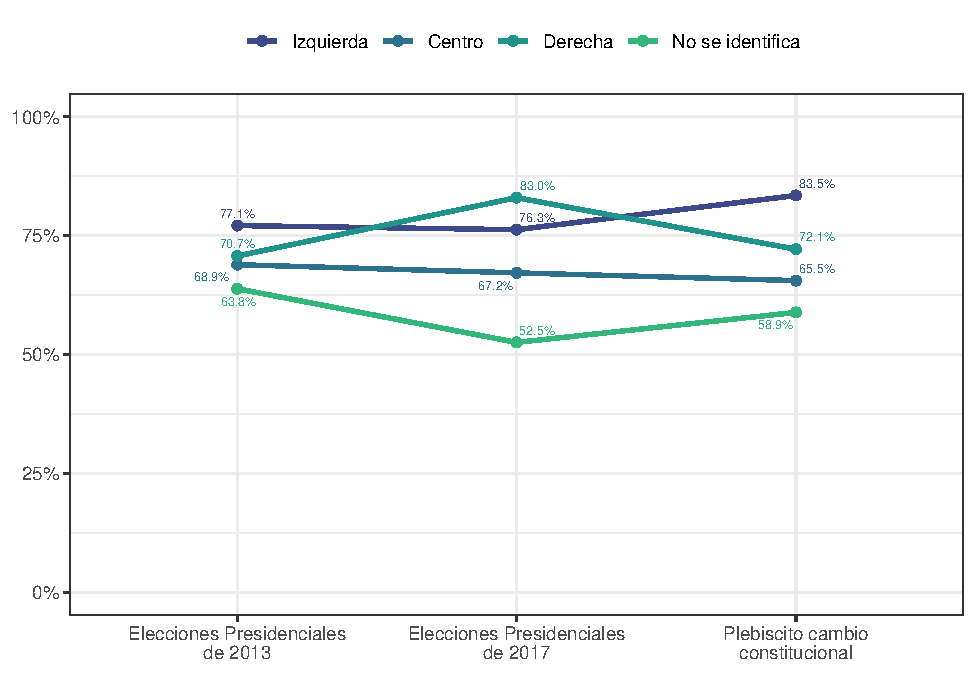
\includegraphics{reporte-elsoc_files/figure-latex/particip-elect-id-1} 

}

\caption{Sí Participa en Elecciones según Identificación Política}\label{fig:particip-elect-id}
\end{figure}

\begin{Shaded}
\begin{Highlighting}[]
\NormalTok{datos.g11}\FloatTok{.5} \OtherTok{\textless{}{-}}\NormalTok{ elsoc\_long\_2016\_2021 }\SpecialCharTok{\%\textgreater{}\%} 
  \FunctionTok{filter}\NormalTok{(ola }\SpecialCharTok{==} \DecValTok{5} \SpecialCharTok{\&}\NormalTok{ tipo\_atricion }\SpecialCharTok{==} \DecValTok{1} \SpecialCharTok{\&} \SpecialCharTok{!}\NormalTok{c44 }\SpecialCharTok{\%in\%} \FunctionTok{c}\NormalTok{(}\DecValTok{3}\NormalTok{,}\DecValTok{4}\NormalTok{, }\SpecialCharTok{{-}}\DecValTok{888}\NormalTok{, }\SpecialCharTok{{-}}\DecValTok{999}\NormalTok{) }\SpecialCharTok{\&} \SpecialCharTok{!}\NormalTok{c15 }\SpecialCharTok{\%in\%} \FunctionTok{c}\NormalTok{(}\SpecialCharTok{{-}}\DecValTok{888}\NormalTok{, }\SpecialCharTok{{-}}\DecValTok{999}\NormalTok{)) }\SpecialCharTok{\%\textgreater{}\%} 
  \FunctionTok{mutate}\NormalTok{(}\AttributeTok{pos\_id =} \FunctionTok{factor}\NormalTok{(car}\SpecialCharTok{::}\FunctionTok{recode}\NormalTok{(c15, }\AttributeTok{recodes =} \StringTok{"0:4 = 1; 5 = 2; 6:10 = 3; 11:12 = 4"}\NormalTok{),}
                         \AttributeTok{levels =} \FunctionTok{c}\NormalTok{(}\DecValTok{1}\NormalTok{, }\DecValTok{2}\NormalTok{, }\DecValTok{3}\NormalTok{, }\DecValTok{4}\NormalTok{),}
                         \AttributeTok{labels =} \FunctionTok{c}\NormalTok{(}\StringTok{\textquotesingle{}Izquierda\textquotesingle{}}\NormalTok{, }\StringTok{"Centro"}\NormalTok{, }\StringTok{"Derecha"}\NormalTok{, }\StringTok{"No se identifica"}\NormalTok{))) }\SpecialCharTok{\%\textgreater{}\%}
  \FunctionTok{prop}\NormalTok{(c44, }\AttributeTok{by =} \FunctionTok{c}\NormalTok{(pos\_id), }\AttributeTok{na.rm =} \ConstantTok{TRUE}\NormalTok{, }\AttributeTok{vartype =} \ConstantTok{NULL}\NormalTok{) }\SpecialCharTok{\%\textgreater{}\%} 
\NormalTok{  sjlabelled}\SpecialCharTok{::}\FunctionTok{as\_label}\NormalTok{(c44, pos\_id) }

\NormalTok{g11}\FloatTok{.5} \OtherTok{\textless{}{-}}\NormalTok{ datos.g11}\FloatTok{.5} \SpecialCharTok{\%\textgreater{}\%} 
  \FunctionTok{ggplot}\NormalTok{(}\FunctionTok{aes}\NormalTok{(}\AttributeTok{y =}\NormalTok{ prop, }\AttributeTok{x =}\NormalTok{ pos\_id, }\AttributeTok{fill =}\NormalTok{ c44, }
             \AttributeTok{label =} \FunctionTok{as.character}\NormalTok{(scales}\SpecialCharTok{::}\FunctionTok{percent}\NormalTok{(prop, }\AttributeTok{accuracy =}\NormalTok{ .}\DecValTok{1}\NormalTok{)))) }\SpecialCharTok{+} 
  \FunctionTok{theme\_bw}\NormalTok{() }\SpecialCharTok{+} 
  \FunctionTok{geom\_col}\NormalTok{(}\AttributeTok{position =} \StringTok{"Stack"}\NormalTok{) }\SpecialCharTok{+}
  \FunctionTok{scale\_y\_continuous}\NormalTok{(}\AttributeTok{labels =}\NormalTok{ scales}\SpecialCharTok{::}\NormalTok{percent) }\SpecialCharTok{+}
  \FunctionTok{ylab}\NormalTok{(}\AttributeTok{label =} \ConstantTok{NULL}\NormalTok{) }\SpecialCharTok{+}
  \FunctionTok{xlab}\NormalTok{(}\AttributeTok{label =} \ConstantTok{NULL}\NormalTok{) }\SpecialCharTok{+}
  \FunctionTok{scale\_fill\_viridis\_d}\NormalTok{(}\AttributeTok{begin =}\NormalTok{ .}\DecValTok{33}\NormalTok{, }\AttributeTok{end =}\NormalTok{ .}\DecValTok{66}\NormalTok{, }\AttributeTok{direction =} \SpecialCharTok{{-}}\DecValTok{1}\NormalTok{, }\AttributeTok{option =} \StringTok{\textquotesingle{}viridis\textquotesingle{}}\NormalTok{) }\SpecialCharTok{+}
  \FunctionTok{geom\_text}\NormalTok{(}\AttributeTok{position =} \FunctionTok{position\_stack}\NormalTok{(}\AttributeTok{vjust =}\NormalTok{ .}\DecValTok{5}\NormalTok{),}
            \AttributeTok{size=} \FloatTok{2.75}\NormalTok{, }\AttributeTok{color =} \FunctionTok{rep.int}\NormalTok{(}\FunctionTok{c}\NormalTok{(}\StringTok{\textquotesingle{}black\textquotesingle{}}\NormalTok{, }\StringTok{\textquotesingle{}black\textquotesingle{}}\NormalTok{), }\DecValTok{4}\NormalTok{)) }\SpecialCharTok{+} 
  \FunctionTok{theme}\NormalTok{(}\AttributeTok{legend.position =} \StringTok{\textquotesingle{}top\textquotesingle{}}\NormalTok{,}
        \AttributeTok{legend.title =} \FunctionTok{element\_blank}\NormalTok{())}

\NormalTok{g11}\FloatTok{.5}
\end{Highlighting}
\end{Shaded}

\begin{figure}

{\centering 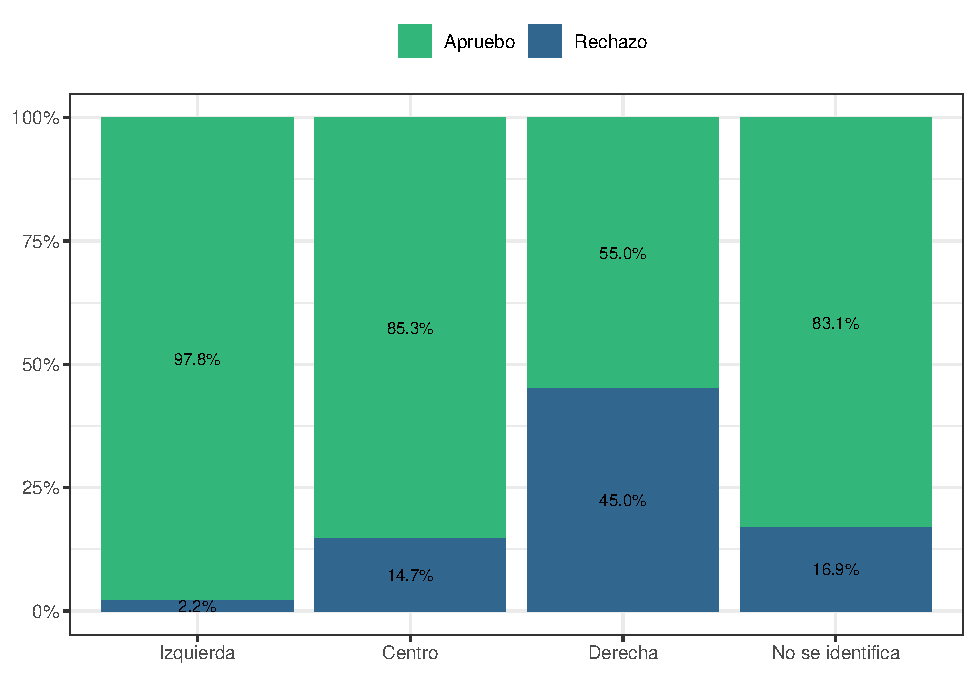
\includegraphics{reporte-elsoc_files/figure-latex/id-pol-voto-1} 

}

\caption{Voto Retrospectivo Plebicito, según Posición Ideológica}\label{fig:id-pol-voto}
\end{figure}

\hypertarget{patrones-de-votaciuxf3n}{%
\section{Patrones de Votación}\label{patrones-de-votaciuxf3n}}

\begin{Shaded}
\begin{Highlighting}[]
\NormalTok{datos.g11}\FloatTok{.6} \OtherTok{\textless{}{-}}\NormalTok{ elsoc\_wide\_2016\_2021 }\SpecialCharTok{\%\textgreater{}\%} 
\NormalTok{  dplyr}\SpecialCharTok{::}\FunctionTok{filter}\NormalTok{(tipo\_atricion }\SpecialCharTok{==} \DecValTok{1} 
                \SpecialCharTok{\&} \SpecialCharTok{!}\NormalTok{c44\_w05 }\SpecialCharTok{\%in\%} \FunctionTok{c}\NormalTok{(}\DecValTok{3}\NormalTok{,}\DecValTok{4}\NormalTok{, }\SpecialCharTok{{-}}\DecValTok{888}\NormalTok{, }\SpecialCharTok{{-}}\DecValTok{999}\NormalTok{)}
                \SpecialCharTok{\&} \SpecialCharTok{!}\NormalTok{c39\_w03 }\SpecialCharTok{\%in\%} \FunctionTok{c}\NormalTok{(}\SpecialCharTok{{-}}\DecValTok{888}\NormalTok{, }\SpecialCharTok{{-}}\DecValTok{999}\NormalTok{) }\SpecialCharTok{\&} \SpecialCharTok{!}\FunctionTok{is.na}\NormalTok{(c44\_w05) }\SpecialCharTok{\&} \SpecialCharTok{!}\FunctionTok{is.na}\NormalTok{(c39\_w03)) }\SpecialCharTok{\%\textgreater{}\%} 
  \FunctionTok{survey\_design\_elsoc}\NormalTok{(}\AttributeTok{weights =} \StringTok{\textquotesingle{}ponderador02\_w05\textquotesingle{}}\NormalTok{) }\SpecialCharTok{\%\textgreater{}\%} 
  \FunctionTok{prop}\NormalTok{(c44\_w05, }\AttributeTok{by =}\NormalTok{ c39\_w03, }\AttributeTok{na.rm =} \ConstantTok{TRUE}\NormalTok{, }\AttributeTok{vartype =} \ConstantTok{NULL}\NormalTok{) }\SpecialCharTok{\%\textgreater{}\%} 
\NormalTok{  sjlabelled}\SpecialCharTok{::}\FunctionTok{as\_label}\NormalTok{(c44\_w05, c39\_w03) }

\NormalTok{g11}\FloatTok{.6} \OtherTok{\textless{}{-}}\NormalTok{ datos.g11}\FloatTok{.6} \SpecialCharTok{\%\textgreater{}\%} 
  \FunctionTok{ggplot}\NormalTok{(}\FunctionTok{aes}\NormalTok{(}\AttributeTok{x =}\NormalTok{ prop, }\AttributeTok{y =}\NormalTok{ c39\_w03, }\AttributeTok{fill =}\NormalTok{ c44\_w05, }
             \AttributeTok{label =} \FunctionTok{as.character}\NormalTok{(scales}\SpecialCharTok{::}\FunctionTok{percent}\NormalTok{(prop, }\AttributeTok{accuracy =}\NormalTok{ .}\DecValTok{1}\NormalTok{)))) }\SpecialCharTok{+} 
  \FunctionTok{theme\_bw}\NormalTok{() }\SpecialCharTok{+} 
  \FunctionTok{geom\_col}\NormalTok{(}\AttributeTok{position =} \StringTok{"Stack"}\NormalTok{) }\SpecialCharTok{+}
  \FunctionTok{scale\_x\_continuous}\NormalTok{(}\AttributeTok{labels =}\NormalTok{ scales}\SpecialCharTok{::}\NormalTok{percent) }\SpecialCharTok{+}
  \FunctionTok{ylab}\NormalTok{(}\AttributeTok{label =} \ConstantTok{NULL}\NormalTok{) }\SpecialCharTok{+}
  \FunctionTok{xlab}\NormalTok{(}\AttributeTok{label =} \ConstantTok{NULL}\NormalTok{) }\SpecialCharTok{+}
  \FunctionTok{scale\_fill\_viridis\_d}\NormalTok{(}\AttributeTok{begin =}\NormalTok{ .}\DecValTok{33}\NormalTok{, }\AttributeTok{end =}\NormalTok{ .}\DecValTok{66}\NormalTok{, }\AttributeTok{direction =} \SpecialCharTok{{-}}\DecValTok{1}\NormalTok{, }\AttributeTok{option =} \StringTok{\textquotesingle{}viridis\textquotesingle{}}\NormalTok{) }\SpecialCharTok{+}
  \FunctionTok{geom\_text}\NormalTok{(}\FunctionTok{aes}\NormalTok{(}\AttributeTok{label =} \FunctionTok{ifelse}\NormalTok{(prop }\SpecialCharTok{\textgreater{}} \FloatTok{0.04}\NormalTok{ , scales}\SpecialCharTok{::}\FunctionTok{percent}\NormalTok{(prop, }\AttributeTok{accuracy =}\NormalTok{ .}\DecValTok{1}\NormalTok{),}\StringTok{""}\NormalTok{)),}
            \AttributeTok{position =} \FunctionTok{position\_stack}\NormalTok{(}\AttributeTok{vjust =}\NormalTok{ .}\DecValTok{5}\NormalTok{),}
            \AttributeTok{show.legend =} \ConstantTok{FALSE}\NormalTok{,}
            \AttributeTok{size =} \FloatTok{2.75}\NormalTok{) }\SpecialCharTok{+} 
  \FunctionTok{theme}\NormalTok{(}\AttributeTok{legend.position =} \StringTok{\textquotesingle{}top\textquotesingle{}}\NormalTok{,}
        \AttributeTok{legend.title =} \FunctionTok{element\_blank}\NormalTok{()) }

\NormalTok{g11}\FloatTok{.6}
\end{Highlighting}
\end{Shaded}

\begin{figure}

{\centering 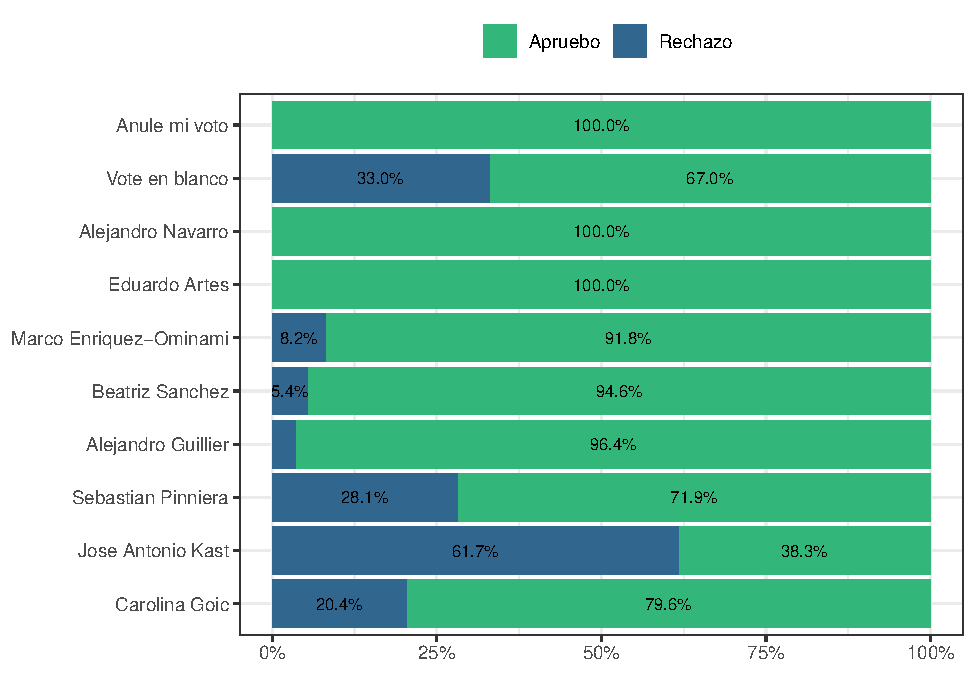
\includegraphics{reporte-elsoc_files/figure-latex/presi-voto-c44-1} 

}

\caption{Voto Retrospectivo Plebicito, según Posición Ideológica}\label{fig:presi-voto-c44}
\end{figure}

\begin{Shaded}
\begin{Highlighting}[]
\NormalTok{datos.g11}\FloatTok{.7} \OtherTok{\textless{}{-}}\NormalTok{ elsoc\_wide\_2016\_2021 }\SpecialCharTok{\%\textgreater{}\%} 
\NormalTok{  dplyr}\SpecialCharTok{::}\FunctionTok{filter}\NormalTok{(tipo\_atricion }\SpecialCharTok{==} \DecValTok{1} 
                \SpecialCharTok{\&} \SpecialCharTok{!}\NormalTok{c45\_w05 }\SpecialCharTok{\%in\%} \FunctionTok{c}\NormalTok{(}\DecValTok{3}\NormalTok{,}\DecValTok{4}\NormalTok{, }\SpecialCharTok{{-}}\DecValTok{888}\NormalTok{, }\SpecialCharTok{{-}}\DecValTok{999}\NormalTok{)}
                \SpecialCharTok{\&} \SpecialCharTok{!}\NormalTok{c39\_w03 }\SpecialCharTok{\%in\%} \FunctionTok{c}\NormalTok{(}\SpecialCharTok{{-}}\DecValTok{888}\NormalTok{, }\SpecialCharTok{{-}}\DecValTok{999}\NormalTok{) }\SpecialCharTok{\&} \SpecialCharTok{!}\FunctionTok{is.na}\NormalTok{(c45\_w05) }\SpecialCharTok{\&} \SpecialCharTok{!}\FunctionTok{is.na}\NormalTok{(c39\_w03)) }\SpecialCharTok{\%\textgreater{}\%} 
  \FunctionTok{survey\_design\_elsoc}\NormalTok{(}\AttributeTok{weights =} \StringTok{\textquotesingle{}ponderador02\_w05\textquotesingle{}}\NormalTok{) }\SpecialCharTok{\%\textgreater{}\%} 
  \FunctionTok{prop}\NormalTok{(c45\_w05, }\AttributeTok{by =}\NormalTok{ c39\_w03, }\AttributeTok{na.rm =} \ConstantTok{TRUE}\NormalTok{, }\AttributeTok{vartype =} \ConstantTok{NULL}\NormalTok{) }\SpecialCharTok{\%\textgreater{}\%} 
\NormalTok{  sjlabelled}\SpecialCharTok{::}\FunctionTok{as\_label}\NormalTok{(c45\_w05, c39\_w03) }

\NormalTok{g11}\FloatTok{.7} \OtherTok{\textless{}{-}}\NormalTok{ datos.g11}\FloatTok{.7} \SpecialCharTok{\%\textgreater{}\%} 
  \FunctionTok{ggplot}\NormalTok{(}\FunctionTok{aes}\NormalTok{(}\AttributeTok{x =}\NormalTok{ prop, }\AttributeTok{y =}\NormalTok{ c39\_w03, }\AttributeTok{fill =}\NormalTok{ c45\_w05, }
             \AttributeTok{label =} \FunctionTok{as.character}\NormalTok{(scales}\SpecialCharTok{::}\FunctionTok{percent}\NormalTok{(prop, }\AttributeTok{accuracy =}\NormalTok{ .}\DecValTok{1}\NormalTok{)))) }\SpecialCharTok{+} 
  \FunctionTok{theme\_bw}\NormalTok{() }\SpecialCharTok{+} 
  \FunctionTok{geom\_col}\NormalTok{(}\AttributeTok{position =} \StringTok{"Stack"}\NormalTok{) }\SpecialCharTok{+}
  \FunctionTok{scale\_x\_continuous}\NormalTok{(}\AttributeTok{labels =}\NormalTok{ scales}\SpecialCharTok{::}\NormalTok{percent) }\SpecialCharTok{+}
  \FunctionTok{ylab}\NormalTok{(}\AttributeTok{label =} \ConstantTok{NULL}\NormalTok{) }\SpecialCharTok{+}
  \FunctionTok{xlab}\NormalTok{(}\AttributeTok{label =} \ConstantTok{NULL}\NormalTok{) }\SpecialCharTok{+}
  \FunctionTok{scale\_fill\_viridis\_d}\NormalTok{(}\AttributeTok{begin =}\NormalTok{ .}\DecValTok{33}\NormalTok{, }\AttributeTok{end =}\NormalTok{ .}\DecValTok{66}\NormalTok{, }\AttributeTok{direction =} \SpecialCharTok{{-}}\DecValTok{1}\NormalTok{, }\AttributeTok{option =} \StringTok{\textquotesingle{}viridis\textquotesingle{}}\NormalTok{) }\SpecialCharTok{+}
  \FunctionTok{geom\_text}\NormalTok{(}\FunctionTok{aes}\NormalTok{(}\AttributeTok{label =} \FunctionTok{ifelse}\NormalTok{(prop }\SpecialCharTok{\textgreater{}} \FloatTok{0.04}\NormalTok{ , scales}\SpecialCharTok{::}\FunctionTok{percent}\NormalTok{(prop, }\AttributeTok{accuracy =}\NormalTok{ .}\DecValTok{1}\NormalTok{),}\StringTok{""}\NormalTok{)),}
            \AttributeTok{position =} \FunctionTok{position\_stack}\NormalTok{(}\AttributeTok{vjust =}\NormalTok{ .}\DecValTok{5}\NormalTok{),}
            \AttributeTok{show.legend =} \ConstantTok{FALSE}\NormalTok{,}
            \AttributeTok{size =} \FloatTok{2.75}\NormalTok{,}
            \AttributeTok{color =} \FunctionTok{rep.int}\NormalTok{(}\FunctionTok{c}\NormalTok{(}\StringTok{\textquotesingle{}black\textquotesingle{}}\NormalTok{, }\StringTok{\textquotesingle{}white\textquotesingle{}}\NormalTok{), }\DecValTok{10}\NormalTok{)) }\SpecialCharTok{+} 
  \FunctionTok{theme}\NormalTok{(}\AttributeTok{legend.position =} \StringTok{\textquotesingle{}top\textquotesingle{}}\NormalTok{,}
        \AttributeTok{legend.title =} \FunctionTok{element\_blank}\NormalTok{()) }

\NormalTok{g11}\FloatTok{.7}
\end{Highlighting}
\end{Shaded}

\begin{figure}

{\centering 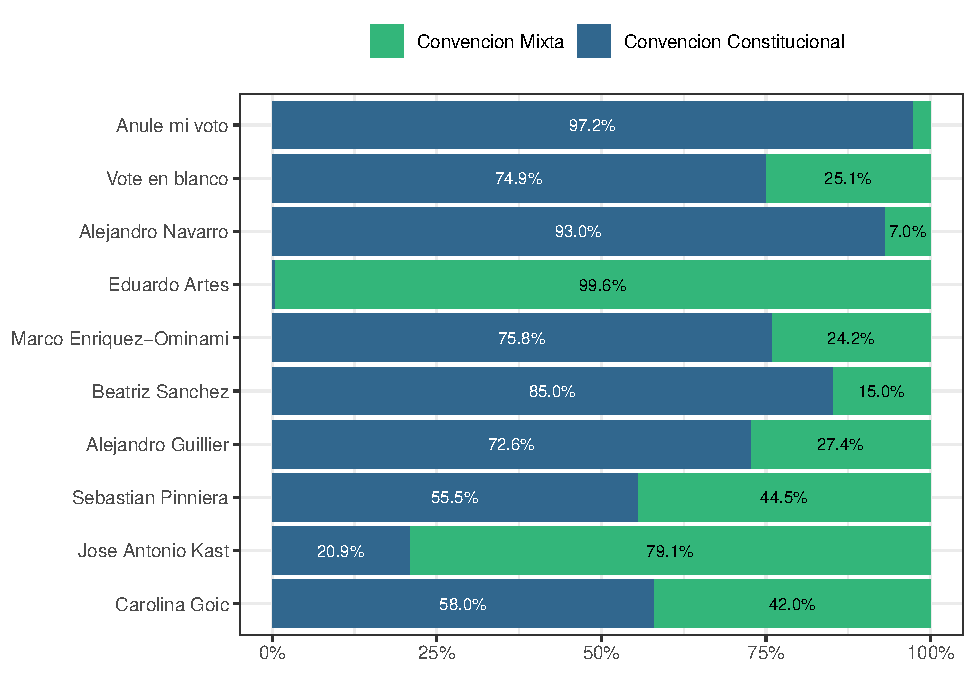
\includegraphics{reporte-elsoc_files/figure-latex/presi-voto-c45-1} 

}

\caption{Voto Retrospectivo Plebicito, según Posición Ideológica}\label{fig:presi-voto-c45}
\end{figure}

\begin{Shaded}
\begin{Highlighting}[]
\NormalTok{datos.}\FloatTok{11.7} \OtherTok{\textless{}{-}}\NormalTok{ elsoc\_wide\_2016\_2021 }\SpecialCharTok{\%\textgreater{}\%} 
  \FunctionTok{filter}\NormalTok{(tipo\_atricion }\SpecialCharTok{==} \DecValTok{1} \SpecialCharTok{\&} \SpecialCharTok{!}\NormalTok{c43\_w05 }\SpecialCharTok{\%in\%} \FunctionTok{c}\NormalTok{(}\DecValTok{3}\NormalTok{, }\SpecialCharTok{{-}}\DecValTok{888}\NormalTok{, }\SpecialCharTok{{-}}\DecValTok{999}\NormalTok{) }\SpecialCharTok{\&} 
           \SpecialCharTok{!}\NormalTok{c11\_w03 }\SpecialCharTok{\%in\%} \FunctionTok{c}\NormalTok{(}\DecValTok{3}\NormalTok{, }\SpecialCharTok{{-}}\DecValTok{888}\NormalTok{, }\SpecialCharTok{{-}}\DecValTok{999}\NormalTok{)) }\SpecialCharTok{\%\textgreater{}\%} 
  \FunctionTok{survey\_design\_elsoc}\NormalTok{(}\AttributeTok{weights =} \StringTok{\textquotesingle{}ponderador02\_w05\textquotesingle{}}\NormalTok{) }\SpecialCharTok{\%\textgreater{}\%} 
  \FunctionTok{prop}\NormalTok{(c43\_w05, }\AttributeTok{by =}\NormalTok{ c11\_w03) }\SpecialCharTok{\%\textgreater{}\%} 
\NormalTok{  sjlabelled}\SpecialCharTok{::}\FunctionTok{as\_label}\NormalTok{(c43\_w05, c11\_w03)}

\NormalTok{datos.}\FloatTok{11.7} \SpecialCharTok{\%\textgreater{}\%} 
  \FunctionTok{ggplot}\NormalTok{(}\FunctionTok{aes}\NormalTok{(}\AttributeTok{y =}\NormalTok{ prop, }\AttributeTok{x =}\NormalTok{ c11\_w03, }\AttributeTok{fill =}\NormalTok{ c43\_w05, }
             \AttributeTok{label =}\NormalTok{ scales}\SpecialCharTok{::}\FunctionTok{percent}\NormalTok{(prop, }\AttributeTok{accuracy =}\NormalTok{ .}\DecValTok{1}\NormalTok{))) }\SpecialCharTok{+} 
  \FunctionTok{theme\_bw}\NormalTok{() }\SpecialCharTok{+} 
  \FunctionTok{geom\_col}\NormalTok{(}\AttributeTok{position =} \StringTok{"Stack"}\NormalTok{) }\SpecialCharTok{+}
  \FunctionTok{scale\_y\_continuous}\NormalTok{(}\AttributeTok{labels =}\NormalTok{ scales}\SpecialCharTok{::}\NormalTok{percent) }\SpecialCharTok{+} 
  \FunctionTok{ylab}\NormalTok{(}\AttributeTok{label =} \ConstantTok{NULL}\NormalTok{) }\SpecialCharTok{+}
  \FunctionTok{xlab}\NormalTok{(}\AttributeTok{label =} \StringTok{"Participación Electoral en 2017"}\NormalTok{) }\SpecialCharTok{+}
  \FunctionTok{scale\_fill\_viridis\_d}\NormalTok{(}\AttributeTok{begin =}\NormalTok{ .}\DecValTok{33}\NormalTok{, }\AttributeTok{end =}\NormalTok{ .}\DecValTok{66}\NormalTok{, }\AttributeTok{direction =} \SpecialCharTok{{-}}\DecValTok{1}\NormalTok{, }\AttributeTok{option =} \StringTok{\textquotesingle{}viridis\textquotesingle{}}\NormalTok{) }\SpecialCharTok{+} 
  \FunctionTok{geom\_text}\NormalTok{(}\AttributeTok{position =} \FunctionTok{position\_stack}\NormalTok{(}\AttributeTok{vjust =}\NormalTok{ .}\DecValTok{5}\NormalTok{),}
            \AttributeTok{show.legend =} \ConstantTok{FALSE}\NormalTok{,}
            \AttributeTok{size =} \FloatTok{2.75}\NormalTok{,}
            \AttributeTok{color =} \FunctionTok{rep}\NormalTok{(}\FunctionTok{c}\NormalTok{(}\StringTok{\textquotesingle{}black\textquotesingle{}}\NormalTok{, }\StringTok{\textquotesingle{}white\textquotesingle{}}\NormalTok{), }\DecValTok{2}\NormalTok{)) }\SpecialCharTok{+} 
  \FunctionTok{theme}\NormalTok{(}\AttributeTok{legend.position =} \StringTok{\textquotesingle{}top\textquotesingle{}}\NormalTok{,}
        \AttributeTok{legend.title =} \FunctionTok{element\_blank}\NormalTok{()) }
\end{Highlighting}
\end{Shaded}

\begin{figure}

{\centering 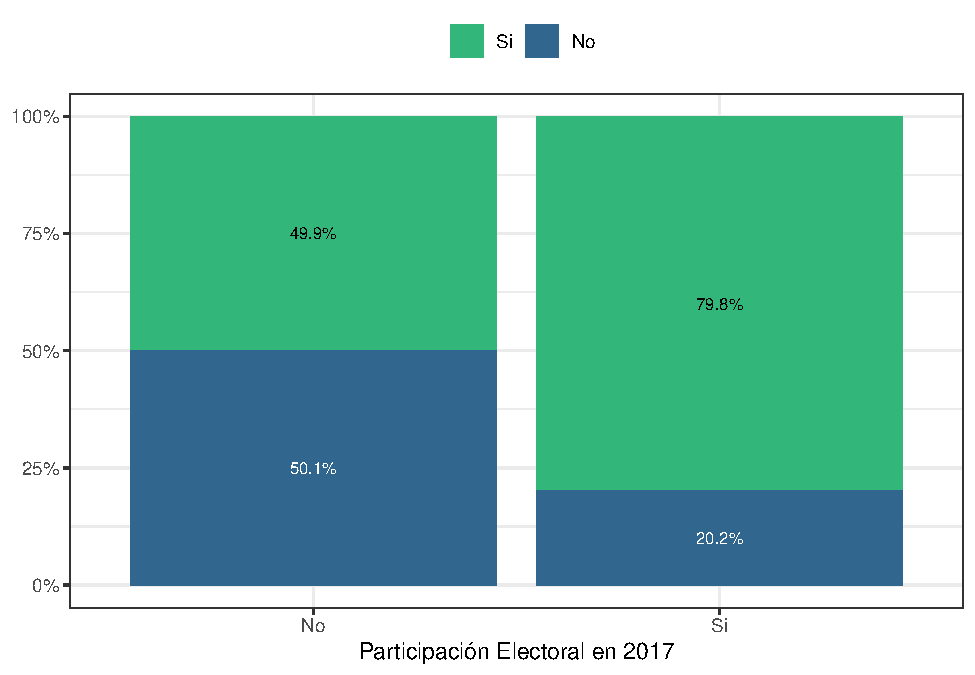
\includegraphics{reporte-elsoc_files/figure-latex/2020-vs-2021-1} 

}

\caption{Participación Electoral 2021, según la Participación en 2017}\label{fig:2020-vs-2021}
\end{figure}

\begin{Shaded}
\begin{Highlighting}[]
\CommentTok{\#grafico y caracterización pendiente}
\NormalTok{elsoc\_wide\_2016\_2021 }\SpecialCharTok{\%\textgreater{}\%} 
  \FunctionTok{filter}\NormalTok{(tipo\_atricion }\SpecialCharTok{==} \DecValTok{1} \SpecialCharTok{\&} \SpecialCharTok{!}\NormalTok{c11\_w03 }\SpecialCharTok{\%in\%} \FunctionTok{c}\NormalTok{(}\SpecialCharTok{{-}}\DecValTok{888}\NormalTok{, }\SpecialCharTok{{-}}\DecValTok{999}\NormalTok{, }\DecValTok{3}\NormalTok{) }\SpecialCharTok{\&} \SpecialCharTok{!}\NormalTok{c43\_w05 }\SpecialCharTok{\%in\%} \FunctionTok{c}\NormalTok{(}\SpecialCharTok{{-}}\DecValTok{888}\NormalTok{, }\SpecialCharTok{{-}}\DecValTok{999}\NormalTok{, }\DecValTok{3}\NormalTok{) }\SpecialCharTok{\&}
           \SpecialCharTok{!}\NormalTok{c15\_w03 }\SpecialCharTok{\%in\%} \FunctionTok{c}\NormalTok{(}\SpecialCharTok{{-}}\DecValTok{888}\NormalTok{, }\SpecialCharTok{{-}}\DecValTok{999}\NormalTok{)) }\SpecialCharTok{\%\textgreater{}\%} 
  \FunctionTok{mutate}\NormalTok{(}\AttributeTok{cambio\_participa =} \FunctionTok{factor}\NormalTok{(}\FunctionTok{case\_when}\NormalTok{(c11\_w03 }\SpecialCharTok{==} \DecValTok{1} \SpecialCharTok{\&}\NormalTok{ c43\_w05 }\SpecialCharTok{==} \DecValTok{2} \SpecialCharTok{\textasciitilde{}} \DecValTok{1}\NormalTok{,}
\NormalTok{                                             c11\_w03 }\SpecialCharTok{==} \DecValTok{1} \SpecialCharTok{\&}\NormalTok{ c43\_w05 }\SpecialCharTok{==} \DecValTok{1} \SpecialCharTok{\textasciitilde{}} \DecValTok{2}\NormalTok{,}
\NormalTok{                                             c11\_w03 }\SpecialCharTok{==} \DecValTok{2} \SpecialCharTok{\&}\NormalTok{ c43\_w05 }\SpecialCharTok{==} \DecValTok{2} \SpecialCharTok{\textasciitilde{}} \DecValTok{3}\NormalTok{,}
\NormalTok{                                             c11\_w03 }\SpecialCharTok{==} \DecValTok{2} \SpecialCharTok{\&}\NormalTok{ c43\_w05 }\SpecialCharTok{==} \DecValTok{1} \SpecialCharTok{\textasciitilde{}} \DecValTok{4}\NormalTok{),}
                                   \AttributeTok{labels =} \FunctionTok{c}\NormalTok{(}\StringTok{\textquotesingle{}Se mantiene no votando\textquotesingle{}}\NormalTok{, }\StringTok{\textquotesingle{}Cambia a votar\textquotesingle{}}\NormalTok{,}
                                              \StringTok{\textquotesingle{}Cambia a No Votar\textquotesingle{}}\NormalTok{, }\StringTok{\textquotesingle{}Se mantiene votando\textquotesingle{}}\NormalTok{)),}
         \AttributeTok{pos\_id\_w03 =} \FunctionTok{factor}\NormalTok{(car}\SpecialCharTok{::}\FunctionTok{recode}\NormalTok{(c15\_w03, }\StringTok{"0:4 = 1; 5 = 2; 6:10 = 3; 11:12 = 4"}\NormalTok{),}
                         \AttributeTok{levels =} \FunctionTok{c}\NormalTok{(}\DecValTok{1}\NormalTok{, }\DecValTok{2}\NormalTok{, }\DecValTok{3}\NormalTok{, }\DecValTok{4}\NormalTok{),}
                         \AttributeTok{labels =} \FunctionTok{c}\NormalTok{(}\StringTok{\textquotesingle{}Izquierda\textquotesingle{}}\NormalTok{, }\StringTok{"Centro"}\NormalTok{, }\StringTok{"Derecha"}\NormalTok{, }\StringTok{"No se identifica"}\NormalTok{))) }\SpecialCharTok{\%\textgreater{}\%} 
\NormalTok{  elsoc}\SpecialCharTok{::}\FunctionTok{survey\_design\_elsoc}\NormalTok{(}\AttributeTok{weights =} \StringTok{\textquotesingle{}ponderador02\_w05\textquotesingle{}}\NormalTok{) }\SpecialCharTok{\%\textgreater{}\%} 
  \FunctionTok{prop}\NormalTok{(cambio\_participa, }\AttributeTok{by =}\NormalTok{ pos\_id\_w03, }\AttributeTok{na.rm =} \ConstantTok{TRUE}\NormalTok{) }\SpecialCharTok{\%\textgreater{}\%} 
  \FunctionTok{ggplot}\NormalTok{(}\FunctionTok{aes}\NormalTok{(}\AttributeTok{y =}\NormalTok{ prop, }\AttributeTok{x =}\NormalTok{ pos\_id\_w03, }\AttributeTok{fill =}\NormalTok{ cambio\_participa, }
             \AttributeTok{label =}\NormalTok{ scales}\SpecialCharTok{::}\FunctionTok{percent}\NormalTok{(prop, }\AttributeTok{accuracy =}\NormalTok{ .}\DecValTok{1}\NormalTok{))) }\SpecialCharTok{+} 
  \FunctionTok{theme\_bw}\NormalTok{() }\SpecialCharTok{+} 
  \FunctionTok{geom\_col}\NormalTok{(}\AttributeTok{position =} \StringTok{"Stack"}\NormalTok{) }\SpecialCharTok{+}
  \FunctionTok{scale\_y\_continuous}\NormalTok{(}\AttributeTok{labels =}\NormalTok{ scales}\SpecialCharTok{::}\NormalTok{percent) }\SpecialCharTok{+} 
  \FunctionTok{ylab}\NormalTok{(}\AttributeTok{label =} \ConstantTok{NULL}\NormalTok{) }\SpecialCharTok{+}
  \FunctionTok{xlab}\NormalTok{(}\AttributeTok{label =} \StringTok{"Posición ideológica en 2017"}\NormalTok{) }\SpecialCharTok{+}
  \FunctionTok{scale\_fill\_viridis\_d}\NormalTok{(}\AttributeTok{begin =}\NormalTok{ .}\DecValTok{33}\NormalTok{, }\AttributeTok{end =}\NormalTok{ .}\DecValTok{66}\NormalTok{, }\AttributeTok{direction =} \SpecialCharTok{{-}}\DecValTok{1}\NormalTok{, }\AttributeTok{option =} \StringTok{\textquotesingle{}viridis\textquotesingle{}}\NormalTok{) }\SpecialCharTok{+} 
  \FunctionTok{geom\_text}\NormalTok{(}\AttributeTok{position =} \FunctionTok{position\_stack}\NormalTok{(}\AttributeTok{vjust =}\NormalTok{ .}\DecValTok{5}\NormalTok{),}
            \AttributeTok{show.legend =} \ConstantTok{FALSE}\NormalTok{,}
            \AttributeTok{size =} \FloatTok{2.75}\NormalTok{,}
            \AttributeTok{color =} \FunctionTok{rep}\NormalTok{(}\FunctionTok{c}\NormalTok{(}\StringTok{\textquotesingle{}black\textquotesingle{}}\NormalTok{, }\StringTok{\textquotesingle{}black\textquotesingle{}}\NormalTok{, }\StringTok{\textquotesingle{}white\textquotesingle{}}\NormalTok{, }\StringTok{\textquotesingle{}white\textquotesingle{}}\NormalTok{), }\DecValTok{4}\NormalTok{)) }\SpecialCharTok{+} 
  \FunctionTok{theme}\NormalTok{(}\AttributeTok{legend.position =} \StringTok{\textquotesingle{}top\textquotesingle{}}\NormalTok{,}
        \AttributeTok{legend.title =} \FunctionTok{element\_blank}\NormalTok{())}
\end{Highlighting}
\end{Shaded}

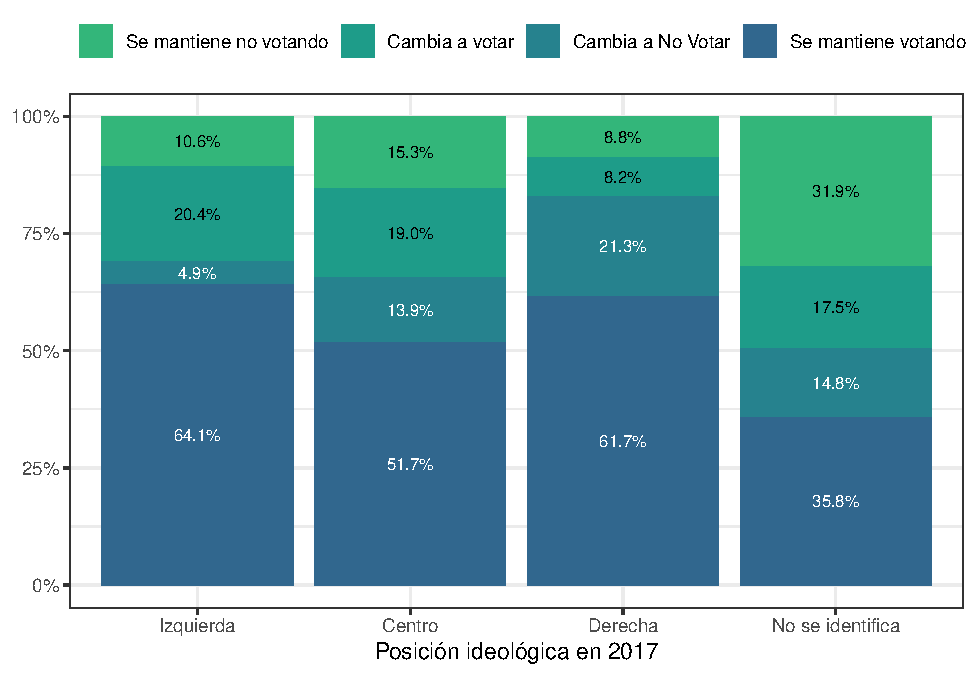
\includegraphics{reporte-elsoc_files/figure-latex/cambio_participa-1.pdf}

\hypertarget{conflicto-y-cohesiuxf3n-territorial-en-pandemia}{%
\chapter{Conflicto y cohesión territorial en pandemia}\label{conflicto-y-cohesiuxf3n-territorial-en-pandemia}}

\hypertarget{conflictividad-barrial}{%
\section{Conflictividad barrial}\label{conflictividad-barrial}}

\begin{Shaded}
\begin{Highlighting}[]
\NormalTok{datos.}\FloatTok{8.1} \OtherTok{\textless{}{-}}\NormalTok{ elsoc\_long\_2016\_2021 }\SpecialCharTok{\%\textgreater{}\%} 
  \FunctionTok{filter}\NormalTok{(tipo\_atricion }\SpecialCharTok{==} \DecValTok{1} \SpecialCharTok{\&}\NormalTok{ muestra }\SpecialCharTok{==} \DecValTok{1} \SpecialCharTok{\&} \SpecialCharTok{!}\NormalTok{t11\_01 }\SpecialCharTok{\%in\%} \FunctionTok{c}\NormalTok{(}\SpecialCharTok{{-}}\DecValTok{888}\NormalTok{, }\SpecialCharTok{{-}}\DecValTok{999}\NormalTok{) }\SpecialCharTok{\&}
           \SpecialCharTok{!}\NormalTok{t11\_02 }\SpecialCharTok{\%in\%} \FunctionTok{c}\NormalTok{(}\SpecialCharTok{{-}}\DecValTok{888}\NormalTok{, }\SpecialCharTok{{-}}\DecValTok{999}\NormalTok{) }\SpecialCharTok{\&} \SpecialCharTok{!}\NormalTok{t11\_03 }\SpecialCharTok{\%in\%} \FunctionTok{c}\NormalTok{(}\SpecialCharTok{{-}}\DecValTok{888}\NormalTok{, }\SpecialCharTok{{-}}\DecValTok{999}\NormalTok{) }\SpecialCharTok{\&} \SpecialCharTok{!}\NormalTok{t11\_04 }\SpecialCharTok{\%in\%} \FunctionTok{c}\NormalTok{(}\SpecialCharTok{{-}}\DecValTok{888}\NormalTok{, }\SpecialCharTok{{-}}\DecValTok{999}\NormalTok{)) }\SpecialCharTok{\%\textgreater{}\%} 
  \FunctionTok{mutate}\NormalTok{(}\AttributeTok{barrio\_confli =}\NormalTok{ (t11\_01 }\SpecialCharTok{+}\NormalTok{ t11\_02 }\SpecialCharTok{+}\NormalTok{ t11\_03 }\SpecialCharTok{+}\NormalTok{ t11\_04)}\SpecialCharTok{/}\DecValTok{4}\NormalTok{) }\SpecialCharTok{\%\textgreater{}\%}
  \FunctionTok{mutate}\NormalTok{(}\AttributeTok{barrio\_confli\_rec =} \FunctionTok{factor}\NormalTok{(}\FunctionTok{cut}\NormalTok{(barrio\_confli, }\AttributeTok{breaks =} \FunctionTok{c}\NormalTok{(}\DecValTok{0}\NormalTok{,}\DecValTok{1}\NormalTok{,}\FloatTok{2.75}\NormalTok{,}\DecValTok{5}\NormalTok{)),}
         \AttributeTok{labels =} \FunctionTok{c}\NormalTok{(}\StringTok{"Nunca"}\NormalTok{,}\StringTok{"Pocas o algunas veces"}\NormalTok{,}\StringTok{"Muchas veces o siempre"}\NormalTok{))) }\SpecialCharTok{\%\textgreater{}\%}
\NormalTok{  sjlabelled}\SpecialCharTok{::}\FunctionTok{as\_label}\NormalTok{(ola) }\SpecialCharTok{\%\textgreater{}\%} 
  \FunctionTok{prop}\NormalTok{(}\AttributeTok{x =}\NormalTok{ barrio\_confli\_rec, }\AttributeTok{by =}\NormalTok{ ola, }\AttributeTok{na.rm =} \ConstantTok{TRUE}\NormalTok{)}

\NormalTok{g8}\FloatTok{.1} \OtherTok{\textless{}{-}}\NormalTok{ datos.}\FloatTok{8.1} \SpecialCharTok{\%\textgreater{}\%} 
  \FunctionTok{ggplot}\NormalTok{(}\FunctionTok{aes}\NormalTok{(}\AttributeTok{y =}\NormalTok{ prop, }\AttributeTok{x =}\NormalTok{ ola, }\AttributeTok{fill =}\NormalTok{ barrio\_confli\_rec, }
             \AttributeTok{label =} \FunctionTok{as.character}\NormalTok{(scales}\SpecialCharTok{::}\FunctionTok{percent}\NormalTok{(prop, }\AttributeTok{accuracy =}\NormalTok{ .}\DecValTok{1}\NormalTok{)))) }\SpecialCharTok{+} 
  \FunctionTok{theme\_bw}\NormalTok{() }\SpecialCharTok{+} 
  \FunctionTok{geom\_col}\NormalTok{(}\AttributeTok{position =} \StringTok{\textquotesingle{}Stack\textquotesingle{}}\NormalTok{) }\SpecialCharTok{+}
  \FunctionTok{ylab}\NormalTok{(}\AttributeTok{label =} \ConstantTok{NULL}\NormalTok{) }\SpecialCharTok{+}
  \FunctionTok{xlab}\NormalTok{(}\AttributeTok{label =} \ConstantTok{NULL}\NormalTok{) }\SpecialCharTok{+}
  \FunctionTok{scale\_fill\_viridis\_d}\NormalTok{(}\AttributeTok{begin =}\NormalTok{ .}\DecValTok{11}\NormalTok{, }\AttributeTok{end =}\NormalTok{ .}\DecValTok{88}\NormalTok{, }\AttributeTok{direction =} \SpecialCharTok{{-}}\DecValTok{1}\NormalTok{, }\AttributeTok{option =} \StringTok{\textquotesingle{}viridis\textquotesingle{}}\NormalTok{) }\SpecialCharTok{+}
  \FunctionTok{geom\_text}\NormalTok{(}\AttributeTok{position =} \FunctionTok{position\_stack}\NormalTok{(}\AttributeTok{vjust =}\NormalTok{ .}\DecValTok{5}\NormalTok{),}
            \AttributeTok{size=} \FloatTok{2.75}\NormalTok{, }\AttributeTok{color =} \FunctionTok{rep}\NormalTok{(}\FunctionTok{c}\NormalTok{(}\StringTok{\textquotesingle{}black\textquotesingle{}}\NormalTok{, }\StringTok{\textquotesingle{}white\textquotesingle{}}\NormalTok{, }\StringTok{\textquotesingle{}white\textquotesingle{}}\NormalTok{), }\DecValTok{5}\NormalTok{)) }\SpecialCharTok{+} 
  \FunctionTok{theme}\NormalTok{(}\AttributeTok{legend.position =} \StringTok{\textquotesingle{}top\textquotesingle{}}\NormalTok{, }\AttributeTok{legend.title =} \FunctionTok{element\_blank}\NormalTok{())}
\NormalTok{g8}\FloatTok{.1}
\end{Highlighting}
\end{Shaded}

\begin{figure}

{\centering 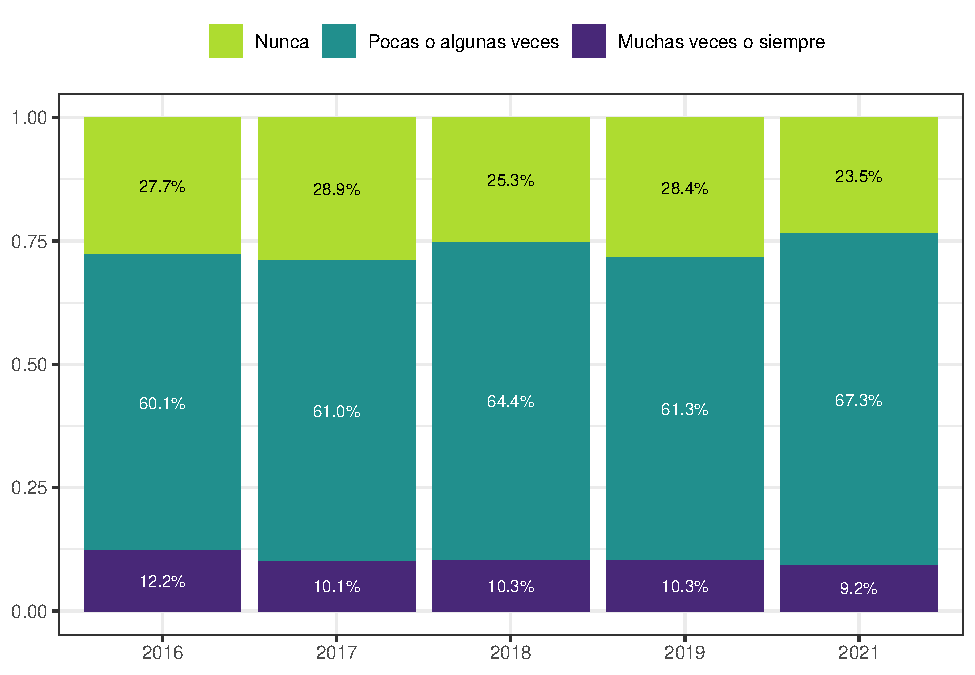
\includegraphics{reporte-elsoc_files/figure-latex/confli-olas-1} 

}

\caption{¿Con qué frecuencia usted/alguien de su hogar se ha molestado o incomodado por problemas con sus vecinos? según ola de estudio }\label{fig:confli-olas}
\end{figure}

\begin{Shaded}
\begin{Highlighting}[]
\NormalTok{elsoc\_diseno }\OtherTok{\textless{}{-}}\NormalTok{ elsoc\_long\_2016\_2021 }\SpecialCharTok{\%\textgreater{}\%} 
  \FunctionTok{filter}\NormalTok{(tipo\_atricion }\SpecialCharTok{==} \DecValTok{1} \SpecialCharTok{\&}\NormalTok{ muestra }\SpecialCharTok{==} \DecValTok{1} \SpecialCharTok{\&}\NormalTok{ ola }\SpecialCharTok{\%in\%} \FunctionTok{c}\NormalTok{(}\DecValTok{4}\NormalTok{,}\DecValTok{5}\NormalTok{) }\SpecialCharTok{\&} \SpecialCharTok{!}\NormalTok{t11\_01 }\SpecialCharTok{\%in\%} \FunctionTok{c}\NormalTok{(}\SpecialCharTok{{-}}\DecValTok{888}\NormalTok{, }\SpecialCharTok{{-}}\DecValTok{999}\NormalTok{) }\SpecialCharTok{\&}
           \SpecialCharTok{!}\NormalTok{t11\_02 }\SpecialCharTok{\%in\%} \FunctionTok{c}\NormalTok{(}\SpecialCharTok{{-}}\DecValTok{888}\NormalTok{, }\SpecialCharTok{{-}}\DecValTok{999}\NormalTok{) }\SpecialCharTok{\&} \SpecialCharTok{!}\NormalTok{t11\_03 }\SpecialCharTok{\%in\%} \FunctionTok{c}\NormalTok{(}\SpecialCharTok{{-}}\DecValTok{888}\NormalTok{, }\SpecialCharTok{{-}}\DecValTok{999}\NormalTok{) }\SpecialCharTok{\&} \SpecialCharTok{!}\NormalTok{t11\_04 }\SpecialCharTok{\%in\%} \FunctionTok{c}\NormalTok{(}\SpecialCharTok{{-}}\DecValTok{888}\NormalTok{, }\SpecialCharTok{{-}}\DecValTok{999}\NormalTok{)) }\SpecialCharTok{\%\textgreater{}\%} 
  \FunctionTok{mutate}\NormalTok{(}\AttributeTok{barrio\_confli =}\NormalTok{ (t11\_01 }\SpecialCharTok{+}\NormalTok{ t11\_02 }\SpecialCharTok{+}\NormalTok{ t11\_03 }\SpecialCharTok{+}\NormalTok{ t11\_04)}\SpecialCharTok{/}\DecValTok{4}\NormalTok{) }\SpecialCharTok{\%\textgreater{}\%}
  \FunctionTok{mutate}\NormalTok{(}\AttributeTok{barrio\_confli\_rec =} \FunctionTok{factor}\NormalTok{(}\FunctionTok{cut}\NormalTok{(barrio\_confli, }\AttributeTok{breaks =} \FunctionTok{c}\NormalTok{(}\DecValTok{0}\NormalTok{,}\DecValTok{1}\NormalTok{,}\FloatTok{2.75}\NormalTok{,}\DecValTok{5}\NormalTok{)),}
         \AttributeTok{labels =} \FunctionTok{c}\NormalTok{(}\StringTok{"Nunca"}\NormalTok{,}\StringTok{"Pocas o algunas veces"}\NormalTok{,}\StringTok{"Muchas veces o siempre"}\NormalTok{))) }\SpecialCharTok{\%\textgreater{}\%}
\NormalTok{  sjlabelled}\SpecialCharTok{::}\FunctionTok{as\_label}\NormalTok{(ola) }\SpecialCharTok{\%\textgreater{}\%} 
  \FunctionTok{survey\_design\_elsoc}\NormalTok{()}

\NormalTok{datos.}\FloatTok{8.2} \OtherTok{\textless{}{-}} \FunctionTok{data.frame}\NormalTok{((}\FunctionTok{svytable}\NormalTok{(}\SpecialCharTok{\textasciitilde{}}\NormalTok{barrio\_confli\_rec }\SpecialCharTok{+}\NormalTok{ ola }\SpecialCharTok{+}\NormalTok{ idencuesta, elsoc\_diseno, }\AttributeTok{round =}\NormalTok{ F))) }\SpecialCharTok{\%\textgreater{}\%} 
\NormalTok{  dplyr}\SpecialCharTok{::}\FunctionTok{filter}\NormalTok{(Freq}\SpecialCharTok{\textgreater{}}\DecValTok{0}\NormalTok{)  }\SpecialCharTok{\%\textgreater{}\%} 
  \FunctionTok{group\_by}\NormalTok{(ola) }\SpecialCharTok{\%\textgreater{}\%} \FunctionTok{mutate}\NormalTok{(}\AttributeTok{prop=}\NormalTok{Freq}\SpecialCharTok{/}\FunctionTok{sum}\NormalTok{(Freq)) }\SpecialCharTok{\%\textgreater{}\%}  
  \FunctionTok{drop\_na}\NormalTok{()}

\NormalTok{etiquetas.}\FloatTok{8.2} \OtherTok{\textless{}{-}} \FunctionTok{data.frame}\NormalTok{((}\FunctionTok{svytable}\NormalTok{(}\SpecialCharTok{\textasciitilde{}}\NormalTok{barrio\_confli\_rec }\SpecialCharTok{+}\NormalTok{ ola, elsoc\_diseno, }\AttributeTok{round =}\NormalTok{ F))) }\SpecialCharTok{\%\textgreater{}\%} 
  \FunctionTok{group\_by}\NormalTok{(ola) }\SpecialCharTok{\%\textgreater{}\%} \FunctionTok{mutate}\NormalTok{(}\AttributeTok{prop=}\NormalTok{Freq}\SpecialCharTok{/}\FunctionTok{sum}\NormalTok{(Freq)) }\SpecialCharTok{\%\textgreater{}\%} \FunctionTok{mutate}\NormalTok{(}\AttributeTok{idencuesta =} \DecValTok{1}\NormalTok{) }\SpecialCharTok{\%\textgreater{}\%} 
  \FunctionTok{drop\_na}\NormalTok{()}

\NormalTok{g8}\FloatTok{.2} \OtherTok{\textless{}{-}} 
  \FunctionTok{ggplot}\NormalTok{(datos.}\FloatTok{8.2}\NormalTok{, }\FunctionTok{aes}\NormalTok{(}\AttributeTok{x =}\NormalTok{ ola, }\AttributeTok{fill =}\NormalTok{ barrio\_confli\_rec, }\AttributeTok{stratum =}\NormalTok{ barrio\_confli\_rec, }
                           \AttributeTok{alluvium =}\NormalTok{ idencuesta, }\AttributeTok{y =}\NormalTok{ prop)) }\SpecialCharTok{+}
\NormalTok{  ggalluvial}\SpecialCharTok{::}\FunctionTok{geom\_flow}\NormalTok{(}\AttributeTok{alpha =}\NormalTok{ .}\DecValTok{66}\NormalTok{) }\SpecialCharTok{+} 
\NormalTok{  ggalluvial}\SpecialCharTok{::}\FunctionTok{geom\_stratum}\NormalTok{(}\AttributeTok{linetype =} \DecValTok{0}\NormalTok{) }\SpecialCharTok{+}
  \FunctionTok{scale\_y\_continuous}\NormalTok{(}\AttributeTok{labels =}\NormalTok{ scales}\SpecialCharTok{::}\NormalTok{percent) }\SpecialCharTok{+} 
  \FunctionTok{ylab}\NormalTok{(}\AttributeTok{label =} \ConstantTok{NULL}\NormalTok{) }\SpecialCharTok{+}
  \FunctionTok{xlab}\NormalTok{(}\AttributeTok{label =} \ConstantTok{NULL}\NormalTok{) }\SpecialCharTok{+} 
  \FunctionTok{theme}\NormalTok{(}\AttributeTok{legend.position =} \StringTok{\textquotesingle{}top\textquotesingle{}}\NormalTok{,}
        \AttributeTok{legend.title =} \FunctionTok{element\_blank}\NormalTok{()) }\SpecialCharTok{+}
  \FunctionTok{scale\_fill\_viridis\_d}\NormalTok{(}\AttributeTok{begin =}\NormalTok{ .}\DecValTok{11}\NormalTok{, }\AttributeTok{end =}\NormalTok{ .}\DecValTok{88}\NormalTok{, }\AttributeTok{direction =} \SpecialCharTok{{-}}\DecValTok{1}\NormalTok{, }\AttributeTok{option =} \StringTok{\textquotesingle{}viridis\textquotesingle{}}\NormalTok{) }\SpecialCharTok{+}
  \FunctionTok{geom\_text}\NormalTok{(}\AttributeTok{data =}\NormalTok{ etiquetas.}\FloatTok{8.2}\NormalTok{, }
            \FunctionTok{aes}\NormalTok{(}\AttributeTok{label =} \FunctionTok{ifelse}\NormalTok{(prop }\SpecialCharTok{\textgreater{}} \FloatTok{0.03}\NormalTok{ , scales}\SpecialCharTok{::}\FunctionTok{percent}\NormalTok{(prop, }\AttributeTok{accuracy =}\NormalTok{ .}\DecValTok{1}\NormalTok{),}\StringTok{""}\NormalTok{)),}
            \AttributeTok{position =} \FunctionTok{position\_stack}\NormalTok{(}\AttributeTok{vjust =}\NormalTok{ .}\DecValTok{5}\NormalTok{),}
            \AttributeTok{show.legend =} \ConstantTok{FALSE}\NormalTok{,}
            \AttributeTok{size =} \FloatTok{2.75}\NormalTok{,}
            \AttributeTok{color =} \FunctionTok{rep}\NormalTok{(}\FunctionTok{c}\NormalTok{(}\StringTok{\textquotesingle{}black\textquotesingle{}}\NormalTok{, }\StringTok{\textquotesingle{}white\textquotesingle{}}\NormalTok{, }\StringTok{\textquotesingle{}white\textquotesingle{}}\NormalTok{),}\DecValTok{2}\NormalTok{))}
\NormalTok{g8}\FloatTok{.2}
\end{Highlighting}
\end{Shaded}

\begin{figure}

{\centering 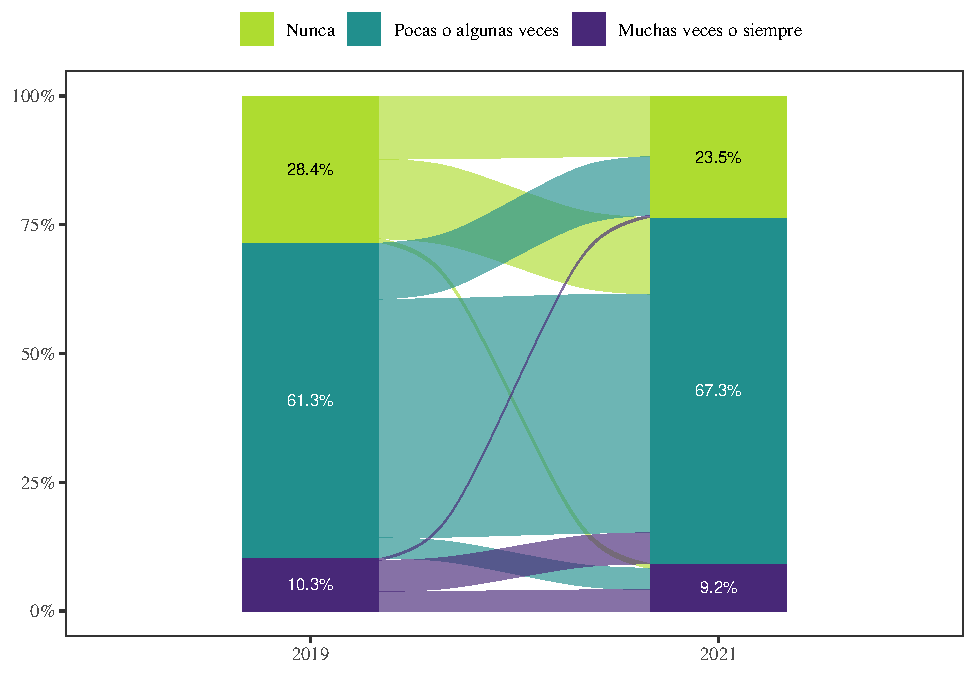
\includegraphics{reporte-elsoc_files/figure-latex/confli-cambio-1} 

}

\caption{Cambios en frecuencia de conflictos barriales}\label{fig:confli-cambio}
\end{figure}

\begin{Shaded}
\begin{Highlighting}[]
\NormalTok{datos.}\FloatTok{8.3} \OtherTok{\textless{}{-}}\NormalTok{ elsoc\_long\_2016\_2021 }\SpecialCharTok{\%\textgreater{}\%} 
  \FunctionTok{filter}\NormalTok{(tipo\_atricion }\SpecialCharTok{==} \DecValTok{1} \SpecialCharTok{\&}\NormalTok{ muestra }\SpecialCharTok{==} \DecValTok{1} \SpecialCharTok{\&}\NormalTok{ ola }\SpecialCharTok{\%in\%} \FunctionTok{c}\NormalTok{(}\DecValTok{4}\NormalTok{,}\DecValTok{5}\NormalTok{) }\SpecialCharTok{\&} \SpecialCharTok{!}\NormalTok{t11\_01 }\SpecialCharTok{\%in\%} \FunctionTok{c}\NormalTok{(}\SpecialCharTok{{-}}\DecValTok{888}\NormalTok{, }\SpecialCharTok{{-}}\DecValTok{999}\NormalTok{) }\SpecialCharTok{\&}
           \SpecialCharTok{!}\NormalTok{t11\_02 }\SpecialCharTok{\%in\%} \FunctionTok{c}\NormalTok{(}\SpecialCharTok{{-}}\DecValTok{888}\NormalTok{, }\SpecialCharTok{{-}}\DecValTok{999}\NormalTok{) }\SpecialCharTok{\&} \SpecialCharTok{!}\NormalTok{t11\_03 }\SpecialCharTok{\%in\%} \FunctionTok{c}\NormalTok{(}\SpecialCharTok{{-}}\DecValTok{888}\NormalTok{, }\SpecialCharTok{{-}}\DecValTok{999}\NormalTok{) }\SpecialCharTok{\&} \SpecialCharTok{!}\NormalTok{t11\_04 }\SpecialCharTok{\%in\%} \FunctionTok{c}\NormalTok{(}\SpecialCharTok{{-}}\DecValTok{888}\NormalTok{, }\SpecialCharTok{{-}}\DecValTok{999}\NormalTok{)) }\SpecialCharTok{\%\textgreater{}\%} 
  \FunctionTok{mutate}\NormalTok{(}\AttributeTok{barrio\_confli =}\NormalTok{ (t11\_01 }\SpecialCharTok{+}\NormalTok{ t11\_02 }\SpecialCharTok{+}\NormalTok{ t11\_03 }\SpecialCharTok{+}\NormalTok{ t11\_04)}\SpecialCharTok{/}\DecValTok{4}\NormalTok{) }\SpecialCharTok{\%\textgreater{}\%}
  \FunctionTok{mutate}\NormalTok{( }\AttributeTok{zona1 =} \FunctionTok{factor}\NormalTok{(car}\SpecialCharTok{::}\FunctionTok{recode}\NormalTok{(region\_cod, }
                                     \StringTok{"c(1,2,3,4,15)=1; c(5,6,7,8,16)=2; c(9,10,11,12,14)=3; 13=4"}\NormalTok{),}
                        \AttributeTok{levels =} \FunctionTok{c}\NormalTok{(}\DecValTok{1}\NormalTok{,}\DecValTok{2}\NormalTok{,}\DecValTok{3}\NormalTok{,}\DecValTok{4}\NormalTok{), }
                        \AttributeTok{labels =} \FunctionTok{c}\NormalTok{(}\StringTok{"Norte"}\NormalTok{,}\StringTok{"Centro"}\NormalTok{,}\StringTok{"Sur"}\NormalTok{,}\StringTok{"Metropolitana"}\NormalTok{))) }\SpecialCharTok{\%\textgreater{}\%}
\NormalTok{  sjlabelled}\SpecialCharTok{::}\FunctionTok{as\_label}\NormalTok{(ola) }\SpecialCharTok{\%\textgreater{}\%}
  \FunctionTok{prop}\NormalTok{(}\AttributeTok{x =}\NormalTok{ barrio\_confli }\SpecialCharTok{\textgreater{}=} \FloatTok{2.76}\NormalTok{, }\AttributeTok{by =} \FunctionTok{c}\NormalTok{(ola, zona1), }\AttributeTok{na.rm =} \ConstantTok{TRUE}\NormalTok{)}

\NormalTok{g8}\FloatTok{.3} \OtherTok{\textless{}{-}}\NormalTok{ datos.}\FloatTok{8.3} \SpecialCharTok{\%\textgreater{}\%} 
  \FunctionTok{ggplot}\NormalTok{(}\FunctionTok{aes}\NormalTok{(}\AttributeTok{y =}\NormalTok{ prop, }\AttributeTok{x =}\NormalTok{ zona1, }\AttributeTok{fill =}\NormalTok{ ola, }
             \AttributeTok{label =}\NormalTok{ scales}\SpecialCharTok{::}\FunctionTok{percent}\NormalTok{(prop, }\AttributeTok{accuracy =}\NormalTok{ .}\DecValTok{1}\NormalTok{))) }\SpecialCharTok{+} 
  \FunctionTok{theme\_bw}\NormalTok{() }\SpecialCharTok{+} 
  \FunctionTok{geom\_col}\NormalTok{(}\AttributeTok{position =} \StringTok{\textquotesingle{}Dodge\textquotesingle{}}\NormalTok{) }\SpecialCharTok{+}
  \FunctionTok{scale\_y\_continuous}\NormalTok{(}\AttributeTok{labels =}\NormalTok{ scales}\SpecialCharTok{::}\NormalTok{percent,}
                     \AttributeTok{limits =} \FunctionTok{c}\NormalTok{(}\DecValTok{0}\NormalTok{, .}\DecValTok{3}\NormalTok{)) }\SpecialCharTok{+}
  \FunctionTok{ylab}\NormalTok{(}\AttributeTok{label =} \ConstantTok{NULL}\NormalTok{) }\SpecialCharTok{+}
  \FunctionTok{xlab}\NormalTok{(}\AttributeTok{label =} \ConstantTok{NULL}\NormalTok{) }\SpecialCharTok{+}
  \FunctionTok{scale\_fill\_viridis\_d}\NormalTok{(}\AttributeTok{begin =} \DecValTok{0}\NormalTok{, }\AttributeTok{end =}\NormalTok{ .}\DecValTok{85}\NormalTok{, }\AttributeTok{direction =} \SpecialCharTok{{-}}\DecValTok{1}\NormalTok{, }\AttributeTok{option =} \StringTok{\textquotesingle{}viridis\textquotesingle{}}\NormalTok{) }\SpecialCharTok{+}
  \FunctionTok{theme}\NormalTok{(}\AttributeTok{legend.position =} \StringTok{\textquotesingle{}top\textquotesingle{}}\NormalTok{,}
        \AttributeTok{legend.title =} \FunctionTok{element\_blank}\NormalTok{()) }\SpecialCharTok{+}
  \FunctionTok{geom\_text}\NormalTok{(}\AttributeTok{vjust =} \SpecialCharTok{{-}}\FloatTok{0.8}\NormalTok{,}
            \AttributeTok{position =} \FunctionTok{position\_dodge}\NormalTok{(}\AttributeTok{width =}\NormalTok{ .}\DecValTok{9}\NormalTok{),}
            \AttributeTok{size=} \FloatTok{2.75}\NormalTok{)}
\NormalTok{g8}\FloatTok{.3}
\end{Highlighting}
\end{Shaded}

\begin{figure}

{\centering 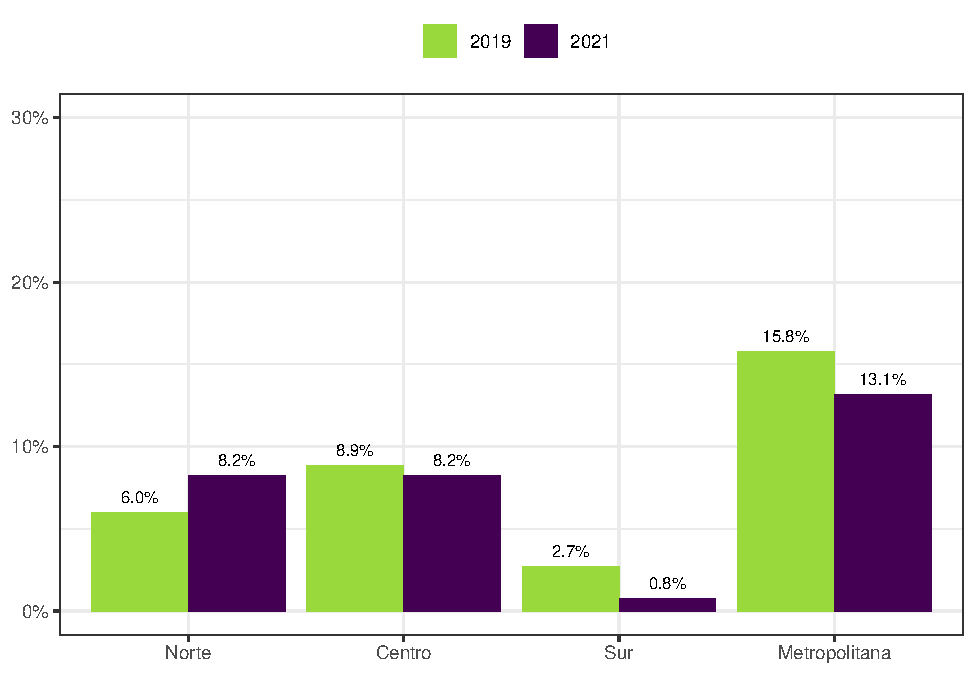
\includegraphics{reporte-elsoc_files/figure-latex/confli-zona-1} 

}

\caption{Porcentaje con alta frecuencia de conflictos barriales, según ola del estudio y zona geográfica. Porcentaje con conflictos barriales "Siempre" o "Muchas veces"}\label{fig:confli-zona}
\end{figure}

\begin{Shaded}
\begin{Highlighting}[]
\NormalTok{datos.}\FloatTok{8.4} \OtherTok{\textless{}{-}}\NormalTok{ elsoc\_long\_2016\_2021 }\SpecialCharTok{\%\textgreater{}\%} 
  \FunctionTok{filter}\NormalTok{(tipo\_atricion }\SpecialCharTok{==} \DecValTok{1} \SpecialCharTok{\&}\NormalTok{ muestra }\SpecialCharTok{==} \DecValTok{1} \SpecialCharTok{\&}\NormalTok{ ola }\SpecialCharTok{\%in\%} \FunctionTok{c}\NormalTok{(}\DecValTok{4}\NormalTok{,}\DecValTok{5}\NormalTok{) }\SpecialCharTok{\&} \SpecialCharTok{!}\NormalTok{t11\_01 }\SpecialCharTok{\%in\%} \FunctionTok{c}\NormalTok{(}\SpecialCharTok{{-}}\DecValTok{888}\NormalTok{, }\SpecialCharTok{{-}}\DecValTok{999}\NormalTok{) }\SpecialCharTok{\&}
           \SpecialCharTok{!}\NormalTok{t11\_02 }\SpecialCharTok{\%in\%} \FunctionTok{c}\NormalTok{(}\SpecialCharTok{{-}}\DecValTok{888}\NormalTok{, }\SpecialCharTok{{-}}\DecValTok{999}\NormalTok{) }\SpecialCharTok{\&} \SpecialCharTok{!}\NormalTok{t11\_03 }\SpecialCharTok{\%in\%} \FunctionTok{c}\NormalTok{(}\SpecialCharTok{{-}}\DecValTok{888}\NormalTok{, }\SpecialCharTok{{-}}\DecValTok{999}\NormalTok{) }\SpecialCharTok{\&} \SpecialCharTok{!}\NormalTok{t11\_04 }\SpecialCharTok{\%in\%} \FunctionTok{c}\NormalTok{(}\SpecialCharTok{{-}}\DecValTok{888}\NormalTok{, }\SpecialCharTok{{-}}\DecValTok{999}\NormalTok{)) }\SpecialCharTok{\%\textgreater{}\%} 
  \FunctionTok{mutate}\NormalTok{(}\AttributeTok{barrio\_confli =}\NormalTok{ (t11\_01 }\SpecialCharTok{+}\NormalTok{ t11\_02 }\SpecialCharTok{+}\NormalTok{ t11\_03 }\SpecialCharTok{+}\NormalTok{ t11\_04)}\SpecialCharTok{/}\DecValTok{4}\NormalTok{) }\SpecialCharTok{\%\textgreater{}\%}
  \FunctionTok{mutate}\NormalTok{(}\AttributeTok{barrio\_confli\_rec =} \FunctionTok{factor}\NormalTok{(}\FunctionTok{cut}\NormalTok{(barrio\_confli, }\AttributeTok{breaks =} \FunctionTok{c}\NormalTok{(}\DecValTok{0}\NormalTok{,}\DecValTok{1}\NormalTok{,}\FloatTok{2.75}\NormalTok{,}\DecValTok{5}\NormalTok{)),}
         \AttributeTok{labels =} \FunctionTok{c}\NormalTok{(}\StringTok{"Nunca"}\NormalTok{,}\StringTok{"Pocas o algunas veces"}\NormalTok{,}\StringTok{"Muchas veces o siempre"}\NormalTok{)),}
         \AttributeTok{estrato =} \FunctionTok{factor}\NormalTok{(estrato, }\AttributeTok{levels =} \FunctionTok{c}\NormalTok{(}\DecValTok{1}\NormalTok{,}\DecValTok{2}\NormalTok{,}\DecValTok{3}\NormalTok{,}\DecValTok{4}\NormalTok{,}\DecValTok{5}\NormalTok{,}\DecValTok{6}\NormalTok{),}
         \AttributeTok{labels =} \FunctionTok{c}\NormalTok{(}\StringTok{\textquotesingle{}Gran}\SpecialCharTok{\textbackslash{}n}\StringTok{Santiago\textquotesingle{}}\NormalTok{, }\StringTok{\textquotesingle{}Gran}\SpecialCharTok{\textbackslash{}n}\StringTok{Valparaíso\textquotesingle{}}\NormalTok{, }\StringTok{\textquotesingle{}Gran}\SpecialCharTok{\textbackslash{}n}\StringTok{Concepción\textquotesingle{}}\NormalTok{, }
                    \StringTok{\textquotesingle{}Ciudades}\SpecialCharTok{\textbackslash{}n}\StringTok{grandes\textquotesingle{}}\NormalTok{, }\StringTok{\textquotesingle{}Ciudades}\SpecialCharTok{\textbackslash{}n}\StringTok{medianas\textquotesingle{}}\NormalTok{, }\StringTok{\textquotesingle{}Ciudades}\SpecialCharTok{\textbackslash{}n}\StringTok{pequeñas\textquotesingle{}}\NormalTok{))) }\SpecialCharTok{\%\textgreater{}\%}
\NormalTok{  sjlabelled}\SpecialCharTok{::}\FunctionTok{as\_label}\NormalTok{(ola) }\SpecialCharTok{\%\textgreater{}\%} 
  \FunctionTok{prop}\NormalTok{(}\AttributeTok{x =}\NormalTok{ barrio\_confli\_rec, }\AttributeTok{by =} \FunctionTok{c}\NormalTok{(ola, estrato), }\AttributeTok{na.rm =} \ConstantTok{TRUE}\NormalTok{) }\SpecialCharTok{\%\textgreater{}\%} 
  \FunctionTok{filter}\NormalTok{(barrio\_confli\_rec }\SpecialCharTok{==} \StringTok{\textquotesingle{}Muchas veces o siempre\textquotesingle{}}\NormalTok{)}

\NormalTok{g8}\FloatTok{.4} \OtherTok{\textless{}{-}}\NormalTok{ datos.}\FloatTok{8.4} \SpecialCharTok{\%\textgreater{}\%} 
  \FunctionTok{ggplot}\NormalTok{(}\FunctionTok{aes}\NormalTok{(}\AttributeTok{y =}\NormalTok{ prop, }\AttributeTok{x =}\NormalTok{ estrato, }\AttributeTok{fill =}\NormalTok{ ola, }
             \AttributeTok{label =} \FunctionTok{as.character}\NormalTok{(scales}\SpecialCharTok{::}\FunctionTok{percent}\NormalTok{(prop, }\AttributeTok{accuracy =}\NormalTok{ .}\DecValTok{1}\NormalTok{)))) }\SpecialCharTok{+} 
  \FunctionTok{theme\_bw}\NormalTok{() }\SpecialCharTok{+} 
  \FunctionTok{geom\_col}\NormalTok{(}\AttributeTok{position =} \StringTok{\textquotesingle{}Dodge\textquotesingle{}}\NormalTok{) }\SpecialCharTok{+}
  \FunctionTok{scale\_y\_continuous}\NormalTok{(}\AttributeTok{labels =}\NormalTok{ scales}\SpecialCharTok{::}\NormalTok{percent,}
                     \AttributeTok{limits =} \FunctionTok{c}\NormalTok{(}\DecValTok{0}\NormalTok{, .}\DecValTok{3}\NormalTok{)) }\SpecialCharTok{+}
  \FunctionTok{ylab}\NormalTok{(}\AttributeTok{label =} \ConstantTok{NULL}\NormalTok{) }\SpecialCharTok{+}
  \FunctionTok{xlab}\NormalTok{(}\AttributeTok{label =} \ConstantTok{NULL}\NormalTok{) }\SpecialCharTok{+}
  \FunctionTok{scale\_fill\_viridis\_d}\NormalTok{(}\AttributeTok{begin =} \DecValTok{0}\NormalTok{, }\AttributeTok{end =}\NormalTok{ .}\DecValTok{85}\NormalTok{, }\AttributeTok{direction =} \SpecialCharTok{{-}}\DecValTok{1}\NormalTok{, }\AttributeTok{option =} \StringTok{\textquotesingle{}viridis\textquotesingle{}}\NormalTok{) }\SpecialCharTok{+}
  \FunctionTok{theme}\NormalTok{(}\AttributeTok{legend.position =} \StringTok{\textquotesingle{}top\textquotesingle{}}\NormalTok{,}
        \AttributeTok{legend.title =} \FunctionTok{element\_blank}\NormalTok{()) }\SpecialCharTok{+}
  \FunctionTok{geom\_text}\NormalTok{(}\AttributeTok{vjust =} \SpecialCharTok{{-}}\FloatTok{0.8}\NormalTok{,}
            \AttributeTok{position =} \FunctionTok{position\_dodge}\NormalTok{(}\AttributeTok{width =}\NormalTok{ .}\DecValTok{9}\NormalTok{),}
            \AttributeTok{size=} \FloatTok{2.75}\NormalTok{)}
\NormalTok{g8}\FloatTok{.4}
\end{Highlighting}
\end{Shaded}

\begin{figure}

{\centering 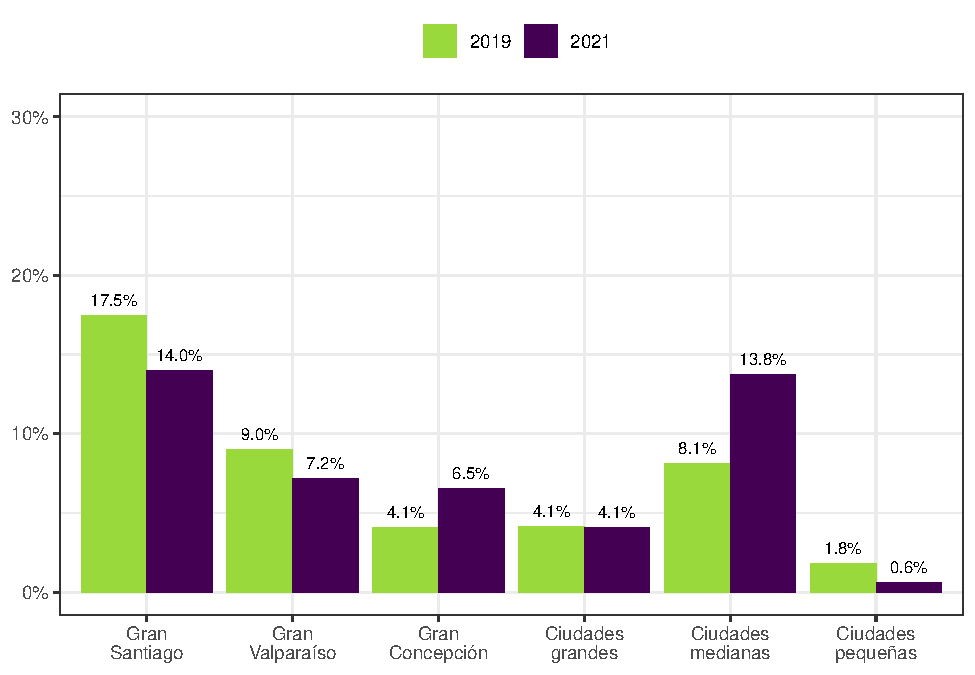
\includegraphics{reporte-elsoc_files/figure-latex/confli-estrato-1} 

}

\caption{Porcentaje con alta frecuencia de conflictos barriales, según ola del estudio y zona de residencia. Porcentaje con conflictos barriales "Siempre" o "Muchas veces".}\label{fig:confli-estrato}
\end{figure}

\begin{Shaded}
\begin{Highlighting}[]
\NormalTok{datos.}\FloatTok{8.5} \OtherTok{\textless{}{-}}\NormalTok{ elsoc\_long\_2016\_2021 }\SpecialCharTok{\%\textgreater{}\%} 
  \FunctionTok{filter}\NormalTok{(tipo\_atricion }\SpecialCharTok{==} \DecValTok{1} \SpecialCharTok{\&}\NormalTok{ muestra }\SpecialCharTok{==} \DecValTok{1} \SpecialCharTok{\&}\NormalTok{ ola }\SpecialCharTok{\%in\%} \FunctionTok{c}\NormalTok{(}\DecValTok{4}\NormalTok{,}\DecValTok{5}\NormalTok{) }\SpecialCharTok{\&} \SpecialCharTok{!}\NormalTok{t11\_01 }\SpecialCharTok{\%in\%} \FunctionTok{c}\NormalTok{(}\SpecialCharTok{{-}}\DecValTok{888}\NormalTok{, }\SpecialCharTok{{-}}\DecValTok{999}\NormalTok{) }\SpecialCharTok{\&}
           \SpecialCharTok{!}\NormalTok{t11\_02 }\SpecialCharTok{\%in\%} \FunctionTok{c}\NormalTok{(}\SpecialCharTok{{-}}\DecValTok{888}\NormalTok{, }\SpecialCharTok{{-}}\DecValTok{999}\NormalTok{) }\SpecialCharTok{\&} \SpecialCharTok{!}\NormalTok{t11\_03 }\SpecialCharTok{\%in\%} \FunctionTok{c}\NormalTok{(}\SpecialCharTok{{-}}\DecValTok{888}\NormalTok{, }\SpecialCharTok{{-}}\DecValTok{999}\NormalTok{) }\SpecialCharTok{\&} \SpecialCharTok{!}\NormalTok{t11\_04 }\SpecialCharTok{\%in\%} \FunctionTok{c}\NormalTok{(}\SpecialCharTok{{-}}\DecValTok{888}\NormalTok{, }\SpecialCharTok{{-}}\DecValTok{999}\NormalTok{)) }\SpecialCharTok{\%\textgreater{}\%} 
  \FunctionTok{mutate}\NormalTok{(}\AttributeTok{barrio\_confli =}\NormalTok{ (t11\_01 }\SpecialCharTok{+}\NormalTok{ t11\_02 }\SpecialCharTok{+}\NormalTok{ t11\_03 }\SpecialCharTok{+}\NormalTok{ t11\_04)}\SpecialCharTok{/}\DecValTok{4}\NormalTok{,}
         \AttributeTok{m30 =} \FunctionTok{as.numeric}\NormalTok{(car}\SpecialCharTok{::}\FunctionTok{recode}\NormalTok{(m30,}\StringTok{"1=110000;2=251000;3=305000;4=355000;5=400000;}
\StringTok{                                           6=445000;7=490000;8=535000;9=585000;10=640000;11=700000;12=765000;}
\StringTok{                                           13=845000;14=935000;15=1040000;16=1180000;17=1375000;18=1670000;}
\StringTok{                                           19=2275000;20=2700000;NA=NA"}\NormalTok{)),}
         \AttributeTok{m29\_imp =} \FunctionTok{ifelse}\NormalTok{(}\SpecialCharTok{!}\FunctionTok{is.na}\NormalTok{(m29),m29, m30),}
         \AttributeTok{n\_hogar =} \FunctionTok{case\_when}\NormalTok{(ola }\SpecialCharTok{==} \DecValTok{1} \SpecialCharTok{\textasciitilde{}}\NormalTok{ nhogar1, ola }\SpecialCharTok{==} \DecValTok{2} \SpecialCharTok{\textasciitilde{}}\NormalTok{ m46\_nhogar,}
\NormalTok{                             ola }\SpecialCharTok{==} \DecValTok{3} \SpecialCharTok{\textasciitilde{}}\NormalTok{ m54, ola }\SpecialCharTok{==} \DecValTok{4} \SpecialCharTok{\textasciitilde{}}\NormalTok{ m54, ola }\SpecialCharTok{==} \DecValTok{5} \SpecialCharTok{\textasciitilde{}}\NormalTok{ m54)) }\SpecialCharTok{\%\textgreater{}\%}
  \FunctionTok{mutate}\NormalTok{(}\AttributeTok{ing\_pc =}\NormalTok{ (m29\_imp}\SpecialCharTok{/}\NormalTok{n\_hogar)) }\SpecialCharTok{\%\textgreater{}\%}
\NormalTok{  sjlabelled}\SpecialCharTok{::}\FunctionTok{as\_label}\NormalTok{(ola) }\SpecialCharTok{\%\textgreater{}\%} 
  \FunctionTok{group\_by}\NormalTok{(ola) }\SpecialCharTok{\%\textgreater{}\%} 
  \FunctionTok{mutate}\NormalTok{(}\AttributeTok{quintil =} \FunctionTok{factor}\NormalTok{(}\FunctionTok{ntile}\NormalTok{(}\SpecialCharTok{{-}}\FunctionTok{desc}\NormalTok{(ing\_pc), }\DecValTok{5}\NormalTok{), }\AttributeTok{levels =} \FunctionTok{c}\NormalTok{(}\DecValTok{1}\NormalTok{,}\DecValTok{2}\NormalTok{,}\DecValTok{3}\NormalTok{,}\DecValTok{4}\NormalTok{,}\DecValTok{5}\NormalTok{),}
         \AttributeTok{labels =} \FunctionTok{c}\NormalTok{(}\StringTok{\textquotesingle{}Q1\textquotesingle{}}\NormalTok{, }\StringTok{\textquotesingle{}Q2\textquotesingle{}}\NormalTok{, }\StringTok{\textquotesingle{}Q3\textquotesingle{}}\NormalTok{, }\StringTok{\textquotesingle{}Q4\textquotesingle{}}\NormalTok{, }\StringTok{\textquotesingle{}Q5\textquotesingle{}}\NormalTok{))) }\SpecialCharTok{\%\textgreater{}\%} 
  \FunctionTok{prop}\NormalTok{(}\AttributeTok{x =}\NormalTok{ barrio\_confli }\SpecialCharTok{\textgreater{}=} \FloatTok{2.76}\NormalTok{, }\AttributeTok{by =} \FunctionTok{c}\NormalTok{(ola, quintil), }\AttributeTok{na.rm =} \ConstantTok{TRUE}\NormalTok{)}

\NormalTok{g8}\FloatTok{.5} \OtherTok{\textless{}{-}}\NormalTok{ datos.}\FloatTok{8.5} \SpecialCharTok{\%\textgreater{}\%} 
  \FunctionTok{ggplot}\NormalTok{(}\FunctionTok{aes}\NormalTok{(}\AttributeTok{y =}\NormalTok{ prop, }\AttributeTok{x =}\NormalTok{ quintil, }\AttributeTok{fill =}\NormalTok{ ola, }
             \AttributeTok{label =} \FunctionTok{as.character}\NormalTok{(scales}\SpecialCharTok{::}\FunctionTok{percent}\NormalTok{(prop, }\AttributeTok{accuracy =}\NormalTok{ .}\DecValTok{1}\NormalTok{)))) }\SpecialCharTok{+} 
  \FunctionTok{theme\_bw}\NormalTok{() }\SpecialCharTok{+} 
  \FunctionTok{geom\_col}\NormalTok{(}\AttributeTok{position =} \StringTok{\textquotesingle{}Dodge\textquotesingle{}}\NormalTok{) }\SpecialCharTok{+}
  \FunctionTok{scale\_y\_continuous}\NormalTok{(}\AttributeTok{labels =}\NormalTok{ scales}\SpecialCharTok{::}\NormalTok{percent,}
                     \AttributeTok{limits =} \FunctionTok{c}\NormalTok{(}\DecValTok{0}\NormalTok{, .}\DecValTok{3}\NormalTok{)) }\SpecialCharTok{+}
  \FunctionTok{ylab}\NormalTok{(}\AttributeTok{label =} \ConstantTok{NULL}\NormalTok{) }\SpecialCharTok{+}
  \FunctionTok{xlab}\NormalTok{(}\AttributeTok{label =} \ConstantTok{NULL}\NormalTok{) }\SpecialCharTok{+}
  \FunctionTok{scale\_fill\_viridis\_d}\NormalTok{(}\AttributeTok{begin =} \DecValTok{0}\NormalTok{, }\AttributeTok{end =}\NormalTok{ .}\DecValTok{85}\NormalTok{, }\AttributeTok{direction =} \SpecialCharTok{{-}}\DecValTok{1}\NormalTok{, }\AttributeTok{option =} \StringTok{\textquotesingle{}viridis\textquotesingle{}}\NormalTok{) }\SpecialCharTok{+}
  \FunctionTok{theme}\NormalTok{(}\AttributeTok{legend.position =} \StringTok{\textquotesingle{}top\textquotesingle{}}\NormalTok{,}
        \AttributeTok{legend.title =} \FunctionTok{element\_blank}\NormalTok{()) }\SpecialCharTok{+}
  \FunctionTok{geom\_text}\NormalTok{(}\AttributeTok{vjust =} \SpecialCharTok{{-}}\FloatTok{0.8}\NormalTok{,}
            \AttributeTok{position =} \FunctionTok{position\_dodge}\NormalTok{(}\AttributeTok{width =}\NormalTok{ .}\DecValTok{9}\NormalTok{),}
            \AttributeTok{size=} \FloatTok{2.75}\NormalTok{)}
\NormalTok{g8}\FloatTok{.5}
\end{Highlighting}
\end{Shaded}

\begin{figure}

{\centering 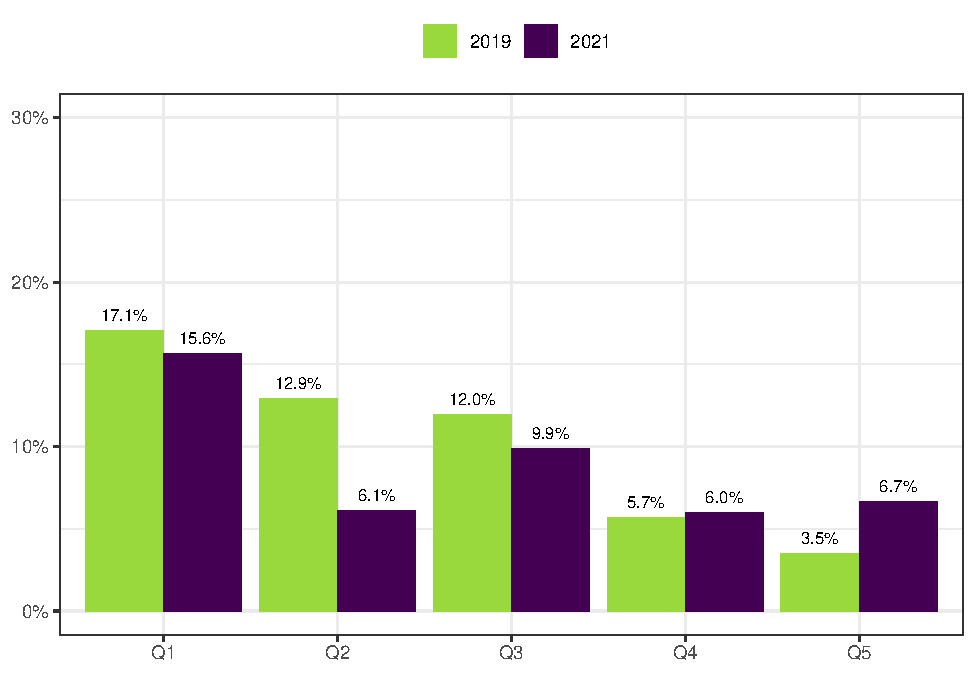
\includegraphics{reporte-elsoc_files/figure-latex/confli-quintil-1} 

}

\caption{Porcentaje con alta frecuencia de conflictos barriales, según ola del estudio y quintil de ingreso. Porcentaje con conflictos barriales "Siempre" o "Muchas veces".}\label{fig:confli-quintil}
\end{figure}

\hypertarget{cartografuxeda-del-conflicto-barrial}{%
\subsection{Cartografía del conflicto barrial}\label{cartografuxeda-del-conflicto-barrial}}

\begin{Shaded}
\begin{Highlighting}[]
\NormalTok{elsoc\_comuna\_rm }\OtherTok{\textless{}{-}}\NormalTok{ elsoc\_long\_2016\_2021 }\SpecialCharTok{\%\textgreater{}\%} 
  \FunctionTok{filter}\NormalTok{(tipo\_atricion }\SpecialCharTok{==} \DecValTok{1} \SpecialCharTok{\&}\NormalTok{ muestra }\SpecialCharTok{==} \DecValTok{1} \SpecialCharTok{\&}\NormalTok{ ola }\SpecialCharTok{==} \DecValTok{5} \SpecialCharTok{\&}\NormalTok{ region\_cod }\SpecialCharTok{==} \DecValTok{13} \SpecialCharTok{\&} \SpecialCharTok{!}\NormalTok{t11\_01 }\SpecialCharTok{\%in\%} \FunctionTok{c}\NormalTok{(}\SpecialCharTok{{-}}\DecValTok{888}\NormalTok{, }\SpecialCharTok{{-}}\DecValTok{999}\NormalTok{) }\SpecialCharTok{\&}
           \SpecialCharTok{!}\NormalTok{t11\_02 }\SpecialCharTok{\%in\%} \FunctionTok{c}\NormalTok{(}\SpecialCharTok{{-}}\DecValTok{888}\NormalTok{, }\SpecialCharTok{{-}}\DecValTok{999}\NormalTok{) }\SpecialCharTok{\&} \SpecialCharTok{!}\NormalTok{t11\_03 }\SpecialCharTok{\%in\%} \FunctionTok{c}\NormalTok{(}\SpecialCharTok{{-}}\DecValTok{888}\NormalTok{, }\SpecialCharTok{{-}}\DecValTok{999}\NormalTok{) }\SpecialCharTok{\&} \SpecialCharTok{!}\NormalTok{t11\_04 }\SpecialCharTok{\%in\%} \FunctionTok{c}\NormalTok{(}\SpecialCharTok{{-}}\DecValTok{888}\NormalTok{, }\SpecialCharTok{{-}}\DecValTok{999}\NormalTok{)) }\SpecialCharTok{\%\textgreater{}\%} 
  \FunctionTok{mutate}\NormalTok{(}\AttributeTok{barrio\_confli =}\NormalTok{ (t11\_01 }\SpecialCharTok{+}\NormalTok{ t11\_02 }\SpecialCharTok{+}\NormalTok{ t11\_03 }\SpecialCharTok{+}\NormalTok{ t11\_04)}\SpecialCharTok{/}\DecValTok{4}\NormalTok{) }\SpecialCharTok{\%\textgreater{}\%}
\NormalTok{  sjlabelled}\SpecialCharTok{::}\FunctionTok{as\_label}\NormalTok{(ola) }\SpecialCharTok{\%\textgreater{}\%} 
  \FunctionTok{group\_by}\NormalTok{(comuna, comuna\_cod) }\SpecialCharTok{\%\textgreater{}\%} 
  \FunctionTok{summarise}\NormalTok{(}\AttributeTok{m\_confli =} \FunctionTok{weighted.mean}\NormalTok{(barrio\_confli, ponderador02, }\AttributeTok{na.rm =}\NormalTok{ T)) }\SpecialCharTok{\%\textgreater{}\%} 
  \FunctionTok{ungroup}\NormalTok{() }

\NormalTok{comunas\_rm }\OtherTok{\textless{}{-}}\NormalTok{ chilemapas}\SpecialCharTok{::}\NormalTok{mapa\_zonas }\SpecialCharTok{\%\textgreater{}\%}   
\NormalTok{  dplyr}\SpecialCharTok{::}\FunctionTok{filter}\NormalTok{(codigo\_region }\SpecialCharTok{==} \StringTok{\textquotesingle{}13\textquotesingle{}} \SpecialCharTok{\&}\NormalTok{ codigo\_provincia }\SpecialCharTok{==} \StringTok{\textquotesingle{}131\textquotesingle{}}\NormalTok{) }\SpecialCharTok{\%\textgreater{}\%} 
  \FunctionTok{st\_as\_sf}\NormalTok{(.) }\SpecialCharTok{\%\textgreater{}\%} 
  \FunctionTok{group\_by}\NormalTok{(codigo\_comuna) }\SpecialCharTok{\%\textgreater{}\%} 
  \FunctionTok{summarise}\NormalTok{() }\SpecialCharTok{\%\textgreater{}\%} 
  \FunctionTok{ungroup}\NormalTok{() }\SpecialCharTok{\%\textgreater{}\%} 
  \FunctionTok{mutate}\NormalTok{(}\AttributeTok{comuna\_cod =} \FunctionTok{as.numeric}\NormalTok{(codigo\_comuna)) }\SpecialCharTok{\%\textgreater{}\%} 
  \FunctionTok{left\_join}\NormalTok{(elsoc\_comuna\_rm, }\AttributeTok{by =} \StringTok{\textquotesingle{}comuna\_cod\textquotesingle{}}\NormalTok{)}

\NormalTok{g.confli.rm }\OtherTok{\textless{}{-}}\NormalTok{ comunas\_rm }\SpecialCharTok{\%\textgreater{}\%}
  \FunctionTok{ggplot}\NormalTok{() }\SpecialCharTok{+} 
  \FunctionTok{geom\_sf}\NormalTok{(}\FunctionTok{aes}\NormalTok{(}\AttributeTok{fill =}\NormalTok{ m\_confli, }\AttributeTok{geometry =}\NormalTok{ geometry)) }\SpecialCharTok{+}
  \FunctionTok{labs}\NormalTok{(}\AttributeTok{y =} \ConstantTok{NULL}\NormalTok{, }\AttributeTok{x =} \ConstantTok{NULL}\NormalTok{, }\AttributeTok{fill =} \StringTok{"Conflictividad barrial}\SpecialCharTok{\textbackslash{}n}\StringTok{promedio por comuna"}\NormalTok{) }\SpecialCharTok{+}
  \FunctionTok{scale\_fill\_viridis\_c}\NormalTok{(}\AttributeTok{begin =}\NormalTok{ .}\DecValTok{11}\NormalTok{, }\AttributeTok{end =}\NormalTok{ .}\DecValTok{88}\NormalTok{, }\AttributeTok{direction =} \SpecialCharTok{{-}}\DecValTok{1}\NormalTok{, }\AttributeTok{option =} \StringTok{\textquotesingle{}viridis\textquotesingle{}}\NormalTok{) }\SpecialCharTok{+}
  \FunctionTok{theme\_bw}\NormalTok{()}
\NormalTok{g.confli.rm}
\end{Highlighting}
\end{Shaded}

\begin{figure}

{\centering 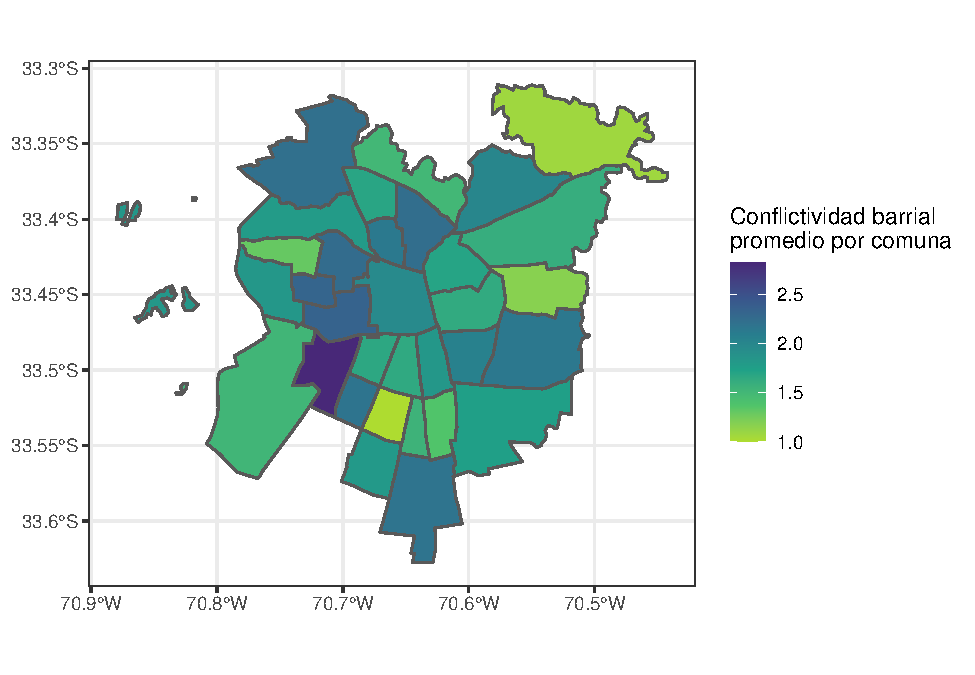
\includegraphics{reporte-elsoc_files/figure-latex/confli-comuna-1} 

}

\caption{Frecuencia promedio de problemas con vecinos, según comuna de residencia en la región metropolitana (2021).}\label{fig:confli-comuna}
\end{figure}

\begin{Shaded}
\begin{Highlighting}[]
\NormalTok{elsoc\_region }\OtherTok{\textless{}{-}}\NormalTok{ elsoc\_long\_2016\_2021 }\SpecialCharTok{\%\textgreater{}\%} 
  \FunctionTok{filter}\NormalTok{(tipo\_atricion }\SpecialCharTok{==} \DecValTok{1} \SpecialCharTok{\&}\NormalTok{ muestra }\SpecialCharTok{==} \DecValTok{1} \SpecialCharTok{\&}\NormalTok{ ola }\SpecialCharTok{==} \DecValTok{5} \SpecialCharTok{\&} \SpecialCharTok{!}\NormalTok{t11\_01 }\SpecialCharTok{\%in\%} \FunctionTok{c}\NormalTok{(}\SpecialCharTok{{-}}\DecValTok{888}\NormalTok{, }\SpecialCharTok{{-}}\DecValTok{999}\NormalTok{) }\SpecialCharTok{\&}
           \SpecialCharTok{!}\NormalTok{t11\_02 }\SpecialCharTok{\%in\%} \FunctionTok{c}\NormalTok{(}\SpecialCharTok{{-}}\DecValTok{888}\NormalTok{, }\SpecialCharTok{{-}}\DecValTok{999}\NormalTok{) }\SpecialCharTok{\&} \SpecialCharTok{!}\NormalTok{t11\_03 }\SpecialCharTok{\%in\%} \FunctionTok{c}\NormalTok{(}\SpecialCharTok{{-}}\DecValTok{888}\NormalTok{, }\SpecialCharTok{{-}}\DecValTok{999}\NormalTok{) }\SpecialCharTok{\&} \SpecialCharTok{!}\NormalTok{t11\_04 }\SpecialCharTok{\%in\%} \FunctionTok{c}\NormalTok{(}\SpecialCharTok{{-}}\DecValTok{888}\NormalTok{, }\SpecialCharTok{{-}}\DecValTok{999}\NormalTok{)) }\SpecialCharTok{\%\textgreater{}\%} 
  \FunctionTok{mutate}\NormalTok{(}\AttributeTok{barrio\_confli =}\NormalTok{ (t11\_01 }\SpecialCharTok{+}\NormalTok{ t11\_02 }\SpecialCharTok{+}\NormalTok{ t11\_03 }\SpecialCharTok{+}\NormalTok{ t11\_04)}\SpecialCharTok{/}\DecValTok{4}\NormalTok{) }\SpecialCharTok{\%\textgreater{}\%}
\NormalTok{  sjlabelled}\SpecialCharTok{::}\FunctionTok{as\_label}\NormalTok{(ola) }\SpecialCharTok{\%\textgreater{}\%} 
  \FunctionTok{group\_by}\NormalTok{(region, region\_cod) }\SpecialCharTok{\%\textgreater{}\%} 
  \FunctionTok{summarise}\NormalTok{(}\AttributeTok{m\_confli =} \FunctionTok{weighted.mean}\NormalTok{(barrio\_confli, ponderador02, }\AttributeTok{na.rm =}\NormalTok{ T),}
            \AttributeTok{sd\_confli =} \FunctionTok{sd}\NormalTok{(barrio\_confli, }\AttributeTok{na.rm =}\NormalTok{ T),}
            \AttributeTok{n =} \FunctionTok{n}\NormalTok{())}

\NormalTok{elsoc\_region}\SpecialCharTok{$}\NormalTok{region\_cod }\OtherTok{\textless{}{-}} \FunctionTok{factor}\NormalTok{(elsoc\_region}\SpecialCharTok{$}\NormalTok{region\_cod,}
                                  \AttributeTok{labels =} \FunctionTok{c}\NormalTok{(}\StringTok{\textquotesingle{}01\textquotesingle{}}\NormalTok{,}\StringTok{\textquotesingle{}02\textquotesingle{}}\NormalTok{,}\StringTok{\textquotesingle{}03\textquotesingle{}}\NormalTok{,}\StringTok{\textquotesingle{}04\textquotesingle{}}\NormalTok{,}\StringTok{\textquotesingle{}05\textquotesingle{}}\NormalTok{,}\StringTok{\textquotesingle{}06\textquotesingle{}}\NormalTok{,}\StringTok{\textquotesingle{}07\textquotesingle{}}\NormalTok{,}\StringTok{\textquotesingle{}08\textquotesingle{}}\NormalTok{,}
                                            \StringTok{\textquotesingle{}09\textquotesingle{}}\NormalTok{,}\StringTok{\textquotesingle{}10\textquotesingle{}}\NormalTok{,}\StringTok{\textquotesingle{}11\textquotesingle{}}\NormalTok{,}\StringTok{\textquotesingle{}13\textquotesingle{}}\NormalTok{,}\StringTok{\textquotesingle{}14\textquotesingle{}}\NormalTok{,}\StringTok{\textquotesingle{}15\textquotesingle{}}\NormalTok{,}\StringTok{\textquotesingle{}16\textquotesingle{}}\NormalTok{))}

\NormalTok{regiones }\OtherTok{\textless{}{-}}\NormalTok{ chilemapas}\SpecialCharTok{::}\FunctionTok{generar\_regiones}\NormalTok{()}
\NormalTok{regiones }\OtherTok{\textless{}{-}} \FunctionTok{merge}\NormalTok{(regiones,elsoc\_region, }\AttributeTok{by.x=}\StringTok{"codigo\_region"}\NormalTok{,}\AttributeTok{by.y=}\StringTok{"region\_cod"}\NormalTok{,}\AttributeTok{all.x=}\ConstantTok{TRUE}\NormalTok{,}\AttributeTok{sort=}\NormalTok{F)}

\CommentTok{\#para intentar hacer facet\_wrap}
\CommentTok{\#regiones$mitad \textless{}{-} c(\textquotesingle{}1\textquotesingle{},\textquotesingle{}1\textquotesingle{},\textquotesingle{}1\textquotesingle{},\textquotesingle{}1\textquotesingle{},\textquotesingle{}1\textquotesingle{},\textquotesingle{}1\textquotesingle{},\textquotesingle{}1\textquotesingle{},\textquotesingle{}2\textquotesingle{},\textquotesingle{}2\textquotesingle{},\textquotesingle{}2\textquotesingle{},\textquotesingle{}2\textquotesingle{},\textquotesingle{}1\textquotesingle{},\textquotesingle{}2\textquotesingle{},\textquotesingle{}1\textquotesingle{},\textquotesingle{}2\textquotesingle{},\textquotesingle{}2\textquotesingle{})}

\NormalTok{regiones}\SpecialCharTok{$}\NormalTok{region[}\FunctionTok{is.na}\NormalTok{(regiones}\SpecialCharTok{$}\NormalTok{region)] }\OtherTok{\textless{}{-}} \StringTok{\textquotesingle{}Magallanes}\SpecialCharTok{\textbackslash{}n}\StringTok{(Sin datos)\textquotesingle{}}
\NormalTok{regiones}\SpecialCharTok{$}\NormalTok{region[regiones}\SpecialCharTok{$}\NormalTok{region }\SpecialCharTok{==} \StringTok{\textquotesingle{}Metropolitana de santiago\textquotesingle{}}\NormalTok{] }\OtherTok{\textless{}{-}} \StringTok{\textquotesingle{}Metropolitana\textquotesingle{}}
\NormalTok{regiones}\SpecialCharTok{$}\NormalTok{region[regiones}\SpecialCharTok{$}\NormalTok{region }\SpecialCharTok{==} \StringTok{\textquotesingle{}Libertador general bernardo ohiggins\textquotesingle{}}\NormalTok{] }\OtherTok{\textless{}{-}} \StringTok{\textquotesingle{}Ohiggins\textquotesingle{}}
\NormalTok{regiones}\SpecialCharTok{$}\NormalTok{region[regiones}\SpecialCharTok{$}\NormalTok{region }\SpecialCharTok{==} \StringTok{\textquotesingle{}Aysen del general carlos ibannez del campo\textquotesingle{}}\NormalTok{] }\OtherTok{\textless{}{-}} \StringTok{\textquotesingle{}Aysen\textquotesingle{}}
\NormalTok{regiones}\SpecialCharTok{$}\NormalTok{region[regiones}\SpecialCharTok{$}\NormalTok{region }\SpecialCharTok{==} \StringTok{\textquotesingle{}Arica y parinacota\textquotesingle{}}\NormalTok{] }\OtherTok{\textless{}{-}} \StringTok{\textquotesingle{}Arica\textquotesingle{}}

\NormalTok{g.confli.region }\OtherTok{\textless{}{-}}\NormalTok{ regiones }\SpecialCharTok{\%\textgreater{}\%} 
  \FunctionTok{ggplot}\NormalTok{(}\FunctionTok{aes}\NormalTok{(}\AttributeTok{fill =}\NormalTok{ m\_confli, }\AttributeTok{geometry =}\NormalTok{ geometry, }\AttributeTok{label =}\NormalTok{ region)) }\SpecialCharTok{+} 
  \FunctionTok{geom\_sf}\NormalTok{() }\SpecialCharTok{+}
  \FunctionTok{coord\_sf}\NormalTok{(}\AttributeTok{xlim =} \FunctionTok{c}\NormalTok{(}\SpecialCharTok{{-}}\DecValTok{100}\NormalTok{, }\SpecialCharTok{{-}}\DecValTok{65}\NormalTok{)) }\SpecialCharTok{+}
  \FunctionTok{labs}\NormalTok{(}\AttributeTok{y =} \ConstantTok{NULL}\NormalTok{, }\AttributeTok{x =} \ConstantTok{NULL}\NormalTok{, }\AttributeTok{fill =} \StringTok{"Conflictividad barrial}\SpecialCharTok{\textbackslash{}n}\StringTok{promedio por región"}\NormalTok{) }\SpecialCharTok{+}
  \FunctionTok{scale\_fill\_viridis\_c}\NormalTok{(}\AttributeTok{begin =}\NormalTok{ .}\DecValTok{11}\NormalTok{, }\AttributeTok{end =}\NormalTok{ .}\DecValTok{88}\NormalTok{, }\AttributeTok{direction =} \SpecialCharTok{{-}}\DecValTok{1}\NormalTok{, }\AttributeTok{option =} \StringTok{\textquotesingle{}viridis\textquotesingle{}}\NormalTok{, }\AttributeTok{na.value =} \StringTok{\textquotesingle{}white\textquotesingle{}}\NormalTok{) }\SpecialCharTok{+}
\NormalTok{  ggrepel}\SpecialCharTok{::}\FunctionTok{geom\_text\_repel}\NormalTok{(}\AttributeTok{stat =} \StringTok{"sf\_coordinates"}\NormalTok{, }\AttributeTok{min.segment.length =} \DecValTok{0}\NormalTok{,}
                           \AttributeTok{colour =} \StringTok{"black"}\NormalTok{, }\AttributeTok{segment.colour =} \StringTok{"black"}\NormalTok{,}
                           \AttributeTok{direction =} \StringTok{"y"}\NormalTok{, }\AttributeTok{hjust =} \FloatTok{2.5}\NormalTok{, }\AttributeTok{size =} \DecValTok{3}\NormalTok{) }\SpecialCharTok{+}
\NormalTok{  ggspatial}\SpecialCharTok{::}\FunctionTok{annotation\_north\_arrow}\NormalTok{(}\FunctionTok{aes}\NormalTok{(}\AttributeTok{which\_north =} \StringTok{"true"}\NormalTok{, }\AttributeTok{location =} \StringTok{"bl"}\NormalTok{), }\AttributeTok{pad\_y =} \FunctionTok{unit}\NormalTok{(}\FloatTok{0.8}\NormalTok{, }\StringTok{"cm"}\NormalTok{)) }\SpecialCharTok{+}
\NormalTok{  ggspatial}\SpecialCharTok{::}\FunctionTok{annotation\_scale}\NormalTok{(}\FunctionTok{aes}\NormalTok{(}\AttributeTok{location =} \StringTok{"bl"}\NormalTok{, }\AttributeTok{style =} \StringTok{"bar"}\NormalTok{)) }\SpecialCharTok{+}
  \FunctionTok{theme\_bw}\NormalTok{()}
\NormalTok{g.confli.region}
\end{Highlighting}
\end{Shaded}

\begin{figure}

{\centering 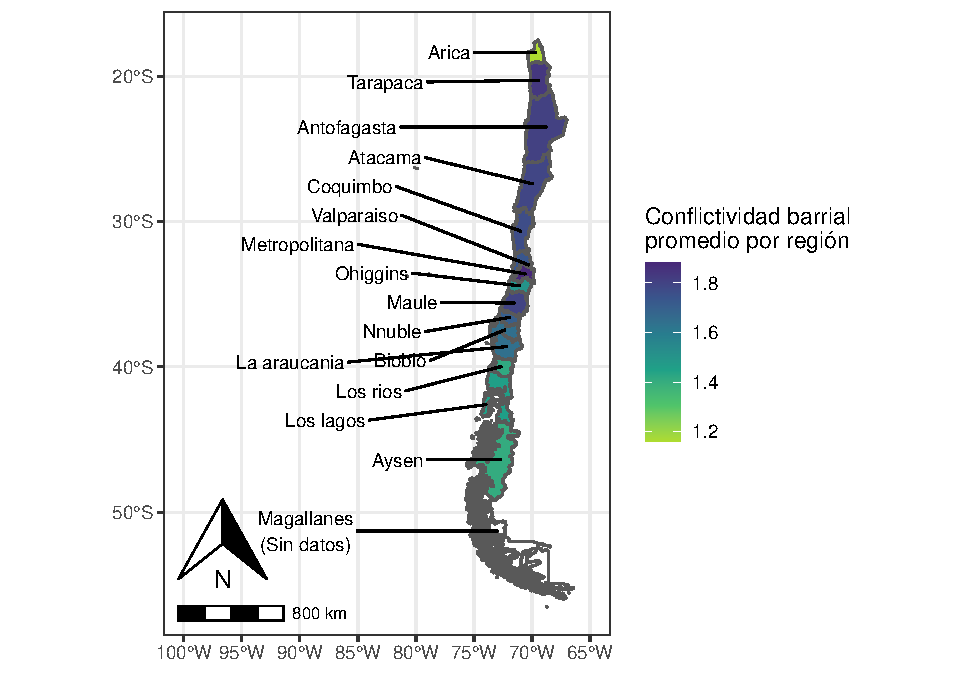
\includegraphics{reporte-elsoc_files/figure-latex/confli-region2-1} 

}

\caption{Frecuencia promedio de problemas con vecinos, según región de Chile (2021)}\label{fig:confli-region2}
\end{figure}

\hypertarget{confianza-en-vecinos}{%
\section{Confianza en vecinos}\label{confianza-en-vecinos}}

\begin{Shaded}
\begin{Highlighting}[]
\NormalTok{datos.}\FloatTok{8.6} \OtherTok{\textless{}{-}}\NormalTok{ elsoc\_long\_2016\_2021 }\SpecialCharTok{\%\textgreater{}\%} 
  \FunctionTok{filter}\NormalTok{(tipo\_atricion }\SpecialCharTok{==} \DecValTok{1} \SpecialCharTok{\&}\NormalTok{ muestra }\SpecialCharTok{==} \DecValTok{1} \SpecialCharTok{\&} \SpecialCharTok{!}\NormalTok{t01 }\SpecialCharTok{\%in\%} \FunctionTok{c}\NormalTok{(}\SpecialCharTok{{-}}\DecValTok{888}\NormalTok{, }\SpecialCharTok{{-}}\DecValTok{999}\NormalTok{)) }\SpecialCharTok{\%\textgreater{}\%} 
  \FunctionTok{mutate}\NormalTok{(}\AttributeTok{barrio\_conf =} \FunctionTok{factor}\NormalTok{(car}\SpecialCharTok{::}\FunctionTok{recode}\NormalTok{(t01, }\StringTok{"c(1,2) = 1; c(3) = 2; c(4,5) = 3"}\NormalTok{),}
                               \AttributeTok{levels =} \FunctionTok{c}\NormalTok{(}\DecValTok{1}\NormalTok{,}\DecValTok{2}\NormalTok{,}\DecValTok{3}\NormalTok{),}
                               \AttributeTok{labels =} \FunctionTok{c}\NormalTok{(}\StringTok{\textquotesingle{}Muy poco o poco\textquotesingle{}}\NormalTok{, }\StringTok{\textquotesingle{}Algo\textquotesingle{}}\NormalTok{, }\StringTok{\textquotesingle{}Bastante o mucho\textquotesingle{}}\NormalTok{))) }\SpecialCharTok{\%\textgreater{}\%}
\NormalTok{  sjlabelled}\SpecialCharTok{::}\FunctionTok{as\_label}\NormalTok{(ola) }\SpecialCharTok{\%\textgreater{}\%}
  \FunctionTok{prop}\NormalTok{(}\AttributeTok{x =}\NormalTok{ barrio\_conf, }\AttributeTok{by =}\NormalTok{ ola, }\AttributeTok{na.rm =} \ConstantTok{TRUE}\NormalTok{)}

\NormalTok{g8}\FloatTok{.6} \OtherTok{\textless{}{-}}\NormalTok{ datos.}\FloatTok{8.6} \SpecialCharTok{\%\textgreater{}\%} 
  \FunctionTok{ggplot}\NormalTok{(}\FunctionTok{aes}\NormalTok{(}\AttributeTok{y =}\NormalTok{ prop, }\AttributeTok{x =}\NormalTok{ ola, }\AttributeTok{fill =}\NormalTok{ barrio\_conf, }
             \AttributeTok{label =} \FunctionTok{as.character}\NormalTok{(scales}\SpecialCharTok{::}\FunctionTok{percent}\NormalTok{(prop, }\AttributeTok{accuracy =}\NormalTok{ .}\DecValTok{1}\NormalTok{)))) }\SpecialCharTok{+} 
  \FunctionTok{theme\_bw}\NormalTok{() }\SpecialCharTok{+} 
  \FunctionTok{geom\_col}\NormalTok{(}\AttributeTok{position =} \StringTok{\textquotesingle{}Stack\textquotesingle{}}\NormalTok{) }\SpecialCharTok{+}
  \FunctionTok{ylab}\NormalTok{(}\AttributeTok{label =} \ConstantTok{NULL}\NormalTok{) }\SpecialCharTok{+}
  \FunctionTok{xlab}\NormalTok{(}\AttributeTok{label =} \ConstantTok{NULL}\NormalTok{) }\SpecialCharTok{+}
  \FunctionTok{scale\_fill\_viridis\_d}\NormalTok{(}\AttributeTok{begin =}\NormalTok{ .}\DecValTok{11}\NormalTok{, }\AttributeTok{end =}\NormalTok{ .}\DecValTok{88}\NormalTok{, }\AttributeTok{direction =} \DecValTok{1}\NormalTok{, }\AttributeTok{option =} \StringTok{\textquotesingle{}viridis\textquotesingle{}}\NormalTok{) }\SpecialCharTok{+}
  \FunctionTok{geom\_text}\NormalTok{(}\AttributeTok{position =} \FunctionTok{position\_stack}\NormalTok{(}\AttributeTok{vjust =}\NormalTok{ .}\DecValTok{5}\NormalTok{),}
            \AttributeTok{size=} \FloatTok{2.75}\NormalTok{, }\AttributeTok{color =} \FunctionTok{rep}\NormalTok{(}\FunctionTok{c}\NormalTok{(}\StringTok{\textquotesingle{}white\textquotesingle{}}\NormalTok{, }\StringTok{\textquotesingle{}white\textquotesingle{}}\NormalTok{, }\StringTok{\textquotesingle{}black\textquotesingle{}}\NormalTok{), }\DecValTok{5}\NormalTok{)) }\SpecialCharTok{+} 
  \FunctionTok{theme}\NormalTok{(}\AttributeTok{legend.position =} \StringTok{\textquotesingle{}top\textquotesingle{}}\NormalTok{,}
        \AttributeTok{legend.title =} \FunctionTok{element\_blank}\NormalTok{())}
\NormalTok{g8}\FloatTok{.6}
\end{Highlighting}
\end{Shaded}

\begin{figure}

{\centering 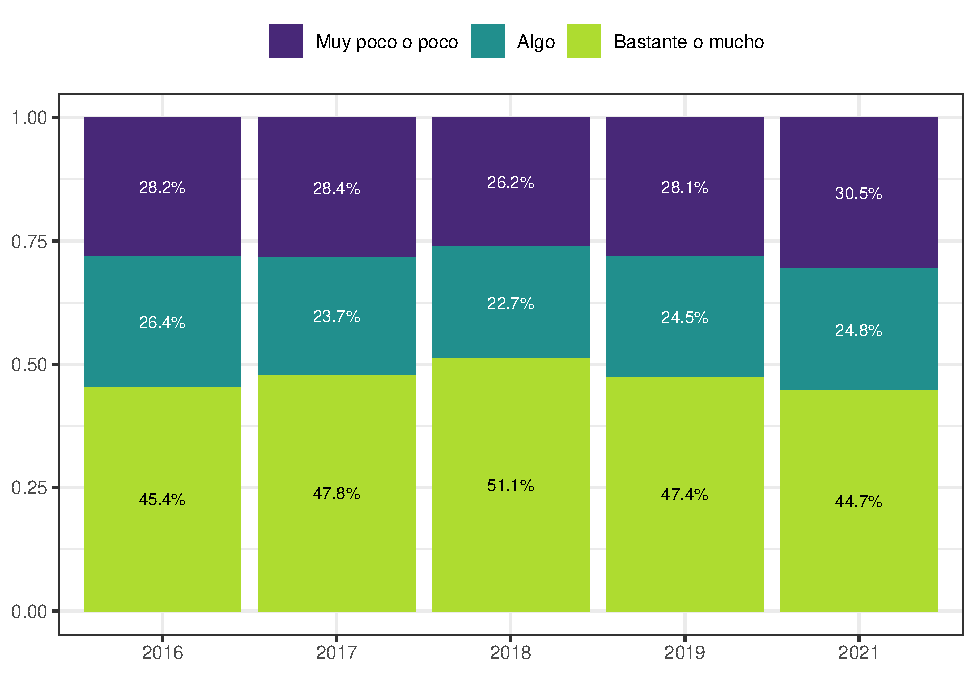
\includegraphics{reporte-elsoc_files/figure-latex/vecinos-ola-1} 

}

\caption{En términos generales, ¿cuánto confía usted en sus vecinos? según ola de estudio.}\label{fig:vecinos-ola}
\end{figure}

\begin{Shaded}
\begin{Highlighting}[]
\NormalTok{datos.}\FloatTok{8.7} \OtherTok{\textless{}{-}}\NormalTok{ elsoc\_long\_2016\_2021 }\SpecialCharTok{\%\textgreater{}\%} 
  \FunctionTok{filter}\NormalTok{(tipo\_atricion }\SpecialCharTok{==} \DecValTok{1} \SpecialCharTok{\&}\NormalTok{ muestra }\SpecialCharTok{==} \DecValTok{1} \SpecialCharTok{\&}\NormalTok{ ola }\SpecialCharTok{\%in\%} \FunctionTok{c}\NormalTok{(}\DecValTok{4}\NormalTok{,}\DecValTok{5}\NormalTok{) }\SpecialCharTok{\&} \SpecialCharTok{!}\NormalTok{t01 }\SpecialCharTok{\%in\%} \FunctionTok{c}\NormalTok{(}\SpecialCharTok{{-}}\DecValTok{888}\NormalTok{, }\SpecialCharTok{{-}}\DecValTok{999}\NormalTok{)) }\SpecialCharTok{\%\textgreater{}\%} 
  \FunctionTok{mutate}\NormalTok{(}\AttributeTok{zona1 =} \FunctionTok{factor}\NormalTok{(car}\SpecialCharTok{::}\FunctionTok{recode}\NormalTok{(region\_cod, }
                                    \StringTok{"c(1,2,3,4,15)=1; c(5,6,7,8,16)=2; c(9,10,11,12,14)=3; 13=4"}\NormalTok{),}
                        \AttributeTok{levels =} \FunctionTok{c}\NormalTok{(}\DecValTok{1}\NormalTok{,}\DecValTok{2}\NormalTok{,}\DecValTok{3}\NormalTok{,}\DecValTok{4}\NormalTok{), }
                        \AttributeTok{labels =} \FunctionTok{c}\NormalTok{(}\StringTok{"Norte"}\NormalTok{,}\StringTok{"Centro"}\NormalTok{,}\StringTok{"Sur"}\NormalTok{,}\StringTok{"Metropolitana"}\NormalTok{)))}\SpecialCharTok{\%\textgreater{}\%}
\NormalTok{  sjlabelled}\SpecialCharTok{::}\FunctionTok{as\_label}\NormalTok{(ola) }\SpecialCharTok{\%\textgreater{}\%}
  \FunctionTok{prop}\NormalTok{(}\AttributeTok{x =}\NormalTok{ t01 }\SpecialCharTok{\%in\%} \FunctionTok{c}\NormalTok{(}\DecValTok{4}\NormalTok{, }\DecValTok{5}\NormalTok{), }\AttributeTok{by =} \FunctionTok{c}\NormalTok{(ola, zona1), }\AttributeTok{na.rm =} \ConstantTok{TRUE}\NormalTok{) }

\NormalTok{g8}\FloatTok{.7} \OtherTok{\textless{}{-}}\NormalTok{ datos.}\FloatTok{8.7} \SpecialCharTok{\%\textgreater{}\%} 
  \FunctionTok{ggplot}\NormalTok{(}\FunctionTok{aes}\NormalTok{(}\AttributeTok{y =}\NormalTok{ prop, }\AttributeTok{x =}\NormalTok{ zona1, }\AttributeTok{fill =}\NormalTok{ ola, }
             \AttributeTok{label =}\NormalTok{ scales}\SpecialCharTok{::}\FunctionTok{percent}\NormalTok{(prop, }\AttributeTok{accuracy =}\NormalTok{ .}\DecValTok{1}\NormalTok{))) }\SpecialCharTok{+} 
  \FunctionTok{theme\_bw}\NormalTok{() }\SpecialCharTok{+} 
  \FunctionTok{geom\_col}\NormalTok{(}\AttributeTok{position =} \StringTok{\textquotesingle{}Dodge\textquotesingle{}}\NormalTok{) }\SpecialCharTok{+}
  \FunctionTok{scale\_y\_continuous}\NormalTok{(}\AttributeTok{labels =}\NormalTok{ scales}\SpecialCharTok{::}\NormalTok{percent,}
                     \AttributeTok{limits =} \FunctionTok{c}\NormalTok{(}\DecValTok{0}\NormalTok{, }\DecValTok{1}\NormalTok{)) }\SpecialCharTok{+}
  \FunctionTok{ylab}\NormalTok{(}\AttributeTok{label =} \ConstantTok{NULL}\NormalTok{) }\SpecialCharTok{+}
  \FunctionTok{xlab}\NormalTok{(}\AttributeTok{label =} \ConstantTok{NULL}\NormalTok{) }\SpecialCharTok{+}
  \FunctionTok{scale\_fill\_viridis\_d}\NormalTok{(}\AttributeTok{begin =} \DecValTok{0}\NormalTok{, }\AttributeTok{end =}\NormalTok{ .}\DecValTok{85}\NormalTok{, }\AttributeTok{direction =} \SpecialCharTok{{-}}\DecValTok{1}\NormalTok{, }\AttributeTok{option =} \StringTok{\textquotesingle{}viridis\textquotesingle{}}\NormalTok{) }\SpecialCharTok{+}
  \FunctionTok{theme}\NormalTok{(}\AttributeTok{legend.position =} \StringTok{\textquotesingle{}top\textquotesingle{}}\NormalTok{,}
        \AttributeTok{legend.title =} \FunctionTok{element\_blank}\NormalTok{()) }\SpecialCharTok{+}
  \FunctionTok{geom\_text}\NormalTok{(}\AttributeTok{vjust =} \SpecialCharTok{{-}}\FloatTok{0.8}\NormalTok{,}
            \AttributeTok{position =} \FunctionTok{position\_dodge}\NormalTok{(}\AttributeTok{width =}\NormalTok{ .}\DecValTok{9}\NormalTok{),}
            \AttributeTok{size=} \FloatTok{2.75}\NormalTok{)}
\NormalTok{g8}\FloatTok{.7}
\end{Highlighting}
\end{Shaded}

\begin{figure}

{\centering 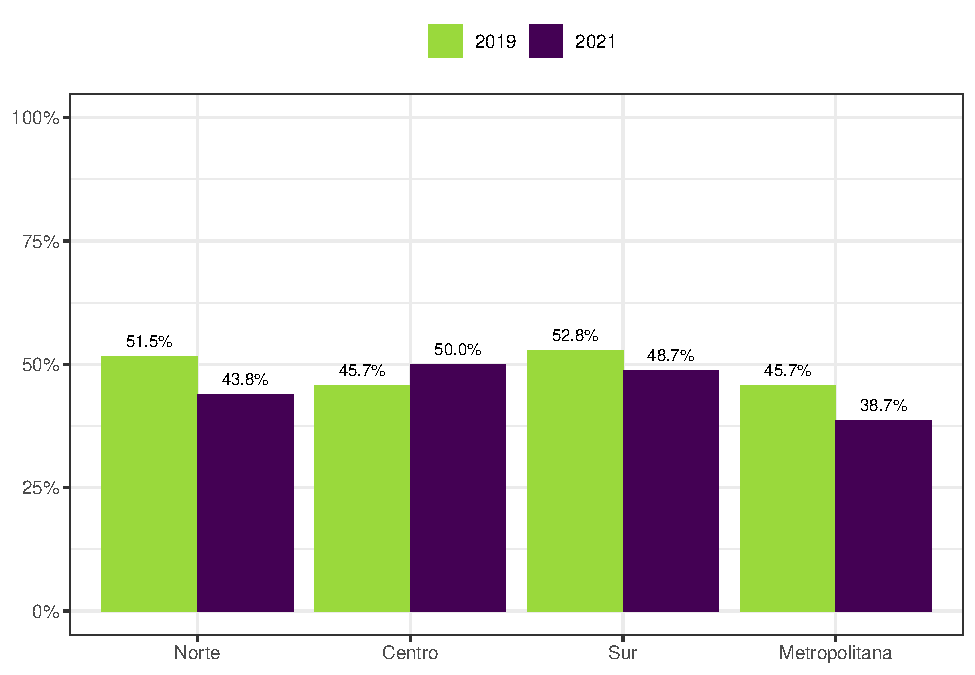
\includegraphics{reporte-elsoc_files/figure-latex/vecinos-zona-1} 

}

\caption{En términos generales, ¿cuánto confía usted en sus vecinos? Según ola del estudio y zona geográfica. Suma de Respuestas “Bastante” y “Mucho”.}\label{fig:vecinos-zona}
\end{figure}

\begin{Shaded}
\begin{Highlighting}[]
\NormalTok{datos.}\FloatTok{8.8} \OtherTok{\textless{}{-}}\NormalTok{ elsoc\_long\_2016\_2021 }\SpecialCharTok{\%\textgreater{}\%} 
  \FunctionTok{filter}\NormalTok{(tipo\_atricion }\SpecialCharTok{==} \DecValTok{1} \SpecialCharTok{\&}\NormalTok{ muestra }\SpecialCharTok{==} \DecValTok{1} \SpecialCharTok{\&}\NormalTok{ ola }\SpecialCharTok{\%in\%} \FunctionTok{c}\NormalTok{(}\DecValTok{4}\NormalTok{,}\DecValTok{5}\NormalTok{) }\SpecialCharTok{\&} \SpecialCharTok{!}\NormalTok{t01 }\SpecialCharTok{\%in\%} \FunctionTok{c}\NormalTok{(}\SpecialCharTok{{-}}\DecValTok{888}\NormalTok{, }\SpecialCharTok{{-}}\DecValTok{999}\NormalTok{)) }\SpecialCharTok{\%\textgreater{}\%} 
  \FunctionTok{mutate}\NormalTok{(}\AttributeTok{m30 =} \FunctionTok{as.numeric}\NormalTok{(car}\SpecialCharTok{::}\FunctionTok{recode}\NormalTok{(m30,}\StringTok{"1=110000;2=251000;3=305000;4=355000;5=400000;}
\StringTok{                                           6=445000;7=490000;8=535000;9=585000;10=640000;11=700000;12=765000;}
\StringTok{                                           13=845000;14=935000;15=1040000;16=1180000;17=1375000;18=1670000;}
\StringTok{                                           19=2275000;20=2700000;NA=NA"}\NormalTok{)),}
         \AttributeTok{m30b =} \FunctionTok{as.numeric}\NormalTok{(car}\SpecialCharTok{::}\FunctionTok{recode}\NormalTok{(m30b, }\StringTok{"1 = 125000; 2 = 300000; 3 = 400000; 4 = 620000; 5 = 1100000; NA = NA"}\NormalTok{)),}
         \AttributeTok{m29\_imp =} \FunctionTok{ifelse}\NormalTok{(}\SpecialCharTok{!}\FunctionTok{is.na}\NormalTok{(m29), m29, }\FunctionTok{ifelse}\NormalTok{(ola }\SpecialCharTok{==} \DecValTok{5}\NormalTok{, m30b ,m30)),}
         \AttributeTok{n\_hogar =} \FunctionTok{case\_when}\NormalTok{(ola }\SpecialCharTok{==} \DecValTok{1} \SpecialCharTok{\textasciitilde{}}\NormalTok{ nhogar1, ola }\SpecialCharTok{==} \DecValTok{2} \SpecialCharTok{\textasciitilde{}}\NormalTok{ m46\_nhogar,}
\NormalTok{                             ola }\SpecialCharTok{==} \DecValTok{3} \SpecialCharTok{\textasciitilde{}}\NormalTok{ m54, ola }\SpecialCharTok{==} \DecValTok{4} \SpecialCharTok{\textasciitilde{}}\NormalTok{ m54, ola }\SpecialCharTok{==} \DecValTok{5} \SpecialCharTok{\textasciitilde{}}\NormalTok{ m54),}
         \AttributeTok{ing\_pc =}\NormalTok{ (m29\_imp}\SpecialCharTok{/}\NormalTok{n\_hogar)) }\SpecialCharTok{\%\textgreater{}\%}
  \FunctionTok{group\_by}\NormalTok{(ola) }\SpecialCharTok{\%\textgreater{}\%} 
  \FunctionTok{mutate}\NormalTok{(}\AttributeTok{quintil =} \FunctionTok{factor}\NormalTok{(}\FunctionTok{ntile}\NormalTok{(}\SpecialCharTok{{-}}\FunctionTok{desc}\NormalTok{(ing\_pc), }\DecValTok{5}\NormalTok{), }
                          \AttributeTok{levels =} \FunctionTok{c}\NormalTok{(}\DecValTok{1}\NormalTok{,}\DecValTok{2}\NormalTok{,}\DecValTok{3}\NormalTok{,}\DecValTok{4}\NormalTok{,}\DecValTok{5}\NormalTok{),}
                          \AttributeTok{labels =} \FunctionTok{c}\NormalTok{(}\StringTok{\textquotesingle{}Q1\textquotesingle{}}\NormalTok{, }\StringTok{\textquotesingle{}Q2\textquotesingle{}}\NormalTok{, }\StringTok{\textquotesingle{}Q3\textquotesingle{}}\NormalTok{, }\StringTok{\textquotesingle{}Q4\textquotesingle{}}\NormalTok{, }\StringTok{\textquotesingle{}Q5\textquotesingle{}}\NormalTok{))) }\SpecialCharTok{\%\textgreater{}\%} 
  \FunctionTok{prop}\NormalTok{(}\AttributeTok{x =}\NormalTok{ t01 }\SpecialCharTok{\%in\%} \FunctionTok{c}\NormalTok{(}\DecValTok{4}\NormalTok{, }\DecValTok{5}\NormalTok{), }\AttributeTok{by =} \FunctionTok{c}\NormalTok{(ola, quintil), }\AttributeTok{na.rm =} \ConstantTok{TRUE}\NormalTok{) }\SpecialCharTok{\%\textgreater{}\%} 
\NormalTok{  sjlabelled}\SpecialCharTok{::}\FunctionTok{as\_label}\NormalTok{(ola)}

\NormalTok{g8}\FloatTok{.8} \OtherTok{\textless{}{-}}\NormalTok{ datos.}\FloatTok{8.8} \SpecialCharTok{\%\textgreater{}\%} 
  \FunctionTok{ggplot}\NormalTok{(}\FunctionTok{aes}\NormalTok{(}\AttributeTok{y =}\NormalTok{ prop, }\AttributeTok{x =}\NormalTok{ quintil, }\AttributeTok{fill =}\NormalTok{ ola, }
             \AttributeTok{label =}\NormalTok{ scales}\SpecialCharTok{::}\FunctionTok{percent}\NormalTok{(prop, }\AttributeTok{accuracy =}\NormalTok{ .}\DecValTok{1}\NormalTok{))) }\SpecialCharTok{+} 
  \FunctionTok{theme\_bw}\NormalTok{() }\SpecialCharTok{+} 
  \FunctionTok{geom\_col}\NormalTok{(}\AttributeTok{position =} \StringTok{\textquotesingle{}Dodge\textquotesingle{}}\NormalTok{) }\SpecialCharTok{+}
  \FunctionTok{scale\_y\_continuous}\NormalTok{(}\AttributeTok{labels =}\NormalTok{ scales}\SpecialCharTok{::}\NormalTok{percent,}
                     \AttributeTok{limits =} \FunctionTok{c}\NormalTok{(}\DecValTok{0}\NormalTok{, }\DecValTok{1}\NormalTok{)) }\SpecialCharTok{+}
  \FunctionTok{ylab}\NormalTok{(}\AttributeTok{label =} \ConstantTok{NULL}\NormalTok{) }\SpecialCharTok{+}
  \FunctionTok{xlab}\NormalTok{(}\AttributeTok{label =} \ConstantTok{NULL}\NormalTok{) }\SpecialCharTok{+}
  \FunctionTok{scale\_fill\_viridis\_d}\NormalTok{(}\AttributeTok{begin =} \DecValTok{0}\NormalTok{, }\AttributeTok{end =}\NormalTok{ .}\DecValTok{85}\NormalTok{, }\AttributeTok{direction =} \SpecialCharTok{{-}}\DecValTok{1}\NormalTok{, }\AttributeTok{option =} \StringTok{\textquotesingle{}viridis\textquotesingle{}}\NormalTok{) }\SpecialCharTok{+}
  \FunctionTok{theme}\NormalTok{(}\AttributeTok{legend.position =} \StringTok{\textquotesingle{}top\textquotesingle{}}\NormalTok{,}
        \AttributeTok{legend.title =} \FunctionTok{element\_blank}\NormalTok{()) }\SpecialCharTok{+}
  \FunctionTok{geom\_text}\NormalTok{(}\AttributeTok{vjust =} \SpecialCharTok{{-}}\FloatTok{0.8}\NormalTok{,}
            \AttributeTok{position =} \FunctionTok{position\_dodge}\NormalTok{(}\AttributeTok{width =}\NormalTok{ .}\DecValTok{9}\NormalTok{),}
            \AttributeTok{size=} \FloatTok{2.75}\NormalTok{)}
\NormalTok{g8}\FloatTok{.8}
\end{Highlighting}
\end{Shaded}

\begin{figure}

{\centering 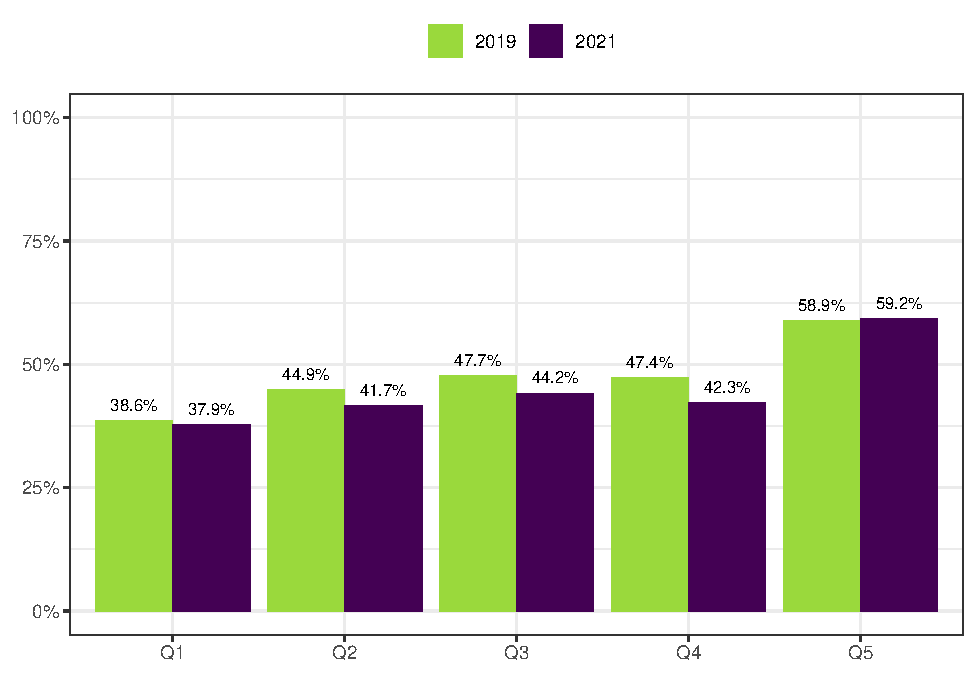
\includegraphics{reporte-elsoc_files/figure-latex/vecinos-quintil-1} 

}

\caption{En términos generales, ¿cuánto confía usted en sus vecinos? Según ola del estudio y quintil de ingreso. Suma de Respuestas “Bastante” y “Mucho”.}\label{fig:vecinos-quintil}
\end{figure}

\hypertarget{seguridad-barrial}{%
\section{Seguridad barrial}\label{seguridad-barrial}}

\begin{Shaded}
\begin{Highlighting}[]
\NormalTok{datos.}\FloatTok{8.9} \OtherTok{\textless{}{-}}\NormalTok{ elsoc\_long\_2016\_2021 }\SpecialCharTok{\%\textgreater{}\%} 
  \FunctionTok{filter}\NormalTok{(tipo\_atricion }\SpecialCharTok{==} \DecValTok{1} \SpecialCharTok{\&}\NormalTok{ muestra }\SpecialCharTok{==} \DecValTok{1} \SpecialCharTok{\&} \SpecialCharTok{!}\NormalTok{t10 }\SpecialCharTok{\%in\%} \FunctionTok{c}\NormalTok{(}\SpecialCharTok{{-}}\DecValTok{888}\NormalTok{, }\SpecialCharTok{{-}}\DecValTok{999}\NormalTok{)) }\SpecialCharTok{\%\textgreater{}\%} 
  \FunctionTok{mutate}\NormalTok{(}\AttributeTok{barrio\_segur =} \FunctionTok{factor}\NormalTok{(car}\SpecialCharTok{::}\FunctionTok{recode}\NormalTok{(t10, }\StringTok{"c(1,2)=1; c(3)=2; c(4,5)=3"}\NormalTok{), }\AttributeTok{levels =} \FunctionTok{c}\NormalTok{(}\DecValTok{1}\NormalTok{,}\DecValTok{2}\NormalTok{,}\DecValTok{3}\NormalTok{),}
                               \AttributeTok{labels =} \FunctionTok{c}\NormalTok{(}\StringTok{\textquotesingle{}Muy inseguro o inseguro\textquotesingle{}}\NormalTok{, }\StringTok{\textquotesingle{}Ni seguro ni inseguro\textquotesingle{}}\NormalTok{,}
                                          \StringTok{\textquotesingle{}Seguro o Muy seguro\textquotesingle{}}\NormalTok{))) }\SpecialCharTok{\%\textgreater{}\%}
\NormalTok{  sjlabelled}\SpecialCharTok{::}\FunctionTok{as\_label}\NormalTok{(ola) }\SpecialCharTok{\%\textgreater{}\%}
  \FunctionTok{prop}\NormalTok{(}\AttributeTok{x =}\NormalTok{ barrio\_segur, }\AttributeTok{by =}\NormalTok{ ola, }\AttributeTok{na.rm =} \ConstantTok{TRUE}\NormalTok{)}

\NormalTok{g8}\FloatTok{.9} \OtherTok{\textless{}{-}}\NormalTok{ datos.}\FloatTok{8.9} \SpecialCharTok{\%\textgreater{}\%} 
  \FunctionTok{ggplot}\NormalTok{(}\FunctionTok{aes}\NormalTok{(}\AttributeTok{y =}\NormalTok{ prop, }\AttributeTok{x =}\NormalTok{ ola, }\AttributeTok{fill =}\NormalTok{ barrio\_segur, }
             \AttributeTok{label =} \FunctionTok{as.character}\NormalTok{(scales}\SpecialCharTok{::}\FunctionTok{percent}\NormalTok{(prop, }\AttributeTok{accuracy =}\NormalTok{ .}\DecValTok{1}\NormalTok{)))) }\SpecialCharTok{+} 
  \FunctionTok{theme\_bw}\NormalTok{() }\SpecialCharTok{+} 
  \FunctionTok{geom\_col}\NormalTok{(}\AttributeTok{position =} \StringTok{\textquotesingle{}Stack\textquotesingle{}}\NormalTok{) }\SpecialCharTok{+}
  \FunctionTok{ylab}\NormalTok{(}\AttributeTok{label =} \ConstantTok{NULL}\NormalTok{) }\SpecialCharTok{+}
  \FunctionTok{xlab}\NormalTok{(}\AttributeTok{label =} \ConstantTok{NULL}\NormalTok{) }\SpecialCharTok{+}
  \FunctionTok{scale\_fill\_viridis\_d}\NormalTok{(}\AttributeTok{begin =}\NormalTok{ .}\DecValTok{11}\NormalTok{, }\AttributeTok{end =}\NormalTok{ .}\DecValTok{88}\NormalTok{, }\AttributeTok{direction =} \DecValTok{1}\NormalTok{, }\AttributeTok{option =} \StringTok{\textquotesingle{}viridis\textquotesingle{}}\NormalTok{) }\SpecialCharTok{+}
  \FunctionTok{geom\_text}\NormalTok{(}\AttributeTok{position =} \FunctionTok{position\_stack}\NormalTok{(}\AttributeTok{vjust =}\NormalTok{ .}\DecValTok{5}\NormalTok{),}
            \AttributeTok{size=} \FloatTok{2.75}\NormalTok{, }\AttributeTok{color =} \FunctionTok{rep}\NormalTok{(}\FunctionTok{c}\NormalTok{(}\StringTok{\textquotesingle{}white\textquotesingle{}}\NormalTok{, }\StringTok{\textquotesingle{}white\textquotesingle{}}\NormalTok{, }\StringTok{\textquotesingle{}black\textquotesingle{}}\NormalTok{), }\DecValTok{5}\NormalTok{)) }\SpecialCharTok{+} 
  \FunctionTok{theme}\NormalTok{(}\AttributeTok{legend.position =} \StringTok{\textquotesingle{}top\textquotesingle{}}\NormalTok{,}
        \AttributeTok{legend.title =} \FunctionTok{element\_blank}\NormalTok{())}
\NormalTok{g8}\FloatTok{.9}
\end{Highlighting}
\end{Shaded}

\begin{figure}

{\centering 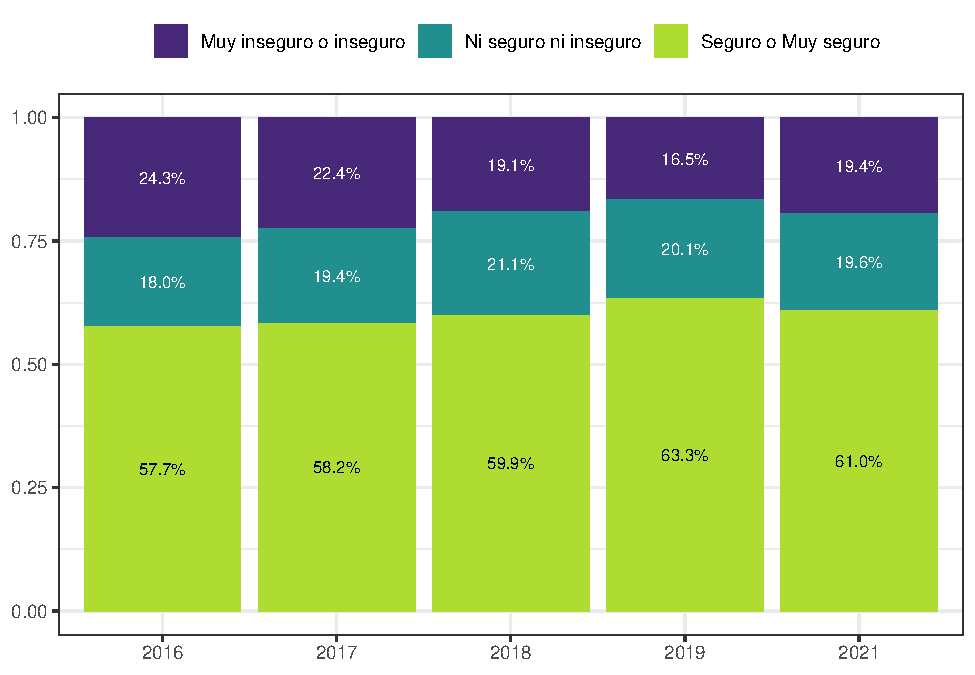
\includegraphics{reporte-elsoc_files/figure-latex/seguri-ola-1} 

}

\caption{¿Qué tan seguro o inseguro se siente en el barrio o vecindario donde usted vive? Según ola del estudio.}\label{fig:seguri-ola}
\end{figure}

\begin{Shaded}
\begin{Highlighting}[]
\NormalTok{datos.}\FloatTok{8.10} \OtherTok{\textless{}{-}}\NormalTok{ elsoc\_long\_2016\_2021 }\SpecialCharTok{\%\textgreater{}\%} 
  \FunctionTok{filter}\NormalTok{(tipo\_atricion }\SpecialCharTok{==} \DecValTok{1} \SpecialCharTok{\&}\NormalTok{ muestra }\SpecialCharTok{==} \DecValTok{1} \SpecialCharTok{\&} \SpecialCharTok{!}\NormalTok{t10 }\SpecialCharTok{\%in\%} \FunctionTok{c}\NormalTok{(}\SpecialCharTok{{-}}\DecValTok{888}\NormalTok{, }\SpecialCharTok{{-}}\DecValTok{999}\NormalTok{)) }\SpecialCharTok{\%\textgreater{}\%} 
  \FunctionTok{mutate}\NormalTok{(}\AttributeTok{zona1 =} \FunctionTok{factor}\NormalTok{(car}\SpecialCharTok{::}\FunctionTok{recode}\NormalTok{(region\_cod, }
                                    \StringTok{"c(1,2,3,4,15)=1; c(5,6,7,8,16)=2; c(9,10,11,12,14)=3; 13=4"}\NormalTok{),}
                        \AttributeTok{levels =} \FunctionTok{c}\NormalTok{(}\DecValTok{1}\NormalTok{,}\DecValTok{2}\NormalTok{,}\DecValTok{3}\NormalTok{,}\DecValTok{4}\NormalTok{), }
                        \AttributeTok{labels =} \FunctionTok{c}\NormalTok{(}\StringTok{"Norte"}\NormalTok{,}\StringTok{"Centro"}\NormalTok{,}\StringTok{"Sur"}\NormalTok{,}\StringTok{"Metropolitana"}\NormalTok{)))}\SpecialCharTok{\%\textgreater{}\%}
  \FunctionTok{prop}\NormalTok{(}\AttributeTok{x =}\NormalTok{ t10 }\SpecialCharTok{\%in\%} \FunctionTok{c}\NormalTok{(}\DecValTok{1}\NormalTok{, }\DecValTok{2}\NormalTok{), }\AttributeTok{by =} \FunctionTok{c}\NormalTok{(ola, zona1), }\AttributeTok{na.rm =} \ConstantTok{TRUE}\NormalTok{) }\SpecialCharTok{\%\textgreater{}\%} 
\NormalTok{  sjlabelled}\SpecialCharTok{::}\FunctionTok{as\_label}\NormalTok{(ola)}

\NormalTok{g8}\FloatTok{.10} \OtherTok{\textless{}{-}}\NormalTok{ datos.}\FloatTok{8.10} \SpecialCharTok{\%\textgreater{}\%} 
  \FunctionTok{ggplot}\NormalTok{(}\FunctionTok{aes}\NormalTok{(}\AttributeTok{y =}\NormalTok{ prop, }\AttributeTok{x =}\NormalTok{ ola, }\AttributeTok{color =}\NormalTok{ zona1, }\AttributeTok{group =}\NormalTok{ zona1,}
             \AttributeTok{label =} \FunctionTok{as.character}\NormalTok{(scales}\SpecialCharTok{::}\FunctionTok{percent}\NormalTok{(prop, }\AttributeTok{accuracy =}\NormalTok{ .}\DecValTok{1}\NormalTok{)))) }\SpecialCharTok{+}
  \FunctionTok{theme\_bw}\NormalTok{() }\SpecialCharTok{+}   
  \FunctionTok{geom\_line}\NormalTok{(}\AttributeTok{size =} \DecValTok{1}\NormalTok{) }\SpecialCharTok{+}
  \FunctionTok{geom\_point}\NormalTok{(}\AttributeTok{size =} \FloatTok{1.8}\NormalTok{) }\SpecialCharTok{+}
  \FunctionTok{scale\_y\_continuous}\NormalTok{(}\AttributeTok{labels =}\NormalTok{ scales}\SpecialCharTok{::}\NormalTok{percent,}
                     \AttributeTok{limits =} \FunctionTok{c}\NormalTok{(}\DecValTok{0}\NormalTok{,.}\DecValTok{5}\NormalTok{)) }\SpecialCharTok{+}
  \FunctionTok{ylab}\NormalTok{(}\AttributeTok{label =} \ConstantTok{NULL}\NormalTok{) }\SpecialCharTok{+}
  \FunctionTok{xlab}\NormalTok{(}\AttributeTok{label =} \ConstantTok{NULL}\NormalTok{) }\SpecialCharTok{+}
  \FunctionTok{scale\_color\_viridis\_d}\NormalTok{(}\AttributeTok{begin =} \DecValTok{0}\NormalTok{, }\AttributeTok{end =}\NormalTok{ .}\DecValTok{77}\NormalTok{, }\AttributeTok{direction =} \SpecialCharTok{{-}}\DecValTok{1}\NormalTok{, }\AttributeTok{option =} \StringTok{\textquotesingle{}viridis\textquotesingle{}}\NormalTok{) }\SpecialCharTok{+}
\NormalTok{  ggrepel}\SpecialCharTok{::}\FunctionTok{geom\_text\_repel}\NormalTok{(}\AttributeTok{size =} \DecValTok{3}\NormalTok{) }\SpecialCharTok{+}
  \FunctionTok{theme}\NormalTok{(}\AttributeTok{legend.position =} \StringTok{\textquotesingle{}top\textquotesingle{}}\NormalTok{,}
        \AttributeTok{legend.title =} \FunctionTok{element\_blank}\NormalTok{())}
\NormalTok{g8}\FloatTok{.10}
\end{Highlighting}
\end{Shaded}

\begin{figure}

{\centering 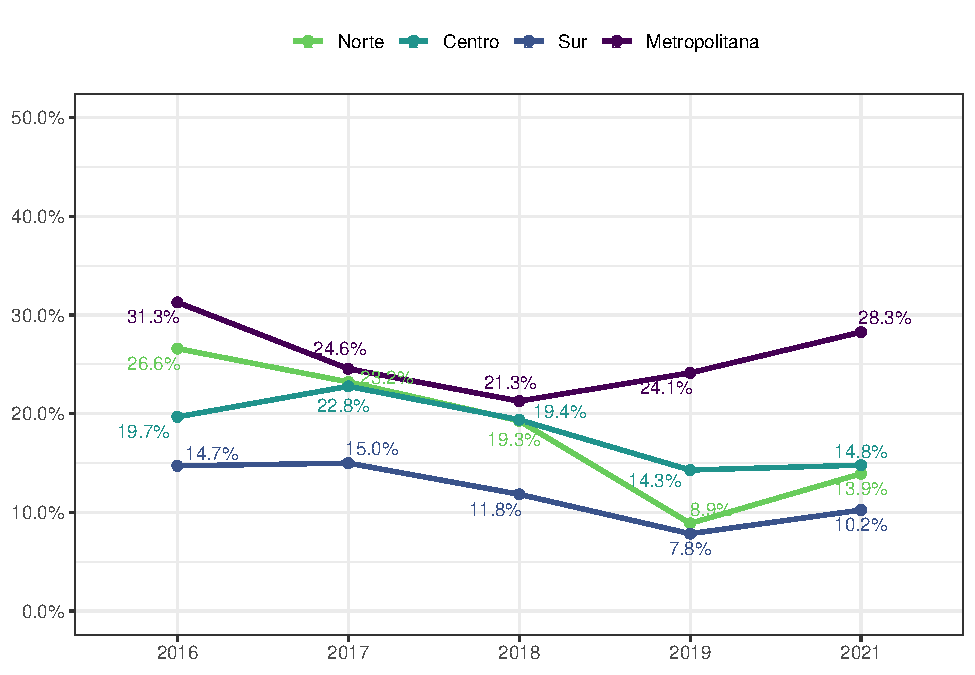
\includegraphics{reporte-elsoc_files/figure-latex/seguri-zona-1} 

}

\caption{¿Qué tan seguro o inseguro se siente en el barrio o vecindario donde usted vive? Según ola del estudio y zona geográfica. Suma de Respuestas "Inseguro" o ”Muy Inseguro".}\label{fig:seguri-zona}
\end{figure}

\begin{Shaded}
\begin{Highlighting}[]
\NormalTok{datos.}\FloatTok{8.11} \OtherTok{\textless{}{-}}\NormalTok{ elsoc\_long\_2016\_2021 }\SpecialCharTok{\%\textgreater{}\%} 
  \FunctionTok{filter}\NormalTok{(tipo\_atricion }\SpecialCharTok{==} \DecValTok{1} \SpecialCharTok{\&}\NormalTok{ muestra }\SpecialCharTok{==} \DecValTok{1} \SpecialCharTok{\&} \SpecialCharTok{!}\NormalTok{t10 }\SpecialCharTok{\%in\%} \FunctionTok{c}\NormalTok{(}\SpecialCharTok{{-}}\DecValTok{888}\NormalTok{, }\SpecialCharTok{{-}}\DecValTok{999}\NormalTok{) }\SpecialCharTok{\&} \SpecialCharTok{!}\NormalTok{m01 }\SpecialCharTok{\%in\%} \FunctionTok{c}\NormalTok{(}\SpecialCharTok{{-}}\DecValTok{888}\NormalTok{, }\SpecialCharTok{{-}}\DecValTok{999}\NormalTok{)) }\SpecialCharTok{\%\textgreater{}\%} 
  \FunctionTok{mutate}\NormalTok{(}\AttributeTok{educ =} \FunctionTok{factor}\NormalTok{(car}\SpecialCharTok{::}\FunctionTok{recode}\NormalTok{(m01,}
                                   \StringTok{"c(1,2,3)=1; c(4,5)=2; c(6,7)=3; c(8,9,10)=4"}\NormalTok{),}
                        \AttributeTok{levels =} \FunctionTok{c}\NormalTok{(}\DecValTok{1}\NormalTok{,}\DecValTok{2}\NormalTok{,}\DecValTok{3}\NormalTok{,}\DecValTok{4}\NormalTok{), }
                       \AttributeTok{labels =} \FunctionTok{c}\NormalTok{(}\StringTok{"Basica"}\NormalTok{,}\StringTok{"Media"}\NormalTok{,}\StringTok{"Tecnica"}\NormalTok{,}\StringTok{"Universitaria"}\NormalTok{))) }\SpecialCharTok{\%\textgreater{}\%}
  \FunctionTok{prop}\NormalTok{(}\AttributeTok{x =}\NormalTok{ t10 }\SpecialCharTok{\%in\%} \FunctionTok{c}\NormalTok{(}\DecValTok{1}\NormalTok{, }\DecValTok{2}\NormalTok{), }\AttributeTok{by =} \FunctionTok{c}\NormalTok{(ola, educ), }\AttributeTok{na.rm =} \ConstantTok{TRUE}\NormalTok{) }\SpecialCharTok{\%\textgreater{}\%} 
\NormalTok{  sjlabelled}\SpecialCharTok{::}\FunctionTok{as\_label}\NormalTok{(ola)}

\NormalTok{g8}\FloatTok{.11} \OtherTok{\textless{}{-}}\NormalTok{ datos.}\FloatTok{8.11} \SpecialCharTok{\%\textgreater{}\%} 
  \FunctionTok{ggplot}\NormalTok{(}\FunctionTok{aes}\NormalTok{(}\AttributeTok{y =}\NormalTok{ prop, }\AttributeTok{x =}\NormalTok{ ola, }\AttributeTok{color =}\NormalTok{ educ, }\AttributeTok{group =}\NormalTok{ educ,}
             \AttributeTok{label =} \FunctionTok{as.character}\NormalTok{(scales}\SpecialCharTok{::}\FunctionTok{percent}\NormalTok{(prop, }\AttributeTok{accuracy =}\NormalTok{ .}\DecValTok{1}\NormalTok{)))) }\SpecialCharTok{+}
  \FunctionTok{theme\_bw}\NormalTok{() }\SpecialCharTok{+}   
  \FunctionTok{geom\_line}\NormalTok{(}\AttributeTok{size =} \DecValTok{1}\NormalTok{) }\SpecialCharTok{+}
  \FunctionTok{geom\_point}\NormalTok{(}\AttributeTok{size =} \FloatTok{1.8}\NormalTok{) }\SpecialCharTok{+}
  \FunctionTok{scale\_y\_continuous}\NormalTok{(}\AttributeTok{labels =}\NormalTok{ scales}\SpecialCharTok{::}\NormalTok{percent,}
                     \AttributeTok{limits =} \FunctionTok{c}\NormalTok{(}\DecValTok{0}\NormalTok{,.}\DecValTok{5}\NormalTok{)) }\SpecialCharTok{+}
  \FunctionTok{ylab}\NormalTok{(}\AttributeTok{label =} \ConstantTok{NULL}\NormalTok{) }\SpecialCharTok{+}
  \FunctionTok{xlab}\NormalTok{(}\AttributeTok{label =} \ConstantTok{NULL}\NormalTok{) }\SpecialCharTok{+}
  \FunctionTok{scale\_color\_viridis\_d}\NormalTok{(}\AttributeTok{begin =} \DecValTok{0}\NormalTok{, }\AttributeTok{end =}\NormalTok{ .}\DecValTok{77}\NormalTok{, }\AttributeTok{direction =} \SpecialCharTok{{-}}\DecValTok{1}\NormalTok{, }\AttributeTok{option =} \StringTok{\textquotesingle{}viridis\textquotesingle{}}\NormalTok{) }\SpecialCharTok{+}
\NormalTok{  ggrepel}\SpecialCharTok{::}\FunctionTok{geom\_text\_repel}\NormalTok{(}\AttributeTok{size =} \DecValTok{3}\NormalTok{) }\SpecialCharTok{+}
  \FunctionTok{theme}\NormalTok{(}\AttributeTok{legend.position =} \StringTok{\textquotesingle{}top\textquotesingle{}}\NormalTok{,}
        \AttributeTok{legend.title =} \FunctionTok{element\_blank}\NormalTok{())}
\NormalTok{g8}\FloatTok{.11}
\end{Highlighting}
\end{Shaded}

\begin{figure}

{\centering 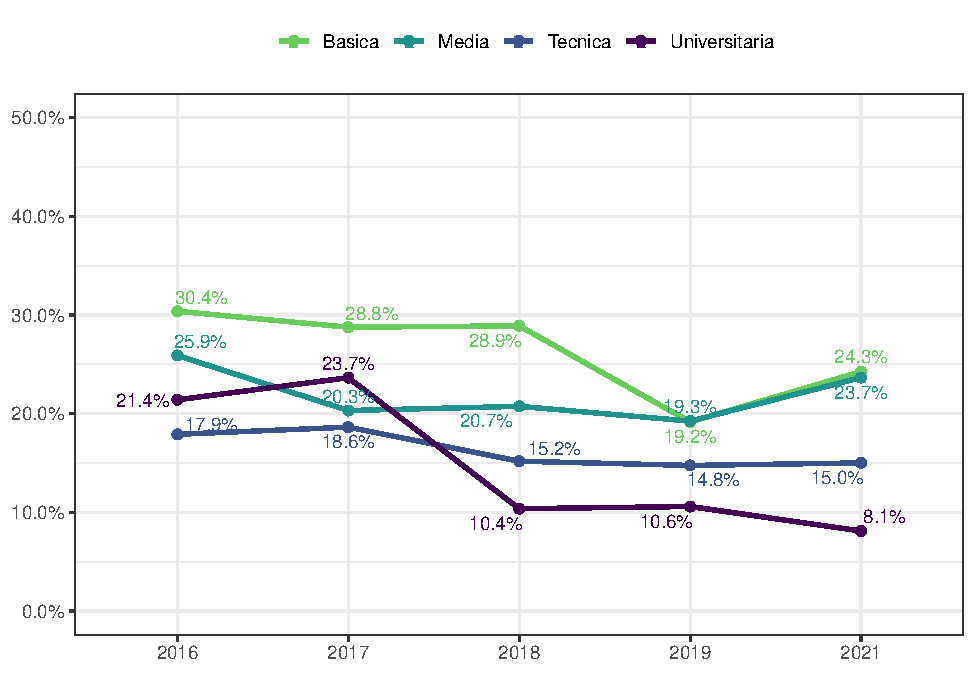
\includegraphics{reporte-elsoc_files/figure-latex/seguri-educ-1} 

}

\caption{¿Qué tan seguro o inseguro se siente en el barrio o vecindario donde usted vive? Según ola del estudio y nivel educacional. Suma de Respuestas "Inseguro" o ”Muy Inseguro".}\label{fig:seguri-educ}
\end{figure}

\begin{Shaded}
\begin{Highlighting}[]
\NormalTok{datos.}\FloatTok{8.12} \OtherTok{\textless{}{-}}\NormalTok{ elsoc\_long\_2016\_2021 }\SpecialCharTok{\%\textgreater{}\%} 
  \FunctionTok{filter}\NormalTok{(tipo\_atricion }\SpecialCharTok{==} \DecValTok{1} \SpecialCharTok{\&}\NormalTok{ muestra }\SpecialCharTok{==} \DecValTok{1} \SpecialCharTok{\&} \SpecialCharTok{!}\NormalTok{t10 }\SpecialCharTok{\%in\%} \FunctionTok{c}\NormalTok{(}\SpecialCharTok{{-}}\DecValTok{888}\NormalTok{, }\SpecialCharTok{{-}}\DecValTok{999}\NormalTok{)) }\SpecialCharTok{\%\textgreater{}\%} 
  \FunctionTok{mutate}\NormalTok{(}\AttributeTok{edadt =} \FunctionTok{factor}\NormalTok{(car}\SpecialCharTok{::}\FunctionTok{recode}\NormalTok{(m0\_edad, }
                                    \StringTok{"18:29=1;30:49=2;50:64=3;65:150=4"}\NormalTok{),}
                        \AttributeTok{levels =} \FunctionTok{c}\NormalTok{(}\DecValTok{1}\NormalTok{,}\DecValTok{2}\NormalTok{,}\DecValTok{3}\NormalTok{,}\DecValTok{4}\NormalTok{), }
                        \AttributeTok{labels =} \FunctionTok{c}\NormalTok{(}\StringTok{\textquotesingle{}18{-}29\textquotesingle{}}\NormalTok{, }\StringTok{\textquotesingle{}30{-}49\textquotesingle{}}\NormalTok{, }\StringTok{\textquotesingle{}50{-}64\textquotesingle{}}\NormalTok{, }\StringTok{\textquotesingle{}65 o más\textquotesingle{}}\NormalTok{))) }\SpecialCharTok{\%\textgreater{}\%}
\NormalTok{  sjlabelled}\SpecialCharTok{::}\FunctionTok{as\_label}\NormalTok{(ola) }\SpecialCharTok{\%\textgreater{}\%}
  \FunctionTok{prop}\NormalTok{(}\AttributeTok{x =}\NormalTok{ t10 }\SpecialCharTok{\%in\%} \FunctionTok{c}\NormalTok{(}\DecValTok{1}\NormalTok{,}\DecValTok{2}\NormalTok{), }\AttributeTok{by =} \FunctionTok{c}\NormalTok{(ola, edadt), }\AttributeTok{na.rm =} \ConstantTok{TRUE}\NormalTok{)}

\NormalTok{g8}\FloatTok{.12} \OtherTok{\textless{}{-}}\NormalTok{ datos.}\FloatTok{8.12} \SpecialCharTok{\%\textgreater{}\%} 
  \FunctionTok{ggplot}\NormalTok{(}\FunctionTok{aes}\NormalTok{(}\AttributeTok{y =}\NormalTok{ prop, }\AttributeTok{x =}\NormalTok{ ola, }\AttributeTok{color =}\NormalTok{ edadt, }\AttributeTok{group =}\NormalTok{ edadt,}
             \AttributeTok{label =} \FunctionTok{as.character}\NormalTok{(scales}\SpecialCharTok{::}\FunctionTok{percent}\NormalTok{(prop, }\AttributeTok{accuracy =}\NormalTok{ .}\DecValTok{1}\NormalTok{)))) }\SpecialCharTok{+}
  \FunctionTok{theme\_bw}\NormalTok{() }\SpecialCharTok{+}   
  \FunctionTok{geom\_line}\NormalTok{(}\AttributeTok{size =} \DecValTok{1}\NormalTok{) }\SpecialCharTok{+}
  \FunctionTok{geom\_point}\NormalTok{(}\AttributeTok{size =} \FloatTok{1.8}\NormalTok{) }\SpecialCharTok{+}
  \FunctionTok{scale\_y\_continuous}\NormalTok{(}\AttributeTok{labels =}\NormalTok{ scales}\SpecialCharTok{::}\NormalTok{percent,}
                     \AttributeTok{limits =} \FunctionTok{c}\NormalTok{(}\DecValTok{0}\NormalTok{,.}\DecValTok{5}\NormalTok{)) }\SpecialCharTok{+}
  \FunctionTok{ylab}\NormalTok{(}\AttributeTok{label =} \ConstantTok{NULL}\NormalTok{) }\SpecialCharTok{+}
  \FunctionTok{xlab}\NormalTok{(}\AttributeTok{label =} \ConstantTok{NULL}\NormalTok{) }\SpecialCharTok{+}
  \FunctionTok{scale\_color\_viridis\_d}\NormalTok{(}\AttributeTok{begin =} \DecValTok{0}\NormalTok{, }\AttributeTok{end =}\NormalTok{ .}\DecValTok{77}\NormalTok{, }\AttributeTok{direction =} \SpecialCharTok{{-}}\DecValTok{1}\NormalTok{, }\AttributeTok{option =} \StringTok{\textquotesingle{}viridis\textquotesingle{}}\NormalTok{) }\SpecialCharTok{+}
\NormalTok{  ggrepel}\SpecialCharTok{::}\FunctionTok{geom\_text\_repel}\NormalTok{(}\AttributeTok{size =} \DecValTok{3}\NormalTok{) }\SpecialCharTok{+}
  \FunctionTok{theme}\NormalTok{(}\AttributeTok{legend.position =} \StringTok{\textquotesingle{}top\textquotesingle{}}\NormalTok{,}
        \AttributeTok{legend.title =} \FunctionTok{element\_blank}\NormalTok{())}
\NormalTok{g8}\FloatTok{.12}
\end{Highlighting}
\end{Shaded}

\begin{figure}

{\centering 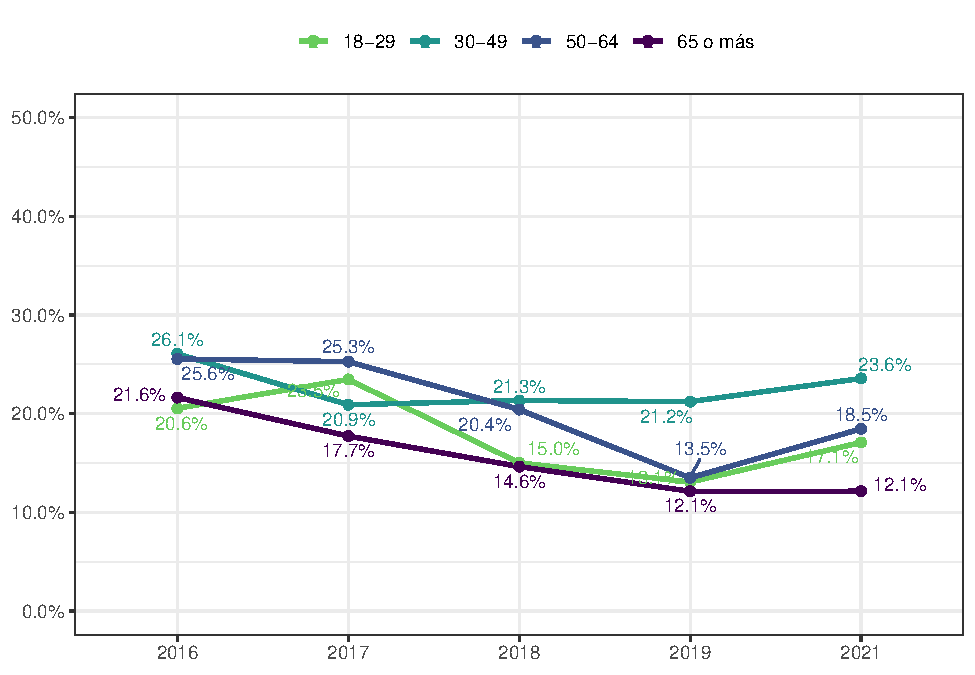
\includegraphics{reporte-elsoc_files/figure-latex/seguri-edad-1} 

}

\caption{¿Qué tan seguro o inseguro se siente en el barrio o vecindario donde usted vive? Según ola del estudio y tramos de edad. Suma de Respuestas "Inseguro" o ”Muy Inseguro".}\label{fig:seguri-edad}
\end{figure}

\begin{Shaded}
\begin{Highlighting}[]
\NormalTok{datos.}\FloatTok{8.13} \OtherTok{\textless{}{-}}\NormalTok{ elsoc\_long\_2016\_2021 }\SpecialCharTok{\%\textgreater{}\%} 
  \FunctionTok{filter}\NormalTok{(tipo\_atricion }\SpecialCharTok{==} \DecValTok{1} \SpecialCharTok{\&}\NormalTok{ muestra }\SpecialCharTok{==} \DecValTok{1} \SpecialCharTok{\&} \SpecialCharTok{!}\NormalTok{t10 }\SpecialCharTok{\%in\%} \FunctionTok{c}\NormalTok{(}\SpecialCharTok{{-}}\DecValTok{888}\NormalTok{, }\SpecialCharTok{{-}}\DecValTok{999}\NormalTok{)) }\SpecialCharTok{\%\textgreater{}\%} 
  \FunctionTok{mutate}\NormalTok{(}\AttributeTok{barrio\_segur =} \FunctionTok{factor}\NormalTok{(car}\SpecialCharTok{::}\FunctionTok{recode}\NormalTok{(t10, }\StringTok{"c(1,2)=1; c(3)=2; c(4,5)=3"}\NormalTok{), }\AttributeTok{levels =} \FunctionTok{c}\NormalTok{(}\DecValTok{1}\NormalTok{,}\DecValTok{2}\NormalTok{,}\DecValTok{3}\NormalTok{),}
                               \AttributeTok{labels =} \FunctionTok{c}\NormalTok{(}\StringTok{\textquotesingle{}Muy inseguro o inseguro\textquotesingle{}}\NormalTok{, }\StringTok{\textquotesingle{}Ni seguro ni inseguro\textquotesingle{}}\NormalTok{,}
                                          \StringTok{\textquotesingle{}Seguro o Muy seguro\textquotesingle{}}\NormalTok{)),}
         \AttributeTok{m30 =} \FunctionTok{as.numeric}\NormalTok{(car}\SpecialCharTok{::}\FunctionTok{recode}\NormalTok{(m30,}\StringTok{"1=110000;2=251000;3=305000;4=355000;5=400000;}
\StringTok{                                           6=445000;7=490000;8=535000;9=585000;10=640000;11=700000;12=765000;}
\StringTok{                                           13=845000;14=935000;15=1040000;16=1180000;17=1375000;18=1670000;}
\StringTok{                                           19=2275000;20=2700000;NA=NA"}\NormalTok{)),}
         \AttributeTok{m29\_imp =} \FunctionTok{ifelse}\NormalTok{(}\SpecialCharTok{!}\FunctionTok{is.na}\NormalTok{(m29),m29, m30),}
         \AttributeTok{n\_hogar =} \FunctionTok{case\_when}\NormalTok{(ola }\SpecialCharTok{==} \DecValTok{1} \SpecialCharTok{\textasciitilde{}}\NormalTok{ nhogar1, ola }\SpecialCharTok{==} \DecValTok{2} \SpecialCharTok{\textasciitilde{}}\NormalTok{ m46\_nhogar,}
\NormalTok{                             ola }\SpecialCharTok{==} \DecValTok{3} \SpecialCharTok{\textasciitilde{}}\NormalTok{ m54, ola }\SpecialCharTok{==} \DecValTok{4} \SpecialCharTok{\textasciitilde{}}\NormalTok{ m54, ola }\SpecialCharTok{==} \DecValTok{5} \SpecialCharTok{\textasciitilde{}}\NormalTok{ m54)) }\SpecialCharTok{\%\textgreater{}\%}
  \FunctionTok{mutate}\NormalTok{(}\AttributeTok{ing\_pc =}\NormalTok{ (m29\_imp}\SpecialCharTok{/}\NormalTok{n\_hogar)) }\SpecialCharTok{\%\textgreater{}\%}
\NormalTok{  sjlabelled}\SpecialCharTok{::}\FunctionTok{as\_label}\NormalTok{(ola) }\SpecialCharTok{\%\textgreater{}\%} 
  \FunctionTok{group\_by}\NormalTok{(ola) }\SpecialCharTok{\%\textgreater{}\%} 
  \FunctionTok{mutate}\NormalTok{(}\AttributeTok{quintil =} \FunctionTok{factor}\NormalTok{(}\FunctionTok{ntile}\NormalTok{(}\SpecialCharTok{{-}}\FunctionTok{desc}\NormalTok{(ing\_pc), }\DecValTok{5}\NormalTok{), }\AttributeTok{levels =} \FunctionTok{c}\NormalTok{(}\DecValTok{1}\NormalTok{,}\DecValTok{2}\NormalTok{,}\DecValTok{3}\NormalTok{,}\DecValTok{4}\NormalTok{,}\DecValTok{5}\NormalTok{),}
         \AttributeTok{labels =} \FunctionTok{c}\NormalTok{(}\StringTok{\textquotesingle{}Q1\textquotesingle{}}\NormalTok{, }\StringTok{\textquotesingle{}Q2\textquotesingle{}}\NormalTok{, }\StringTok{\textquotesingle{}Q3\textquotesingle{}}\NormalTok{, }\StringTok{\textquotesingle{}Q4\textquotesingle{}}\NormalTok{, }\StringTok{\textquotesingle{}Q5\textquotesingle{}}\NormalTok{))) }\SpecialCharTok{\%\textgreater{}\%} 
  \FunctionTok{prop}\NormalTok{(}\AttributeTok{x =}\NormalTok{ barrio\_segur, }\AttributeTok{by =} \FunctionTok{c}\NormalTok{(ola, quintil), }\AttributeTok{na.rm =} \ConstantTok{TRUE}\NormalTok{) }\SpecialCharTok{\%\textgreater{}\%} 
  \FunctionTok{filter}\NormalTok{(barrio\_segur }\SpecialCharTok{==} \StringTok{\textquotesingle{}Muy inseguro o inseguro\textquotesingle{}}\NormalTok{, quintil }\SpecialCharTok{==} \StringTok{"Q1"} \SpecialCharTok{|}\NormalTok{ quintil }\SpecialCharTok{==} \StringTok{"Q5"}\NormalTok{) }\SpecialCharTok{\%\textgreater{}\%} 
  \FunctionTok{drop\_na}\NormalTok{()}

\NormalTok{g8}\FloatTok{.13} \OtherTok{\textless{}{-}}\NormalTok{ datos.}\FloatTok{8.13} \SpecialCharTok{\%\textgreater{}\%} 
  \FunctionTok{ggplot}\NormalTok{(}\FunctionTok{aes}\NormalTok{(}\AttributeTok{y =}\NormalTok{ prop, }\AttributeTok{x =}\NormalTok{ ola, }\AttributeTok{color =}\NormalTok{ quintil, }\AttributeTok{group =}\NormalTok{ quintil,}
             \AttributeTok{label =} \FunctionTok{as.character}\NormalTok{(scales}\SpecialCharTok{::}\FunctionTok{percent}\NormalTok{(prop, }\AttributeTok{accuracy =}\NormalTok{ .}\DecValTok{1}\NormalTok{)))) }\SpecialCharTok{+}
  \FunctionTok{theme\_bw}\NormalTok{() }\SpecialCharTok{+}   
  \FunctionTok{geom\_line}\NormalTok{(}\AttributeTok{size =} \DecValTok{1}\NormalTok{) }\SpecialCharTok{+}
  \FunctionTok{geom\_point}\NormalTok{(}\AttributeTok{size =} \FloatTok{1.8}\NormalTok{) }\SpecialCharTok{+}
  \FunctionTok{scale\_y\_continuous}\NormalTok{(}\AttributeTok{labels =}\NormalTok{ scales}\SpecialCharTok{::}\NormalTok{percent,}
                     \AttributeTok{limits =} \FunctionTok{c}\NormalTok{(}\DecValTok{0}\NormalTok{,.}\DecValTok{5}\NormalTok{)) }\SpecialCharTok{+}
  \FunctionTok{ylab}\NormalTok{(}\AttributeTok{label =} \ConstantTok{NULL}\NormalTok{) }\SpecialCharTok{+}
  \FunctionTok{xlab}\NormalTok{(}\AttributeTok{label =} \ConstantTok{NULL}\NormalTok{) }\SpecialCharTok{+}
  \FunctionTok{scale\_color\_viridis\_d}\NormalTok{(}\AttributeTok{begin =}\NormalTok{ .}\DecValTok{0}\NormalTok{, }\AttributeTok{end =}\NormalTok{ .}\DecValTok{55}\NormalTok{, }\AttributeTok{direction =} \SpecialCharTok{{-}}\DecValTok{1}\NormalTok{, }\AttributeTok{option =} \StringTok{\textquotesingle{}viridis\textquotesingle{}}\NormalTok{) }\SpecialCharTok{+}
  \FunctionTok{geom\_text}\NormalTok{(}\AttributeTok{vjust =} \SpecialCharTok{{-}}\FloatTok{0.8}\NormalTok{,}
            \AttributeTok{size=} \FloatTok{2.75}\NormalTok{) }\SpecialCharTok{+}
  \FunctionTok{theme}\NormalTok{(}\AttributeTok{legend.position =} \StringTok{\textquotesingle{}top\textquotesingle{}}\NormalTok{,}
        \AttributeTok{legend.title =} \FunctionTok{element\_blank}\NormalTok{())}
\NormalTok{g8}\FloatTok{.13}
\end{Highlighting}
\end{Shaded}

\begin{figure}

{\centering 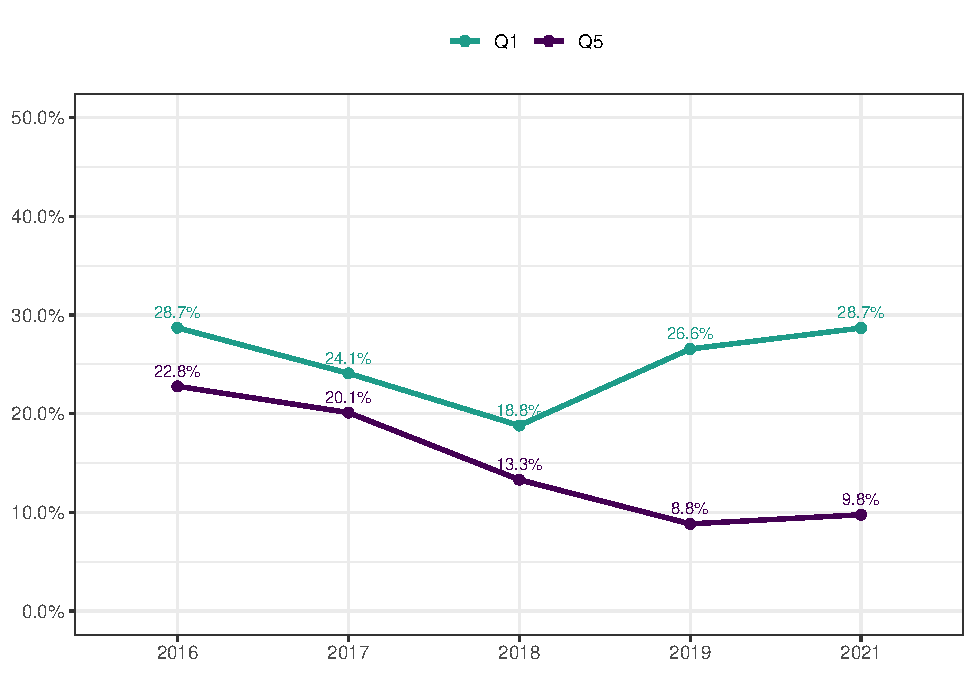
\includegraphics{reporte-elsoc_files/figure-latex/seguri-quintil-1} 

}

\caption{¿Qué tan seguro o inseguro se siente en el barrio o vecindario donde usted vive? Según ola del estudio y quintil de ingreso per capita. Suma de Respuestas "Seguro" o ”Muy Seguro".}\label{fig:seguri-quintil}
\end{figure}

\hypertarget{criminalidad-barrial}{%
\section{Criminalidad barrial}\label{criminalidad-barrial}}

\begin{Shaded}
\begin{Highlighting}[]
\NormalTok{datos.}\FloatTok{8.14} \OtherTok{\textless{}{-}}\NormalTok{ elsoc\_long\_2016\_2021 }\SpecialCharTok{\%\textgreater{}\%} 
  \FunctionTok{filter}\NormalTok{(tipo\_atricion }\SpecialCharTok{==} \DecValTok{1} \SpecialCharTok{\&}\NormalTok{ muestra }\SpecialCharTok{==} \DecValTok{1} \SpecialCharTok{\&}
           \SpecialCharTok{!}\NormalTok{t09\_01 }\SpecialCharTok{\%in\%} \FunctionTok{c}\NormalTok{(}\SpecialCharTok{{-}}\DecValTok{888}\NormalTok{, }\SpecialCharTok{{-}}\DecValTok{999}\NormalTok{) }\SpecialCharTok{\&} \SpecialCharTok{!}\NormalTok{t09\_02 }\SpecialCharTok{\%in\%} \FunctionTok{c}\NormalTok{(}\SpecialCharTok{{-}}\DecValTok{888}\NormalTok{, }\SpecialCharTok{{-}}\DecValTok{999}\NormalTok{) }\SpecialCharTok{\&} \SpecialCharTok{!}\NormalTok{t09\_03 }\SpecialCharTok{\%in\%} \FunctionTok{c}\NormalTok{(}\SpecialCharTok{{-}}\DecValTok{888}\NormalTok{, }\SpecialCharTok{{-}}\DecValTok{999}\NormalTok{)) }\SpecialCharTok{\%\textgreater{}\%} 
  \FunctionTok{mutate}\NormalTok{(}\AttributeTok{barrio\_crim =}\NormalTok{ (t09\_01 }\SpecialCharTok{+}\NormalTok{ t09\_02 }\SpecialCharTok{+}\NormalTok{ t09\_03)}\SpecialCharTok{/}\DecValTok{3}\NormalTok{) }\SpecialCharTok{\%\textgreater{}\%} 
  \FunctionTok{mutate}\NormalTok{(}\AttributeTok{barrio\_crim\_rec =} \FunctionTok{factor}\NormalTok{(}\FunctionTok{cut}\NormalTok{(barrio\_crim, }\AttributeTok{breaks =} \FunctionTok{c}\NormalTok{(}\DecValTok{0}\NormalTok{,}\DecValTok{1}\NormalTok{,}\FloatTok{2.67}\NormalTok{,}\DecValTok{5}\NormalTok{)),}
                                  \AttributeTok{labels =} \FunctionTok{c}\NormalTok{(}\StringTok{"Nunca"}\NormalTok{,}\StringTok{"Pocas o algunas veces"}\NormalTok{,}\StringTok{"Muchas veces o siempre"}\NormalTok{))) }\SpecialCharTok{\%\textgreater{}\%}
\NormalTok{  sjlabelled}\SpecialCharTok{::}\FunctionTok{as\_label}\NormalTok{(ola) }\SpecialCharTok{\%\textgreater{}\%} 
  \FunctionTok{prop}\NormalTok{(}\AttributeTok{x =}\NormalTok{ barrio\_crim\_rec, }\AttributeTok{by =}\NormalTok{ ola, }\AttributeTok{na.rm =} \ConstantTok{TRUE}\NormalTok{)}

\NormalTok{g8}\FloatTok{.14} \OtherTok{\textless{}{-}}\NormalTok{ datos.}\FloatTok{8.14} \SpecialCharTok{\%\textgreater{}\%} 
  \FunctionTok{ggplot}\NormalTok{(}\FunctionTok{aes}\NormalTok{(}\AttributeTok{y =}\NormalTok{ prop, }\AttributeTok{x =}\NormalTok{ ola, }\AttributeTok{fill =}\NormalTok{ barrio\_crim\_rec, }
             \AttributeTok{label =} \FunctionTok{as.character}\NormalTok{(scales}\SpecialCharTok{::}\FunctionTok{percent}\NormalTok{(prop, }\AttributeTok{accuracy =}\NormalTok{ .}\DecValTok{1}\NormalTok{)))) }\SpecialCharTok{+} 
  \FunctionTok{theme\_bw}\NormalTok{() }\SpecialCharTok{+} 
  \FunctionTok{geom\_col}\NormalTok{(}\AttributeTok{position =} \StringTok{\textquotesingle{}Stack\textquotesingle{}}\NormalTok{) }\SpecialCharTok{+}
  \FunctionTok{ylab}\NormalTok{(}\AttributeTok{label =} \ConstantTok{NULL}\NormalTok{) }\SpecialCharTok{+}
  \FunctionTok{xlab}\NormalTok{(}\AttributeTok{label =} \ConstantTok{NULL}\NormalTok{) }\SpecialCharTok{+}
  \FunctionTok{scale\_fill\_viridis\_d}\NormalTok{(}\AttributeTok{begin =}\NormalTok{ .}\DecValTok{11}\NormalTok{, }\AttributeTok{end =}\NormalTok{ .}\DecValTok{88}\NormalTok{, }\AttributeTok{direction =} \SpecialCharTok{{-}}\DecValTok{1}\NormalTok{, }\AttributeTok{option =} \StringTok{\textquotesingle{}viridis\textquotesingle{}}\NormalTok{) }\SpecialCharTok{+}
  \FunctionTok{geom\_text}\NormalTok{(}\AttributeTok{position =} \FunctionTok{position\_stack}\NormalTok{(}\AttributeTok{vjust =}\NormalTok{ .}\DecValTok{5}\NormalTok{),}
            \AttributeTok{size=} \FloatTok{2.75}\NormalTok{, }\AttributeTok{color =} \FunctionTok{rep}\NormalTok{(}\FunctionTok{c}\NormalTok{(}\StringTok{\textquotesingle{}black\textquotesingle{}}\NormalTok{, }\StringTok{\textquotesingle{}white\textquotesingle{}}\NormalTok{, }\StringTok{\textquotesingle{}white\textquotesingle{}}\NormalTok{), }\DecValTok{5}\NormalTok{)) }\SpecialCharTok{+} 
  \FunctionTok{theme}\NormalTok{(}\AttributeTok{legend.position =} \StringTok{\textquotesingle{}top\textquotesingle{}}\NormalTok{, }\AttributeTok{legend.title =} \FunctionTok{element\_blank}\NormalTok{())}
\NormalTok{g8}\FloatTok{.14}
\end{Highlighting}
\end{Shaded}

\begin{figure}

{\centering 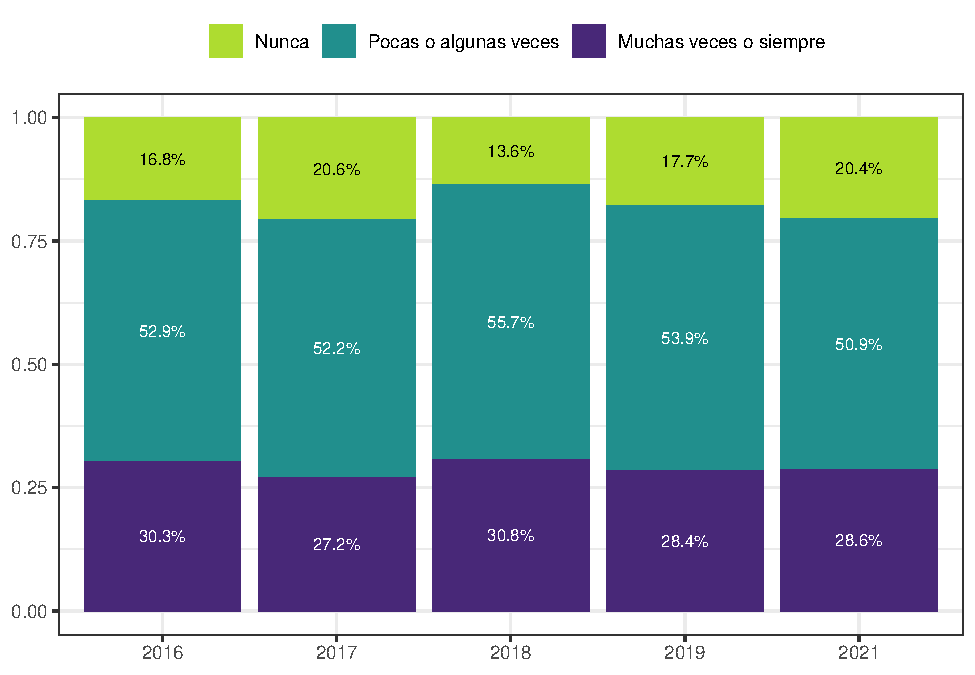
\includegraphics{reporte-elsoc_files/figure-latex/crim-olas-1} 

}

\caption{¿Con qué frecuencia se han producido crímenes (riñas, robos y tráfico de drogas) en su barrio?, según ola de estudio.}\label{fig:crim-olas}
\end{figure}

\begin{Shaded}
\begin{Highlighting}[]
\NormalTok{datos.}\FloatTok{8.15} \OtherTok{\textless{}{-}}\NormalTok{ elsoc\_long\_2016\_2021 }\SpecialCharTok{\%\textgreater{}\%} 
  \FunctionTok{filter}\NormalTok{(tipo\_atricion }\SpecialCharTok{==} \DecValTok{1} \SpecialCharTok{\&}\NormalTok{ muestra }\SpecialCharTok{==} \DecValTok{1} \SpecialCharTok{\&}\NormalTok{ ola }\SpecialCharTok{\%in\%} \FunctionTok{c}\NormalTok{(}\DecValTok{4}\NormalTok{,}\DecValTok{5}\NormalTok{) }\SpecialCharTok{\&}
           \SpecialCharTok{!}\NormalTok{t09\_01 }\SpecialCharTok{\%in\%} \FunctionTok{c}\NormalTok{(}\SpecialCharTok{{-}}\DecValTok{888}\NormalTok{, }\SpecialCharTok{{-}}\DecValTok{999}\NormalTok{) }\SpecialCharTok{\&} \SpecialCharTok{!}\NormalTok{t09\_02 }\SpecialCharTok{\%in\%} \FunctionTok{c}\NormalTok{(}\SpecialCharTok{{-}}\DecValTok{888}\NormalTok{, }\SpecialCharTok{{-}}\DecValTok{999}\NormalTok{) }\SpecialCharTok{\&} \SpecialCharTok{!}\NormalTok{t09\_03 }\SpecialCharTok{\%in\%} \FunctionTok{c}\NormalTok{(}\SpecialCharTok{{-}}\DecValTok{888}\NormalTok{, }\SpecialCharTok{{-}}\DecValTok{999}\NormalTok{)) }\SpecialCharTok{\%\textgreater{}\%} 
  \FunctionTok{mutate}\NormalTok{(}\AttributeTok{barrio\_crim =}\NormalTok{ (t09\_01 }\SpecialCharTok{+}\NormalTok{ t09\_02 }\SpecialCharTok{+}\NormalTok{ t09\_03)}\SpecialCharTok{/}\DecValTok{3}\NormalTok{) }\SpecialCharTok{\%\textgreater{}\%} 
  \FunctionTok{mutate}\NormalTok{(}\AttributeTok{barrio\_crim\_rec =} \FunctionTok{factor}\NormalTok{(}\FunctionTok{cut}\NormalTok{(barrio\_crim, }\AttributeTok{breaks =} \FunctionTok{c}\NormalTok{(}\DecValTok{0}\NormalTok{,}\DecValTok{1}\NormalTok{,}\FloatTok{2.67}\NormalTok{,}\DecValTok{5}\NormalTok{)),}
                                  \AttributeTok{labels =} \FunctionTok{c}\NormalTok{(}\StringTok{"Nunca"}\NormalTok{,}\StringTok{"Pocas o algunas veces"}\NormalTok{,}\StringTok{"Muchas veces o siempre"}\NormalTok{)),}
         \AttributeTok{zona1 =} \FunctionTok{factor}\NormalTok{(car}\SpecialCharTok{::}\FunctionTok{recode}\NormalTok{(region\_cod, }\StringTok{"c(1,2,3,4,15)=1; c(5,6,7,8,16)=2; c(9,10,11,12,14)=3; 13=4"}\NormalTok{),}
                        \AttributeTok{levels =} \FunctionTok{c}\NormalTok{(}\DecValTok{1}\NormalTok{,}\DecValTok{2}\NormalTok{,}\DecValTok{3}\NormalTok{,}\DecValTok{4}\NormalTok{), }\AttributeTok{labels =} \FunctionTok{c}\NormalTok{(}\StringTok{"Norte"}\NormalTok{,}\StringTok{"Centro"}\NormalTok{,}\StringTok{"Sur"}\NormalTok{,}\StringTok{"Metropolitana"}\NormalTok{))) }\SpecialCharTok{\%\textgreater{}\%}
\NormalTok{  sjlabelled}\SpecialCharTok{::}\FunctionTok{as\_label}\NormalTok{(ola) }\SpecialCharTok{\%\textgreater{}\%} 
  \FunctionTok{prop}\NormalTok{(}\AttributeTok{x =}\NormalTok{ barrio\_crim\_rec, }\AttributeTok{by =} \FunctionTok{c}\NormalTok{(ola, zona1), }\AttributeTok{na.rm =} \ConstantTok{TRUE}\NormalTok{) }\SpecialCharTok{\%\textgreater{}\%} 
  \FunctionTok{filter}\NormalTok{(barrio\_crim\_rec }\SpecialCharTok{==} \StringTok{\textquotesingle{}Muchas veces o siempre\textquotesingle{}}\NormalTok{)}

\NormalTok{g8}\FloatTok{.15} \OtherTok{\textless{}{-}}\NormalTok{ datos.}\FloatTok{8.15} \SpecialCharTok{\%\textgreater{}\%} 
  \FunctionTok{ggplot}\NormalTok{(}\FunctionTok{aes}\NormalTok{(}\AttributeTok{y =}\NormalTok{ prop, }\AttributeTok{x =}\NormalTok{ zona1, }\AttributeTok{fill =}\NormalTok{ ola, }
             \AttributeTok{label =} \FunctionTok{as.character}\NormalTok{(scales}\SpecialCharTok{::}\FunctionTok{percent}\NormalTok{(prop, }\AttributeTok{accuracy =}\NormalTok{ .}\DecValTok{1}\NormalTok{)))) }\SpecialCharTok{+} 
  \FunctionTok{theme\_bw}\NormalTok{() }\SpecialCharTok{+} 
  \FunctionTok{geom\_col}\NormalTok{(}\AttributeTok{position =} \StringTok{\textquotesingle{}Dodge\textquotesingle{}}\NormalTok{) }\SpecialCharTok{+}
  \FunctionTok{scale\_y\_continuous}\NormalTok{(}\AttributeTok{labels =}\NormalTok{ scales}\SpecialCharTok{::}\NormalTok{percent,}
                     \AttributeTok{limits =} \FunctionTok{c}\NormalTok{(}\DecValTok{0}\NormalTok{, .}\DecValTok{5}\NormalTok{)) }\SpecialCharTok{+}
  \FunctionTok{ylab}\NormalTok{(}\AttributeTok{label =} \ConstantTok{NULL}\NormalTok{) }\SpecialCharTok{+}
  \FunctionTok{xlab}\NormalTok{(}\AttributeTok{label =} \ConstantTok{NULL}\NormalTok{) }\SpecialCharTok{+}
  \FunctionTok{scale\_fill\_viridis\_d}\NormalTok{(}\AttributeTok{begin =} \DecValTok{0}\NormalTok{, }\AttributeTok{end =}\NormalTok{ .}\DecValTok{85}\NormalTok{, }\AttributeTok{direction =} \SpecialCharTok{{-}}\DecValTok{1}\NormalTok{, }\AttributeTok{option =} \StringTok{\textquotesingle{}viridis\textquotesingle{}}\NormalTok{) }\SpecialCharTok{+}
  \FunctionTok{theme}\NormalTok{(}\AttributeTok{legend.position =} \StringTok{\textquotesingle{}top\textquotesingle{}}\NormalTok{,}
        \AttributeTok{legend.title =} \FunctionTok{element\_blank}\NormalTok{()) }\SpecialCharTok{+}
  \FunctionTok{geom\_text}\NormalTok{(}\AttributeTok{vjust =} \SpecialCharTok{{-}}\FloatTok{0.8}\NormalTok{,}
            \AttributeTok{position =} \FunctionTok{position\_dodge}\NormalTok{(}\AttributeTok{width =}\NormalTok{ .}\DecValTok{9}\NormalTok{),}
            \AttributeTok{size=} \FloatTok{2.75}\NormalTok{)}
\NormalTok{g8}\FloatTok{.15}
\end{Highlighting}
\end{Shaded}

\begin{figure}

{\centering 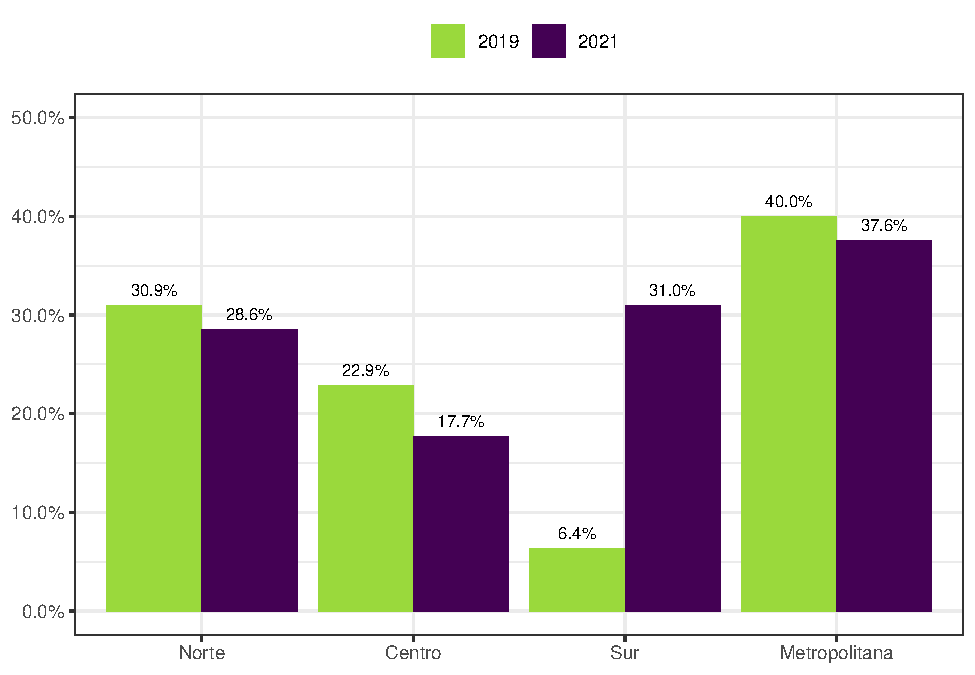
\includegraphics{reporte-elsoc_files/figure-latex/crim-zona-1} 

}

\caption{¿Con qué frecuencia se han producido crímenes (riñas, robos y tráfico de drogas) en su barrio?, según ola del estudio y zona geográfica. Porcentaje de experiencias de criminalidad "Siempre" o "Muchas veces".}\label{fig:crim-zona}
\end{figure}

\begin{Shaded}
\begin{Highlighting}[]
\NormalTok{datos.}\FloatTok{8.16} \OtherTok{\textless{}{-}}\NormalTok{ elsoc\_long\_2016\_2021 }\SpecialCharTok{\%\textgreater{}\%} 
  \FunctionTok{filter}\NormalTok{(tipo\_atricion }\SpecialCharTok{==} \DecValTok{1} \SpecialCharTok{\&}\NormalTok{ muestra }\SpecialCharTok{==} \DecValTok{1} \SpecialCharTok{\&}\NormalTok{ ola }\SpecialCharTok{\%in\%} \FunctionTok{c}\NormalTok{(}\DecValTok{4}\NormalTok{,}\DecValTok{5}\NormalTok{) }\SpecialCharTok{\&}
           \SpecialCharTok{!}\NormalTok{t09\_01 }\SpecialCharTok{\%in\%} \FunctionTok{c}\NormalTok{(}\SpecialCharTok{{-}}\DecValTok{888}\NormalTok{, }\SpecialCharTok{{-}}\DecValTok{999}\NormalTok{) }\SpecialCharTok{\&} \SpecialCharTok{!}\NormalTok{t09\_02 }\SpecialCharTok{\%in\%} \FunctionTok{c}\NormalTok{(}\SpecialCharTok{{-}}\DecValTok{888}\NormalTok{, }\SpecialCharTok{{-}}\DecValTok{999}\NormalTok{) }\SpecialCharTok{\&} \SpecialCharTok{!}\NormalTok{t09\_03 }\SpecialCharTok{\%in\%} \FunctionTok{c}\NormalTok{(}\SpecialCharTok{{-}}\DecValTok{888}\NormalTok{, }\SpecialCharTok{{-}}\DecValTok{999}\NormalTok{)) }\SpecialCharTok{\%\textgreater{}\%} 
  \FunctionTok{mutate}\NormalTok{(}\AttributeTok{barrio\_crim =}\NormalTok{ (t09\_01 }\SpecialCharTok{+}\NormalTok{ t09\_02 }\SpecialCharTok{+}\NormalTok{ t09\_03)}\SpecialCharTok{/}\DecValTok{3}\NormalTok{) }\SpecialCharTok{\%\textgreater{}\%} 
  \FunctionTok{mutate}\NormalTok{(}\AttributeTok{barrio\_crim\_rec =} \FunctionTok{factor}\NormalTok{(}\FunctionTok{cut}\NormalTok{(barrio\_crim, }\AttributeTok{breaks =} \FunctionTok{c}\NormalTok{(}\DecValTok{0}\NormalTok{,}\DecValTok{1}\NormalTok{,}\FloatTok{2.67}\NormalTok{,}\DecValTok{5}\NormalTok{)),}
                                  \AttributeTok{labels =} \FunctionTok{c}\NormalTok{(}\StringTok{"Nunca"}\NormalTok{,}\StringTok{"Pocas o algunas veces"}\NormalTok{,}\StringTok{"Muchas veces o siempre"}\NormalTok{)),}
         \AttributeTok{estrato =} \FunctionTok{factor}\NormalTok{(estrato, }\AttributeTok{levels =} \FunctionTok{c}\NormalTok{(}\DecValTok{1}\NormalTok{,}\DecValTok{2}\NormalTok{,}\DecValTok{3}\NormalTok{,}\DecValTok{4}\NormalTok{,}\DecValTok{5}\NormalTok{,}\DecValTok{6}\NormalTok{),}
                          \AttributeTok{labels =} \FunctionTok{c}\NormalTok{(}\StringTok{\textquotesingle{}Gran}\SpecialCharTok{\textbackslash{}n}\StringTok{Santiago\textquotesingle{}}\NormalTok{, }\StringTok{\textquotesingle{}Gran}\SpecialCharTok{\textbackslash{}n}\StringTok{Valparaíso\textquotesingle{}}\NormalTok{, }\StringTok{\textquotesingle{}Gran}\SpecialCharTok{\textbackslash{}n}\StringTok{Concepción\textquotesingle{}}\NormalTok{,}
                                     \StringTok{\textquotesingle{}Ciudades}\SpecialCharTok{\textbackslash{}n}\StringTok{grandes\textquotesingle{}}\NormalTok{, }\StringTok{\textquotesingle{}Ciudades}\SpecialCharTok{\textbackslash{}n}\StringTok{medianas\textquotesingle{}}\NormalTok{, }\StringTok{\textquotesingle{}Ciudades}\SpecialCharTok{\textbackslash{}n}\StringTok{pequeñas\textquotesingle{}}\NormalTok{))) }\SpecialCharTok{\%\textgreater{}\%}
\NormalTok{  sjlabelled}\SpecialCharTok{::}\FunctionTok{as\_label}\NormalTok{(ola) }\SpecialCharTok{\%\textgreater{}\%} 
  \FunctionTok{prop}\NormalTok{(}\AttributeTok{x =}\NormalTok{ barrio\_crim\_rec, }\AttributeTok{by =} \FunctionTok{c}\NormalTok{(ola, estrato), }\AttributeTok{na.rm =} \ConstantTok{TRUE}\NormalTok{) }\SpecialCharTok{\%\textgreater{}\%} 
  \FunctionTok{filter}\NormalTok{(barrio\_crim\_rec }\SpecialCharTok{==} \StringTok{\textquotesingle{}Muchas veces o siempre\textquotesingle{}}\NormalTok{)}

\NormalTok{g8}\FloatTok{.16} \OtherTok{\textless{}{-}}\NormalTok{ datos.}\FloatTok{8.16} \SpecialCharTok{\%\textgreater{}\%} 
  \FunctionTok{ggplot}\NormalTok{(}\FunctionTok{aes}\NormalTok{(}\AttributeTok{y =}\NormalTok{ prop, }\AttributeTok{x =}\NormalTok{ estrato, }\AttributeTok{fill =}\NormalTok{ ola, }
             \AttributeTok{label =} \FunctionTok{as.character}\NormalTok{(scales}\SpecialCharTok{::}\FunctionTok{percent}\NormalTok{(prop, }\AttributeTok{accuracy =}\NormalTok{ .}\DecValTok{1}\NormalTok{)))) }\SpecialCharTok{+} 
  \FunctionTok{theme\_bw}\NormalTok{() }\SpecialCharTok{+} 
  \FunctionTok{geom\_col}\NormalTok{(}\AttributeTok{position =} \StringTok{\textquotesingle{}Dodge\textquotesingle{}}\NormalTok{) }\SpecialCharTok{+}
  \FunctionTok{scale\_y\_continuous}\NormalTok{(}\AttributeTok{labels =}\NormalTok{ scales}\SpecialCharTok{::}\NormalTok{percent,}
                     \AttributeTok{limits =} \FunctionTok{c}\NormalTok{(}\DecValTok{0}\NormalTok{, .}\DecValTok{5}\NormalTok{)) }\SpecialCharTok{+}
  \FunctionTok{ylab}\NormalTok{(}\AttributeTok{label =} \ConstantTok{NULL}\NormalTok{) }\SpecialCharTok{+}
  \FunctionTok{xlab}\NormalTok{(}\AttributeTok{label =} \ConstantTok{NULL}\NormalTok{) }\SpecialCharTok{+}
  \FunctionTok{scale\_fill\_viridis\_d}\NormalTok{(}\AttributeTok{begin =} \DecValTok{0}\NormalTok{, }\AttributeTok{end =}\NormalTok{ .}\DecValTok{85}\NormalTok{, }\AttributeTok{direction =} \SpecialCharTok{{-}}\DecValTok{1}\NormalTok{, }\AttributeTok{option =} \StringTok{\textquotesingle{}viridis\textquotesingle{}}\NormalTok{) }\SpecialCharTok{+}
  \FunctionTok{theme}\NormalTok{(}\AttributeTok{legend.position =} \StringTok{\textquotesingle{}top\textquotesingle{}}\NormalTok{,}
        \AttributeTok{legend.title =} \FunctionTok{element\_blank}\NormalTok{()) }\SpecialCharTok{+}
  \FunctionTok{geom\_text}\NormalTok{(}\AttributeTok{vjust =} \SpecialCharTok{{-}}\FloatTok{0.8}\NormalTok{,}
            \AttributeTok{position =} \FunctionTok{position\_dodge}\NormalTok{(}\AttributeTok{width =}\NormalTok{ .}\DecValTok{9}\NormalTok{),}
            \AttributeTok{size=} \FloatTok{2.75}\NormalTok{)}
\NormalTok{g8}\FloatTok{.16}
\end{Highlighting}
\end{Shaded}

\begin{figure}

{\centering 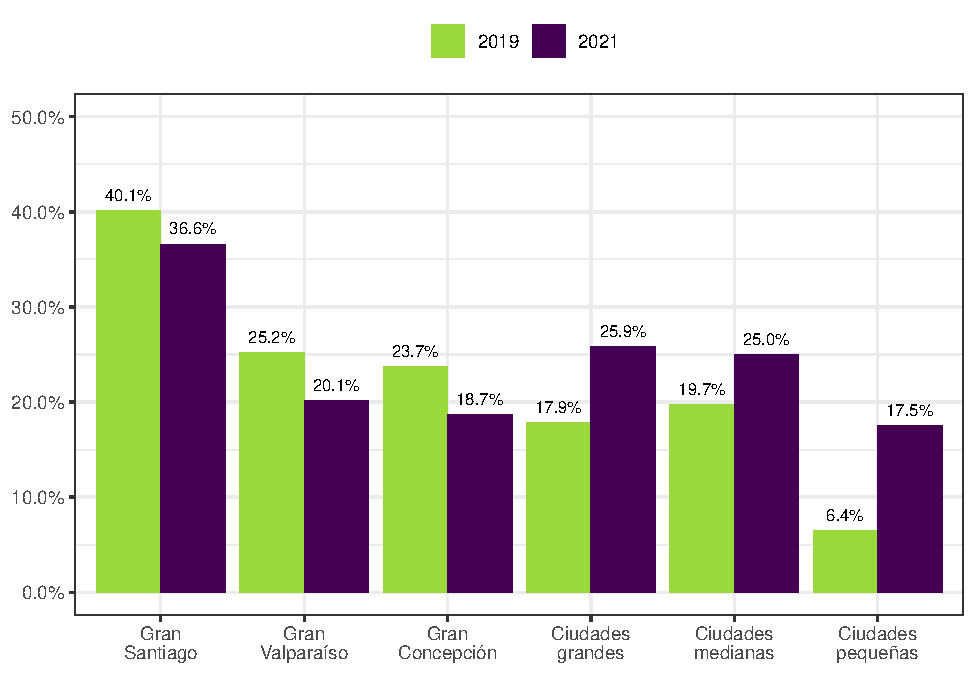
\includegraphics{reporte-elsoc_files/figure-latex/crim-estrato-1} 

}

\caption{¿Con qué frecuencia se han producido crímenes (riñas, robos y tráfico de drogas) en su barrio?, según ola del estudio y tipo de ciudad. Porcentaje de experiencias de criminalidad "Siempre" o "Muchas veces".}\label{fig:crim-estrato}
\end{figure}

\begin{Shaded}
\begin{Highlighting}[]
\NormalTok{datos.}\FloatTok{8.17} \OtherTok{\textless{}{-}}\NormalTok{ elsoc\_long\_2016\_2021 }\SpecialCharTok{\%\textgreater{}\%} 
  \FunctionTok{filter}\NormalTok{(tipo\_atricion }\SpecialCharTok{==} \DecValTok{1} \SpecialCharTok{\&}\NormalTok{ muestra }\SpecialCharTok{==} \DecValTok{1} \SpecialCharTok{\&}
           \SpecialCharTok{!}\NormalTok{t09\_01 }\SpecialCharTok{\%in\%} \FunctionTok{c}\NormalTok{(}\SpecialCharTok{{-}}\DecValTok{888}\NormalTok{, }\SpecialCharTok{{-}}\DecValTok{999}\NormalTok{) }\SpecialCharTok{\&} \SpecialCharTok{!}\NormalTok{t09\_02 }\SpecialCharTok{\%in\%} \FunctionTok{c}\NormalTok{(}\SpecialCharTok{{-}}\DecValTok{888}\NormalTok{, }\SpecialCharTok{{-}}\DecValTok{999}\NormalTok{) }\SpecialCharTok{\&} \SpecialCharTok{!}\NormalTok{t09\_03 }\SpecialCharTok{\%in\%} \FunctionTok{c}\NormalTok{(}\SpecialCharTok{{-}}\DecValTok{888}\NormalTok{, }\SpecialCharTok{{-}}\DecValTok{999}\NormalTok{)) }\SpecialCharTok{\%\textgreater{}\%} 
  \FunctionTok{mutate}\NormalTok{(}\AttributeTok{barrio\_crim =}\NormalTok{ (t09\_01 }\SpecialCharTok{+}\NormalTok{ t09\_02 }\SpecialCharTok{+}\NormalTok{ t09\_03)}\SpecialCharTok{/}\DecValTok{3}\NormalTok{) }\SpecialCharTok{\%\textgreater{}\%} 
  \FunctionTok{mutate}\NormalTok{(}\AttributeTok{barrio\_crim\_rec =} \FunctionTok{factor}\NormalTok{(}\FunctionTok{cut}\NormalTok{(barrio\_crim, }\AttributeTok{breaks =} \FunctionTok{c}\NormalTok{(}\DecValTok{0}\NormalTok{,}\DecValTok{1}\NormalTok{,}\FloatTok{2.67}\NormalTok{,}\DecValTok{5}\NormalTok{)),}
                                  \AttributeTok{labels =} \FunctionTok{c}\NormalTok{(}\StringTok{"Nunca"}\NormalTok{,}\StringTok{"Pocas o algunas veces"}\NormalTok{,}\StringTok{"Muchas veces o siempre"}\NormalTok{)),}
         \AttributeTok{m30 =} \FunctionTok{as.numeric}\NormalTok{(car}\SpecialCharTok{::}\FunctionTok{recode}\NormalTok{(m30,}\StringTok{"1=110000;2=251000;3=305000;4=355000;5=400000;}
\StringTok{                                           6=445000;7=490000;8=535000;9=585000;10=640000;11=700000;12=765000;}
\StringTok{                                           13=845000;14=935000;15=1040000;16=1180000;17=1375000;18=1670000;}
\StringTok{                                           19=2275000;20=2700000;NA=NA"}\NormalTok{)),}
         \AttributeTok{m29\_imp =} \FunctionTok{ifelse}\NormalTok{(}\SpecialCharTok{!}\FunctionTok{is.na}\NormalTok{(m29),m29, m30),}
         \AttributeTok{n\_hogar =} \FunctionTok{case\_when}\NormalTok{(ola }\SpecialCharTok{==} \DecValTok{1} \SpecialCharTok{\textasciitilde{}}\NormalTok{ nhogar1, ola }\SpecialCharTok{==} \DecValTok{2} \SpecialCharTok{\textasciitilde{}}\NormalTok{ m46\_nhogar,}
\NormalTok{                             ola }\SpecialCharTok{==} \DecValTok{3} \SpecialCharTok{\textasciitilde{}}\NormalTok{ m54, ola }\SpecialCharTok{==} \DecValTok{4} \SpecialCharTok{\textasciitilde{}}\NormalTok{ m54, ola }\SpecialCharTok{==} \DecValTok{5} \SpecialCharTok{\textasciitilde{}}\NormalTok{ m54)) }\SpecialCharTok{\%\textgreater{}\%}
  \FunctionTok{mutate}\NormalTok{(}\AttributeTok{ing\_pc =}\NormalTok{ (m29\_imp}\SpecialCharTok{/}\NormalTok{n\_hogar)) }\SpecialCharTok{\%\textgreater{}\%}
\NormalTok{  sjlabelled}\SpecialCharTok{::}\FunctionTok{as\_label}\NormalTok{(ola) }\SpecialCharTok{\%\textgreater{}\%} 
  \FunctionTok{group\_by}\NormalTok{(ola) }\SpecialCharTok{\%\textgreater{}\%} 
  \FunctionTok{mutate}\NormalTok{(}\AttributeTok{quintil =} \FunctionTok{factor}\NormalTok{(}\FunctionTok{ntile}\NormalTok{(}\SpecialCharTok{{-}}\FunctionTok{desc}\NormalTok{(ing\_pc), }\DecValTok{5}\NormalTok{), }\AttributeTok{levels =} \FunctionTok{c}\NormalTok{(}\DecValTok{1}\NormalTok{,}\DecValTok{2}\NormalTok{,}\DecValTok{3}\NormalTok{,}\DecValTok{4}\NormalTok{,}\DecValTok{5}\NormalTok{),}
         \AttributeTok{labels =} \FunctionTok{c}\NormalTok{(}\StringTok{\textquotesingle{}Q1\textquotesingle{}}\NormalTok{, }\StringTok{\textquotesingle{}Q2\textquotesingle{}}\NormalTok{, }\StringTok{\textquotesingle{}Q3\textquotesingle{}}\NormalTok{, }\StringTok{\textquotesingle{}Q4\textquotesingle{}}\NormalTok{, }\StringTok{\textquotesingle{}Q5\textquotesingle{}}\NormalTok{))) }\SpecialCharTok{\%\textgreater{}\%} 
  \FunctionTok{prop}\NormalTok{(}\AttributeTok{x =}\NormalTok{ barrio\_crim\_rec, }\AttributeTok{by =} \FunctionTok{c}\NormalTok{(ola, quintil), }\AttributeTok{na.rm =} \ConstantTok{TRUE}\NormalTok{) }\SpecialCharTok{\%\textgreater{}\%} 
  \FunctionTok{filter}\NormalTok{(barrio\_crim\_rec }\SpecialCharTok{==} \StringTok{\textquotesingle{}Muchas veces o siempre\textquotesingle{}}\NormalTok{, quintil }\SpecialCharTok{==} \StringTok{"Q1"} \SpecialCharTok{|}\NormalTok{ quintil }\SpecialCharTok{==} \StringTok{"Q5"}\NormalTok{) }

\NormalTok{g8}\FloatTok{.17} \OtherTok{\textless{}{-}}\NormalTok{ datos.}\FloatTok{8.17} \SpecialCharTok{\%\textgreater{}\%} 
  \FunctionTok{ggplot}\NormalTok{(}\FunctionTok{aes}\NormalTok{(}\AttributeTok{y =}\NormalTok{ prop, }\AttributeTok{x =}\NormalTok{ ola, }\AttributeTok{color =}\NormalTok{ quintil, }\AttributeTok{group =}\NormalTok{ quintil,}
             \AttributeTok{label =} \FunctionTok{as.character}\NormalTok{(scales}\SpecialCharTok{::}\FunctionTok{percent}\NormalTok{(prop, }\AttributeTok{accuracy =}\NormalTok{ .}\DecValTok{1}\NormalTok{)))) }\SpecialCharTok{+}
  \FunctionTok{theme\_bw}\NormalTok{() }\SpecialCharTok{+}   
  \FunctionTok{geom\_line}\NormalTok{(}\AttributeTok{size =} \DecValTok{1}\NormalTok{) }\SpecialCharTok{+}
  \FunctionTok{geom\_point}\NormalTok{(}\AttributeTok{size =} \FloatTok{1.8}\NormalTok{) }\SpecialCharTok{+}
  \FunctionTok{scale\_y\_continuous}\NormalTok{(}\AttributeTok{labels =}\NormalTok{ scales}\SpecialCharTok{::}\NormalTok{percent,}
                     \AttributeTok{limits =} \FunctionTok{c}\NormalTok{(}\DecValTok{0}\NormalTok{,.}\DecValTok{6}\NormalTok{)) }\SpecialCharTok{+}
  \FunctionTok{ylab}\NormalTok{(}\AttributeTok{label =} \ConstantTok{NULL}\NormalTok{) }\SpecialCharTok{+}
  \FunctionTok{xlab}\NormalTok{(}\AttributeTok{label =} \ConstantTok{NULL}\NormalTok{) }\SpecialCharTok{+}
  \FunctionTok{scale\_color\_viridis\_d}\NormalTok{(}\AttributeTok{begin =}\NormalTok{ .}\DecValTok{0}\NormalTok{, }\AttributeTok{end =}\NormalTok{ .}\DecValTok{55}\NormalTok{, }\AttributeTok{direction =} \SpecialCharTok{{-}}\DecValTok{1}\NormalTok{, }\AttributeTok{option =} \StringTok{\textquotesingle{}viridis\textquotesingle{}}\NormalTok{) }\SpecialCharTok{+}
  \FunctionTok{geom\_text}\NormalTok{(}\AttributeTok{vjust =} \SpecialCharTok{{-}}\FloatTok{0.8}\NormalTok{,}
            \AttributeTok{size=} \FloatTok{2.75}\NormalTok{) }\SpecialCharTok{+}
  \FunctionTok{theme}\NormalTok{(}\AttributeTok{legend.position =} \StringTok{\textquotesingle{}top\textquotesingle{}}\NormalTok{,}
        \AttributeTok{legend.title =} \FunctionTok{element\_blank}\NormalTok{())}
\NormalTok{g8}\FloatTok{.17}
\end{Highlighting}
\end{Shaded}

\begin{figure}

{\centering 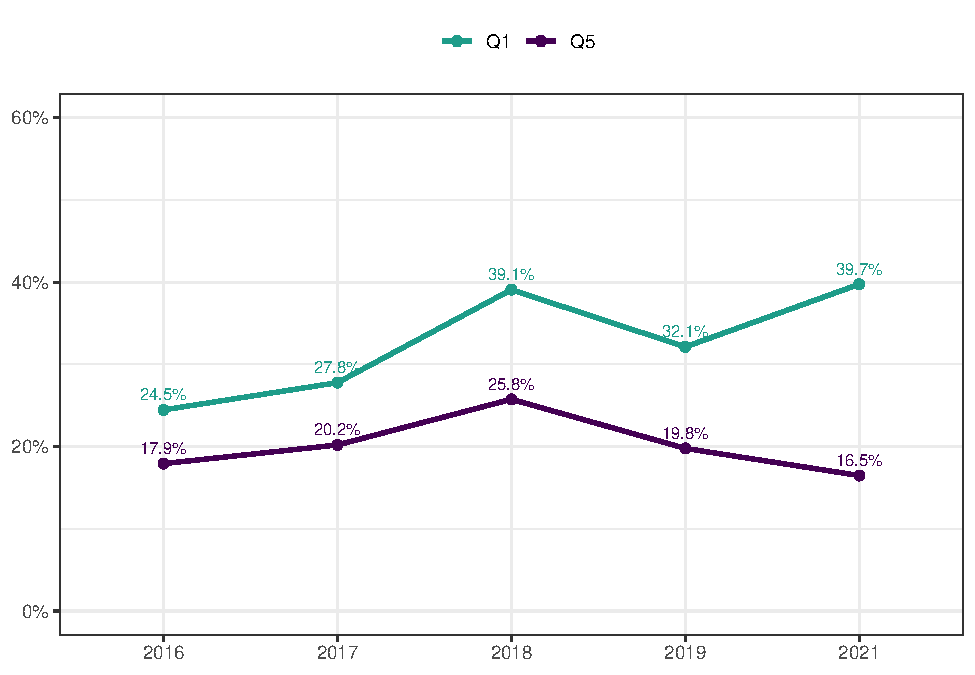
\includegraphics{reporte-elsoc_files/figure-latex/crim-quintil-1} 

}

\caption{¿Con qué frecuencia se han producido crímenes (riñas, robos y tráfico de drogas) en su barrio?, según ola del estudio y quintil de ingreso. Porcentaje de experiencias de criminalidad "Siempre" o "Muchas veces".}\label{fig:crim-quintil}
\end{figure}

\hypertarget{cartografuxeda-de-la-criminalidad-barrial}{%
\subsection{Cartografía de la criminalidad barrial}\label{cartografuxeda-de-la-criminalidad-barrial}}

\begin{Shaded}
\begin{Highlighting}[]
\NormalTok{elsoc\_comuna\_rm }\OtherTok{\textless{}{-}}\NormalTok{ elsoc\_long\_2016\_2021 }\SpecialCharTok{\%\textgreater{}\%} 
  \FunctionTok{filter}\NormalTok{(tipo\_atricion }\SpecialCharTok{==} \DecValTok{1} \SpecialCharTok{\&}\NormalTok{ muestra }\SpecialCharTok{==} \DecValTok{1} \SpecialCharTok{\&}\NormalTok{ ola }\SpecialCharTok{==} \DecValTok{5} \SpecialCharTok{\&}\NormalTok{ region\_cod }\SpecialCharTok{==} \DecValTok{13} \SpecialCharTok{\&} \SpecialCharTok{!}\NormalTok{t09\_01 }\SpecialCharTok{\%in\%} \FunctionTok{c}\NormalTok{(}\SpecialCharTok{{-}}\DecValTok{888}\NormalTok{, }\SpecialCharTok{{-}}\DecValTok{999}\NormalTok{) }\SpecialCharTok{\&}
           \SpecialCharTok{!}\NormalTok{t09\_02 }\SpecialCharTok{\%in\%} \FunctionTok{c}\NormalTok{(}\SpecialCharTok{{-}}\DecValTok{888}\NormalTok{, }\SpecialCharTok{{-}}\DecValTok{999}\NormalTok{) }\SpecialCharTok{\&} \SpecialCharTok{!}\NormalTok{t09\_03 }\SpecialCharTok{\%in\%} \FunctionTok{c}\NormalTok{(}\SpecialCharTok{{-}}\DecValTok{888}\NormalTok{, }\SpecialCharTok{{-}}\DecValTok{999}\NormalTok{)) }\SpecialCharTok{\%\textgreater{}\%} 
  \FunctionTok{mutate}\NormalTok{(}\AttributeTok{barrio\_crim =}\NormalTok{ (t09\_01 }\SpecialCharTok{+}\NormalTok{ t09\_02 }\SpecialCharTok{+}\NormalTok{ t09\_03)}\SpecialCharTok{/}\DecValTok{3}\NormalTok{) }\SpecialCharTok{\%\textgreater{}\%}
\NormalTok{  sjlabelled}\SpecialCharTok{::}\FunctionTok{as\_label}\NormalTok{(ola) }\SpecialCharTok{\%\textgreater{}\%} 
  \FunctionTok{group\_by}\NormalTok{(comuna, comuna\_cod) }\SpecialCharTok{\%\textgreater{}\%} 
  \FunctionTok{summarise}\NormalTok{(}\AttributeTok{m\_crim =} \FunctionTok{weighted.mean}\NormalTok{(barrio\_crim, ponderador02, }\AttributeTok{na.rm =}\NormalTok{ T),}
            \AttributeTok{sd\_crim =} \FunctionTok{sd}\NormalTok{(barrio\_crim, }\AttributeTok{na.rm =}\NormalTok{ T),}
            \AttributeTok{n =} \FunctionTok{n}\NormalTok{())}

\NormalTok{comunas\_rm }\OtherTok{\textless{}{-}}\NormalTok{ chilemapas}\SpecialCharTok{::}\NormalTok{mapa\_zonas }\SpecialCharTok{\%\textgreater{}\%} 
  \FunctionTok{filter}\NormalTok{(codigo\_region}\SpecialCharTok{==}\DecValTok{13} \SpecialCharTok{\&}\NormalTok{ codigo\_provincia }\SpecialCharTok{==} \StringTok{\textquotesingle{}131\textquotesingle{}}\NormalTok{) }\SpecialCharTok{\%\textgreater{}\%} 
  \FunctionTok{st\_as\_sf}\NormalTok{(.) }\SpecialCharTok{\%\textgreater{}\%} 
  \FunctionTok{group\_by}\NormalTok{(codigo\_comuna) }\SpecialCharTok{\%\textgreater{}\%} 
  \FunctionTok{summarise}\NormalTok{()}

\NormalTok{comunas\_rm }\OtherTok{\textless{}{-}} \FunctionTok{merge}\NormalTok{(comunas\_rm, }
\NormalTok{                    elsoc\_comuna\_rm, }
                    \AttributeTok{by.x =} \StringTok{"codigo\_comuna"}\NormalTok{, }\AttributeTok{by.y =} \StringTok{"comuna\_cod"}\NormalTok{,}
                    \AttributeTok{all.x =} \ConstantTok{TRUE}\NormalTok{,}
                    \AttributeTok{sort=}\NormalTok{F)}

\CommentTok{\#comunas\_rm \textless{}{-} comunas\_rm \%\textgreater{}\% drop\_na() \#en caso de quitar comunas con NA}

\NormalTok{g.crimi.rm }\OtherTok{\textless{}{-}} 
  \FunctionTok{ggplot}\NormalTok{(comunas\_rm) }\SpecialCharTok{+} 
  \FunctionTok{geom\_sf}\NormalTok{(}\FunctionTok{aes}\NormalTok{(}\AttributeTok{fill =}\NormalTok{ m\_crim, }\AttributeTok{geometry =}\NormalTok{ geometry)) }\SpecialCharTok{+}
  \FunctionTok{labs}\NormalTok{(}\AttributeTok{y =} \ConstantTok{NULL}\NormalTok{, }\AttributeTok{x =} \ConstantTok{NULL}\NormalTok{, }\AttributeTok{fill =} \StringTok{"Criminalidad barrial}\SpecialCharTok{\textbackslash{}n}\StringTok{promedio por comuna"}\NormalTok{) }\SpecialCharTok{+}
  \FunctionTok{scale\_fill\_viridis\_c}\NormalTok{(}\AttributeTok{begin =}\NormalTok{ .}\DecValTok{11}\NormalTok{, }\AttributeTok{end =}\NormalTok{ .}\DecValTok{88}\NormalTok{, }\AttributeTok{direction =} \SpecialCharTok{{-}}\DecValTok{1}\NormalTok{, }\AttributeTok{option =} \StringTok{\textquotesingle{}viridis\textquotesingle{}}\NormalTok{) }\SpecialCharTok{+}
  \FunctionTok{theme\_bw}\NormalTok{() }
\NormalTok{g.crimi.rm}
\end{Highlighting}
\end{Shaded}

\begin{figure}

{\centering \includegraphics{reporte-elsoc_files/figure-latex/crimi-comuna-1} 

}

\caption{Frecuencia promedio de percepción de crímenes (riñas, robos y tráfico de drogas) en el barrio, según comuna de residencia en la región metropolitana (2021).}\label{fig:crimi-comuna}
\end{figure}

\begin{Shaded}
\begin{Highlighting}[]
\NormalTok{elsoc\_region }\OtherTok{\textless{}{-}}\NormalTok{ elsoc\_long\_2016\_2021 }\SpecialCharTok{\%\textgreater{}\%} 
  \FunctionTok{filter}\NormalTok{(tipo\_atricion }\SpecialCharTok{==} \DecValTok{1} \SpecialCharTok{\&}\NormalTok{ muestra }\SpecialCharTok{==} \DecValTok{1} \SpecialCharTok{\&}\NormalTok{ ola }\SpecialCharTok{==} \DecValTok{5} \SpecialCharTok{\&} \SpecialCharTok{!}\NormalTok{t09\_01 }\SpecialCharTok{\%in\%} \FunctionTok{c}\NormalTok{(}\SpecialCharTok{{-}}\DecValTok{888}\NormalTok{, }\SpecialCharTok{{-}}\DecValTok{999}\NormalTok{) }\SpecialCharTok{\&}
           \SpecialCharTok{!}\NormalTok{t09\_02 }\SpecialCharTok{\%in\%} \FunctionTok{c}\NormalTok{(}\SpecialCharTok{{-}}\DecValTok{888}\NormalTok{, }\SpecialCharTok{{-}}\DecValTok{999}\NormalTok{) }\SpecialCharTok{\&} \SpecialCharTok{!}\NormalTok{t09\_03 }\SpecialCharTok{\%in\%} \FunctionTok{c}\NormalTok{(}\SpecialCharTok{{-}}\DecValTok{888}\NormalTok{, }\SpecialCharTok{{-}}\DecValTok{999}\NormalTok{)) }\SpecialCharTok{\%\textgreater{}\%} 
  \FunctionTok{mutate}\NormalTok{(}\AttributeTok{barrio\_crim =}\NormalTok{ (t09\_01 }\SpecialCharTok{+}\NormalTok{ t09\_02 }\SpecialCharTok{+}\NormalTok{ t09\_03)}\SpecialCharTok{/}\DecValTok{3}\NormalTok{) }\SpecialCharTok{\%\textgreater{}\%}
\NormalTok{  sjlabelled}\SpecialCharTok{::}\FunctionTok{as\_label}\NormalTok{(ola) }\SpecialCharTok{\%\textgreater{}\%} 
  \FunctionTok{group\_by}\NormalTok{(region, region\_cod) }\SpecialCharTok{\%\textgreater{}\%} 
  \FunctionTok{summarise}\NormalTok{(}\AttributeTok{m\_crim =} \FunctionTok{weighted.mean}\NormalTok{(barrio\_crim, ponderador02, }\AttributeTok{na.rm =}\NormalTok{ T),}
            \AttributeTok{sd\_crim =} \FunctionTok{sd}\NormalTok{(barrio\_crim, }\AttributeTok{na.rm =}\NormalTok{ T),}
            \AttributeTok{n =} \FunctionTok{n}\NormalTok{())}

\NormalTok{elsoc\_region}\SpecialCharTok{$}\NormalTok{region\_cod }\OtherTok{\textless{}{-}} \FunctionTok{factor}\NormalTok{(elsoc\_region}\SpecialCharTok{$}\NormalTok{region\_cod,}
                                  \AttributeTok{labels =} \FunctionTok{c}\NormalTok{(}\StringTok{\textquotesingle{}01\textquotesingle{}}\NormalTok{,}\StringTok{\textquotesingle{}02\textquotesingle{}}\NormalTok{,}\StringTok{\textquotesingle{}03\textquotesingle{}}\NormalTok{,}\StringTok{\textquotesingle{}04\textquotesingle{}}\NormalTok{,}\StringTok{\textquotesingle{}05\textquotesingle{}}\NormalTok{,}\StringTok{\textquotesingle{}06\textquotesingle{}}\NormalTok{,}\StringTok{\textquotesingle{}07\textquotesingle{}}\NormalTok{,}\StringTok{\textquotesingle{}08\textquotesingle{}}\NormalTok{,}
                                            \StringTok{\textquotesingle{}09\textquotesingle{}}\NormalTok{,}\StringTok{\textquotesingle{}10\textquotesingle{}}\NormalTok{,}\StringTok{\textquotesingle{}11\textquotesingle{}}\NormalTok{,}\StringTok{\textquotesingle{}13\textquotesingle{}}\NormalTok{,}\StringTok{\textquotesingle{}14\textquotesingle{}}\NormalTok{,}\StringTok{\textquotesingle{}15\textquotesingle{}}\NormalTok{,}\StringTok{\textquotesingle{}16\textquotesingle{}}\NormalTok{))}

\NormalTok{regiones }\OtherTok{\textless{}{-}} \FunctionTok{generar\_regiones}\NormalTok{()}
\NormalTok{regiones }\OtherTok{\textless{}{-}} \FunctionTok{merge}\NormalTok{(regiones,elsoc\_region, }\AttributeTok{by.x=}\StringTok{"codigo\_region"}\NormalTok{,}\AttributeTok{by.y=}\StringTok{"region\_cod"}\NormalTok{,}\AttributeTok{all.x=}\ConstantTok{TRUE}\NormalTok{,}\AttributeTok{sort=}\NormalTok{F)}

\CommentTok{\#para intentar hacer facet\_wrap}
\CommentTok{\#regiones$mitad \textless{}{-} c(\textquotesingle{}1\textquotesingle{},\textquotesingle{}1\textquotesingle{},\textquotesingle{}1\textquotesingle{},\textquotesingle{}1\textquotesingle{},\textquotesingle{}1\textquotesingle{},\textquotesingle{}1\textquotesingle{},\textquotesingle{}1\textquotesingle{},\textquotesingle{}2\textquotesingle{},\textquotesingle{}2\textquotesingle{},\textquotesingle{}2\textquotesingle{},\textquotesingle{}2\textquotesingle{},\textquotesingle{}1\textquotesingle{},\textquotesingle{}2\textquotesingle{},\textquotesingle{}1\textquotesingle{},\textquotesingle{}2\textquotesingle{},\textquotesingle{}2\textquotesingle{})}

\NormalTok{regiones}\SpecialCharTok{$}\NormalTok{region[}\FunctionTok{is.na}\NormalTok{(regiones}\SpecialCharTok{$}\NormalTok{region)] }\OtherTok{\textless{}{-}} \StringTok{\textquotesingle{}Magallanes}\SpecialCharTok{\textbackslash{}n}\StringTok{(Sin datos)\textquotesingle{}}
\NormalTok{regiones}\SpecialCharTok{$}\NormalTok{region[regiones}\SpecialCharTok{$}\NormalTok{region }\SpecialCharTok{==} \StringTok{\textquotesingle{}Metropolitana de santiago\textquotesingle{}}\NormalTok{] }\OtherTok{\textless{}{-}} \StringTok{\textquotesingle{}Metropolitana\textquotesingle{}}
\NormalTok{regiones}\SpecialCharTok{$}\NormalTok{region[regiones}\SpecialCharTok{$}\NormalTok{region }\SpecialCharTok{==} \StringTok{\textquotesingle{}Libertador general bernardo ohiggins\textquotesingle{}}\NormalTok{] }\OtherTok{\textless{}{-}} \StringTok{\textquotesingle{}Ohiggins\textquotesingle{}}
\NormalTok{regiones}\SpecialCharTok{$}\NormalTok{region[regiones}\SpecialCharTok{$}\NormalTok{region }\SpecialCharTok{==} \StringTok{\textquotesingle{}Aysen del general carlos ibannez del campo\textquotesingle{}}\NormalTok{] }\OtherTok{\textless{}{-}} \StringTok{\textquotesingle{}Aysen\textquotesingle{}}
\NormalTok{regiones}\SpecialCharTok{$}\NormalTok{region[regiones}\SpecialCharTok{$}\NormalTok{region }\SpecialCharTok{==} \StringTok{\textquotesingle{}Arica y parinacota\textquotesingle{}}\NormalTok{] }\OtherTok{\textless{}{-}} \StringTok{\textquotesingle{}Arica\textquotesingle{}}

\NormalTok{g.crim.region }\OtherTok{\textless{}{-}}\NormalTok{ regiones }\SpecialCharTok{\%\textgreater{}\%} 
  \FunctionTok{ggplot}\NormalTok{(}\FunctionTok{aes}\NormalTok{(}\AttributeTok{fill =}\NormalTok{ m\_crim, }\AttributeTok{geometry =}\NormalTok{ geometry, }\AttributeTok{label =}\NormalTok{ region)) }\SpecialCharTok{+} 
  \FunctionTok{geom\_sf}\NormalTok{() }\SpecialCharTok{+}
  \FunctionTok{coord\_sf}\NormalTok{(}\AttributeTok{xlim =} \FunctionTok{c}\NormalTok{(}\SpecialCharTok{{-}}\DecValTok{100}\NormalTok{, }\SpecialCharTok{{-}}\DecValTok{65}\NormalTok{)) }\SpecialCharTok{+}
  \FunctionTok{labs}\NormalTok{(}\AttributeTok{y =} \ConstantTok{NULL}\NormalTok{, }\AttributeTok{x =} \ConstantTok{NULL}\NormalTok{, }\AttributeTok{fill =} \StringTok{"Criminalidad barrial}\SpecialCharTok{\textbackslash{}n}\StringTok{promedio por región"}\NormalTok{) }\SpecialCharTok{+}
  \FunctionTok{scale\_fill\_viridis\_c}\NormalTok{(}\AttributeTok{begin =}\NormalTok{ .}\DecValTok{11}\NormalTok{, }\AttributeTok{end =}\NormalTok{ .}\DecValTok{88}\NormalTok{, }\AttributeTok{direction =} \SpecialCharTok{{-}}\DecValTok{1}\NormalTok{, }\AttributeTok{option =} \StringTok{\textquotesingle{}viridis\textquotesingle{}}\NormalTok{, }\AttributeTok{na.value =} \StringTok{\textquotesingle{}white\textquotesingle{}}\NormalTok{) }\SpecialCharTok{+}
\NormalTok{  ggrepel}\SpecialCharTok{::}\FunctionTok{geom\_text\_repel}\NormalTok{(}\AttributeTok{stat =} \StringTok{"sf\_coordinates"}\NormalTok{, }\AttributeTok{min.segment.length =} \DecValTok{0}\NormalTok{,}
                           \AttributeTok{colour =} \StringTok{"black"}\NormalTok{, }\AttributeTok{segment.colour =} \StringTok{"black"}\NormalTok{,}
                           \AttributeTok{direction =} \StringTok{"y"}\NormalTok{, }\AttributeTok{hjust =} \FloatTok{2.5}\NormalTok{, }\AttributeTok{size =} \DecValTok{3}\NormalTok{) }\SpecialCharTok{+}
\NormalTok{  ggspatial}\SpecialCharTok{::}\FunctionTok{annotation\_north\_arrow}\NormalTok{(}\FunctionTok{aes}\NormalTok{(}\AttributeTok{which\_north =} \StringTok{"true"}\NormalTok{, }\AttributeTok{location =} \StringTok{"bl"}\NormalTok{), }\AttributeTok{pad\_y =} \FunctionTok{unit}\NormalTok{(}\FloatTok{0.8}\NormalTok{, }\StringTok{"cm"}\NormalTok{)) }\SpecialCharTok{+}
\NormalTok{  ggspatial}\SpecialCharTok{::}\FunctionTok{annotation\_scale}\NormalTok{(}\FunctionTok{aes}\NormalTok{(}\AttributeTok{location =} \StringTok{"bl"}\NormalTok{, }\AttributeTok{style =} \StringTok{"bar"}\NormalTok{)) }\SpecialCharTok{+}
  \FunctionTok{theme\_bw}\NormalTok{()}
\NormalTok{g.crim.region}
\end{Highlighting}
\end{Shaded}

\begin{figure}

{\centering \includegraphics{reporte-elsoc_files/figure-latex/confli-region-1} 

}

\caption{Frecuencia promedio de percepción de crímenes (riñas, robos y tráfico de drogas) en el barrio, según región de Chile (2021)}\label{fig:confli-region}
\end{figure}

\hypertarget{distanciamiento-y-comportamiento-prosocial-en-pandemia}{%
\chapter{Distanciamiento y comportamiento prosocial en pandemia}\label{distanciamiento-y-comportamiento-prosocial-en-pandemia}}

\hypertarget{distanciamiento-social}{%
\section{Distanciamiento social}\label{distanciamiento-social}}

\begin{Shaded}
\begin{Highlighting}[]
\NormalTok{datos.}\FloatTok{9.1} \OtherTok{\textless{}{-}}\NormalTok{ elsoc\_long\_2016\_2021 }\SpecialCharTok{\%\textgreater{}\%} 
  \FunctionTok{filter}\NormalTok{(tipo\_atricion }\SpecialCharTok{==} \DecValTok{1} \SpecialCharTok{\&}\NormalTok{ muestra }\SpecialCharTok{==} \DecValTok{1} \SpecialCharTok{\&}\NormalTok{ ola }\SpecialCharTok{\%in\%} \FunctionTok{c}\NormalTok{(}\DecValTok{5}\NormalTok{) }\SpecialCharTok{\&} \SpecialCharTok{!}\NormalTok{c48 }\SpecialCharTok{\%in\%} \FunctionTok{c}\NormalTok{(}\SpecialCharTok{{-}}\DecValTok{888}\NormalTok{, }\SpecialCharTok{{-}}\DecValTok{999}\NormalTok{)) }\SpecialCharTok{\%\textgreater{}\%} 
  \FunctionTok{mutate}\NormalTok{(}\AttributeTok{dis\_soc =} \FunctionTok{factor}\NormalTok{(car}\SpecialCharTok{::}\FunctionTok{recode}\NormalTok{(c48, }\StringTok{"c(1,2) = 1; c(3) = 2; c(4,5) = 3"}\NormalTok{),}
                               \AttributeTok{levels =} \FunctionTok{c}\NormalTok{(}\DecValTok{1}\NormalTok{,}\DecValTok{2}\NormalTok{,}\DecValTok{3}\NormalTok{),}
                               \AttributeTok{labels=} \FunctionTok{c}\NormalTok{(}\StringTok{"Nunca o casi nunca"}\NormalTok{, }\StringTok{"A veces"}\NormalTok{,}
                                         \StringTok{"Frecuentemente o}\SpecialCharTok{\textbackslash{}n}\StringTok{muy frecuentemente"}\NormalTok{))) }\SpecialCharTok{\%\textgreater{}\%}
  \FunctionTok{prop}\NormalTok{(}\AttributeTok{x =}\NormalTok{ dis\_soc, }\AttributeTok{na.rm =} \ConstantTok{TRUE}\NormalTok{)}

\NormalTok{g9}\FloatTok{.1} \OtherTok{\textless{}{-}}\NormalTok{ datos.}\FloatTok{9.1} \SpecialCharTok{\%\textgreater{}\%} 
  \FunctionTok{ggplot}\NormalTok{(}\FunctionTok{aes}\NormalTok{(}\AttributeTok{y =}\NormalTok{ prop, }\AttributeTok{x =}\NormalTok{ dis\_soc, }\AttributeTok{fill =}\NormalTok{ dis\_soc, }
             \AttributeTok{label =} \FunctionTok{as.character}\NormalTok{(scales}\SpecialCharTok{::}\FunctionTok{percent}\NormalTok{(prop, }\AttributeTok{accuracy =}\NormalTok{ .}\DecValTok{1}\NormalTok{)))) }\SpecialCharTok{+}
  \FunctionTok{theme\_bw}\NormalTok{() }\SpecialCharTok{+} 
  \FunctionTok{geom\_col}\NormalTok{(}\AttributeTok{position =} \StringTok{\textquotesingle{}Dodge\textquotesingle{}}\NormalTok{) }\SpecialCharTok{+}
  \FunctionTok{scale\_y\_continuous}\NormalTok{(}\AttributeTok{labels =}\NormalTok{ scales}\SpecialCharTok{::}\NormalTok{percent,}
                      \AttributeTok{limits =} \FunctionTok{c}\NormalTok{(}\DecValTok{0}\NormalTok{, }\DecValTok{1}\NormalTok{)) }\SpecialCharTok{+}
  \FunctionTok{ylab}\NormalTok{(}\AttributeTok{label =} \ConstantTok{NULL}\NormalTok{) }\SpecialCharTok{+}
  \FunctionTok{xlab}\NormalTok{(}\AttributeTok{label =} \ConstantTok{NULL}\NormalTok{) }\SpecialCharTok{+}
  \FunctionTok{scale\_fill\_viridis\_d}\NormalTok{(}\AttributeTok{begin =} \DecValTok{0}\NormalTok{, }\AttributeTok{end =}\NormalTok{ .}\DecValTok{85}\NormalTok{, }\AttributeTok{direction =} \SpecialCharTok{{-}}\DecValTok{1}\NormalTok{, }\AttributeTok{option =} \StringTok{\textquotesingle{}viridis\textquotesingle{}}\NormalTok{) }\SpecialCharTok{+}
  \FunctionTok{geom\_text}\NormalTok{(}\AttributeTok{vjust =} \SpecialCharTok{{-}}\FloatTok{0.8}\NormalTok{,}
            \AttributeTok{position =} \FunctionTok{position\_dodge}\NormalTok{(}\AttributeTok{width =}\NormalTok{ .}\DecValTok{9}\NormalTok{),}
            \AttributeTok{size=} \FloatTok{2.75}\NormalTok{) }\SpecialCharTok{+}
  \FunctionTok{theme}\NormalTok{(}\AttributeTok{legend.position =} \StringTok{\textquotesingle{}none\textquotesingle{}}\NormalTok{, }
        \AttributeTok{legend.title =} \FunctionTok{element\_blank}\NormalTok{())}
\NormalTok{g9}\FloatTok{.1}
\end{Highlighting}
\end{Shaded}

\begin{figure}

{\centering \includegraphics{reporte-elsoc_files/figure-latex/dist-total-1} 

}

\caption{¿En qué medida usted ha seguido la recomendación de quedarse en su hogar, manteniendo el aislamiento social? (2021).}\label{fig:dist-total}
\end{figure}

\begin{Shaded}
\begin{Highlighting}[]
\NormalTok{datos.}\FloatTok{9.2} \OtherTok{\textless{}{-}}\NormalTok{ elsoc\_long\_2016\_2021 }\SpecialCharTok{\%\textgreater{}\%} 
  \FunctionTok{filter}\NormalTok{(tipo\_atricion }\SpecialCharTok{==} \DecValTok{1} \SpecialCharTok{\&}\NormalTok{ muestra }\SpecialCharTok{==} \DecValTok{1} \SpecialCharTok{\&}\NormalTok{ ola }\SpecialCharTok{\%in\%} \FunctionTok{c}\NormalTok{(}\DecValTok{5}\NormalTok{) }\SpecialCharTok{\&} \SpecialCharTok{!}\NormalTok{t01 }\SpecialCharTok{\%in\%} \FunctionTok{c}\NormalTok{(}\SpecialCharTok{{-}}\DecValTok{888}\NormalTok{, }\SpecialCharTok{{-}}\DecValTok{999}\NormalTok{)) }\SpecialCharTok{\%\textgreater{}\%} 
  \FunctionTok{mutate}\NormalTok{(}\AttributeTok{dis\_soc =} \FunctionTok{factor}\NormalTok{(car}\SpecialCharTok{::}\FunctionTok{recode}\NormalTok{(c48, }\StringTok{"c(1,2) = 1; c(3) = 2; c(4,5) = 3"}\NormalTok{),}
                               \AttributeTok{levels =} \FunctionTok{c}\NormalTok{(}\DecValTok{1}\NormalTok{,}\DecValTok{2}\NormalTok{,}\DecValTok{3}\NormalTok{), }\AttributeTok{labels=} \FunctionTok{c}\NormalTok{(}\StringTok{"Nunca o casi nunca"}\NormalTok{, }\StringTok{"A veces"}\NormalTok{,}
                                         \StringTok{"Frecuentemente o}\SpecialCharTok{\textbackslash{}n}\StringTok{muy frecuentemente"}\NormalTok{)),}
         \AttributeTok{m30 =} \FunctionTok{as.numeric}\NormalTok{(car}\SpecialCharTok{::}\FunctionTok{recode}\NormalTok{(m30,}\StringTok{"1=110000;2=251000;3=305000;4=355000;5=400000;6=445000;}
\StringTok{                                           7=490000;8=535000;9=585000;10=640000;11=700000;12=765000;}
\StringTok{                                           13=845000;14=935000;15=1040000;16=1180000;17=1375000;}
\StringTok{                                           18=1670000;19=2275000;20=2700000;NA=NA"}\NormalTok{)),}
         \AttributeTok{m29\_imp =} \FunctionTok{ifelse}\NormalTok{(}\SpecialCharTok{!}\FunctionTok{is.na}\NormalTok{(m29),m29, m30),}
         \AttributeTok{n\_hogar =} \FunctionTok{case\_when}\NormalTok{(ola }\SpecialCharTok{==} \DecValTok{1} \SpecialCharTok{\textasciitilde{}}\NormalTok{ nhogar1, ola }\SpecialCharTok{==} \DecValTok{2} \SpecialCharTok{\textasciitilde{}}\NormalTok{ m46\_nhogar,}
\NormalTok{                             ola }\SpecialCharTok{==} \DecValTok{3} \SpecialCharTok{\textasciitilde{}}\NormalTok{ m54, ola }\SpecialCharTok{==} \DecValTok{4} \SpecialCharTok{\textasciitilde{}}\NormalTok{ m54, ola }\SpecialCharTok{==} \DecValTok{5} \SpecialCharTok{\textasciitilde{}}\NormalTok{ m54)) }\SpecialCharTok{\%\textgreater{}\%}
  \FunctionTok{mutate}\NormalTok{(}\AttributeTok{ing\_pc =}\NormalTok{ (m29\_imp}\SpecialCharTok{/}\NormalTok{n\_hogar)) }\SpecialCharTok{\%\textgreater{}\%}
\NormalTok{  sjlabelled}\SpecialCharTok{::}\FunctionTok{as\_label}\NormalTok{(ola) }\SpecialCharTok{\%\textgreater{}\%} 
  \FunctionTok{group\_by}\NormalTok{(ola) }\SpecialCharTok{\%\textgreater{}\%} 
  \FunctionTok{mutate}\NormalTok{(}\AttributeTok{quintil =} \FunctionTok{factor}\NormalTok{(}\FunctionTok{ntile}\NormalTok{(}\SpecialCharTok{{-}}\FunctionTok{desc}\NormalTok{(ing\_pc), }\DecValTok{5}\NormalTok{), }\AttributeTok{levels =} \FunctionTok{c}\NormalTok{(}\DecValTok{1}\NormalTok{,}\DecValTok{2}\NormalTok{,}\DecValTok{3}\NormalTok{,}\DecValTok{4}\NormalTok{,}\DecValTok{5}\NormalTok{),}
         \AttributeTok{labels =} \FunctionTok{c}\NormalTok{(}\StringTok{\textquotesingle{}Q1\textquotesingle{}}\NormalTok{, }\StringTok{\textquotesingle{}Q2\textquotesingle{}}\NormalTok{, }\StringTok{\textquotesingle{}Q3\textquotesingle{}}\NormalTok{, }\StringTok{\textquotesingle{}Q4\textquotesingle{}}\NormalTok{, }\StringTok{\textquotesingle{}Q5\textquotesingle{}}\NormalTok{))) }\SpecialCharTok{\%\textgreater{}\%} 
  \FunctionTok{prop}\NormalTok{(}\AttributeTok{x =}\NormalTok{ dis\_soc, }\AttributeTok{by =} \FunctionTok{c}\NormalTok{(ola, quintil), }\AttributeTok{na.rm =} \ConstantTok{TRUE}\NormalTok{) }\SpecialCharTok{\%\textgreater{}\%} 
  \FunctionTok{filter}\NormalTok{(dis\_soc }\SpecialCharTok{==} \StringTok{"Frecuentemente o}\SpecialCharTok{\textbackslash{}n}\StringTok{muy frecuentemente"}\NormalTok{)}

\NormalTok{g9}\FloatTok{.2} \OtherTok{\textless{}{-}} 
\NormalTok{  datos.}\FloatTok{9.2} \SpecialCharTok{\%\textgreater{}\%} 
  \FunctionTok{ggplot}\NormalTok{(}\FunctionTok{aes}\NormalTok{(}\AttributeTok{y =}\NormalTok{ prop, }\AttributeTok{x =}\NormalTok{ quintil, }\AttributeTok{fill =}\NormalTok{ quintil, }
             \AttributeTok{label =} \FunctionTok{as.character}\NormalTok{(scales}\SpecialCharTok{::}\FunctionTok{percent}\NormalTok{(prop, }\AttributeTok{accuracy =}\NormalTok{ .}\DecValTok{1}\NormalTok{)))) }\SpecialCharTok{+} 
  \FunctionTok{theme\_bw}\NormalTok{() }\SpecialCharTok{+} 
  \FunctionTok{geom\_col}\NormalTok{(}\AttributeTok{position =} \StringTok{\textquotesingle{}Dodge\textquotesingle{}}\NormalTok{) }\SpecialCharTok{+}
  \FunctionTok{scale\_y\_continuous}\NormalTok{(}\AttributeTok{labels =}\NormalTok{ scales}\SpecialCharTok{::}\NormalTok{percent,}
                      \AttributeTok{limits =} \FunctionTok{c}\NormalTok{(}\DecValTok{0}\NormalTok{, }\DecValTok{1}\NormalTok{)) }\SpecialCharTok{+}
  \FunctionTok{ylab}\NormalTok{(}\AttributeTok{label =} \ConstantTok{NULL}\NormalTok{) }\SpecialCharTok{+}
  \FunctionTok{xlab}\NormalTok{(}\AttributeTok{label =} \ConstantTok{NULL}\NormalTok{) }\SpecialCharTok{+}
  \FunctionTok{scale\_fill\_viridis\_d}\NormalTok{(}\AttributeTok{begin =} \DecValTok{0}\NormalTok{, }\AttributeTok{end =}\NormalTok{ .}\DecValTok{99}\NormalTok{, }\AttributeTok{direction =} \SpecialCharTok{{-}}\DecValTok{1}\NormalTok{, }\AttributeTok{option =} \StringTok{\textquotesingle{}viridis\textquotesingle{}}\NormalTok{) }\SpecialCharTok{+}
  \FunctionTok{geom\_text}\NormalTok{(}\AttributeTok{vjust =} \SpecialCharTok{{-}}\FloatTok{0.8}\NormalTok{,}
            \AttributeTok{position =} \FunctionTok{position\_dodge}\NormalTok{(}\AttributeTok{width =}\NormalTok{ .}\DecValTok{9}\NormalTok{),}
            \AttributeTok{size=} \FloatTok{2.75}\NormalTok{) }\SpecialCharTok{+} 
  \FunctionTok{theme}\NormalTok{(}\AttributeTok{legend.position =} \StringTok{\textquotesingle{}none\textquotesingle{}}\NormalTok{,}
        \AttributeTok{legend.title =} \FunctionTok{element\_blank}\NormalTok{())}
\NormalTok{g9}\FloatTok{.2}
\end{Highlighting}
\end{Shaded}

\begin{figure}

{\centering \includegraphics{reporte-elsoc_files/figure-latex/dist-quintil-1} 

}

\caption{¿En qué medida usted ha seguido la recomendación de quedarse en su hogar, manteniendo el aislamiento social? según quintil de ingreso. Suma de respuestas "Frecuente o "Muy frecuentemente" (2021).}\label{fig:dist-quintil}
\end{figure}

\begin{Shaded}
\begin{Highlighting}[]
\NormalTok{datos.}\FloatTok{9.3} \OtherTok{\textless{}{-}}\NormalTok{ elsoc\_long\_2016\_2021 }\SpecialCharTok{\%\textgreater{}\%} 
  \FunctionTok{filter}\NormalTok{(tipo\_atricion }\SpecialCharTok{==} \DecValTok{1} \SpecialCharTok{\&}\NormalTok{ muestra }\SpecialCharTok{==} \DecValTok{1} \SpecialCharTok{\&}\NormalTok{ ola }\SpecialCharTok{\%in\%} \FunctionTok{c}\NormalTok{(}\DecValTok{5}\NormalTok{) }\SpecialCharTok{\&} \SpecialCharTok{!}\NormalTok{c48 }\SpecialCharTok{\%in\%} \FunctionTok{c}\NormalTok{(}\SpecialCharTok{{-}}\DecValTok{888}\NormalTok{, }\SpecialCharTok{{-}}\DecValTok{999}\NormalTok{)) }\SpecialCharTok{\%\textgreater{}\%} 
  \FunctionTok{mutate}\NormalTok{(}\AttributeTok{dis\_soc =} \FunctionTok{factor}\NormalTok{(car}\SpecialCharTok{::}\FunctionTok{recode}\NormalTok{(c48, }\StringTok{"c(1,2) = 1; c(3) = 2; c(4,5) = 3"}\NormalTok{),}
                               \AttributeTok{levels =} \FunctionTok{c}\NormalTok{(}\DecValTok{1}\NormalTok{,}\DecValTok{2}\NormalTok{,}\DecValTok{3}\NormalTok{),}
                               \AttributeTok{labels=} \FunctionTok{c}\NormalTok{(}\StringTok{"Nunca o}\SpecialCharTok{\textbackslash{}n}\StringTok{casi nunca"}\NormalTok{, }\StringTok{"A veces"}\NormalTok{,}
                                         \StringTok{"Frecuentemente o}\SpecialCharTok{\textbackslash{}n}\StringTok{muy frecuentemente"}\NormalTok{)),}
         \AttributeTok{edadt =} \FunctionTok{factor}\NormalTok{(car}\SpecialCharTok{::}\FunctionTok{recode}\NormalTok{(m0\_edad, }\StringTok{"18:29=1; 30:49=2; 50:64=3 ;65:150=4"}\NormalTok{),}
                        \AttributeTok{levels =} \FunctionTok{c}\NormalTok{(}\DecValTok{1}\NormalTok{,}\DecValTok{2}\NormalTok{,}\DecValTok{3}\NormalTok{,}\DecValTok{4}\NormalTok{), }\AttributeTok{labels =} \FunctionTok{c}\NormalTok{(}\StringTok{\textquotesingle{}18{-}29\textquotesingle{}}\NormalTok{, }\StringTok{\textquotesingle{}30{-}49\textquotesingle{}}\NormalTok{, }\StringTok{\textquotesingle{}50{-}64\textquotesingle{}}\NormalTok{, }\StringTok{\textquotesingle{}65 o más\textquotesingle{}}\NormalTok{))) }\SpecialCharTok{\%\textgreater{}\%}
  \FunctionTok{prop}\NormalTok{(}\AttributeTok{x =}\NormalTok{ dis\_soc, }\AttributeTok{by =}\NormalTok{ edadt, }\AttributeTok{na.rm =} \ConstantTok{TRUE}\NormalTok{) }\SpecialCharTok{\%\textgreater{}\%} 
  \FunctionTok{filter}\NormalTok{(dis\_soc }\SpecialCharTok{==} \StringTok{"Frecuentemente o}\SpecialCharTok{\textbackslash{}n}\StringTok{muy frecuentemente"}\NormalTok{)}

\NormalTok{g9}\FloatTok{.3} \OtherTok{\textless{}{-}} 
\NormalTok{  datos.}\FloatTok{9.3} \SpecialCharTok{\%\textgreater{}\%} 
  \FunctionTok{ggplot}\NormalTok{(}\FunctionTok{aes}\NormalTok{(}\AttributeTok{y =}\NormalTok{ prop, }\AttributeTok{x =}\NormalTok{ edadt, }\AttributeTok{fill =}\NormalTok{ edadt, }
             \AttributeTok{label =} \FunctionTok{as.character}\NormalTok{(scales}\SpecialCharTok{::}\FunctionTok{percent}\NormalTok{(prop, }\AttributeTok{accuracy =}\NormalTok{ .}\DecValTok{1}\NormalTok{)))) }\SpecialCharTok{+} 
  \FunctionTok{theme\_bw}\NormalTok{() }\SpecialCharTok{+} 
  \FunctionTok{geom\_col}\NormalTok{(}\AttributeTok{position =} \StringTok{\textquotesingle{}Dodge\textquotesingle{}}\NormalTok{) }\SpecialCharTok{+}
  \FunctionTok{scale\_y\_continuous}\NormalTok{(}\AttributeTok{labels =}\NormalTok{ scales}\SpecialCharTok{::}\NormalTok{percent,}
                      \AttributeTok{limits =} \FunctionTok{c}\NormalTok{(}\DecValTok{0}\NormalTok{, }\DecValTok{1}\NormalTok{)) }\SpecialCharTok{+}
  \FunctionTok{ylab}\NormalTok{(}\AttributeTok{label =} \ConstantTok{NULL}\NormalTok{) }\SpecialCharTok{+}
  \FunctionTok{xlab}\NormalTok{(}\AttributeTok{label =} \ConstantTok{NULL}\NormalTok{) }\SpecialCharTok{+}
  \FunctionTok{scale\_fill\_viridis\_d}\NormalTok{(}\AttributeTok{begin =} \DecValTok{0}\NormalTok{, }\AttributeTok{end =}\NormalTok{ .}\DecValTok{99}\NormalTok{, }\AttributeTok{direction =} \SpecialCharTok{{-}}\DecValTok{1}\NormalTok{, }\AttributeTok{option =} \StringTok{\textquotesingle{}viridis\textquotesingle{}}\NormalTok{) }\SpecialCharTok{+}
  \FunctionTok{geom\_text}\NormalTok{(}\AttributeTok{vjust =} \SpecialCharTok{{-}}\FloatTok{0.8}\NormalTok{,}
            \AttributeTok{position =} \FunctionTok{position\_dodge}\NormalTok{(}\AttributeTok{width =}\NormalTok{ .}\DecValTok{9}\NormalTok{),}
            \AttributeTok{size=} \FloatTok{2.75}\NormalTok{) }\SpecialCharTok{+} 
  \FunctionTok{theme}\NormalTok{(}\AttributeTok{legend.position =} \StringTok{\textquotesingle{}none\textquotesingle{}}\NormalTok{,}
        \AttributeTok{legend.title =} \FunctionTok{element\_blank}\NormalTok{())}
\NormalTok{g9}\FloatTok{.3}
\end{Highlighting}
\end{Shaded}

\begin{figure}

{\centering \includegraphics{reporte-elsoc_files/figure-latex/dist-edad-1} 

}

\caption{¿En qué medida usted ha seguido la recomendación de quedarse en su hogar, manteniendo el aislamiento social? según edad. Suma de respuestas "Frecuente o "Muy frecuentemente" (2021).}\label{fig:dist-edad}
\end{figure}

\begin{Shaded}
\begin{Highlighting}[]
\NormalTok{datos.}\FloatTok{9.4} \OtherTok{\textless{}{-}}\NormalTok{ elsoc\_long\_2016\_2021 }\SpecialCharTok{\%\textgreater{}\%} 
  \FunctionTok{filter}\NormalTok{(tipo\_atricion }\SpecialCharTok{==} \DecValTok{1} \SpecialCharTok{\&}\NormalTok{ muestra }\SpecialCharTok{==} \DecValTok{1} \SpecialCharTok{\&}\NormalTok{ ola }\SpecialCharTok{\%in\%} \FunctionTok{c}\NormalTok{(}\DecValTok{5}\NormalTok{) }\SpecialCharTok{\&} \SpecialCharTok{!}\NormalTok{c48 }\SpecialCharTok{\%in\%} \FunctionTok{c}\NormalTok{(}\SpecialCharTok{{-}}\DecValTok{888}\NormalTok{, }\SpecialCharTok{{-}}\DecValTok{999}\NormalTok{)) }\SpecialCharTok{\%\textgreater{}\%} 
  \FunctionTok{mutate}\NormalTok{(}\AttributeTok{dis\_soc =} \FunctionTok{factor}\NormalTok{(car}\SpecialCharTok{::}\FunctionTok{recode}\NormalTok{(c48, }\StringTok{"c(1,2) = 1; c(3) = 2; c(4,5) = 3"}\NormalTok{),}
                               \AttributeTok{levels =} \FunctionTok{c}\NormalTok{(}\DecValTok{1}\NormalTok{,}\DecValTok{2}\NormalTok{,}\DecValTok{3}\NormalTok{),}
                               \AttributeTok{labels=} \FunctionTok{c}\NormalTok{(}\StringTok{"Nunca o}\SpecialCharTok{\textbackslash{}n}\StringTok{casi nunca"}\NormalTok{, }\StringTok{"A veces"}\NormalTok{,}
                                         \StringTok{"Frecuentemente o}\SpecialCharTok{\textbackslash{}n}\StringTok{muy frecuentemente"}\NormalTok{)),}
         \AttributeTok{estrato =} \FunctionTok{factor}\NormalTok{(estrato, }\AttributeTok{levels =} \FunctionTok{c}\NormalTok{(}\DecValTok{1}\NormalTok{,}\DecValTok{2}\NormalTok{,}\DecValTok{3}\NormalTok{,}\DecValTok{4}\NormalTok{,}\DecValTok{5}\NormalTok{,}\DecValTok{6}\NormalTok{),}
                          \AttributeTok{labels =} \FunctionTok{c}\NormalTok{(}\StringTok{\textquotesingle{}Gran}\SpecialCharTok{\textbackslash{}n}\StringTok{Santiago\textquotesingle{}}\NormalTok{, }\StringTok{\textquotesingle{}Gran}\SpecialCharTok{\textbackslash{}n}\StringTok{Valparaíso\textquotesingle{}}\NormalTok{, }\StringTok{\textquotesingle{}Gran}\SpecialCharTok{\textbackslash{}n}\StringTok{Concepción\textquotesingle{}}\NormalTok{,}
                                     \StringTok{\textquotesingle{}Ciudades}\SpecialCharTok{\textbackslash{}n}\StringTok{grandes\textquotesingle{}}\NormalTok{, }\StringTok{\textquotesingle{}Ciudades}\SpecialCharTok{\textbackslash{}n}\StringTok{medianas\textquotesingle{}}\NormalTok{, }\StringTok{\textquotesingle{}Ciudades}\SpecialCharTok{\textbackslash{}n}\StringTok{pequeñas\textquotesingle{}}\NormalTok{))) }\SpecialCharTok{\%\textgreater{}\%}
  \FunctionTok{prop}\NormalTok{(}\AttributeTok{x =}\NormalTok{ dis\_soc, }\AttributeTok{by =}\NormalTok{ estrato, }\AttributeTok{na.rm =} \ConstantTok{TRUE}\NormalTok{)}

\NormalTok{g9}\FloatTok{.4} \OtherTok{\textless{}{-}}\NormalTok{ datos.}\FloatTok{9.4} \SpecialCharTok{\%\textgreater{}\%}
  \FunctionTok{ggplot}\NormalTok{(}\FunctionTok{aes}\NormalTok{(}\AttributeTok{y =}\NormalTok{ prop, }\AttributeTok{x =}\NormalTok{ estrato, }\AttributeTok{fill =}\NormalTok{ dis\_soc, }
             \AttributeTok{label =} \FunctionTok{as.character}\NormalTok{(scales}\SpecialCharTok{::}\FunctionTok{percent}\NormalTok{(prop, }\AttributeTok{accuracy =}\NormalTok{ .}\DecValTok{1}\NormalTok{)))) }\SpecialCharTok{+} 
  \FunctionTok{theme\_bw}\NormalTok{() }\SpecialCharTok{+} 
  \FunctionTok{geom\_col}\NormalTok{(}\AttributeTok{position =} \StringTok{\textquotesingle{}Stack\textquotesingle{}}\NormalTok{) }\SpecialCharTok{+}
  \FunctionTok{ylab}\NormalTok{(}\AttributeTok{label =} \ConstantTok{NULL}\NormalTok{) }\SpecialCharTok{+}
  \FunctionTok{xlab}\NormalTok{(}\AttributeTok{label =} \ConstantTok{NULL}\NormalTok{) }\SpecialCharTok{+}
  \FunctionTok{scale\_fill\_viridis\_d}\NormalTok{(}\AttributeTok{begin =} \DecValTok{0}\NormalTok{, }\AttributeTok{end =}\NormalTok{ .}\DecValTok{99}\NormalTok{, }\AttributeTok{direction =} \SpecialCharTok{{-}}\DecValTok{1}\NormalTok{, }\AttributeTok{option =} \StringTok{\textquotesingle{}viridis\textquotesingle{}}\NormalTok{) }\SpecialCharTok{+}
  \FunctionTok{geom\_text}\NormalTok{(}\AttributeTok{position =} \FunctionTok{position\_stack}\NormalTok{(}\AttributeTok{vjust =}\NormalTok{ .}\DecValTok{5}\NormalTok{),}
            \AttributeTok{size=} \FloatTok{2.75}\NormalTok{, }\AttributeTok{color =} \FunctionTok{rep.int}\NormalTok{(}\FunctionTok{c}\NormalTok{( }\StringTok{\textquotesingle{}black\textquotesingle{}}\NormalTok{,}\StringTok{\textquotesingle{}black\textquotesingle{}}\NormalTok{,}\StringTok{\textquotesingle{}white\textquotesingle{}}\NormalTok{), }\DecValTok{6}\NormalTok{)) }\SpecialCharTok{+} 
  \FunctionTok{theme}\NormalTok{(}\AttributeTok{legend.position =} \StringTok{\textquotesingle{}top\textquotesingle{}}\NormalTok{,}
        \AttributeTok{legend.title =} \FunctionTok{element\_blank}\NormalTok{())}
\NormalTok{g9}\FloatTok{.4}
\end{Highlighting}
\end{Shaded}

\begin{figure}

{\centering \includegraphics{reporte-elsoc_files/figure-latex/dist-estrato-1} 

}

\caption{¿En qué medida usted ha seguido la recomendación de quedarse en su hogar, manteniendo el aislamiento social? según estrato muestral (2021).}\label{fig:dist-estrato}
\end{figure}

\begin{Shaded}
\begin{Highlighting}[]
\NormalTok{datos.}\FloatTok{9.5} \OtherTok{\textless{}{-}}\NormalTok{ elsoc\_long\_2016\_2021 }\SpecialCharTok{\%\textgreater{}\%} 
  \FunctionTok{filter}\NormalTok{(tipo\_atricion }\SpecialCharTok{==} \DecValTok{1} \SpecialCharTok{\&}\NormalTok{ muestra }\SpecialCharTok{==} \DecValTok{1} \SpecialCharTok{\&}\NormalTok{ ola }\SpecialCharTok{\%in\%} \FunctionTok{c}\NormalTok{(}\DecValTok{5}\NormalTok{) }\SpecialCharTok{\&} \SpecialCharTok{!}\NormalTok{c48 }\SpecialCharTok{\%in\%} \FunctionTok{c}\NormalTok{(}\SpecialCharTok{{-}}\DecValTok{888}\NormalTok{, }\SpecialCharTok{{-}}\DecValTok{999}\NormalTok{) }\SpecialCharTok{\&} \SpecialCharTok{!}\NormalTok{m60 }\SpecialCharTok{\%in\%} \FunctionTok{c}\NormalTok{(}\SpecialCharTok{{-}}\DecValTok{888}\NormalTok{, }\SpecialCharTok{{-}}\DecValTok{999}\NormalTok{)) }\SpecialCharTok{\%\textgreater{}\%} 
  \FunctionTok{mutate}\NormalTok{(}\AttributeTok{dis\_soc =} \FunctionTok{factor}\NormalTok{(car}\SpecialCharTok{::}\FunctionTok{recode}\NormalTok{(c48, }\StringTok{"c(1,2) = 1; c(3) = 2; c(4,5) = 3"}\NormalTok{),}
                               \AttributeTok{levels =} \FunctionTok{c}\NormalTok{(}\DecValTok{1}\NormalTok{,}\DecValTok{2}\NormalTok{,}\DecValTok{3}\NormalTok{),}
                               \AttributeTok{labels=} \FunctionTok{c}\NormalTok{(}\StringTok{"Nunca o}\SpecialCharTok{\textbackslash{}n}\StringTok{casi nunca"}\NormalTok{, }\StringTok{"A veces"}\NormalTok{,}
                                         \StringTok{"Frecuentemente o}\SpecialCharTok{\textbackslash{}n}\StringTok{muy frecuentemente"}\NormalTok{)),}
         \AttributeTok{trab\_pandemia =} \FunctionTok{factor}\NormalTok{(m60, }\AttributeTok{labels =} \FunctionTok{c}\NormalTok{(}\StringTok{\textquotesingle{}Trabajo de manera}\SpecialCharTok{\textbackslash{}n}\StringTok{completa desde el hogar\textquotesingle{}}\NormalTok{,}
                                                \StringTok{\textquotesingle{}Trabajo de manera}\SpecialCharTok{\textbackslash{}n}\StringTok{parcial desde el hogar\textquotesingle{}}\NormalTok{,}
                                                \StringTok{\textquotesingle{}Trabajo fuera}\SpecialCharTok{\textbackslash{}n}\StringTok{del hogar\textquotesingle{}}\NormalTok{))) }\SpecialCharTok{\%\textgreater{}\%}
  \FunctionTok{prop}\NormalTok{(}\AttributeTok{x =}\NormalTok{ dis\_soc, }\AttributeTok{by =}\NormalTok{ trab\_pandemia, }\AttributeTok{na.rm =} \ConstantTok{TRUE}\NormalTok{) }\SpecialCharTok{\%\textgreater{}\%} 
  \FunctionTok{filter}\NormalTok{(dis\_soc }\SpecialCharTok{==} \StringTok{"Frecuentemente o}\SpecialCharTok{\textbackslash{}n}\StringTok{muy frecuentemente"}\NormalTok{) }\SpecialCharTok{\%\textgreater{}\%} 
  \FunctionTok{drop\_na}\NormalTok{()}

\NormalTok{g9}\FloatTok{.5} \OtherTok{\textless{}{-}} 
\NormalTok{  datos.}\FloatTok{9.5} \SpecialCharTok{\%\textgreater{}\%} 
  \FunctionTok{ggplot}\NormalTok{(}\FunctionTok{aes}\NormalTok{(}\AttributeTok{y =}\NormalTok{ prop, }\AttributeTok{x =}\NormalTok{ trab\_pandemia, }\AttributeTok{fill =}\NormalTok{ trab\_pandemia, }
             \AttributeTok{label =} \FunctionTok{as.character}\NormalTok{(scales}\SpecialCharTok{::}\FunctionTok{percent}\NormalTok{(prop, }\AttributeTok{accuracy =}\NormalTok{ .}\DecValTok{1}\NormalTok{)))) }\SpecialCharTok{+} 
  \FunctionTok{theme\_bw}\NormalTok{() }\SpecialCharTok{+} 
  \FunctionTok{geom\_col}\NormalTok{(}\AttributeTok{position =} \StringTok{\textquotesingle{}Dodge\textquotesingle{}}\NormalTok{) }\SpecialCharTok{+}
  \FunctionTok{scale\_y\_continuous}\NormalTok{(}\AttributeTok{labels =}\NormalTok{ scales}\SpecialCharTok{::}\NormalTok{percent,}
                      \AttributeTok{limits =} \FunctionTok{c}\NormalTok{(}\DecValTok{0}\NormalTok{, }\DecValTok{1}\NormalTok{)) }\SpecialCharTok{+}
  \FunctionTok{ylab}\NormalTok{(}\AttributeTok{label =} \ConstantTok{NULL}\NormalTok{) }\SpecialCharTok{+}
  \FunctionTok{xlab}\NormalTok{(}\AttributeTok{label =} \ConstantTok{NULL}\NormalTok{) }\SpecialCharTok{+}
  \FunctionTok{scale\_fill\_viridis\_d}\NormalTok{(}\AttributeTok{begin =} \DecValTok{0}\NormalTok{, }\AttributeTok{end =}\NormalTok{ .}\DecValTok{99}\NormalTok{, }\AttributeTok{direction =} \SpecialCharTok{{-}}\DecValTok{1}\NormalTok{, }\AttributeTok{option =} \StringTok{\textquotesingle{}viridis\textquotesingle{}}\NormalTok{) }\SpecialCharTok{+}
  \FunctionTok{geom\_text}\NormalTok{(}\AttributeTok{vjust =} \SpecialCharTok{{-}}\FloatTok{0.8}\NormalTok{,}
            \AttributeTok{position =} \FunctionTok{position\_dodge}\NormalTok{(}\AttributeTok{width =}\NormalTok{ .}\DecValTok{9}\NormalTok{),}
            \AttributeTok{size=} \FloatTok{2.75}\NormalTok{) }\SpecialCharTok{+} 
  \FunctionTok{theme}\NormalTok{(}\AttributeTok{legend.position =} \StringTok{\textquotesingle{}none\textquotesingle{}}\NormalTok{,}
        \AttributeTok{legend.title =} \FunctionTok{element\_blank}\NormalTok{())}
\NormalTok{g9}\FloatTok{.5}
\end{Highlighting}
\end{Shaded}

\begin{figure}

{\centering \includegraphics{reporte-elsoc_files/figure-latex/dist-telet-1} 

}

\caption{¿En qué medida usted ha seguido la recomendación de quedarse en su hogar, manteniendo el aislamiento social? según tipo de trabajo en pandemia. Suma de respuestas "Frecuente o "Muy frecuentemente" (2021).}\label{fig:dist-telet}
\end{figure}

\begin{Shaded}
\begin{Highlighting}[]
\NormalTok{datos.}\FloatTok{9.6} \OtherTok{\textless{}{-}}\NormalTok{ elsoc\_long\_2016\_2021 }\SpecialCharTok{\%\textgreater{}\%} 
  \FunctionTok{filter}\NormalTok{(tipo\_atricion }\SpecialCharTok{==} \DecValTok{1} \SpecialCharTok{\&}\NormalTok{ muestra }\SpecialCharTok{==} \DecValTok{1} \SpecialCharTok{\&}\NormalTok{ ola }\SpecialCharTok{\%in\%} \FunctionTok{c}\NormalTok{(}\DecValTok{5}\NormalTok{) }\SpecialCharTok{\&} \SpecialCharTok{!}\NormalTok{c48 }\SpecialCharTok{\%in\%} \FunctionTok{c}\NormalTok{(}\SpecialCharTok{{-}}\DecValTok{888}\NormalTok{, }\SpecialCharTok{{-}}\DecValTok{999}\NormalTok{) }\SpecialCharTok{\&} \SpecialCharTok{!}\NormalTok{s31 }\SpecialCharTok{\%in\%} \FunctionTok{c}\NormalTok{(}\SpecialCharTok{{-}}\DecValTok{888}\NormalTok{, }\SpecialCharTok{{-}}\DecValTok{999}\NormalTok{)) }\SpecialCharTok{\%\textgreater{}\%} 
  \FunctionTok{mutate}\NormalTok{(}\AttributeTok{dis\_soc =} \FunctionTok{factor}\NormalTok{(car}\SpecialCharTok{::}\FunctionTok{recode}\NormalTok{(c48, }\StringTok{"c(1,2) = 1; c(3) = 2; c(4,5) = 3"}\NormalTok{),}
                               \AttributeTok{levels =} \FunctionTok{c}\NormalTok{(}\DecValTok{1}\NormalTok{,}\DecValTok{2}\NormalTok{,}\DecValTok{3}\NormalTok{),}
                               \AttributeTok{labels=} \FunctionTok{c}\NormalTok{(}\StringTok{"Nunca o}\SpecialCharTok{\textbackslash{}n}\StringTok{casi nunca"}\NormalTok{, }\StringTok{"A veces"}\NormalTok{,}
                                         \StringTok{"Frecuentemente o}\SpecialCharTok{\textbackslash{}n}\StringTok{muy frecuentemente"}\NormalTok{)),}
         \AttributeTok{covid =} \FunctionTok{factor}\NormalTok{(s31, }\AttributeTok{labels =} \FunctionTok{c}\NormalTok{(}\StringTok{\textquotesingle{}Si\textquotesingle{}}\NormalTok{,}\StringTok{\textquotesingle{}No\textquotesingle{}}\NormalTok{))) }\SpecialCharTok{\%\textgreater{}\%}
  \FunctionTok{prop}\NormalTok{(}\AttributeTok{x =}\NormalTok{ dis\_soc, }\AttributeTok{by =}\NormalTok{ covid, }\AttributeTok{na.rm =} \ConstantTok{TRUE}\NormalTok{) }\SpecialCharTok{\%\textgreater{}\%} 
  \FunctionTok{filter}\NormalTok{(dis\_soc }\SpecialCharTok{==} \StringTok{"Frecuentemente o}\SpecialCharTok{\textbackslash{}n}\StringTok{muy frecuentemente"}\NormalTok{) }\SpecialCharTok{\%\textgreater{}\%} 
  \FunctionTok{drop\_na}\NormalTok{()}

\NormalTok{g9}\FloatTok{.6} \OtherTok{\textless{}{-}} 
\NormalTok{  datos.}\FloatTok{9.6} \SpecialCharTok{\%\textgreater{}\%} 
  \FunctionTok{ggplot}\NormalTok{(}\FunctionTok{aes}\NormalTok{(}\AttributeTok{y =}\NormalTok{ prop, }\AttributeTok{x =}\NormalTok{ covid, }\AttributeTok{fill =}\NormalTok{ covid, }
             \AttributeTok{label =} \FunctionTok{as.character}\NormalTok{(scales}\SpecialCharTok{::}\FunctionTok{percent}\NormalTok{(prop, }\AttributeTok{accuracy =}\NormalTok{ .}\DecValTok{1}\NormalTok{)))) }\SpecialCharTok{+} 
  \FunctionTok{theme\_bw}\NormalTok{() }\SpecialCharTok{+} 
  \FunctionTok{geom\_col}\NormalTok{(}\AttributeTok{position =} \StringTok{\textquotesingle{}Dodge\textquotesingle{}}\NormalTok{) }\SpecialCharTok{+}
  \FunctionTok{scale\_y\_continuous}\NormalTok{(}\AttributeTok{labels =}\NormalTok{ scales}\SpecialCharTok{::}\NormalTok{percent,}
                      \AttributeTok{limits =} \FunctionTok{c}\NormalTok{(}\DecValTok{0}\NormalTok{, }\DecValTok{1}\NormalTok{)) }\SpecialCharTok{+}
  \FunctionTok{ylab}\NormalTok{(}\AttributeTok{label =} \ConstantTok{NULL}\NormalTok{) }\SpecialCharTok{+}
  \FunctionTok{xlab}\NormalTok{(}\AttributeTok{label =} \ConstantTok{NULL}\NormalTok{) }\SpecialCharTok{+}
  \FunctionTok{scale\_fill\_viridis\_d}\NormalTok{(}\AttributeTok{begin =} \DecValTok{0}\NormalTok{, }\AttributeTok{end =}\NormalTok{ .}\DecValTok{77}\NormalTok{, }\AttributeTok{direction =} \SpecialCharTok{{-}}\DecValTok{1}\NormalTok{, }\AttributeTok{option =} \StringTok{\textquotesingle{}viridis\textquotesingle{}}\NormalTok{) }\SpecialCharTok{+}
  \FunctionTok{geom\_text}\NormalTok{(}\AttributeTok{vjust =} \SpecialCharTok{{-}}\FloatTok{0.8}\NormalTok{,}
            \AttributeTok{position =} \FunctionTok{position\_dodge}\NormalTok{(}\AttributeTok{width =}\NormalTok{ .}\DecValTok{9}\NormalTok{),}
            \AttributeTok{size=} \FloatTok{2.75}\NormalTok{) }\SpecialCharTok{+} 
  \FunctionTok{theme}\NormalTok{(}\AttributeTok{legend.position =} \StringTok{\textquotesingle{}none\textquotesingle{}}\NormalTok{,}
        \AttributeTok{legend.title =} \FunctionTok{element\_blank}\NormalTok{())}
\NormalTok{g9}\FloatTok{.6}
\end{Highlighting}
\end{Shaded}

\begin{figure}

{\centering \includegraphics{reporte-elsoc_files/figure-latex/dist-covid-1} 

}

\caption{¿En qué medida usted ha seguido la recomendación de quedarse en su hogar, manteniendo el aislamiento social? según diagnóstico con coronavirus. Suma de respuestas "Frecuente o "Muy frecuentemente" (2021).}\label{fig:dist-covid}
\end{figure}

\hypertarget{efecto-del-distanciamiento-social}{%
\section{Efecto del distanciamiento social}\label{efecto-del-distanciamiento-social}}

\hypertarget{comportamiento-pro-social}{%
\subsection{Comportamiento pro-social}\label{comportamiento-pro-social}}

\begin{Shaded}
\begin{Highlighting}[]
\NormalTok{datos.}\FloatTok{9.7} \OtherTok{\textless{}{-}}\NormalTok{ elsoc\_long\_2016\_2021 }\SpecialCharTok{\%\textgreater{}\%} 
  \FunctionTok{filter}\NormalTok{(tipo\_atricion }\SpecialCharTok{==} \DecValTok{1} \SpecialCharTok{\&}\NormalTok{ muestra }\SpecialCharTok{==} \DecValTok{1}\NormalTok{) }\SpecialCharTok{\%\textgreater{}\%}  
  \FunctionTok{select}\NormalTok{(c07\_01, c07\_03, c07\_02, c07\_07, ola, ponderador02, segmento\_disenno, estrato\_disenno) }\SpecialCharTok{\%\textgreater{}\%} 
  \FunctionTok{pivot\_longer}\NormalTok{(}\AttributeTok{cols =} \FunctionTok{c}\NormalTok{(c07\_01, c07\_03, c07\_02, c07\_07)) }\SpecialCharTok{\%\textgreater{}\%} 
  \FunctionTok{filter}\NormalTok{(}\SpecialCharTok{!}\NormalTok{value }\SpecialCharTok{\%in\%} \FunctionTok{c}\NormalTok{(}\SpecialCharTok{{-}}\DecValTok{888}\NormalTok{, }\SpecialCharTok{{-}}\DecValTok{999}\NormalTok{)) }\SpecialCharTok{\%\textgreater{}\%} 
  \FunctionTok{prop}\NormalTok{(value }\SpecialCharTok{==} \DecValTok{3}\NormalTok{, }\AttributeTok{by =} \FunctionTok{c}\NormalTok{(ola, name), }\AttributeTok{na.rm =} \ConstantTok{TRUE}\NormalTok{) }\SpecialCharTok{\%\textgreater{}\%} 
  \FunctionTok{mutate}\NormalTok{(}\AttributeTok{name =} \FunctionTok{factor}\NormalTok{(name,}
                       \AttributeTok{levels =} \FunctionTok{c}\NormalTok{(}\StringTok{\textquotesingle{}c07\_01\textquotesingle{}}\NormalTok{, }\StringTok{\textquotesingle{}c07\_03\textquotesingle{}}\NormalTok{, }\StringTok{\textquotesingle{}c07\_02\textquotesingle{}}\NormalTok{, }\StringTok{\textquotesingle{}c07\_07\textquotesingle{}}\NormalTok{),}
                       \AttributeTok{labels =} \FunctionTok{c}\NormalTok{(}\StringTok{\textquotesingle{}Visito casa}\SpecialCharTok{\textbackslash{}n}\StringTok{de vecino\textquotesingle{}}\NormalTok{,}
                               \StringTok{\textquotesingle{}Amigos visitaron}\SpecialCharTok{\textbackslash{}n}\StringTok{su casa\textquotesingle{}}\NormalTok{,}
                               \StringTok{\textquotesingle{}Asistio a reunion sobre temas}\SpecialCharTok{\textbackslash{}n}\StringTok{de interes publico/comunitario\textquotesingle{}}\NormalTok{,}
                               \StringTok{\textquotesingle{}Converso con persona}\SpecialCharTok{\textbackslash{}n}\StringTok{en problemas o deprimida\textquotesingle{}}\NormalTok{)))}

\NormalTok{g9}\FloatTok{.7} \OtherTok{\textless{}{-}}\NormalTok{ datos.}\FloatTok{9.7} \SpecialCharTok{\%\textgreater{}\%} 
  \FunctionTok{ggplot}\NormalTok{(}\FunctionTok{aes}\NormalTok{(}\AttributeTok{y =}\NormalTok{ prop, }\AttributeTok{x =}\NormalTok{ ola, }\AttributeTok{color =}\NormalTok{ name, }\AttributeTok{group =}\NormalTok{ name,}
             \AttributeTok{label =}\NormalTok{ scales}\SpecialCharTok{::}\FunctionTok{percent}\NormalTok{(prop, }\AttributeTok{accuracy =}\NormalTok{ .}\DecValTok{1}\NormalTok{))) }\SpecialCharTok{+}
  \FunctionTok{theme\_bw}\NormalTok{() }\SpecialCharTok{+}   
  \FunctionTok{geom\_line}\NormalTok{(}\AttributeTok{size =} \DecValTok{1}\NormalTok{) }\SpecialCharTok{+}
  \FunctionTok{geom\_point}\NormalTok{(}\AttributeTok{size =} \FloatTok{1.8}\NormalTok{) }\SpecialCharTok{+}
  \FunctionTok{scale\_y\_continuous}\NormalTok{(}\AttributeTok{labels =}\NormalTok{ scales}\SpecialCharTok{::}\NormalTok{percent,}
                     \AttributeTok{limits =} \FunctionTok{c}\NormalTok{(}\DecValTok{0}\NormalTok{,}\DecValTok{1}\NormalTok{)) }\SpecialCharTok{+}
  \FunctionTok{ylab}\NormalTok{(}\AttributeTok{label =} \ConstantTok{NULL}\NormalTok{) }\SpecialCharTok{+}
  \FunctionTok{xlab}\NormalTok{(}\AttributeTok{label =} \ConstantTok{NULL}\NormalTok{) }\SpecialCharTok{+}
  \FunctionTok{scale\_color\_viridis\_d}\NormalTok{(}\AttributeTok{begin =} \DecValTok{0}\NormalTok{, }\AttributeTok{end =}\NormalTok{ .}\DecValTok{77}\NormalTok{, }\AttributeTok{direction =} \SpecialCharTok{{-}}\DecValTok{1}\NormalTok{, }\AttributeTok{option =} \StringTok{\textquotesingle{}viridis\textquotesingle{}}\NormalTok{) }\SpecialCharTok{+}
\NormalTok{  ggrepel}\SpecialCharTok{::}\FunctionTok{geom\_text\_repel}\NormalTok{(}\AttributeTok{size=} \FloatTok{2.75}\NormalTok{) }\SpecialCharTok{+}
  \FunctionTok{theme}\NormalTok{(}\AttributeTok{legend.position =} \StringTok{\textquotesingle{}top\textquotesingle{}}\NormalTok{,}
        \AttributeTok{legend.title =} \FunctionTok{element\_blank}\NormalTok{())}
\NormalTok{g9}\FloatTok{.7}
\end{Highlighting}
\end{Shaded}

\begin{figure}

{\centering \includegraphics{reporte-elsoc_files/figure-latex/dist-pros-1} 

}

\caption{Frecuencia de comportamientos pro-sociales, según ola de estudio. Porcentaje de respuestas de "Lo hizo mas de dos veces".}\label{fig:dist-pros}
\end{figure}

\begin{Shaded}
\begin{Highlighting}[]
\NormalTok{datos.}\FloatTok{9.8} \OtherTok{\textless{}{-}}\NormalTok{ elsoc\_long\_2016\_2021 }\SpecialCharTok{\%\textgreater{}\%} 
  \FunctionTok{filter}\NormalTok{(tipo\_atricion }\SpecialCharTok{==} \DecValTok{1} \SpecialCharTok{\&}\NormalTok{ muestra }\SpecialCharTok{==} \DecValTok{1} \SpecialCharTok{\&}\NormalTok{ ola }\SpecialCharTok{==} \DecValTok{5} \SpecialCharTok{\&} \SpecialCharTok{!}\NormalTok{c48 }\SpecialCharTok{\%in\%} \FunctionTok{c}\NormalTok{(}\SpecialCharTok{{-}}\DecValTok{888}\NormalTok{,}\SpecialCharTok{{-}}\DecValTok{999}\NormalTok{)) }\SpecialCharTok{\%\textgreater{}\%}  
  \FunctionTok{select}\NormalTok{(c07\_01, c07\_03, c07\_02, c07\_07,c48, ola, ponderador02, segmento\_disenno, estrato\_disenno) }\SpecialCharTok{\%\textgreater{}\%} 
  \FunctionTok{mutate}\NormalTok{(}\AttributeTok{dis\_soc =} \FunctionTok{factor}\NormalTok{(car}\SpecialCharTok{::}\FunctionTok{recode}\NormalTok{(c48, }\StringTok{"c(1,2) = 1; c(3) = 2; c(4,5) = 3"}\NormalTok{),}
                               \AttributeTok{levels =} \FunctionTok{c}\NormalTok{(}\DecValTok{1}\NormalTok{,}\DecValTok{2}\NormalTok{,}\DecValTok{3}\NormalTok{), }\AttributeTok{labels=} \FunctionTok{c}\NormalTok{(}\StringTok{"Nunca o}\SpecialCharTok{\textbackslash{}n}\StringTok{casi nunca"}\NormalTok{, }\StringTok{"A veces"}\NormalTok{,}
                                         \StringTok{"Frecuentemente o}\SpecialCharTok{\textbackslash{}n}\StringTok{muy frecuentemente"}\NormalTok{))) }\SpecialCharTok{\%\textgreater{}\%}
  \FunctionTok{pivot\_longer}\NormalTok{(}\AttributeTok{cols =} \FunctionTok{c}\NormalTok{(c07\_01, c07\_03, c07\_02, c07\_07)) }\SpecialCharTok{\%\textgreater{}\%} 
  \FunctionTok{filter}\NormalTok{(}\SpecialCharTok{!}\NormalTok{value }\SpecialCharTok{\%in\%} \FunctionTok{c}\NormalTok{(}\SpecialCharTok{{-}}\DecValTok{888}\NormalTok{, }\SpecialCharTok{{-}}\DecValTok{999}\NormalTok{)) }\SpecialCharTok{\%\textgreater{}\%} 
  \FunctionTok{prop}\NormalTok{(value }\SpecialCharTok{==} \DecValTok{3}\NormalTok{, }\AttributeTok{by =} \FunctionTok{c}\NormalTok{(name, dis\_soc), }\AttributeTok{na.rm =} \ConstantTok{TRUE}\NormalTok{) }\SpecialCharTok{\%\textgreater{}\%} 
  \FunctionTok{mutate}\NormalTok{(}\AttributeTok{name =} \FunctionTok{factor}\NormalTok{(name,}
                       \AttributeTok{levels =} \FunctionTok{c}\NormalTok{(}\StringTok{\textquotesingle{}c07\_01\textquotesingle{}}\NormalTok{, }\StringTok{\textquotesingle{}c07\_03\textquotesingle{}}\NormalTok{, }\StringTok{\textquotesingle{}c07\_02\textquotesingle{}}\NormalTok{, }\StringTok{\textquotesingle{}c07\_07\textquotesingle{}}\NormalTok{),}
                       \AttributeTok{labels =} \FunctionTok{c}\NormalTok{(}\StringTok{\textquotesingle{}Visito casa}\SpecialCharTok{\textbackslash{}n}\StringTok{de vecino\textquotesingle{}}\NormalTok{,}
                               \StringTok{\textquotesingle{}Amigos visitaron}\SpecialCharTok{\textbackslash{}n}\StringTok{su casa\textquotesingle{}}\NormalTok{,}
                               \StringTok{\textquotesingle{}Asistio a reunion}\SpecialCharTok{\textbackslash{}n}\StringTok{sobre temas de}\SpecialCharTok{\textbackslash{}n}\StringTok{interes publico/comunitario\textquotesingle{}}\NormalTok{,}
                               \StringTok{\textquotesingle{}Converso con persona en}\SpecialCharTok{\textbackslash{}n}\StringTok{problemas o deprimida\textquotesingle{}}\NormalTok{)))}

\NormalTok{g9}\FloatTok{.8} \OtherTok{\textless{}{-}}\NormalTok{ datos.}\FloatTok{9.8} \SpecialCharTok{\%\textgreater{}\%} 
  \FunctionTok{ggplot}\NormalTok{(}\FunctionTok{aes}\NormalTok{(}\AttributeTok{y =}\NormalTok{ prop, }\AttributeTok{x =}\NormalTok{ name, }\AttributeTok{fill =}\NormalTok{ dis\_soc, }
             \AttributeTok{label =}\NormalTok{ scales}\SpecialCharTok{::}\FunctionTok{percent}\NormalTok{(prop, }\AttributeTok{accuracy =}\NormalTok{ .}\DecValTok{1}\NormalTok{))) }\SpecialCharTok{+} 
  \FunctionTok{theme\_bw}\NormalTok{() }\SpecialCharTok{+} 
  \FunctionTok{geom\_col}\NormalTok{(}\AttributeTok{position =} \StringTok{\textquotesingle{}dodge2\textquotesingle{}}\NormalTok{) }\SpecialCharTok{+}
  \FunctionTok{scale\_y\_continuous}\NormalTok{(}\AttributeTok{labels =}\NormalTok{ scales}\SpecialCharTok{::}\NormalTok{percent,}
                     \AttributeTok{limits =} \FunctionTok{c}\NormalTok{(}\DecValTok{0}\NormalTok{, .}\DecValTok{8}\NormalTok{)) }\SpecialCharTok{+}
  \FunctionTok{ylab}\NormalTok{(}\AttributeTok{label =} \ConstantTok{NULL}\NormalTok{) }\SpecialCharTok{+}
  \FunctionTok{xlab}\NormalTok{(}\AttributeTok{label =} \ConstantTok{NULL}\NormalTok{) }\SpecialCharTok{+}
  \FunctionTok{scale\_fill\_viridis\_d}\NormalTok{(}\AttributeTok{begin =} \DecValTok{0}\NormalTok{, }\AttributeTok{end =}\NormalTok{ .}\DecValTok{85}\NormalTok{, }\AttributeTok{direction =} \SpecialCharTok{{-}}\DecValTok{1}\NormalTok{, }\AttributeTok{option =} \StringTok{\textquotesingle{}viridis\textquotesingle{}}\NormalTok{) }\SpecialCharTok{+}
  \FunctionTok{theme}\NormalTok{(}\AttributeTok{legend.position =} \StringTok{\textquotesingle{}top\textquotesingle{}}\NormalTok{,}
        \AttributeTok{legend.title =} \FunctionTok{element\_blank}\NormalTok{()) }\SpecialCharTok{+}
  \FunctionTok{geom\_text}\NormalTok{(}\AttributeTok{vjust =} \SpecialCharTok{{-}}\FloatTok{0.8}\NormalTok{,}
            \AttributeTok{position =} \FunctionTok{position\_dodge}\NormalTok{(}\AttributeTok{width =}\NormalTok{ .}\DecValTok{9}\NormalTok{),}
            \AttributeTok{size=} \FloatTok{2.75}\NormalTok{)}
\NormalTok{g9}\FloatTok{.8}
\end{Highlighting}
\end{Shaded}

\begin{figure}

{\centering \includegraphics{reporte-elsoc_files/figure-latex/dist-pros2-1} 

}

\caption{Frecuencia de comportamientos pro-sociales, según cumplimiento de distanciamiento social (2021). Porcentaje de respuestas de "Lo hizo mas de dos veces".}\label{fig:dist-pros2}
\end{figure}

\hypertarget{percepciuxf3n-de-conflictividad-y-criminalidad-barrial}{%
\subsection{Percepción de conflictividad y criminalidad barrial}\label{percepciuxf3n-de-conflictividad-y-criminalidad-barrial}}

\begin{Shaded}
\begin{Highlighting}[]
\NormalTok{datos.}\FloatTok{9.9} \OtherTok{\textless{}{-}}\NormalTok{ elsoc\_long\_2016\_2021 }\SpecialCharTok{\%\textgreater{}\%}
  \FunctionTok{filter}\NormalTok{(tipo\_atricion }\SpecialCharTok{==} \DecValTok{1} \SpecialCharTok{\&}\NormalTok{ muestra }\SpecialCharTok{==} \DecValTok{1} \SpecialCharTok{\&}\NormalTok{ ola }\SpecialCharTok{==} \DecValTok{5} \SpecialCharTok{\&} 
           \SpecialCharTok{!}\NormalTok{t11\_01 }\SpecialCharTok{\%in\%} \FunctionTok{c}\NormalTok{(}\SpecialCharTok{{-}}\DecValTok{888}\NormalTok{, }\SpecialCharTok{{-}}\DecValTok{999}\NormalTok{) }\SpecialCharTok{\&} \SpecialCharTok{!}\NormalTok{t11\_02 }\SpecialCharTok{\%in\%} \FunctionTok{c}\NormalTok{(}\SpecialCharTok{{-}}\DecValTok{888}\NormalTok{, }\SpecialCharTok{{-}}\DecValTok{999}\NormalTok{) }\SpecialCharTok{\&} \SpecialCharTok{!}\NormalTok{t11\_03 }\SpecialCharTok{\%in\%} \FunctionTok{c}\NormalTok{(}\SpecialCharTok{{-}}\DecValTok{888}\NormalTok{, }\SpecialCharTok{{-}}\DecValTok{999}\NormalTok{) }\SpecialCharTok{\&}
           \SpecialCharTok{!}\NormalTok{t11\_04 }\SpecialCharTok{\%in\%} \FunctionTok{c}\NormalTok{(}\SpecialCharTok{{-}}\DecValTok{888}\NormalTok{, }\SpecialCharTok{{-}}\DecValTok{999}\NormalTok{) }\SpecialCharTok{\&}
           \SpecialCharTok{!}\NormalTok{t09\_01 }\SpecialCharTok{\%in\%} \FunctionTok{c}\NormalTok{(}\SpecialCharTok{{-}}\DecValTok{888}\NormalTok{, }\SpecialCharTok{{-}}\DecValTok{999}\NormalTok{) }\SpecialCharTok{\&} \SpecialCharTok{!}\NormalTok{t09\_02 }\SpecialCharTok{\%in\%} \FunctionTok{c}\NormalTok{(}\SpecialCharTok{{-}}\DecValTok{888}\NormalTok{, }\SpecialCharTok{{-}}\DecValTok{999}\NormalTok{) }\SpecialCharTok{\&} \SpecialCharTok{!}\NormalTok{t09\_03 }\SpecialCharTok{\%in\%} \FunctionTok{c}\NormalTok{(}\SpecialCharTok{{-}}\DecValTok{888}\NormalTok{, }\SpecialCharTok{{-}}\DecValTok{999}\NormalTok{) }\SpecialCharTok{\&} 
           \SpecialCharTok{!}\NormalTok{c48 }\SpecialCharTok{\%in\%} \FunctionTok{c}\NormalTok{(}\SpecialCharTok{{-}}\DecValTok{888}\NormalTok{, }\SpecialCharTok{{-}}\DecValTok{999}\NormalTok{)) }\SpecialCharTok{\%\textgreater{}\%}
  \FunctionTok{mutate}\NormalTok{(}\AttributeTok{barrio\_confli =}\NormalTok{ (t11\_01 }\SpecialCharTok{+}\NormalTok{ t11\_03 }\SpecialCharTok{+}\NormalTok{ t11\_03 }\SpecialCharTok{+}\NormalTok{ t11\_04)}\SpecialCharTok{/}\DecValTok{4}\NormalTok{,}
         \AttributeTok{barrio\_crim =}\NormalTok{ (t09\_01 }\SpecialCharTok{+}\NormalTok{ t09\_02 }\SpecialCharTok{+}\NormalTok{ t09\_03)}\SpecialCharTok{/}\DecValTok{3}\NormalTok{) }\SpecialCharTok{\%\textgreater{}\%}
  \FunctionTok{mutate}\NormalTok{(}\AttributeTok{barrio\_confli\_rec =} \FunctionTok{factor}\NormalTok{(}\FunctionTok{cut}\NormalTok{(barrio\_confli, }\AttributeTok{breaks =} \FunctionTok{c}\NormalTok{(}\DecValTok{0}\NormalTok{,}\DecValTok{1}\NormalTok{,}\FloatTok{2.75}\NormalTok{,}\DecValTok{5}\NormalTok{)),}
                                    \AttributeTok{labels =} \FunctionTok{c}\NormalTok{(}\StringTok{"Nunca"}\NormalTok{,}\StringTok{"Pocas o algunas veces"}\NormalTok{,}\StringTok{"Muchas veces o siempre"}\NormalTok{)),}
         \AttributeTok{barrio\_crim\_rec =} \FunctionTok{factor}\NormalTok{(}\FunctionTok{cut}\NormalTok{(barrio\_crim, }\AttributeTok{breaks =} \FunctionTok{c}\NormalTok{(}\DecValTok{0}\NormalTok{,}\DecValTok{1}\NormalTok{,}\FloatTok{2.67}\NormalTok{,}\DecValTok{5}\NormalTok{)),}
                                  \AttributeTok{labels =} \FunctionTok{c}\NormalTok{(}\StringTok{"Nunca"}\NormalTok{,}\StringTok{"Pocas o algunas veces"}\NormalTok{,}\StringTok{"Muchas veces o siempre"}\NormalTok{)),}
         \AttributeTok{dis\_soc =} \FunctionTok{factor}\NormalTok{(car}\SpecialCharTok{::}\FunctionTok{recode}\NormalTok{(c48, }\StringTok{"c(1,2) = 1; c(3) = 2; c(4,5) = 3"}\NormalTok{),}
                               \AttributeTok{levels =} \FunctionTok{c}\NormalTok{(}\DecValTok{1}\NormalTok{,}\DecValTok{2}\NormalTok{,}\DecValTok{3}\NormalTok{), }\AttributeTok{labels=} \FunctionTok{c}\NormalTok{(}\StringTok{"Nunca o}\SpecialCharTok{\textbackslash{}n}\StringTok{casi nunca"}\NormalTok{, }\StringTok{"A veces"}\NormalTok{,}
                                         \StringTok{"Frecuentemente o}\SpecialCharTok{\textbackslash{}n}\StringTok{muy frecuentemente"}\NormalTok{))) }\SpecialCharTok{\%\textgreater{}\%}
  \FunctionTok{select}\NormalTok{(barrio\_confli\_rec,barrio\_crim\_rec, estrato\_disenno, segmento\_disenno, ponderador02, dis\_soc) }\SpecialCharTok{\%\textgreater{}\%}
  \FunctionTok{pivot\_longer}\NormalTok{(}\AttributeTok{cols =} \FunctionTok{c}\NormalTok{(barrio\_confli\_rec, barrio\_crim\_rec)) }\SpecialCharTok{\%\textgreater{}\%} 
  \FunctionTok{prop}\NormalTok{(value }\SpecialCharTok{==} \StringTok{\textquotesingle{}Muchas veces o siempre\textquotesingle{}}\NormalTok{, }\AttributeTok{by =} \FunctionTok{c}\NormalTok{(name, dis\_soc), }\AttributeTok{na.rm =} \ConstantTok{TRUE}\NormalTok{) }\SpecialCharTok{\%\textgreater{}\%} 
  \FunctionTok{mutate}\NormalTok{(}\AttributeTok{name =} \FunctionTok{factor}\NormalTok{(name, }\AttributeTok{levels =} \FunctionTok{c}\NormalTok{(}\StringTok{\textquotesingle{}barrio\_confli\_rec\textquotesingle{}}\NormalTok{, }\StringTok{\textquotesingle{}barrio\_crim\_rec\textquotesingle{}}\NormalTok{), }
                       \AttributeTok{labels =} \FunctionTok{c}\NormalTok{(}\StringTok{\textquotesingle{}Conflictividad barrial\textquotesingle{}}\NormalTok{, }\StringTok{\textquotesingle{}Criminalidad barrial\textquotesingle{}}\NormalTok{))) }\SpecialCharTok{\%\textgreater{}\%} 
\NormalTok{  sjlabelled}\SpecialCharTok{::}\FunctionTok{as\_label}\NormalTok{(dis\_soc)}

\NormalTok{g9}\FloatTok{.9} \OtherTok{\textless{}{-}}\NormalTok{ datos.}\FloatTok{9.9} \SpecialCharTok{\%\textgreater{}\%} 
  \FunctionTok{ggplot}\NormalTok{(}\FunctionTok{aes}\NormalTok{(}\AttributeTok{y =}\NormalTok{ prop, }\AttributeTok{x =}\NormalTok{ name, }\AttributeTok{fill =}\NormalTok{ dis\_soc, }
             \AttributeTok{label =}\NormalTok{ scales}\SpecialCharTok{::}\FunctionTok{percent}\NormalTok{(prop, }\AttributeTok{accuracy =}\NormalTok{ .}\DecValTok{1}\NormalTok{))) }\SpecialCharTok{+} 
  \FunctionTok{theme\_bw}\NormalTok{() }\SpecialCharTok{+} 
  \FunctionTok{geom\_col}\NormalTok{(}\AttributeTok{position =} \StringTok{\textquotesingle{}dodge2\textquotesingle{}}\NormalTok{) }\SpecialCharTok{+}
  \FunctionTok{scale\_y\_continuous}\NormalTok{(}\AttributeTok{labels =}\NormalTok{ scales}\SpecialCharTok{::}\NormalTok{percent,}
                     \AttributeTok{limits =} \FunctionTok{c}\NormalTok{(}\DecValTok{0}\NormalTok{, .}\DecValTok{8}\NormalTok{)) }\SpecialCharTok{+}
  \FunctionTok{ylab}\NormalTok{(}\AttributeTok{label =} \ConstantTok{NULL}\NormalTok{) }\SpecialCharTok{+}
  \FunctionTok{xlab}\NormalTok{(}\AttributeTok{label =} \ConstantTok{NULL}\NormalTok{) }\SpecialCharTok{+}
  \FunctionTok{scale\_fill\_viridis\_d}\NormalTok{(}\AttributeTok{begin =} \DecValTok{0}\NormalTok{, }\AttributeTok{end =}\NormalTok{ .}\DecValTok{85}\NormalTok{, }\AttributeTok{direction =} \SpecialCharTok{{-}}\DecValTok{1}\NormalTok{, }\AttributeTok{option =} \StringTok{\textquotesingle{}viridis\textquotesingle{}}\NormalTok{) }\SpecialCharTok{+}
  \FunctionTok{theme}\NormalTok{(}\AttributeTok{legend.position =} \StringTok{\textquotesingle{}top\textquotesingle{}}\NormalTok{,}
        \AttributeTok{legend.title =} \FunctionTok{element\_blank}\NormalTok{()) }\SpecialCharTok{+}
  \FunctionTok{geom\_text}\NormalTok{(}\AttributeTok{vjust =} \SpecialCharTok{{-}}\FloatTok{0.8}\NormalTok{,}
            \AttributeTok{position =} \FunctionTok{position\_dodge}\NormalTok{(}\AttributeTok{width =}\NormalTok{ .}\DecValTok{9}\NormalTok{),}
            \AttributeTok{size=} \FloatTok{2.75}\NormalTok{)}
\NormalTok{g9}\FloatTok{.9}
\end{Highlighting}
\end{Shaded}

\begin{figure}

{\centering \includegraphics{reporte-elsoc_files/figure-latex/dist-barrio-1} 

}

\caption{Percepción de conflictividad y criminalidad barrial, según cumplimiento de distanciamiento social (2021). Porcentaje de personas que responden "Muchas veces o siempre".}\label{fig:dist-barrio}
\end{figure}

\hypertarget{estatus-subjetivo-y-percepciuxf3n-de-muxe9rito}{%
\chapter{Estatus subjetivo y Percepción de Mérito}\label{estatus-subjetivo-y-percepciuxf3n-de-muxe9rito}}

\hypertarget{estatus-subjetivo}{%
\section{Estatus subjetivo}\label{estatus-subjetivo}}

\begin{Shaded}
\begin{Highlighting}[]
\NormalTok{datos.}\FloatTok{11.1} \OtherTok{\textless{}{-}}\NormalTok{ elsoc\_long\_2016\_2021 }\SpecialCharTok{\%\textgreater{}\%} 
  \FunctionTok{filter}\NormalTok{(tipo\_atricion }\SpecialCharTok{==} \DecValTok{1} \SpecialCharTok{\&}\NormalTok{ muestra }\SpecialCharTok{==} \DecValTok{1} \SpecialCharTok{\&} \SpecialCharTok{!}\NormalTok{d01\_01 }\SpecialCharTok{\%in\%} \FunctionTok{c}\NormalTok{(}\SpecialCharTok{{-}}\DecValTok{888}\NormalTok{, }\SpecialCharTok{{-}}\DecValTok{999}\NormalTok{)) }\SpecialCharTok{\%\textgreater{}\%} 
  \FunctionTok{mutate}\NormalTok{(}\AttributeTok{clase\_sub =} \FunctionTok{factor}\NormalTok{(car}\SpecialCharTok{::}\FunctionTok{recode}\NormalTok{(d01\_01, }\StringTok{"c(0,1,2,3)=1; c(4, 5)=2; c(6,7,8,9,10)=3;else=NA"}\NormalTok{), }
                            \AttributeTok{levels =} \FunctionTok{c}\NormalTok{(}\DecValTok{1}\NormalTok{,}\DecValTok{2}\NormalTok{,}\DecValTok{3}\NormalTok{), }
                            \AttributeTok{labels =} \FunctionTok{c}\NormalTok{(}\StringTok{"Baja y media baja"}\NormalTok{, }\StringTok{"Media"}\NormalTok{, }\StringTok{"Alta y media alta"}\NormalTok{))) }\SpecialCharTok{\%\textgreater{}\%} 
\NormalTok{  sjlabelled}\SpecialCharTok{::}\FunctionTok{as\_label}\NormalTok{(ola) }\SpecialCharTok{\%\textgreater{}\%} 
  \FunctionTok{prop}\NormalTok{(}\AttributeTok{x =}\NormalTok{ clase\_sub, }\AttributeTok{by =}\NormalTok{ ola, }\AttributeTok{na.rm =}\NormalTok{ T)}

\NormalTok{g11}\FloatTok{.1} \OtherTok{\textless{}{-}}\NormalTok{ datos.}\FloatTok{11.1} \SpecialCharTok{\%\textgreater{}\%} 
  \FunctionTok{ggplot}\NormalTok{(}\FunctionTok{aes}\NormalTok{(}\AttributeTok{y =}\NormalTok{ prop, }\AttributeTok{x =}\NormalTok{ ola, }\AttributeTok{fill =}\NormalTok{ clase\_sub, }
             \AttributeTok{label =} \FunctionTok{as.character}\NormalTok{(scales}\SpecialCharTok{::}\FunctionTok{percent}\NormalTok{(prop, }\AttributeTok{accuracy =}\NormalTok{ .}\DecValTok{1}\NormalTok{)))) }\SpecialCharTok{+} 
  \FunctionTok{theme\_bw}\NormalTok{() }\SpecialCharTok{+} 
  \FunctionTok{geom\_col}\NormalTok{(}\AttributeTok{position =} \StringTok{\textquotesingle{}Stack\textquotesingle{}}\NormalTok{) }\SpecialCharTok{+}
  \FunctionTok{ylab}\NormalTok{(}\AttributeTok{label =} \ConstantTok{NULL}\NormalTok{) }\SpecialCharTok{+}
  \FunctionTok{xlab}\NormalTok{(}\AttributeTok{label =} \ConstantTok{NULL}\NormalTok{) }\SpecialCharTok{+}
  \FunctionTok{scale\_fill\_viridis\_d}\NormalTok{(}\AttributeTok{begin =}\NormalTok{ .}\DecValTok{11}\NormalTok{, }\AttributeTok{end =}\NormalTok{ .}\DecValTok{88}\NormalTok{, }\AttributeTok{direction =} \DecValTok{1}\NormalTok{, }\AttributeTok{option =} \StringTok{\textquotesingle{}viridis\textquotesingle{}}\NormalTok{) }\SpecialCharTok{+}
  \FunctionTok{scale\_y\_continuous}\NormalTok{(}\AttributeTok{labels =}\NormalTok{ scales}\SpecialCharTok{::}\NormalTok{percent) }\SpecialCharTok{+} 
  \FunctionTok{geom\_text}\NormalTok{(}\AttributeTok{position =} \FunctionTok{position\_stack}\NormalTok{(}\AttributeTok{vjust =}\NormalTok{ .}\DecValTok{5}\NormalTok{),}
            \AttributeTok{size=} \FloatTok{2.75}\NormalTok{, }\AttributeTok{color =} \FunctionTok{rep}\NormalTok{(}\FunctionTok{c}\NormalTok{(}\StringTok{\textquotesingle{}white\textquotesingle{}}\NormalTok{, }\StringTok{\textquotesingle{}white\textquotesingle{}}\NormalTok{, }\StringTok{\textquotesingle{}black\textquotesingle{}}\NormalTok{), }\DecValTok{5}\NormalTok{)) }\SpecialCharTok{+} 
  \FunctionTok{theme}\NormalTok{(}\AttributeTok{legend.position =} \StringTok{\textquotesingle{}top\textquotesingle{}}\NormalTok{,}
        \AttributeTok{legend.title =} \FunctionTok{element\_blank}\NormalTok{())}
\NormalTok{g11}\FloatTok{.1}
\end{Highlighting}
\end{Shaded}

\begin{figure}

{\centering \includegraphics{reporte-elsoc_files/figure-latex/ess-ola-1} 

}

\caption{En nuestra sociedad, hay grupos que tienden a ubicarse en los niveles más altos y grupos que tienden a ubicarse en los niveles más bajos de la sociedad ¿Dónde se ubicaría usted?, según ola de estudio.}\label{fig:ess-ola}
\end{figure}

\begin{Shaded}
\begin{Highlighting}[]
\NormalTok{elsoc\_panel\_m1 }\OtherTok{\textless{}{-}}\NormalTok{ elsoc\_long\_2016\_2021 }\SpecialCharTok{\%\textgreater{}\%} 
  \FunctionTok{filter}\NormalTok{(tipo\_atricion }\SpecialCharTok{==} \DecValTok{1} \SpecialCharTok{\&}\NormalTok{ ola }\SpecialCharTok{\%in\%} \FunctionTok{c}\NormalTok{(}\DecValTok{1}\NormalTok{, }\DecValTok{4}\NormalTok{, }\DecValTok{5}\NormalTok{)) }\SpecialCharTok{\%\textgreater{}\%} 
  \FunctionTok{group\_by}\NormalTok{(idencuesta) }\SpecialCharTok{\%\textgreater{}\%} 
  \FunctionTok{mutate}\NormalTok{(}\AttributeTok{missing =} \FunctionTok{any}\NormalTok{(d01\_01 }\SpecialCharTok{\%in\%} \FunctionTok{c}\NormalTok{(}\SpecialCharTok{{-}}\DecValTok{888}\NormalTok{, }\SpecialCharTok{{-}}\DecValTok{999}\NormalTok{))) }\SpecialCharTok{\%\textgreater{}\%} 
  \FunctionTok{filter}\NormalTok{(}\SpecialCharTok{!}\NormalTok{missing) }\SpecialCharTok{\%\textgreater{}\%} 
  \FunctionTok{ungroup}\NormalTok{() }\SpecialCharTok{\%\textgreater{}\%} 
  \FunctionTok{mutate}\NormalTok{(}\AttributeTok{clase\_sub =} \FunctionTok{factor}\NormalTok{(car}\SpecialCharTok{::}\FunctionTok{recode}\NormalTok{(d01\_01, }\StringTok{"c(0,1,2,3)=1; c(4, 5)=2; c(6,7,8,9,10)=3; else=NA"}\NormalTok{), }
                            \AttributeTok{levels =} \FunctionTok{c}\NormalTok{(}\DecValTok{1}\NormalTok{, }\DecValTok{2}\NormalTok{, }\DecValTok{3}\NormalTok{), }
                            \AttributeTok{labels =} \FunctionTok{c}\NormalTok{(}\StringTok{"Baja y media baja"}\NormalTok{, }\StringTok{"Media"}\NormalTok{, }\StringTok{"Alta y media alta"}\NormalTok{))) }\SpecialCharTok{\%\textgreater{}\%}
\NormalTok{  sjlabelled}\SpecialCharTok{::}\FunctionTok{as\_label}\NormalTok{(ola) }\SpecialCharTok{\%\textgreater{}\%} 
  \FunctionTok{survey\_design\_elsoc}\NormalTok{()}

\NormalTok{datos.}\FloatTok{11.2} \OtherTok{\textless{}{-}} \FunctionTok{data.frame}\NormalTok{((}\FunctionTok{svytable}\NormalTok{(}\SpecialCharTok{\textasciitilde{}}\NormalTok{clase\_sub }\SpecialCharTok{+}\NormalTok{ ola }\SpecialCharTok{+}\NormalTok{ idencuesta, elsoc\_panel\_m1, }\AttributeTok{round =}\NormalTok{ F))) }\SpecialCharTok{\%\textgreater{}\%} 
  \FunctionTok{group\_by}\NormalTok{(ola) }\SpecialCharTok{\%\textgreater{}\%} \FunctionTok{mutate}\NormalTok{(}\AttributeTok{prop=}\NormalTok{Freq}\SpecialCharTok{/}\FunctionTok{sum}\NormalTok{(Freq)) }\SpecialCharTok{\%\textgreater{}\%}
  \FunctionTok{filter}\NormalTok{(Freq}\SpecialCharTok{\textgreater{}}\DecValTok{0} \SpecialCharTok{\&}\NormalTok{ (ola }\SpecialCharTok{==} \StringTok{\textquotesingle{}2016\textquotesingle{}}\SpecialCharTok{|}\NormalTok{ ola }\SpecialCharTok{==} \StringTok{\textquotesingle{}2019\textquotesingle{}} \SpecialCharTok{|}\NormalTok{ ola }\SpecialCharTok{==} \StringTok{\textquotesingle{}2021\textquotesingle{}}\NormalTok{)) }\SpecialCharTok{\%\textgreater{}\%}
  \FunctionTok{drop\_na}\NormalTok{()}

\NormalTok{etiquetas.}\FloatTok{11.2} \OtherTok{\textless{}{-}} \FunctionTok{data.frame}\NormalTok{((}\FunctionTok{svytable}\NormalTok{(}\SpecialCharTok{\textasciitilde{}}\NormalTok{clase\_sub }\SpecialCharTok{+}\NormalTok{ ola, elsoc\_panel\_m1, }\AttributeTok{round =}\NormalTok{ F))) }\SpecialCharTok{\%\textgreater{}\%} 
  \FunctionTok{group\_by}\NormalTok{(ola) }\SpecialCharTok{\%\textgreater{}\%} \FunctionTok{mutate}\NormalTok{(}\AttributeTok{prop=}\NormalTok{Freq}\SpecialCharTok{/}\FunctionTok{sum}\NormalTok{(Freq)) }\SpecialCharTok{\%\textgreater{}\%} \FunctionTok{mutate}\NormalTok{(}\AttributeTok{idencuesta =} \DecValTok{1}\NormalTok{) }\SpecialCharTok{\%\textgreater{}\%} 
  \FunctionTok{filter}\NormalTok{(Freq}\SpecialCharTok{\textgreater{}}\DecValTok{0} \SpecialCharTok{\&}\NormalTok{ (ola }\SpecialCharTok{==} \StringTok{\textquotesingle{}2016\textquotesingle{}}\SpecialCharTok{|}\NormalTok{ ola }\SpecialCharTok{==} \StringTok{\textquotesingle{}2019\textquotesingle{}} \SpecialCharTok{|}\NormalTok{ ola }\SpecialCharTok{==} \StringTok{\textquotesingle{}2021\textquotesingle{}}\NormalTok{)) }\SpecialCharTok{\%\textgreater{}\%} 
  \FunctionTok{drop\_na}\NormalTok{()}

\NormalTok{g11}\FloatTok{.2} \OtherTok{\textless{}{-}} 
  \FunctionTok{ggplot}\NormalTok{(datos.}\FloatTok{11.2}\NormalTok{, }\FunctionTok{aes}\NormalTok{(}\AttributeTok{x =}\NormalTok{ ola, }\AttributeTok{fill =}\NormalTok{ clase\_sub, }\AttributeTok{stratum =}\NormalTok{ clase\_sub, }
                          \AttributeTok{alluvium =}\NormalTok{ idencuesta, }\AttributeTok{y =}\NormalTok{ prop)) }\SpecialCharTok{+}
\NormalTok{  ggalluvial}\SpecialCharTok{::}\FunctionTok{geom\_flow}\NormalTok{(}\AttributeTok{alpha =}\NormalTok{ .}\DecValTok{66}\NormalTok{) }\SpecialCharTok{+} 
\NormalTok{  ggalluvial}\SpecialCharTok{::}\FunctionTok{geom\_stratum}\NormalTok{(}\AttributeTok{linetype =} \DecValTok{0}\NormalTok{) }\SpecialCharTok{+}
  \FunctionTok{scale\_y\_continuous}\NormalTok{(}\AttributeTok{labels =}\NormalTok{ scales}\SpecialCharTok{::}\NormalTok{percent) }\SpecialCharTok{+} 
  \FunctionTok{ylab}\NormalTok{(}\AttributeTok{label =} \ConstantTok{NULL}\NormalTok{) }\SpecialCharTok{+}
  \FunctionTok{xlab}\NormalTok{(}\AttributeTok{label =} \ConstantTok{NULL}\NormalTok{) }\SpecialCharTok{+} 
  \FunctionTok{theme}\NormalTok{(}\AttributeTok{legend.position =} \StringTok{\textquotesingle{}top\textquotesingle{}}\NormalTok{,}
        \AttributeTok{legend.title =} \FunctionTok{element\_blank}\NormalTok{()) }\SpecialCharTok{+}
  \FunctionTok{scale\_fill\_viridis\_d}\NormalTok{(}\AttributeTok{begin =}\NormalTok{ .}\DecValTok{11}\NormalTok{, }\AttributeTok{end =}\NormalTok{ .}\DecValTok{88}\NormalTok{, }\AttributeTok{direction =} \DecValTok{1}\NormalTok{, }\AttributeTok{option =} \StringTok{\textquotesingle{}viridis\textquotesingle{}}\NormalTok{) }\SpecialCharTok{+}
  \FunctionTok{geom\_text}\NormalTok{(}\AttributeTok{data =}\NormalTok{ etiquetas.}\FloatTok{11.2}\NormalTok{, }
            \FunctionTok{aes}\NormalTok{(}\AttributeTok{label =} \FunctionTok{ifelse}\NormalTok{(prop }\SpecialCharTok{\textgreater{}} \FloatTok{0.03}\NormalTok{ , scales}\SpecialCharTok{::}\FunctionTok{percent}\NormalTok{(prop, }\AttributeTok{accuracy =}\NormalTok{ .}\DecValTok{1}\NormalTok{),}\StringTok{""}\NormalTok{)),}
            \AttributeTok{position =} \FunctionTok{position\_stack}\NormalTok{(}\AttributeTok{vjust =}\NormalTok{ .}\DecValTok{5}\NormalTok{),}
            \AttributeTok{show.legend =} \ConstantTok{FALSE}\NormalTok{,}
            \AttributeTok{size =} \FloatTok{2.75}\NormalTok{,}
            \AttributeTok{color =} \FunctionTok{rep}\NormalTok{(}\FunctionTok{c}\NormalTok{(}\StringTok{\textquotesingle{}white\textquotesingle{}}\NormalTok{, }\StringTok{\textquotesingle{}white\textquotesingle{}}\NormalTok{, }\StringTok{\textquotesingle{}black\textquotesingle{}}\NormalTok{),}\DecValTok{3}\NormalTok{))}
\NormalTok{g11}\FloatTok{.2}
\end{Highlighting}
\end{Shaded}

\begin{figure}

{\centering \includegraphics{reporte-elsoc_files/figure-latex/ess-cambio-1} 

}

\caption{Cambios de Clase social subjetiva entre 2016, 2019 y 2021}\label{fig:ess-cambio}
\end{figure}

\begin{Shaded}
\begin{Highlighting}[]
\NormalTok{datos.}\FloatTok{11.3} \OtherTok{\textless{}{-}}\NormalTok{ elsoc\_long\_2016\_2021 }\SpecialCharTok{\%\textgreater{}\%} 
  \FunctionTok{filter}\NormalTok{(tipo\_atricion }\SpecialCharTok{==} \DecValTok{1} \SpecialCharTok{\&}\NormalTok{ muestra }\SpecialCharTok{==} \DecValTok{1} \SpecialCharTok{\&}\NormalTok{ ola }\SpecialCharTok{\%in\%} \FunctionTok{c}\NormalTok{(}\DecValTok{5}\NormalTok{) }\SpecialCharTok{\&} \SpecialCharTok{!}\NormalTok{t01 }\SpecialCharTok{\%in\%} \FunctionTok{c}\NormalTok{(}\SpecialCharTok{{-}}\DecValTok{888}\NormalTok{, }\SpecialCharTok{{-}}\DecValTok{999}\NormalTok{)) }\SpecialCharTok{\%\textgreater{}\%} 
  \FunctionTok{mutate}\NormalTok{(}\AttributeTok{clase\_sub =} \FunctionTok{factor}\NormalTok{(car}\SpecialCharTok{::}\FunctionTok{recode}\NormalTok{(d01\_01, }\StringTok{"c(0,1,2,3)=1; c(4,5)=2; c(6,7,8,9,10)=3;else=NA"}\NormalTok{), }
                            \AttributeTok{levels =} \FunctionTok{c}\NormalTok{(}\DecValTok{1}\NormalTok{,}\DecValTok{2}\NormalTok{,}\DecValTok{3}\NormalTok{), }
                            \AttributeTok{labels =} \FunctionTok{c}\NormalTok{(}\StringTok{"Baja y media baja"}\NormalTok{, }\StringTok{"Media"}\NormalTok{, }\StringTok{"Alta y media alta"}\NormalTok{)),}
         \AttributeTok{m30 =} \FunctionTok{as.numeric}\NormalTok{(car}\SpecialCharTok{::}\FunctionTok{recode}\NormalTok{(m30,}\StringTok{"1=110000;2=251000;3=305000;4=355000;5=400000;}
\StringTok{                                           6=445000;7=490000;8=535000;9=585000;10=640000;11=700000;12=765000;}
\StringTok{                                           13=845000;14=935000;15=1040000;16=1180000;17=1375000;18=1670000;}
\StringTok{                                           19=2275000;20=2700000;NA=NA"}\NormalTok{)),}
         \AttributeTok{m29\_imp =} \FunctionTok{ifelse}\NormalTok{(}\SpecialCharTok{!}\FunctionTok{is.na}\NormalTok{(m29),m29, m30),}
         \AttributeTok{n\_hogar =} \FunctionTok{case\_when}\NormalTok{(ola }\SpecialCharTok{==} \DecValTok{1} \SpecialCharTok{\textasciitilde{}}\NormalTok{ nhogar1, ola }\SpecialCharTok{==} \DecValTok{2} \SpecialCharTok{\textasciitilde{}}\NormalTok{ m46\_nhogar,}
\NormalTok{                             ola }\SpecialCharTok{==} \DecValTok{3} \SpecialCharTok{\textasciitilde{}}\NormalTok{ m54, ola }\SpecialCharTok{==} \DecValTok{4} \SpecialCharTok{\textasciitilde{}}\NormalTok{ m54, ola }\SpecialCharTok{==} \DecValTok{5} \SpecialCharTok{\textasciitilde{}}\NormalTok{ m54)) }\SpecialCharTok{\%\textgreater{}\%}
  \FunctionTok{mutate}\NormalTok{(}\AttributeTok{ing\_pc =}\NormalTok{ (m29\_imp}\SpecialCharTok{/}\NormalTok{n\_hogar)) }\SpecialCharTok{\%\textgreater{}\%}
\NormalTok{  sjlabelled}\SpecialCharTok{::}\FunctionTok{as\_label}\NormalTok{(ola) }\SpecialCharTok{\%\textgreater{}\%} 
  \FunctionTok{group\_by}\NormalTok{(ola) }\SpecialCharTok{\%\textgreater{}\%} 
  \FunctionTok{mutate}\NormalTok{(}\AttributeTok{quintil =} \FunctionTok{factor}\NormalTok{(}\FunctionTok{ntile}\NormalTok{(}\SpecialCharTok{{-}}\FunctionTok{desc}\NormalTok{(ing\_pc), }\DecValTok{5}\NormalTok{), }\AttributeTok{levels =} \FunctionTok{c}\NormalTok{(}\DecValTok{1}\NormalTok{,}\DecValTok{2}\NormalTok{,}\DecValTok{3}\NormalTok{,}\DecValTok{4}\NormalTok{,}\DecValTok{5}\NormalTok{),}
         \AttributeTok{labels =} \FunctionTok{c}\NormalTok{(}\StringTok{\textquotesingle{}Q1\textquotesingle{}}\NormalTok{, }\StringTok{\textquotesingle{}Q2\textquotesingle{}}\NormalTok{, }\StringTok{\textquotesingle{}Q3\textquotesingle{}}\NormalTok{, }\StringTok{\textquotesingle{}Q4\textquotesingle{}}\NormalTok{, }\StringTok{\textquotesingle{}Q5\textquotesingle{}}\NormalTok{))) }\SpecialCharTok{\%\textgreater{}\%} 
  \FunctionTok{prop}\NormalTok{(}\AttributeTok{x =}\NormalTok{ clase\_sub, }\AttributeTok{by =} \FunctionTok{c}\NormalTok{(ola, quintil), }\AttributeTok{na.rm =} \ConstantTok{TRUE}\NormalTok{)}

\NormalTok{g11}\FloatTok{.3} \OtherTok{\textless{}{-}} 
\NormalTok{  datos.}\FloatTok{11.3} \SpecialCharTok{\%\textgreater{}\%} 
  \FunctionTok{ggplot}\NormalTok{(}\FunctionTok{aes}\NormalTok{(}\AttributeTok{y =}\NormalTok{ prop, }\AttributeTok{x =}\NormalTok{ quintil, }\AttributeTok{fill =}\NormalTok{ clase\_sub, }
             \AttributeTok{label =} \FunctionTok{as.character}\NormalTok{(scales}\SpecialCharTok{::}\FunctionTok{percent}\NormalTok{(prop, }\AttributeTok{accuracy =}\NormalTok{ .}\DecValTok{1}\NormalTok{)))) }\SpecialCharTok{+} 
  \FunctionTok{theme\_bw}\NormalTok{() }\SpecialCharTok{+} 
  \FunctionTok{geom\_col}\NormalTok{(}\AttributeTok{position =} \StringTok{\textquotesingle{}Stack\textquotesingle{}}\NormalTok{) }\SpecialCharTok{+}
  \FunctionTok{ylab}\NormalTok{(}\AttributeTok{label =} \ConstantTok{NULL}\NormalTok{) }\SpecialCharTok{+}
  \FunctionTok{xlab}\NormalTok{(}\AttributeTok{label =} \ConstantTok{NULL}\NormalTok{) }\SpecialCharTok{+}
  \FunctionTok{scale\_fill\_viridis\_d}\NormalTok{(}\AttributeTok{begin =} \DecValTok{0}\NormalTok{, }\AttributeTok{end =}\NormalTok{ .}\DecValTok{99}\NormalTok{, }\AttributeTok{direction =} \SpecialCharTok{{-}}\DecValTok{1}\NormalTok{, }\AttributeTok{option =} \StringTok{\textquotesingle{}viridis\textquotesingle{}}\NormalTok{) }\SpecialCharTok{+}
  \FunctionTok{scale\_y\_continuous}\NormalTok{(}\AttributeTok{labels =}\NormalTok{ scales}\SpecialCharTok{::}\NormalTok{percent) }\SpecialCharTok{+} 
  \FunctionTok{geom\_text}\NormalTok{(}\AttributeTok{position =} \FunctionTok{position\_stack}\NormalTok{(}\AttributeTok{vjust =}\NormalTok{ .}\DecValTok{5}\NormalTok{),}
            \AttributeTok{size=} \FloatTok{2.75}\NormalTok{, }\AttributeTok{color =} \FunctionTok{rep}\NormalTok{(}\FunctionTok{c}\NormalTok{( }\StringTok{\textquotesingle{}black\textquotesingle{}}\NormalTok{,}\StringTok{\textquotesingle{}black\textquotesingle{}}\NormalTok{,}\StringTok{\textquotesingle{}white\textquotesingle{}}\NormalTok{), }\DecValTok{5}\NormalTok{)) }\SpecialCharTok{+} 
  \FunctionTok{theme}\NormalTok{(}\AttributeTok{legend.position =} \StringTok{\textquotesingle{}top\textquotesingle{}}\NormalTok{,}
        \AttributeTok{legend.title =} \FunctionTok{element\_blank}\NormalTok{())}
\NormalTok{g11}\FloatTok{.3}
\end{Highlighting}
\end{Shaded}

\begin{figure}

{\centering \includegraphics{reporte-elsoc_files/figure-latex/ess-quintil-1} 

}

\caption{Clase social subjetiva, según quintiles de ingreso (2021)}\label{fig:ess-quintil}
\end{figure}

\begin{Shaded}
\begin{Highlighting}[]
\NormalTok{datos11}\FloatTok{.4} \OtherTok{\textless{}{-}}\NormalTok{ elsoc\_long\_2016\_2021 }\SpecialCharTok{\%\textgreater{}\%} 
  \FunctionTok{filter}\NormalTok{(tipo\_atricion }\SpecialCharTok{==} \DecValTok{1} \SpecialCharTok{\&}\NormalTok{ muestra }\SpecialCharTok{==} \DecValTok{1} \SpecialCharTok{\&}\NormalTok{ ola }\SpecialCharTok{==} \DecValTok{5} \SpecialCharTok{\&} 
         \SpecialCharTok{!}\NormalTok{d01\_01 }\SpecialCharTok{\%in\%} \FunctionTok{c}\NormalTok{(}\SpecialCharTok{{-}}\DecValTok{888}\NormalTok{, }\SpecialCharTok{{-}}\DecValTok{999}\NormalTok{) }\SpecialCharTok{\&} \SpecialCharTok{!}\NormalTok{d01\_03 }\SpecialCharTok{\%in\%} \FunctionTok{c}\NormalTok{(}\SpecialCharTok{{-}}\DecValTok{888}\NormalTok{, }\SpecialCharTok{{-}}\DecValTok{999}\NormalTok{)) }\SpecialCharTok{\%\textgreater{}\%} 
  \FunctionTok{mutate}\NormalTok{(}\AttributeTok{clase\_sub =} \FunctionTok{factor}\NormalTok{(car}\SpecialCharTok{::}\FunctionTok{recode}\NormalTok{(d01\_01, }\StringTok{"c(0,1,2,3)=1; c(4,5)=2; c(6,7,8,9,10)=3;else=NA"}\NormalTok{), }
                            \AttributeTok{levels =} \FunctionTok{c}\NormalTok{(}\DecValTok{1}\NormalTok{,}\DecValTok{2}\NormalTok{,}\DecValTok{3}\NormalTok{), }
                            \AttributeTok{labels =} \FunctionTok{c}\NormalTok{(}\StringTok{"Baja y media baja"}\NormalTok{, }\StringTok{"Media"}\NormalTok{, }\StringTok{"Alta y media alta"}\NormalTok{)),}
         \AttributeTok{clase\_sub\_hijo =} \FunctionTok{factor}\NormalTok{(car}\SpecialCharTok{::}\FunctionTok{recode}\NormalTok{(d01\_03, }\StringTok{"c(0,1,2,3)=1; c(4,5)=2; c(6,7,8,9,10)=3;else=NA"}\NormalTok{),}
                                 \AttributeTok{levels =} \FunctionTok{c}\NormalTok{(}\DecValTok{1}\NormalTok{,}\DecValTok{2}\NormalTok{,}\DecValTok{3}\NormalTok{), }
                                 \AttributeTok{labels =} \FunctionTok{c}\NormalTok{(}\StringTok{"Baja y media baja"}\NormalTok{, }\StringTok{"Media"}\NormalTok{, }\StringTok{"Alta y media alta"}\NormalTok{))) }\SpecialCharTok{\%\textgreater{}\%} 
\NormalTok{  sjlabelled}\SpecialCharTok{::}\FunctionTok{as\_label}\NormalTok{(ola) }\SpecialCharTok{\%\textgreater{}\%} 
  \FunctionTok{prop}\NormalTok{(}\AttributeTok{x =}\NormalTok{ clase\_sub\_hijo, }\AttributeTok{by =} \FunctionTok{c}\NormalTok{(ola, clase\_sub), }\AttributeTok{na.rm =}\NormalTok{ T)}

\NormalTok{g11}\FloatTok{.4} \OtherTok{\textless{}{-}}\NormalTok{ datos11}\FloatTok{.4} \SpecialCharTok{\%\textgreater{}\%} 
  \FunctionTok{ggplot}\NormalTok{(}\FunctionTok{aes}\NormalTok{(}\AttributeTok{y =}\NormalTok{ prop, }\AttributeTok{x =}\NormalTok{ clase\_sub, }\AttributeTok{fill =}\NormalTok{ clase\_sub\_hijo, }
             \AttributeTok{label =} \FunctionTok{as.character}\NormalTok{(scales}\SpecialCharTok{::}\FunctionTok{percent}\NormalTok{(prop, }\AttributeTok{accuracy =}\NormalTok{ .}\DecValTok{1}\NormalTok{)))) }\SpecialCharTok{+} 
  \FunctionTok{theme\_bw}\NormalTok{() }\SpecialCharTok{+} 
  \FunctionTok{geom\_col}\NormalTok{(}\AttributeTok{position =} \StringTok{\textquotesingle{}Stack\textquotesingle{}}\NormalTok{) }\SpecialCharTok{+}
  \FunctionTok{ylab}\NormalTok{(}\AttributeTok{label =} \ConstantTok{NULL}\NormalTok{) }\SpecialCharTok{+}
  \FunctionTok{xlab}\NormalTok{(}\AttributeTok{label =} \StringTok{\textquotesingle{}Clase social subjetiva propia\textquotesingle{}}\NormalTok{) }\SpecialCharTok{+}
  \FunctionTok{scale\_fill\_viridis\_d}\NormalTok{(}\AttributeTok{begin =}\NormalTok{ .}\DecValTok{11}\NormalTok{, }\AttributeTok{end =}\NormalTok{ .}\DecValTok{88}\NormalTok{, }\AttributeTok{direction =} \DecValTok{1}\NormalTok{, }\AttributeTok{option =} \StringTok{\textquotesingle{}viridis\textquotesingle{}}\NormalTok{) }\SpecialCharTok{+}
  \FunctionTok{scale\_y\_continuous}\NormalTok{(}\AttributeTok{labels =}\NormalTok{ scales}\SpecialCharTok{::}\NormalTok{percent) }\SpecialCharTok{+} 
  \FunctionTok{geom\_text}\NormalTok{(}\AttributeTok{position =} \FunctionTok{position\_stack}\NormalTok{(}\AttributeTok{vjust =}\NormalTok{ .}\DecValTok{5}\NormalTok{),}
            \AttributeTok{size=} \FloatTok{2.75}\NormalTok{, }\AttributeTok{color =} \FunctionTok{rep}\NormalTok{(}\FunctionTok{c}\NormalTok{(}\StringTok{\textquotesingle{}white\textquotesingle{}}\NormalTok{, }\StringTok{\textquotesingle{}white\textquotesingle{}}\NormalTok{, }\StringTok{\textquotesingle{}black\textquotesingle{}}\NormalTok{), }\DecValTok{3}\NormalTok{)) }\SpecialCharTok{+} 
  \FunctionTok{theme}\NormalTok{(}\AttributeTok{legend.position =} \StringTok{\textquotesingle{}top\textquotesingle{}}\NormalTok{,}
        \AttributeTok{legend.title =} \FunctionTok{element\_blank}\NormalTok{())}
\NormalTok{g11}\FloatTok{.4}
\end{Highlighting}
\end{Shaded}

\begin{figure}

{\centering \includegraphics{reporte-elsoc_files/figure-latex/esshijos-ess-1} 

}

\caption{Si usted tiene actualmente hijos o si los tuviera en el futuro, ¿dónde cree usted que se ubicarían ellos?, según Clase social subjetiva (2021)}\label{fig:esshijos-ess}
\end{figure}

\hypertarget{movilidad-social}{%
\section{Movilidad social}\label{movilidad-social}}

\begin{Shaded}
\begin{Highlighting}[]
\NormalTok{datos.}\FloatTok{11.5} \OtherTok{\textless{}{-}}\NormalTok{ elsoc\_long\_2016\_2021 }\SpecialCharTok{\%\textgreater{}\%} 
  \FunctionTok{filter}\NormalTok{(tipo\_atricion }\SpecialCharTok{==} \DecValTok{1} \SpecialCharTok{\&}\NormalTok{ muestra }\SpecialCharTok{==} \DecValTok{1} \SpecialCharTok{\&} 
         \SpecialCharTok{!}\NormalTok{d01\_01 }\SpecialCharTok{\%in\%} \FunctionTok{c}\NormalTok{(}\SpecialCharTok{{-}}\DecValTok{888}\NormalTok{, }\SpecialCharTok{{-}}\DecValTok{999}\NormalTok{) }\SpecialCharTok{\&} \SpecialCharTok{!}\NormalTok{d01\_03 }\SpecialCharTok{\%in\%} \FunctionTok{c}\NormalTok{(}\SpecialCharTok{{-}}\DecValTok{888}\NormalTok{, }\SpecialCharTok{{-}}\DecValTok{999}\NormalTok{)) }\SpecialCharTok{\%\textgreater{}\%} 
  \FunctionTok{mutate}\NormalTok{(}\AttributeTok{mov\_interg =}\NormalTok{ d01\_03 }\SpecialCharTok{{-}}\NormalTok{ d01\_01) }\SpecialCharTok{\%\textgreater{}\%} 
  \FunctionTok{mutate}\NormalTok{(}\AttributeTok{mov\_interg\_rec =} \FunctionTok{factor}\NormalTok{(car}\SpecialCharTok{::}\FunctionTok{recode}\NormalTok{(mov\_interg, }\StringTok{"{-}8:{-}1=1;0=2;1:10=3;else=NA"}\NormalTok{), }
                            \AttributeTok{levels =} \FunctionTok{c}\NormalTok{(}\DecValTok{1}\NormalTok{,}\DecValTok{2}\NormalTok{,}\DecValTok{3}\NormalTok{), }
                            \AttributeTok{labels =} \FunctionTok{c}\NormalTok{(}\StringTok{"Perpectiva de}\SpecialCharTok{\textbackslash{}n}\StringTok{movilidad descendente"}\NormalTok{, }\StringTok{"Perspectiva de}\SpecialCharTok{\textbackslash{}n}\StringTok{inmovilidad social"}\NormalTok{,}
                                       \StringTok{"Perspectiva de}\SpecialCharTok{\textbackslash{}n}\StringTok{movilidad ascendente"}\NormalTok{))) }\SpecialCharTok{\%\textgreater{}\%} 
\NormalTok{  sjlabelled}\SpecialCharTok{::}\FunctionTok{as\_label}\NormalTok{(ola) }\SpecialCharTok{\%\textgreater{}\%} 
  \FunctionTok{prop}\NormalTok{(}\AttributeTok{x =}\NormalTok{ mov\_interg\_rec, }\AttributeTok{by =}\NormalTok{ ola, }\AttributeTok{na.rm =}\NormalTok{ T)}

\NormalTok{g11}\FloatTok{.5} \OtherTok{\textless{}{-}} 
\NormalTok{  datos.}\FloatTok{11.5} \SpecialCharTok{\%\textgreater{}\%} 
  \FunctionTok{ggplot}\NormalTok{(}\FunctionTok{aes}\NormalTok{(}\AttributeTok{y =}\NormalTok{ prop, }\AttributeTok{x =}\NormalTok{ ola, }\AttributeTok{fill =}\NormalTok{ mov\_interg\_rec, }
             \AttributeTok{label =} \FunctionTok{as.character}\NormalTok{(scales}\SpecialCharTok{::}\FunctionTok{percent}\NormalTok{(prop, }\AttributeTok{accuracy =}\NormalTok{ .}\DecValTok{1}\NormalTok{)))) }\SpecialCharTok{+} 
  \FunctionTok{theme\_bw}\NormalTok{() }\SpecialCharTok{+} 
  \FunctionTok{geom\_col}\NormalTok{(}\AttributeTok{position =} \StringTok{\textquotesingle{}Stack\textquotesingle{}}\NormalTok{) }\SpecialCharTok{+}
  \FunctionTok{ylab}\NormalTok{(}\AttributeTok{label =} \ConstantTok{NULL}\NormalTok{) }\SpecialCharTok{+}
  \FunctionTok{xlab}\NormalTok{(}\AttributeTok{label =} \ConstantTok{NULL}\NormalTok{) }\SpecialCharTok{+}
  \FunctionTok{scale\_fill\_viridis\_d}\NormalTok{(}\AttributeTok{begin =}\NormalTok{ .}\DecValTok{11}\NormalTok{, }\AttributeTok{end =}\NormalTok{ .}\DecValTok{99}\NormalTok{, }\AttributeTok{direction =} \SpecialCharTok{{-}}\DecValTok{1}\NormalTok{, }\AttributeTok{option =} \StringTok{\textquotesingle{}viridis\textquotesingle{}}\NormalTok{) }\SpecialCharTok{+}
  \FunctionTok{scale\_y\_continuous}\NormalTok{(}\AttributeTok{labels =}\NormalTok{ scales}\SpecialCharTok{::}\NormalTok{percent) }\SpecialCharTok{+} 
  \FunctionTok{geom\_text}\NormalTok{(}\AttributeTok{position =} \FunctionTok{position\_stack}\NormalTok{(}\AttributeTok{vjust =}\NormalTok{ .}\DecValTok{5}\NormalTok{),}
            \AttributeTok{size=} \FloatTok{2.75}\NormalTok{, }\AttributeTok{color =} \FunctionTok{rep}\NormalTok{(}\FunctionTok{c}\NormalTok{(}\StringTok{\textquotesingle{}black\textquotesingle{}}\NormalTok{, }\StringTok{\textquotesingle{}white\textquotesingle{}}\NormalTok{, }\StringTok{\textquotesingle{}white\textquotesingle{}}\NormalTok{), }\DecValTok{5}\NormalTok{)) }\SpecialCharTok{+} 
  \FunctionTok{theme}\NormalTok{(}\AttributeTok{legend.position =} \StringTok{\textquotesingle{}top\textquotesingle{}}\NormalTok{,}
        \AttributeTok{legend.title =} \FunctionTok{element\_blank}\NormalTok{())}
\NormalTok{g11}\FloatTok{.5}
\end{Highlighting}
\end{Shaded}

\begin{figure}

{\centering \includegraphics{reporte-elsoc_files/figure-latex/mov-soc-rec-1} 

}

\caption{Perspectiva de movilidad social, según ola.
Nota: la perspectiva de movilidad social corresponde a la resta entre el estatus social esperado del hijo y el estatus social actual del encuestado.}\label{fig:mov-soc-rec}
\end{figure}

\begin{Shaded}
\begin{Highlighting}[]
\NormalTok{datos.}\FloatTok{11.6} \OtherTok{\textless{}{-}}\NormalTok{ elsoc\_long\_2016\_2021 }\SpecialCharTok{\%\textgreater{}\%} 
  \FunctionTok{filter}\NormalTok{(tipo\_atricion }\SpecialCharTok{==} \DecValTok{1} \SpecialCharTok{\&}\NormalTok{ muestra }\SpecialCharTok{==} \DecValTok{1} \SpecialCharTok{\&} 
         \SpecialCharTok{!}\NormalTok{d01\_01 }\SpecialCharTok{\%in\%} \FunctionTok{c}\NormalTok{(}\SpecialCharTok{{-}}\DecValTok{888}\NormalTok{, }\SpecialCharTok{{-}}\DecValTok{999}\NormalTok{) }\SpecialCharTok{\&} \SpecialCharTok{!}\NormalTok{d01\_02 }\SpecialCharTok{\%in\%} \FunctionTok{c}\NormalTok{(}\SpecialCharTok{{-}}\DecValTok{888}\NormalTok{,}\SpecialCharTok{{-}}\DecValTok{999}\NormalTok{) }\SpecialCharTok{\&} \SpecialCharTok{!}\NormalTok{d01\_03 }\SpecialCharTok{\%in\%} \FunctionTok{c}\NormalTok{(}\SpecialCharTok{{-}}\DecValTok{888}\NormalTok{, }\SpecialCharTok{{-}}\DecValTok{999}\NormalTok{)) }\SpecialCharTok{\%\textgreater{}\%}
\NormalTok{  sjlabelled}\SpecialCharTok{::}\FunctionTok{as\_label}\NormalTok{(ola) }\SpecialCharTok{\%\textgreater{}\%} 
  \FunctionTok{mutate}\NormalTok{(}\AttributeTok{mov\_interg =}\NormalTok{ d01\_03 }\SpecialCharTok{{-}}\NormalTok{ d01\_01,}
         \AttributeTok{mov\_relativa =}\NormalTok{ d01\_01 }\SpecialCharTok{{-}}\NormalTok{ d01\_02) }\SpecialCharTok{\%\textgreater{}\%} 
  \FunctionTok{group\_by}\NormalTok{(ola) }\SpecialCharTok{\%\textgreater{}\%} 
  \FunctionTok{summarise}\NormalTok{(}\AttributeTok{m\_interg =} \FunctionTok{weighted.mean}\NormalTok{(mov\_interg, ponderador02 ,}\AttributeTok{na.rm =}\NormalTok{ T),}
            \AttributeTok{m\_relativa =} \FunctionTok{weighted.mean}\NormalTok{(mov\_relativa, ponderador02 ,}\AttributeTok{na.rm =}\NormalTok{ T),}
            \AttributeTok{m\_estatus =} \FunctionTok{weighted.mean}\NormalTok{(d01\_01, ponderador02 ,}\AttributeTok{na.rm =}\NormalTok{ T),}
            \AttributeTok{n =} \FunctionTok{n}\NormalTok{()) }\SpecialCharTok{\%\textgreater{}\%} 
  \FunctionTok{mutate}\NormalTok{(}\AttributeTok{var\_interg =} \StringTok{\textquotesingle{}Perspectiva de}\SpecialCharTok{\textbackslash{}n}\StringTok{movilidad social\textquotesingle{}}\NormalTok{,}
         \AttributeTok{var\_relativa =} \StringTok{\textquotesingle{}Movilidad social}\SpecialCharTok{\textbackslash{}n}\StringTok{relativa\textquotesingle{}}\NormalTok{,}
         \AttributeTok{var\_estatus =} \StringTok{\textquotesingle{}Estatus social}\SpecialCharTok{\textbackslash{}n}\StringTok{actual\textquotesingle{}}\NormalTok{) }\SpecialCharTok{\%\textgreater{}\%} 
  \FunctionTok{pivot\_longer}\NormalTok{(}\AttributeTok{cols =} \FunctionTok{starts\_with}\NormalTok{(}\StringTok{\textquotesingle{}var\_\textquotesingle{}}\NormalTok{))  }\SpecialCharTok{\%\textgreater{}\%}
  \FunctionTok{mutate}\NormalTok{(}\AttributeTok{m\_mov\_social =} \FunctionTok{case\_when}\NormalTok{(}
\NormalTok{    value }\SpecialCharTok{==} \StringTok{\textquotesingle{}Perspectiva de}\SpecialCharTok{\textbackslash{}n}\StringTok{movilidad social\textquotesingle{}} \SpecialCharTok{\textasciitilde{}}\NormalTok{ m\_interg,}
\NormalTok{    value }\SpecialCharTok{==} \StringTok{\textquotesingle{}Movilidad social}\SpecialCharTok{\textbackslash{}n}\StringTok{relativa\textquotesingle{}} \SpecialCharTok{\textasciitilde{}}\NormalTok{ m\_relativa,}
\NormalTok{    value }\SpecialCharTok{==} \StringTok{\textquotesingle{}Estatus social}\SpecialCharTok{\textbackslash{}n}\StringTok{actual\textquotesingle{}} \SpecialCharTok{\textasciitilde{}}\NormalTok{ m\_estatus)) }

\NormalTok{datos.}\FloatTok{11.6}\SpecialCharTok{$}\NormalTok{m\_mov\_social }\OtherTok{\textless{}{-}} \FunctionTok{round}\NormalTok{(datos.}\FloatTok{11.6}\SpecialCharTok{$}\NormalTok{m\_mov\_social, }\AttributeTok{digits =} \DecValTok{2}\NormalTok{) }

\NormalTok{g11}\FloatTok{.6} \OtherTok{\textless{}{-}}\NormalTok{ datos.}\FloatTok{11.6} \SpecialCharTok{\%\textgreater{}\%} 
  \FunctionTok{ggplot}\NormalTok{(}\FunctionTok{aes}\NormalTok{(}\AttributeTok{y =}\NormalTok{ m\_mov\_social, }\AttributeTok{x =}\NormalTok{ ola, }\AttributeTok{group =}\NormalTok{ value, }\AttributeTok{color =}\NormalTok{ value,}
             \AttributeTok{label =}\NormalTok{ m\_mov\_social)) }\SpecialCharTok{+}
  \FunctionTok{theme\_bw}\NormalTok{() }\SpecialCharTok{+}
  \FunctionTok{geom\_line}\NormalTok{(}\AttributeTok{size =} \DecValTok{1}\NormalTok{) }\SpecialCharTok{+}
  \FunctionTok{geom\_point}\NormalTok{(}\AttributeTok{size =} \FloatTok{1.8}\NormalTok{) }\SpecialCharTok{+}
  \FunctionTok{scale\_y\_continuous}\NormalTok{(}\AttributeTok{limits =} \FunctionTok{c}\NormalTok{(}\DecValTok{0}\NormalTok{,}\DecValTok{6}\NormalTok{)) }\SpecialCharTok{+}
  \FunctionTok{ylab}\NormalTok{(}\AttributeTok{label =} \ConstantTok{NULL}\NormalTok{) }\SpecialCharTok{+}
  \FunctionTok{xlab}\NormalTok{(}\AttributeTok{label =} \ConstantTok{NULL}\NormalTok{) }\SpecialCharTok{+}
  \FunctionTok{scale\_color\_viridis\_d}\NormalTok{(}\AttributeTok{begin =}\NormalTok{ .}\DecValTok{11}\NormalTok{, }\AttributeTok{end =}\NormalTok{ .}\DecValTok{55}\NormalTok{, }\AttributeTok{direction =} \DecValTok{1}\NormalTok{, }\AttributeTok{option =} \StringTok{\textquotesingle{}viridis\textquotesingle{}}\NormalTok{) }\SpecialCharTok{+}
  \FunctionTok{theme}\NormalTok{(}\AttributeTok{legend.position =} \StringTok{\textquotesingle{}top\textquotesingle{}}\NormalTok{,}
        \AttributeTok{legend.title =} \FunctionTok{element\_blank}\NormalTok{()) }\SpecialCharTok{+}
  \FunctionTok{geom\_text}\NormalTok{(}\AttributeTok{vjust =} \SpecialCharTok{{-}}\FloatTok{0.8}\NormalTok{,  }\AttributeTok{size=} \FloatTok{3.5}\NormalTok{)}
\NormalTok{g11}\FloatTok{.6}
\end{Highlighting}
\end{Shaded}

\begin{figure}

{\centering \includegraphics{reporte-elsoc_files/figure-latex/mov-soc-1} 

}

\caption{Estatus subjetivo y tipo de movilidad social, nivel promedio según ola.
Nota: perspectiva de movilidad social corresponde a la resta entre el estatus social esperado del hijo y el estatus social actual del encuestado. En cambio movilidad social relativa corresponde a la resta entre el estatus social actual y el estatus social de la familia donde creció.}\label{fig:mov-soc}
\end{figure}

\hypertarget{percepciuxf3n-de-meritocracia}{%
\section{Percepción de meritocracia}\label{percepciuxf3n-de-meritocracia}}

\begin{Shaded}
\begin{Highlighting}[]
\NormalTok{datos.}\FloatTok{11.7} \OtherTok{\textless{}{-}}\NormalTok{ elsoc\_long\_2016\_2021 }\SpecialCharTok{\%\textgreater{}\%} 
  \FunctionTok{filter}\NormalTok{(tipo\_atricion }\SpecialCharTok{==} \DecValTok{1} \SpecialCharTok{\&}\NormalTok{ muestra }\SpecialCharTok{==} \DecValTok{1}\NormalTok{) }\SpecialCharTok{\%\textgreater{}\%}  
  \FunctionTok{select}\NormalTok{(c18\_09, c18\_10, d05\_02, d05\_04, ola, ponderador02, segmento\_disenno, estrato\_disenno) }\SpecialCharTok{\%\textgreater{}\%} 
  \FunctionTok{pivot\_longer}\NormalTok{(}\AttributeTok{cols =} \FunctionTok{c}\NormalTok{(c18\_09, c18\_10, d05\_02, d05\_04)) }\SpecialCharTok{\%\textgreater{}\%} 
  \FunctionTok{filter}\NormalTok{(}\SpecialCharTok{!}\NormalTok{value }\SpecialCharTok{\%in\%} \FunctionTok{c}\NormalTok{(}\SpecialCharTok{{-}}\DecValTok{888}\NormalTok{, }\SpecialCharTok{{-}}\DecValTok{999}\NormalTok{)) }\SpecialCharTok{\%\textgreater{}\%} 
  \FunctionTok{prop}\NormalTok{(value }\SpecialCharTok{\%in\%} \FunctionTok{c}\NormalTok{(}\DecValTok{4}\NormalTok{,}\DecValTok{5}\NormalTok{), }\AttributeTok{by =} \FunctionTok{c}\NormalTok{(ola, name), }\AttributeTok{na.rm =} \ConstantTok{TRUE}\NormalTok{) }\SpecialCharTok{\%\textgreater{}\%} 
  \FunctionTok{mutate}\NormalTok{(}\AttributeTok{name =} \FunctionTok{factor}\NormalTok{(name,}
                       \AttributeTok{levels =} \FunctionTok{c}\NormalTok{(}\StringTok{\textquotesingle{}c18\_09\textquotesingle{}}\NormalTok{, }\StringTok{\textquotesingle{}c18\_10\textquotesingle{}}\NormalTok{, }\StringTok{\textquotesingle{}d05\_02\textquotesingle{}}\NormalTok{, }\StringTok{\textquotesingle{}d05\_04\textquotesingle{}}\NormalTok{),}
                       \AttributeTok{labels =} \FunctionTok{c}\NormalTok{(}\StringTok{\textquotesingle{}Personas son}\SpecialCharTok{\textbackslash{}n}\StringTok{recompensadas}\SpecialCharTok{\textbackslash{}n}\StringTok{por su esfuerzo\textquotesingle{}}\NormalTok{,}
                               \StringTok{\textquotesingle{}Personas son}\SpecialCharTok{\textbackslash{}n}\StringTok{recompensadas}\SpecialCharTok{\textbackslash{}n}\StringTok{por su inteligencia\textquotesingle{}}\NormalTok{,}
                               \StringTok{\textquotesingle{}Educación es}\SpecialCharTok{\textbackslash{}n}\StringTok{importante para}\SpecialCharTok{\textbackslash{}n}\StringTok{surgir en la vida\textquotesingle{}}\NormalTok{,}
                               \StringTok{\textquotesingle{}Trabajo duro}\SpecialCharTok{\textbackslash{}n}\StringTok{es importante para}\SpecialCharTok{\textbackslash{}n}\StringTok{surgir en la vida\textquotesingle{}}\NormalTok{)))}

\NormalTok{g11}\FloatTok{.7} \OtherTok{\textless{}{-}}\NormalTok{ datos.}\FloatTok{11.7} \SpecialCharTok{\%\textgreater{}\%} 
  \FunctionTok{ggplot}\NormalTok{(}\FunctionTok{aes}\NormalTok{(}\AttributeTok{y =}\NormalTok{ prop, }\AttributeTok{x =}\NormalTok{ ola, }\AttributeTok{color =}\NormalTok{ name, }\AttributeTok{group =}\NormalTok{ name,}
             \AttributeTok{label =}\NormalTok{ scales}\SpecialCharTok{::}\FunctionTok{percent}\NormalTok{(prop, }\AttributeTok{accuracy =}\NormalTok{ .}\DecValTok{1}\NormalTok{))) }\SpecialCharTok{+}
  \FunctionTok{theme\_bw}\NormalTok{() }\SpecialCharTok{+}   
  \FunctionTok{geom\_line}\NormalTok{(}\AttributeTok{size =} \DecValTok{1}\NormalTok{) }\SpecialCharTok{+}
  \FunctionTok{geom\_point}\NormalTok{(}\AttributeTok{size =} \FloatTok{1.8}\NormalTok{) }\SpecialCharTok{+}
  \FunctionTok{scale\_y\_continuous}\NormalTok{(}\AttributeTok{labels =}\NormalTok{ scales}\SpecialCharTok{::}\NormalTok{percent,}
                     \AttributeTok{limits =} \FunctionTok{c}\NormalTok{(}\DecValTok{0}\NormalTok{,}\DecValTok{1}\NormalTok{)) }\SpecialCharTok{+}
  \FunctionTok{ylab}\NormalTok{(}\AttributeTok{label =} \ConstantTok{NULL}\NormalTok{) }\SpecialCharTok{+}
  \FunctionTok{xlab}\NormalTok{(}\AttributeTok{label =} \ConstantTok{NULL}\NormalTok{) }\SpecialCharTok{+}
  \FunctionTok{scale\_color\_viridis\_d}\NormalTok{(}\AttributeTok{begin =} \DecValTok{0}\NormalTok{, }\AttributeTok{end =}\NormalTok{ .}\DecValTok{66}\NormalTok{, }\AttributeTok{direction =} \DecValTok{1}\NormalTok{, }\AttributeTok{option =} \StringTok{\textquotesingle{}viridis\textquotesingle{}}\NormalTok{) }\SpecialCharTok{+}
  \FunctionTok{geom\_text}\NormalTok{(}\AttributeTok{vjust =} \SpecialCharTok{{-}}\FloatTok{0.8}\NormalTok{,}
            \AttributeTok{size=} \FloatTok{2.75}\NormalTok{) }\SpecialCharTok{+}
  \FunctionTok{theme}\NormalTok{(}\AttributeTok{legend.position =} \StringTok{\textquotesingle{}top\textquotesingle{}}\NormalTok{,}
        \AttributeTok{legend.title =} \FunctionTok{element\_blank}\NormalTok{())}
\NormalTok{g11}\FloatTok{.7}
\end{Highlighting}
\end{Shaded}

\begin{figure}

{\centering \includegraphics{reporte-elsoc_files/figure-latex/merit-wave-1} 

}

\caption{Percepción de importancia y recompensas del mérito, según ola de estudio. Porcentaje de Respuestas "De acuerdo" y ”Totalmente de acuerdo".}\label{fig:merit-wave}
\end{figure}

\hypertarget{guxe9nero}{%
\chapter{Género}\label{guxe9nero}}

\hypertarget{sexismo-hostil-y-benevolente}{%
\section{Sexismo hostil y benevolente}\label{sexismo-hostil-y-benevolente}}

\begin{Shaded}
\begin{Highlighting}[]
\NormalTok{elsoc\_long\_2016\_2021 }\SpecialCharTok{\%\textgreater{}\%} 
  \FunctionTok{filter}\NormalTok{(tipo\_atricion }\SpecialCharTok{==} \DecValTok{1} \SpecialCharTok{\&}\NormalTok{ ola }\SpecialCharTok{==} \DecValTok{5} \SpecialCharTok{\&} \SpecialCharTok{!}\NormalTok{g01\_01 }\SpecialCharTok{\%in\%} \FunctionTok{c}\NormalTok{(}\SpecialCharTok{{-}}\DecValTok{888}\NormalTok{, }\SpecialCharTok{{-}}\DecValTok{999}\NormalTok{) }\SpecialCharTok{\&} \SpecialCharTok{!}\NormalTok{g01\_02 }\SpecialCharTok{\%in\%} \FunctionTok{c}\NormalTok{(}\SpecialCharTok{{-}}\DecValTok{888}\NormalTok{, }\SpecialCharTok{{-}}\DecValTok{999}\NormalTok{) }\SpecialCharTok{\&} \SpecialCharTok{!}\NormalTok{g01\_03 }\SpecialCharTok{\%in\%} \FunctionTok{c}\NormalTok{(}\SpecialCharTok{{-}}\DecValTok{888}\NormalTok{, }\SpecialCharTok{{-}}\DecValTok{999}\NormalTok{) }\SpecialCharTok{\&} \SpecialCharTok{!}\NormalTok{g01\_04 }\SpecialCharTok{\%in\%} \FunctionTok{c}\NormalTok{(}\SpecialCharTok{{-}}\DecValTok{888}\NormalTok{, }\SpecialCharTok{{-}}\DecValTok{999}\NormalTok{)) }\SpecialCharTok{\%\textgreater{}\%} 
  \FunctionTok{select}\NormalTok{(g01\_01, g01\_02, g01\_03, g01\_04, segmento\_disenno, estrato\_disenno, ponderador02, m0\_sexo) }\SpecialCharTok{\%\textgreater{}\%} 
  \FunctionTok{pivot\_longer}\NormalTok{(}\AttributeTok{cols =} \FunctionTok{c}\NormalTok{(g01\_01, g01\_02, g01\_03, g01\_04)) }\SpecialCharTok{\%\textgreater{}\%} 
  \FunctionTok{prop}\NormalTok{(value }\SpecialCharTok{\%in\%} \DecValTok{4}\SpecialCharTok{:}\DecValTok{5}\NormalTok{, }\AttributeTok{by =} \FunctionTok{c}\NormalTok{(name, m0\_sexo), }\AttributeTok{na.rm =} \ConstantTok{TRUE}\NormalTok{) }\SpecialCharTok{\%\textgreater{}\%} 
\NormalTok{  sjlabelled}\SpecialCharTok{::}\FunctionTok{as\_label}\NormalTok{(m0\_sexo) }\SpecialCharTok{\%\textgreater{}\%} 
  \FunctionTok{mutate}\NormalTok{(}\AttributeTok{name =} \FunctionTok{factor}\NormalTok{(name,}
                       \AttributeTok{levels =} \FunctionTok{c}\NormalTok{(}\StringTok{\textquotesingle{}g01\_01\textquotesingle{}}\NormalTok{, }\StringTok{\textquotesingle{}g01\_02\textquotesingle{}}\NormalTok{, }\StringTok{\textquotesingle{}g01\_03\textquotesingle{}}\NormalTok{, }\StringTok{\textquotesingle{}g01\_04\textquotesingle{}}\NormalTok{),}
                       \AttributeTok{labels =} \FunctionTok{c}\NormalTok{(}\StringTok{\textquotesingle{}Mujeres son}\SpecialCharTok{\textbackslash{}n}\StringTok{más refinadas}\SpecialCharTok{\textbackslash{}n}\StringTok{que hombres\textquotesingle{}}\NormalTok{,}
                     \StringTok{\textquotesingle{}Mujeres debieran ser}\SpecialCharTok{\textbackslash{}n}\StringTok{queridas y protegidas}\SpecialCharTok{\textbackslash{}n}\StringTok{por los hombres\textquotesingle{}}\NormalTok{,}
                     \StringTok{\textquotesingle{}Mujeres consiguen}\SpecialCharTok{\textbackslash{}n}\StringTok{privilegios en}\SpecialCharTok{\textbackslash{}n}\StringTok{nombre de igualdad\textquotesingle{}}\NormalTok{,}
                     \StringTok{\textquotesingle{}Cuando mujeres son}\SpecialCharTok{\textbackslash{}n}\StringTok{derrotadas limpiamente,}\SpecialCharTok{\textbackslash{}n}\StringTok{se quejan de discriminación\textquotesingle{}}\NormalTok{))) }\SpecialCharTok{\%\textgreater{}\%}
  \FunctionTok{ggplot}\NormalTok{(}\FunctionTok{aes}\NormalTok{(}\AttributeTok{y =}\NormalTok{ prop, }\AttributeTok{x =}\NormalTok{ name, }\AttributeTok{fill =}\NormalTok{ m0\_sexo, }
             \AttributeTok{label =}\NormalTok{ scales}\SpecialCharTok{::}\FunctionTok{percent}\NormalTok{(prop, }\AttributeTok{accuracy =}\NormalTok{ .}\DecValTok{1}\NormalTok{))) }\SpecialCharTok{+}
  \FunctionTok{theme\_bw}\NormalTok{() }\SpecialCharTok{+} 
  \FunctionTok{geom\_col}\NormalTok{(}\AttributeTok{position =} \StringTok{"dodge2"}\NormalTok{) }\SpecialCharTok{+}
  \FunctionTok{scale\_y\_continuous}\NormalTok{(}\AttributeTok{labels =}\NormalTok{ scales}\SpecialCharTok{::}\NormalTok{percent,}
                     \AttributeTok{limits =} \FunctionTok{c}\NormalTok{(}\DecValTok{0}\NormalTok{, }\DecValTok{1}\NormalTok{)) }\SpecialCharTok{+}
  \FunctionTok{ylab}\NormalTok{(}\AttributeTok{label =} \ConstantTok{NULL}\NormalTok{) }\SpecialCharTok{+}
  \FunctionTok{xlab}\NormalTok{(}\AttributeTok{label =} \ConstantTok{NULL}\NormalTok{) }\SpecialCharTok{+}
  \FunctionTok{scale\_fill\_viridis\_d}\NormalTok{(}\AttributeTok{begin =}\NormalTok{ .}\DecValTok{33}\NormalTok{, }\AttributeTok{end =}\NormalTok{ .}\DecValTok{66}\NormalTok{, }\AttributeTok{direction =} \SpecialCharTok{{-}}\DecValTok{1}\NormalTok{, }\AttributeTok{option =} \StringTok{\textquotesingle{}viridis\textquotesingle{}}\NormalTok{) }\SpecialCharTok{+} 
  \FunctionTok{geom\_text}\NormalTok{(}\AttributeTok{vjust =} \SpecialCharTok{{-}}\FloatTok{0.8}\NormalTok{,}
            \AttributeTok{position =} \FunctionTok{position\_dodge}\NormalTok{(}\AttributeTok{width =}\NormalTok{ .}\DecValTok{9}\NormalTok{),}
            \AttributeTok{size=} \FloatTok{2.75}\NormalTok{)  }\SpecialCharTok{+}
  \FunctionTok{theme}\NormalTok{(}\AttributeTok{legend.position =} \StringTok{\textquotesingle{}top\textquotesingle{}}\NormalTok{,}
        \AttributeTok{legend.title =} \FunctionTok{element\_blank}\NormalTok{())  }
\end{Highlighting}
\end{Shaded}

\begin{figure}

{\centering \includegraphics{reporte-elsoc_files/figure-latex/sexismo-sexo-1} 

}

\caption{Sexismo benévolo y hostil, según sexo (2021). Porcentaje que responde "De acuerdo" o "Totalmente de acuerdo".}\label{fig:sexismo-sexo}
\end{figure}

\begin{Shaded}
\begin{Highlighting}[]
\NormalTok{elsoc\_long\_2016\_2021 }\SpecialCharTok{\%\textgreater{}\%} 
  \FunctionTok{filter}\NormalTok{(tipo\_atricion }\SpecialCharTok{==} \DecValTok{1} \SpecialCharTok{\&}\NormalTok{ ola }\SpecialCharTok{==} \DecValTok{5} \SpecialCharTok{\&} \SpecialCharTok{!}\NormalTok{g01\_01 }\SpecialCharTok{\%in\%} \FunctionTok{c}\NormalTok{(}\SpecialCharTok{{-}}\DecValTok{888}\NormalTok{, }\SpecialCharTok{{-}}\DecValTok{999}\NormalTok{) }\SpecialCharTok{\&} \SpecialCharTok{!}\NormalTok{g01\_02 }\SpecialCharTok{\%in\%} \FunctionTok{c}\NormalTok{(}\SpecialCharTok{{-}}\DecValTok{888}\NormalTok{, }\SpecialCharTok{{-}}\DecValTok{999}\NormalTok{) }\SpecialCharTok{\&} \SpecialCharTok{!}\NormalTok{g01\_03 }\SpecialCharTok{\%in\%} \FunctionTok{c}\NormalTok{(}\SpecialCharTok{{-}}\DecValTok{888}\NormalTok{, }\SpecialCharTok{{-}}\DecValTok{999}\NormalTok{) }\SpecialCharTok{\&} \SpecialCharTok{!}\NormalTok{g01\_04 }\SpecialCharTok{\%in\%} \FunctionTok{c}\NormalTok{(}\SpecialCharTok{{-}}\DecValTok{888}\NormalTok{, }\SpecialCharTok{{-}}\DecValTok{999}\NormalTok{) }\SpecialCharTok{\&} \SpecialCharTok{!}\NormalTok{m01 }\SpecialCharTok{\%in\%} \FunctionTok{c}\NormalTok{(}\SpecialCharTok{{-}}\DecValTok{888}\NormalTok{, }\SpecialCharTok{{-}}\DecValTok{999}\NormalTok{)) }\SpecialCharTok{\%\textgreater{}\%} 
  \FunctionTok{select}\NormalTok{(g01\_01, g01\_02, g01\_03, g01\_04, segmento\_disenno, estrato\_disenno, ponderador02, m01) }\SpecialCharTok{\%\textgreater{}\%} 
  \FunctionTok{pivot\_longer}\NormalTok{(}\AttributeTok{cols =} \FunctionTok{c}\NormalTok{(g01\_01, g01\_02, g01\_03, g01\_04)) }\SpecialCharTok{\%\textgreater{}\%}
  \FunctionTok{mutate}\NormalTok{(}\AttributeTok{educ =} \FunctionTok{factor}\NormalTok{(car}\SpecialCharTok{::}\FunctionTok{recode}\NormalTok{(m01, }\StringTok{"1:3 = 1; 4:5 = 2; 6:7 = 3; 8:10 = 4"}\NormalTok{),}
                        \AttributeTok{levels =} \FunctionTok{c}\NormalTok{(}\DecValTok{1}\NormalTok{, }\DecValTok{2}\NormalTok{, }\DecValTok{3}\NormalTok{, }\DecValTok{4}\NormalTok{), }
                       \AttributeTok{labels =} \FunctionTok{c}\NormalTok{(}\StringTok{"Básica"}\NormalTok{, }\StringTok{"Media"}\NormalTok{, }\StringTok{"Técnica"}\NormalTok{, }\StringTok{"Universitaria"}\NormalTok{))) }\SpecialCharTok{\%\textgreater{}\%}
  \FunctionTok{prop}\NormalTok{(value }\SpecialCharTok{\%in\%} \DecValTok{4}\SpecialCharTok{:}\DecValTok{5}\NormalTok{, }\AttributeTok{by =} \FunctionTok{c}\NormalTok{(name, educ), }\AttributeTok{na.rm =} \ConstantTok{TRUE}\NormalTok{) }\SpecialCharTok{\%\textgreater{}\%} 
\NormalTok{  sjlabelled}\SpecialCharTok{::}\FunctionTok{as\_label}\NormalTok{(educ) }\SpecialCharTok{\%\textgreater{}\%} 
  \FunctionTok{mutate}\NormalTok{(}\AttributeTok{name =} \FunctionTok{factor}\NormalTok{(name,}
                       \AttributeTok{levels =} \FunctionTok{c}\NormalTok{(}\StringTok{\textquotesingle{}g01\_01\textquotesingle{}}\NormalTok{, }\StringTok{\textquotesingle{}g01\_02\textquotesingle{}}\NormalTok{, }\StringTok{\textquotesingle{}g01\_03\textquotesingle{}}\NormalTok{, }\StringTok{\textquotesingle{}g01\_04\textquotesingle{}}\NormalTok{),}
                       \AttributeTok{labels =} \FunctionTok{c}\NormalTok{(}\StringTok{\textquotesingle{}Mujeres son}\SpecialCharTok{\textbackslash{}n}\StringTok{más refinadas}\SpecialCharTok{\textbackslash{}n}\StringTok{que hombres\textquotesingle{}}\NormalTok{,}
                     \StringTok{\textquotesingle{}Mujeres debieran ser}\SpecialCharTok{\textbackslash{}n}\StringTok{queridas y protegidas}\SpecialCharTok{\textbackslash{}n}\StringTok{por los hombres\textquotesingle{}}\NormalTok{,}
                     \StringTok{\textquotesingle{}Mujeres consiguen}\SpecialCharTok{\textbackslash{}n}\StringTok{privilegios en}\SpecialCharTok{\textbackslash{}n}\StringTok{nombre de igualdad\textquotesingle{}}\NormalTok{,}
                     \StringTok{\textquotesingle{}Cuando mujeres son}\SpecialCharTok{\textbackslash{}n}\StringTok{derrotadas limpiamente,}\SpecialCharTok{\textbackslash{}n}\StringTok{se quejan de discriminación\textquotesingle{}}\NormalTok{))) }\SpecialCharTok{\%\textgreater{}\%}
  \FunctionTok{ggplot}\NormalTok{(}\FunctionTok{aes}\NormalTok{(}\AttributeTok{y =}\NormalTok{ prop, }\AttributeTok{x =}\NormalTok{ name, }\AttributeTok{fill =}\NormalTok{ educ, }
             \AttributeTok{label =}\NormalTok{ scales}\SpecialCharTok{::}\FunctionTok{percent}\NormalTok{(prop, }\AttributeTok{accuracy =}\NormalTok{ .}\DecValTok{1}\NormalTok{))) }\SpecialCharTok{+}
  \FunctionTok{theme\_bw}\NormalTok{() }\SpecialCharTok{+} 
  \FunctionTok{geom\_col}\NormalTok{(}\AttributeTok{position =} \StringTok{"dodge2"}\NormalTok{) }\SpecialCharTok{+}
  \FunctionTok{scale\_y\_continuous}\NormalTok{(}\AttributeTok{labels =}\NormalTok{ scales}\SpecialCharTok{::}\NormalTok{percent,}
                     \AttributeTok{limits =} \FunctionTok{c}\NormalTok{(}\DecValTok{0}\NormalTok{, }\DecValTok{1}\NormalTok{)) }\SpecialCharTok{+}
  \FunctionTok{ylab}\NormalTok{(}\AttributeTok{label =} \ConstantTok{NULL}\NormalTok{) }\SpecialCharTok{+}
  \FunctionTok{xlab}\NormalTok{(}\AttributeTok{label =} \ConstantTok{NULL}\NormalTok{) }\SpecialCharTok{+}
  \FunctionTok{scale\_fill\_viridis\_d}\NormalTok{(}\AttributeTok{begin =}\NormalTok{ .}\DecValTok{33}\NormalTok{, }\AttributeTok{end =}\NormalTok{ .}\DecValTok{66}\NormalTok{, }\AttributeTok{direction =} \SpecialCharTok{{-}}\DecValTok{1}\NormalTok{, }\AttributeTok{option =} \StringTok{\textquotesingle{}viridis\textquotesingle{}}\NormalTok{) }\SpecialCharTok{+} 
  \FunctionTok{geom\_text}\NormalTok{(}\AttributeTok{vjust =} \SpecialCharTok{{-}}\FloatTok{0.8}\NormalTok{,}
            \AttributeTok{position =} \FunctionTok{position\_dodge}\NormalTok{(}\AttributeTok{width =}\NormalTok{ .}\DecValTok{9}\NormalTok{),}
            \AttributeTok{size=} \FloatTok{2.75}\NormalTok{)  }\SpecialCharTok{+}
  \FunctionTok{theme}\NormalTok{(}\AttributeTok{legend.position =} \StringTok{\textquotesingle{}top\textquotesingle{}}\NormalTok{,}
        \AttributeTok{legend.title =} \FunctionTok{element\_blank}\NormalTok{())  }
\end{Highlighting}
\end{Shaded}

\begin{figure}

{\centering \includegraphics{reporte-elsoc_files/figure-latex/sexismo-educ-1} 

}

\caption{Sexismo benévolo y hostil, según nivel educacional (2021). Porcentaje que responde "De acuerdo" o "Totalmente de acuerdo".}\label{fig:sexismo-educ}
\end{figure}

\hypertarget{trabajo-y-guxe9nero}{%
\section{Trabajo y género}\label{trabajo-y-guxe9nero}}

\begin{Shaded}
\begin{Highlighting}[]
\NormalTok{elsoc\_long\_2016\_2021 }\SpecialCharTok{\%\textgreater{}\%} 
\NormalTok{    dplyr}\SpecialCharTok{::}\FunctionTok{filter}\NormalTok{(tipo\_atricion }\SpecialCharTok{==} \DecValTok{1} 
                \SpecialCharTok{\&}\NormalTok{ ola }\SpecialCharTok{\%in\%} \FunctionTok{c}\NormalTok{(}\DecValTok{3}\NormalTok{, }\DecValTok{5}\NormalTok{) }\SpecialCharTok{\&} \SpecialCharTok{!}\NormalTok{m01 }\SpecialCharTok{\%in\%} \FunctionTok{c}\NormalTok{(}\SpecialCharTok{{-}}\DecValTok{888}\NormalTok{, }\SpecialCharTok{{-}}\DecValTok{999}\NormalTok{)) }\SpecialCharTok{\%\textgreater{}\%} 
  \FunctionTok{mutate}\NormalTok{(}\AttributeTok{sit\_ocup =} \FunctionTok{factor}\NormalTok{(car}\SpecialCharTok{::}\FunctionTok{recode}\NormalTok{(m02, }\StringTok{"1:3 = 1; 7 = 2; 6 = 3; 5 = 4; c(4, 8, 9) = 5"}\NormalTok{), }
                           \AttributeTok{levels =} \FunctionTok{c}\NormalTok{(}\DecValTok{1}\SpecialCharTok{:}\DecValTok{5}\NormalTok{),}
                           \AttributeTok{labels =} \FunctionTok{c}\NormalTok{(}\StringTok{"Trabajo}\SpecialCharTok{\textbackslash{}n}\StringTok{remunerado"}\NormalTok{, }\StringTok{"Trabajo doméstico}\SpecialCharTok{\textbackslash{}n}\StringTok{no remunerado"}\NormalTok{, }\StringTok{"Desempleado/a"}\NormalTok{, }\StringTok{"Jubilado/a o}\SpecialCharTok{\textbackslash{}n}\StringTok{pensionado/a"}\NormalTok{, }\StringTok{"Otras}\SpecialCharTok{\textbackslash{}n}\StringTok{categorías"}\NormalTok{))) }\SpecialCharTok{\%\textgreater{}\%}
  \FunctionTok{prop}\NormalTok{(sit\_ocup, }\AttributeTok{by =} \FunctionTok{c}\NormalTok{(ola, m0\_sexo), }\AttributeTok{na.rm =} \ConstantTok{TRUE}\NormalTok{) }\SpecialCharTok{\%\textgreater{}\%} 
\NormalTok{  sjlabelled}\SpecialCharTok{::}\FunctionTok{as\_label}\NormalTok{(m0\_sexo, ola, sit\_ocup) }\SpecialCharTok{\%\textgreater{}\%} 
  \FunctionTok{ggplot}\NormalTok{(}\FunctionTok{aes}\NormalTok{(}\AttributeTok{y =}\NormalTok{ prop, }\AttributeTok{x =}\NormalTok{ m0\_sexo, }\AttributeTok{fill =}\NormalTok{ sit\_ocup, }
             \AttributeTok{label =}\NormalTok{ scales}\SpecialCharTok{::}\FunctionTok{percent}\NormalTok{(prop, }\AttributeTok{accuracy =}\NormalTok{ .}\DecValTok{1}\NormalTok{))) }\SpecialCharTok{+} 
  \FunctionTok{theme\_bw}\NormalTok{() }\SpecialCharTok{+} 
  \FunctionTok{geom\_col}\NormalTok{(}\AttributeTok{position =} \StringTok{\textquotesingle{}Stack\textquotesingle{}}\NormalTok{) }\SpecialCharTok{+}
  \FunctionTok{scale\_y\_continuous}\NormalTok{(}\AttributeTok{labels =}\NormalTok{ scales}\SpecialCharTok{::}\NormalTok{percent) }\SpecialCharTok{+}
  \FunctionTok{ylab}\NormalTok{(}\AttributeTok{label =} \ConstantTok{NULL}\NormalTok{) }\SpecialCharTok{+}
  \FunctionTok{xlab}\NormalTok{(}\AttributeTok{label =} \ConstantTok{NULL}\NormalTok{) }\SpecialCharTok{+}
  \FunctionTok{facet\_wrap}\NormalTok{(.}\SpecialCharTok{\textasciitilde{}}\NormalTok{ola)}\SpecialCharTok{+}
  \FunctionTok{scale\_fill\_viridis\_d}\NormalTok{(}\AttributeTok{begin =}\NormalTok{ .}\DecValTok{13}\NormalTok{, }\AttributeTok{end =}\NormalTok{ .}\DecValTok{85}\NormalTok{, }\AttributeTok{direction =} \SpecialCharTok{{-}}\DecValTok{1}\NormalTok{, }\AttributeTok{option =} \StringTok{\textquotesingle{}viridis\textquotesingle{}}\NormalTok{) }\SpecialCharTok{+}
  \CommentTok{\#cambiar geom\_text tal que: Stack y cambio colores}
  \FunctionTok{geom\_text}\NormalTok{(}\FunctionTok{aes}\NormalTok{(}\AttributeTok{label =} \FunctionTok{ifelse}\NormalTok{(prop}\SpecialCharTok{\textgreater{}} \FloatTok{0.03}\NormalTok{ , scales}\SpecialCharTok{::}\FunctionTok{percent}\NormalTok{(prop, }\AttributeTok{accuracy =}\NormalTok{ .}\DecValTok{1}\NormalTok{),}\StringTok{""}\NormalTok{)), }\AttributeTok{position =} \FunctionTok{position\_stack}\NormalTok{(}\AttributeTok{vjust =}\NormalTok{ .}\DecValTok{5}\NormalTok{),}
            \AttributeTok{show.legend =} \ConstantTok{FALSE}\NormalTok{,}
            \AttributeTok{size =} \FloatTok{2.75}\NormalTok{,}
            \AttributeTok{color =} \FunctionTok{rep.int}\NormalTok{(}\FunctionTok{c}\NormalTok{(}\StringTok{\textquotesingle{}black\textquotesingle{}}\NormalTok{, }\StringTok{\textquotesingle{}black\textquotesingle{}}\NormalTok{, }\StringTok{\textquotesingle{}black\textquotesingle{}}\NormalTok{,}\StringTok{\textquotesingle{}white\textquotesingle{}}\NormalTok{, }\StringTok{\textquotesingle{}white\textquotesingle{}}\NormalTok{), }\DecValTok{4}\NormalTok{)) }\SpecialCharTok{+} 
  \FunctionTok{theme}\NormalTok{(}\AttributeTok{legend.position =} \StringTok{\textquotesingle{}top\textquotesingle{}}\NormalTok{,}
        \AttributeTok{legend.title =} \FunctionTok{element\_blank}\NormalTok{())}
\end{Highlighting}
\end{Shaded}

\begin{figure}

{\centering \includegraphics{reporte-elsoc_files/figure-latex/ocup-sexo-1} 

}

\caption{Porcentaje de trabajadores y trabajadoras por situación ocupacional (2021), según sexo del entrevistado}\label{fig:ocup-sexo}
\end{figure}

\begin{Shaded}
\begin{Highlighting}[]
\CommentTok{\#PENDIENTE}
\CommentTok{\#1}
\NormalTok{datos.grafico }\OtherTok{\textless{}{-}} \FunctionTok{data.frame}\NormalTok{((}\FunctionTok{svytable}\NormalTok{(}\SpecialCharTok{\textasciitilde{}}\NormalTok{m17\_rec }\SpecialCharTok{+}\NormalTok{ ola }\SpecialCharTok{+}\NormalTok{ idencuesta, }
\NormalTok{                                      elsoc\_diseno, }\AttributeTok{round =}\NormalTok{ F))) }\SpecialCharTok{\%\textgreater{}\%} 
\NormalTok{  dplyr}\SpecialCharTok{::}\FunctionTok{filter}\NormalTok{(Freq}\SpecialCharTok{\textgreater{}}\DecValTok{0}\NormalTok{)  }\SpecialCharTok{\%\textgreater{}\%} 
  \FunctionTok{group\_by}\NormalTok{(ola) }\SpecialCharTok{\%\textgreater{}\%} 
  \FunctionTok{mutate}\NormalTok{(}\AttributeTok{porcentaje=}\NormalTok{Freq}\SpecialCharTok{/}\FunctionTok{sum}\NormalTok{(Freq))}

\CommentTok{\#1.1}
\NormalTok{subset.grafico }\OtherTok{\textless{}{-}} \FunctionTok{droplevels}\NormalTok{(}\FunctionTok{subset}\NormalTok{(datos.grafico, datos.grafico}\SpecialCharTok{$}\NormalTok{ola }\SpecialCharTok{==} \StringTok{\textquotesingle{}2018\textquotesingle{}} \SpecialCharTok{|}\NormalTok{ datos.grafico}\SpecialCharTok{$}\NormalTok{ola }\SpecialCharTok{==} \StringTok{\textquotesingle{}2021\textquotesingle{}}\NormalTok{))}

\CommentTok{\#2}
\NormalTok{etiquetas.grafico }\OtherTok{\textless{}{-}} \FunctionTok{data.frame}\NormalTok{((}\FunctionTok{svytable}\NormalTok{(}\SpecialCharTok{\textasciitilde{}}\NormalTok{m17\_rec }\SpecialCharTok{+}\NormalTok{ ola, }
\NormalTok{                                          elsoc\_diseno, }\AttributeTok{round =}\NormalTok{ F))) }\SpecialCharTok{\%\textgreater{}\%} 
  \FunctionTok{group\_by}\NormalTok{(ola) }\SpecialCharTok{\%\textgreater{}\%} 
  \FunctionTok{mutate}\NormalTok{(}\AttributeTok{porcentaje=}\NormalTok{Freq}\SpecialCharTok{/}\FunctionTok{sum}\NormalTok{(Freq)) }\SpecialCharTok{\%\textgreater{}\%} 
  \FunctionTok{na.omit}\NormalTok{() }\SpecialCharTok{\%\textgreater{}\%} 
  \FunctionTok{mutate}\NormalTok{(}\AttributeTok{idencuesta =} \DecValTok{1}\NormalTok{)}

\CommentTok{\#Paso 2.2: crear un subset sólo para los años}
\NormalTok{etiquetas.grafico }\OtherTok{\textless{}{-}} \FunctionTok{droplevels}\NormalTok{(}\FunctionTok{subset}\NormalTok{(etiquetas.grafico, etiquetas.grafico}\SpecialCharTok{$}\NormalTok{ola }\SpecialCharTok{==} \StringTok{\textquotesingle{}2018\textquotesingle{}} \SpecialCharTok{|}\NormalTok{ etiquetas.grafico}\SpecialCharTok{$}\NormalTok{ola }\SpecialCharTok{==} \StringTok{\textquotesingle{}2021\textquotesingle{}}\NormalTok{))}

\NormalTok{g16}\FloatTok{.11} \OtherTok{\textless{}{-}} \FunctionTok{ggplot}\NormalTok{(subset.grafico, }\FunctionTok{aes}\NormalTok{(}\AttributeTok{x =}\NormalTok{ ola, }\AttributeTok{fill =}\NormalTok{ m17\_rec, }\AttributeTok{stratum =}\NormalTok{ m17\_rec, }
                              \AttributeTok{alluvium =}\NormalTok{ idencuesta, }\AttributeTok{y =}\NormalTok{ porcentaje)) }\SpecialCharTok{+}
  \FunctionTok{theme\_bw}\NormalTok{() }\SpecialCharTok{+}
\NormalTok{  ggalluvial}\SpecialCharTok{::}\FunctionTok{geom\_flow}\NormalTok{(}\AttributeTok{alpha =}\NormalTok{ .}\DecValTok{66}\NormalTok{) }\SpecialCharTok{+} 
\NormalTok{  ggalluvial}\SpecialCharTok{::}\FunctionTok{geom\_stratum}\NormalTok{(}\AttributeTok{linetype =} \DecValTok{0}\NormalTok{) }\SpecialCharTok{+}
  \FunctionTok{scale\_y\_continuous}\NormalTok{(}\AttributeTok{labels =}\NormalTok{ scales}\SpecialCharTok{::}\NormalTok{percent) }\SpecialCharTok{+}
  \FunctionTok{ylab}\NormalTok{(}\AttributeTok{label =} \ConstantTok{NULL}\NormalTok{) }\SpecialCharTok{+}
  \FunctionTok{xlab}\NormalTok{(}\AttributeTok{label =} \ConstantTok{NULL}\NormalTok{) }\SpecialCharTok{+}
  \FunctionTok{theme}\NormalTok{(}\AttributeTok{legend.position =} \StringTok{\textquotesingle{}top\textquotesingle{}}\NormalTok{,}
        \AttributeTok{legend.title =} \FunctionTok{element\_blank}\NormalTok{()) }\SpecialCharTok{+}
  \FunctionTok{scale\_fill\_viridis\_d}\NormalTok{(}\AttributeTok{begin =} \DecValTok{0}\NormalTok{, }\AttributeTok{end =}\NormalTok{ .}\DecValTok{9}\NormalTok{, }\AttributeTok{direction =} \SpecialCharTok{{-}}\DecValTok{1}\NormalTok{, }\AttributeTok{option =} \StringTok{\textquotesingle{}viridis\textquotesingle{}}\NormalTok{) }\SpecialCharTok{+}
  \FunctionTok{geom\_text}\NormalTok{(}\AttributeTok{data =}\NormalTok{ etiquetas.grafico, }
            \FunctionTok{aes}\NormalTok{(}\AttributeTok{label =} \FunctionTok{ifelse}\NormalTok{(porcentaje }\SpecialCharTok{\textgreater{}} \FloatTok{0.05}\NormalTok{ , scales}\SpecialCharTok{::}\FunctionTok{percent}\NormalTok{(porcentaje, }\AttributeTok{accuracy =}\NormalTok{ .}\DecValTok{1}\NormalTok{),}\StringTok{""}\NormalTok{)),}
            \AttributeTok{position =} \FunctionTok{position\_stack}\NormalTok{(}\AttributeTok{vjust =}\NormalTok{ .}\DecValTok{5}\NormalTok{),}
            \AttributeTok{show.legend =} \ConstantTok{FALSE}\NormalTok{,}
            \AttributeTok{size=} \FloatTok{2.75}\NormalTok{)}

\NormalTok{g16}\FloatTok{.11}
\end{Highlighting}
\end{Shaded}

\hypertarget{salud-mental-y-bienestar}{%
\chapter{Salud mental y bienestar}\label{salud-mental-y-bienestar}}

\begin{figure}

{\centering \includegraphics{reporte-elsoc_files/figure-latex/depre-wave-1} 

}

\caption{Síntomas de Depresión, según Ola del Estudio}\label{fig:depre-wave}
\end{figure}

\begin{figure}

{\centering \includegraphics{reporte-elsoc_files/figure-latex/depre-deuda-wave-1} 

}

\caption{Síntomas de Depresión, según Ola del Estudio y Sobrecarga de Deuda}\label{fig:depre-deuda-wave}
\end{figure}

\hypertarget{brecha-de-guxe9nero-en-salud-mental}{%
\section{Brecha de género en Salud Mental}\label{brecha-de-guxe9nero-en-salud-mental}}

\begin{figure}

{\centering \includegraphics{reporte-elsoc_files/figure-latex/depre-year-sexo-1} 

}

\caption{Sintomatología Depresiva por año, según sexo. Porcentaje con síntomas de “Depresion Moderada” o “Depresion Moderada Severa a Severa”.}\label{fig:depre-year-sexo}
\end{figure}

\begin{figure}

{\centering \includegraphics{reporte-elsoc_files/figure-latex/depre-sexo-1} 

}

\caption{Cambios en Síntomas de depresión entre años 2018 y 2021, según sexo}\label{fig:depre-sexo}
\end{figure}

\begin{figure}

{\centering \includegraphics{reporte-elsoc_files/figure-latex/depre-edad-sexo-1} 

}

\caption{Síntomas de Depresión según tramos de edad y sexo (2021). Porcentaje con síntomas de “Depresion Moderada” o “Depresion Moderada Severa a Severa}\label{fig:depre-edad-sexo}
\end{figure}

\hypertarget{sintomatologuxeda-depresiva-sexo-y-ocupaciuxf3n}{%
\section{Sintomatología depresiva, sexo y ocupación}\label{sintomatologuxeda-depresiva-sexo-y-ocupaciuxf3n}}

\begin{figure}

{\centering \includegraphics{reporte-elsoc_files/figure-latex/depre-labstat-1} 

}

\caption{Síntomas de Depresión según sexo y situación ocupacional (2021). Porcentaje con síntomas PHQ-9>10}\label{fig:depre-labstat}
\end{figure}

En 2021 no hay hombres en la categoría Trabajo doméstico no remunerado \(^{*}\)

\hypertarget{covid---19}{%
\section{COVID - 19}\label{covid---19}}

\begin{Shaded}
\begin{Highlighting}[]
\NormalTok{datos.g17}\FloatTok{.8} \OtherTok{\textless{}{-}}\NormalTok{ elsoc\_long\_2016\_2021 }\SpecialCharTok{\%\textgreater{}\%} 
\NormalTok{  dplyr}\SpecialCharTok{::}\FunctionTok{filter}\NormalTok{(ola }\SpecialCharTok{==} \DecValTok{5} \SpecialCharTok{\&}\NormalTok{ tipo\_atricion }\SpecialCharTok{==} \DecValTok{1} \SpecialCharTok{\&} \SpecialCharTok{!}\NormalTok{s31 }\SpecialCharTok{\%in\%} \FunctionTok{c}\NormalTok{(}\SpecialCharTok{{-}}\DecValTok{888}\NormalTok{, }\SpecialCharTok{{-}}\DecValTok{999}\NormalTok{, }\ConstantTok{NA}\NormalTok{)) }\SpecialCharTok{\%\textgreater{}\%} 
  \FunctionTok{prop}\NormalTok{(s31}\SpecialCharTok{==}\DecValTok{1}\NormalTok{, }\AttributeTok{by=}\NormalTok{m0\_sexo, }\AttributeTok{na.rm =} \ConstantTok{TRUE}\NormalTok{) }\SpecialCharTok{\%\textgreater{}\%} 
\NormalTok{  sjlabelled}\SpecialCharTok{::}\FunctionTok{as\_label}\NormalTok{(s31,m0\_sexo)}
\end{Highlighting}
\end{Shaded}

\begin{verbatim}
## 1 variables were not found in the dataset: s31
\end{verbatim}

\begin{Shaded}
\begin{Highlighting}[]
\NormalTok{g17}\FloatTok{.8} \OtherTok{\textless{}{-}}\NormalTok{ datos.g17}\FloatTok{.8} \SpecialCharTok{\%\textgreater{}\%} 
  \FunctionTok{ggplot}\NormalTok{(}\FunctionTok{aes}\NormalTok{(}\AttributeTok{y =}\NormalTok{ prop, }\AttributeTok{x =}\NormalTok{ m0\_sexo, }
             \AttributeTok{label =} \FunctionTok{as.character}\NormalTok{(scales}\SpecialCharTok{::}\FunctionTok{percent}\NormalTok{(prop, }\AttributeTok{accuracy =}\NormalTok{ .}\DecValTok{1}\NormalTok{)))) }\SpecialCharTok{+}
  \FunctionTok{theme\_bw}\NormalTok{() }\SpecialCharTok{+} 
  \FunctionTok{geom\_col}\NormalTok{(}\AttributeTok{position =} \StringTok{\textquotesingle{}dodge2\textquotesingle{}}\NormalTok{) }\SpecialCharTok{+}
  \FunctionTok{scale\_y\_continuous}\NormalTok{(}\AttributeTok{labels =}\NormalTok{ scales}\SpecialCharTok{::}\NormalTok{percent,}
                     \AttributeTok{limits =} \FunctionTok{c}\NormalTok{(}\DecValTok{0}\NormalTok{, }\FloatTok{0.2}\NormalTok{)) }\SpecialCharTok{+}
  \FunctionTok{ylab}\NormalTok{(}\AttributeTok{label =} \ConstantTok{NULL}\NormalTok{) }\SpecialCharTok{+}
  \FunctionTok{xlab}\NormalTok{(}\AttributeTok{label =} \ConstantTok{NULL}\NormalTok{) }\SpecialCharTok{+}
  \FunctionTok{scale\_fill\_viridis\_d}\NormalTok{(}\AttributeTok{begin =}\NormalTok{ .}\DecValTok{33}\NormalTok{, }\AttributeTok{end =}\NormalTok{ .}\DecValTok{66}\NormalTok{, }\AttributeTok{direction =} \SpecialCharTok{{-}}\DecValTok{1}\NormalTok{, }\AttributeTok{option =} \StringTok{\textquotesingle{}viridis\textquotesingle{}}\NormalTok{) }\SpecialCharTok{+}
  \FunctionTok{geom\_text}\NormalTok{(}\AttributeTok{vjust =} \SpecialCharTok{{-}}\FloatTok{0.8}\NormalTok{,}
            \AttributeTok{position =} \FunctionTok{position\_dodge}\NormalTok{(}\AttributeTok{width =}\NormalTok{ .}\DecValTok{9}\NormalTok{),}
            \AttributeTok{size=} \FloatTok{2.75}\NormalTok{)  }\SpecialCharTok{+} 
  \FunctionTok{theme}\NormalTok{(}\AttributeTok{legend.position =} \StringTok{\textquotesingle{}top\textquotesingle{}}\NormalTok{,}
        \AttributeTok{legend.title =} \FunctionTok{element\_blank}\NormalTok{())}

\NormalTok{g17}\FloatTok{.8}
\end{Highlighting}
\end{Shaded}

\begin{figure}

{\centering \includegraphics{reporte-elsoc_files/figure-latex/covid-sexo-1} 

}

\caption{Sí fue diagnosticado con COVID-19, según sexo}\label{fig:covid-sexo}
\end{figure}

\begin{figure}

{\centering \includegraphics{reporte-elsoc_files/figure-latex/depre-s03-1} 

}

\caption{Síntomas de Depresión según Estado de Salud y ola de estudio. Porcentaje con síntomas PHQ-9>10}\label{fig:depre-s03}
\end{figure}

\hypertarget{salud-mental-en-covid-19}{%
\section{Salud Mental en COVID-19}\label{salud-mental-en-covid-19}}

\begin{figure}

{\centering \includegraphics{reporte-elsoc_files/figure-latex/depre-teletrabajo-1} 

}

\caption{Síntomas de Depresión, según Modalidad de Trabajo}\label{fig:depre-teletrabajo}
\end{figure}

\begin{figure}

{\centering \includegraphics{reporte-elsoc_files/figure-latex/depre clase.sub-1} 

}

\caption{Síntomas de Depresión, según Clase Subjetiva y ola. Porcentaje con síntomas PHQ-9>10}(\#fig:depre clase.sub)
\end{figure}

\hypertarget{migraciuxf3n}{%
\chapter{Migración}\label{migraciuxf3n}}

\hypertarget{amenaza-realista-y-amenaza-simbuxf3lica-respecto-a-inmigrantes}{%
\section{Amenaza realista y amenaza simbólica respecto a inmigrantes}\label{amenaza-realista-y-amenaza-simbuxf3lica-respecto-a-inmigrantes}}

\begin{Shaded}
\begin{Highlighting}[]
\NormalTok{datos.g14}\FloatTok{.1} \OtherTok{\textless{}{-}}\NormalTok{ elsoc\_long\_2016\_2021 }\SpecialCharTok{\%\textgreater{}\%} 
  \FunctionTok{filter}\NormalTok{(tipo\_atricion }\SpecialCharTok{\%in\%} \FunctionTok{c}\NormalTok{(}\DecValTok{1}\NormalTok{, }\DecValTok{17}\NormalTok{) }\SpecialCharTok{\&} \SpecialCharTok{!}\NormalTok{r12\_04 }\SpecialCharTok{\%in\%} \FunctionTok{c}\NormalTok{(}\SpecialCharTok{{-}}\DecValTok{888}\NormalTok{, }\SpecialCharTok{{-}}\DecValTok{999}\NormalTok{)) }\SpecialCharTok{\%\textgreater{}\%} 
\NormalTok{  elsoc}\SpecialCharTok{::}\FunctionTok{prop}\NormalTok{(r12\_04 }\SpecialCharTok{\%in\%} \FunctionTok{c}\NormalTok{(}\DecValTok{4}\NormalTok{,}\DecValTok{5}\NormalTok{), }\AttributeTok{by =} \FunctionTok{c}\NormalTok{(ola, cuestion\_mig)) }\SpecialCharTok{\%\textgreater{}\%} 
\NormalTok{  sjlabelled}\SpecialCharTok{::}\FunctionTok{as\_label}\NormalTok{(ola, cuestion\_mig)}
  
\NormalTok{datos.g14}\FloatTok{.1} \SpecialCharTok{\%\textgreater{}\%} 
  \FunctionTok{ggplot}\NormalTok{(}\FunctionTok{aes}\NormalTok{(}\AttributeTok{y =}\NormalTok{ prop, }\AttributeTok{x =}\NormalTok{ ola, }\AttributeTok{color =}\NormalTok{ cuestion\_mig, }\AttributeTok{group =}\NormalTok{ cuestion\_mig,}
             \AttributeTok{label =}\NormalTok{ scales}\SpecialCharTok{::}\FunctionTok{percent}\NormalTok{(prop, }\AttributeTok{accuracy =}\NormalTok{ .}\DecValTok{1}\NormalTok{))) }\SpecialCharTok{+}
  \FunctionTok{theme\_bw}\NormalTok{() }\SpecialCharTok{+}   
  \FunctionTok{geom\_line}\NormalTok{(}\AttributeTok{size =} \DecValTok{1}\NormalTok{) }\SpecialCharTok{+}
  \FunctionTok{geom\_point}\NormalTok{(}\AttributeTok{size =} \FloatTok{1.8}\NormalTok{) }\SpecialCharTok{+}
  \FunctionTok{scale\_y\_continuous}\NormalTok{(}\AttributeTok{labels =}\NormalTok{ scales}\SpecialCharTok{::}\NormalTok{percent,}
                     \AttributeTok{limits =} \FunctionTok{c}\NormalTok{(}\DecValTok{0}\NormalTok{, }\DecValTok{1}\NormalTok{)) }\SpecialCharTok{+}
  \FunctionTok{ylab}\NormalTok{(}\AttributeTok{label =} \ConstantTok{NULL}\NormalTok{) }\SpecialCharTok{+}
  \FunctionTok{xlab}\NormalTok{(}\AttributeTok{label =} \ConstantTok{NULL}\NormalTok{) }\SpecialCharTok{+}
  \FunctionTok{scale\_color\_viridis\_d}\NormalTok{(}\AttributeTok{begin =} \DecValTok{0}\NormalTok{, }\AttributeTok{end =}\NormalTok{ .}\DecValTok{66}\NormalTok{, }\AttributeTok{direction =} \SpecialCharTok{{-}}\DecValTok{1}\NormalTok{, }\AttributeTok{option =} \StringTok{\textquotesingle{}viridis\textquotesingle{}}\NormalTok{) }\SpecialCharTok{+}
\NormalTok{  ggrepel}\SpecialCharTok{::}\FunctionTok{geom\_text\_repel}\NormalTok{(}\AttributeTok{size=} \FloatTok{2.75}\NormalTok{) }\SpecialCharTok{+}
  \FunctionTok{theme}\NormalTok{(}\AttributeTok{legend.position =} \StringTok{\textquotesingle{}top\textquotesingle{}}\NormalTok{,}
        \AttributeTok{legend.title =} \FunctionTok{element\_blank}\NormalTok{())}
\end{Highlighting}
\end{Shaded}

\begin{figure}

{\centering \includegraphics{reporte-elsoc_files/figure-latex/amen1-wave-1} 

}

\caption{Con la llegada de migrantes a Chile, está aumentando el desempleo", según ola y origen de migrantes. Porcentaje de personas que responden "De acuerdo" o Totalmente de acuerdo".}\label{fig:amen1-wave}
\end{figure}

\begin{Shaded}
\begin{Highlighting}[]
\NormalTok{elsoc\_long\_2016\_2021 }\SpecialCharTok{\%\textgreater{}\%} 
  \FunctionTok{mutate}\NormalTok{(}\AttributeTok{macrozona =} \FunctionTok{factor}\NormalTok{(}\FunctionTok{case\_when}\NormalTok{(region\_cod }\SpecialCharTok{\%in\%} \FunctionTok{c}\NormalTok{(}\DecValTok{15}\NormalTok{, }\DecValTok{1}\NormalTok{, }\DecValTok{2}\NormalTok{, }\DecValTok{3}\NormalTok{) }\SpecialCharTok{\textasciitilde{}} \DecValTok{1}\NormalTok{,}
\NormalTok{                               region\_cod }\SpecialCharTok{\%in\%} \FunctionTok{c}\NormalTok{(}\DecValTok{4}\NormalTok{, }\DecValTok{5}\NormalTok{, }\DecValTok{13}\NormalTok{) }\SpecialCharTok{\textasciitilde{}} \DecValTok{2}\NormalTok{,}
\NormalTok{                               region\_cod }\SpecialCharTok{\%in\%} \FunctionTok{c}\NormalTok{(}\DecValTok{6}\NormalTok{, }\DecValTok{7}\NormalTok{ , }\DecValTok{16}\NormalTok{, }\DecValTok{8}\NormalTok{) }\SpecialCharTok{\textasciitilde{}} \DecValTok{3}\NormalTok{,}
\NormalTok{                               region\_cod }\SpecialCharTok{\%in\%} \FunctionTok{c}\NormalTok{(}\DecValTok{9}\NormalTok{, }\DecValTok{14}\NormalTok{, }\DecValTok{10}\NormalTok{, }\DecValTok{11}\NormalTok{, }\DecValTok{12}\NormalTok{) }\SpecialCharTok{\textasciitilde{}} \DecValTok{4}\NormalTok{),}
                            \AttributeTok{labels =} \FunctionTok{c}\NormalTok{(}\StringTok{\textquotesingle{}Norte\textquotesingle{}}\NormalTok{, }\StringTok{\textquotesingle{}Centro/RM\textquotesingle{}}\NormalTok{, }\StringTok{\textquotesingle{}Centro Sur\textquotesingle{}}\NormalTok{, }\StringTok{\textquotesingle{}Sur/Austral\textquotesingle{}}\NormalTok{))) }\SpecialCharTok{\%\textgreater{}\%} 
  \FunctionTok{filter}\NormalTok{(tipo\_atricion }\SpecialCharTok{\%in\%} \FunctionTok{c}\NormalTok{(}\DecValTok{1}\NormalTok{, }\DecValTok{17}\NormalTok{) }\SpecialCharTok{\&} \SpecialCharTok{!}\NormalTok{r12\_04 }\SpecialCharTok{\%in\%} \FunctionTok{c}\NormalTok{(}\SpecialCharTok{{-}}\DecValTok{888}\NormalTok{, }\SpecialCharTok{{-}}\DecValTok{999}\NormalTok{)) }\SpecialCharTok{\%\textgreater{}\%} 
\NormalTok{  elsoc}\SpecialCharTok{::}\FunctionTok{prop}\NormalTok{(r12\_04 }\SpecialCharTok{\%in\%} \FunctionTok{c}\NormalTok{(}\DecValTok{4}\NormalTok{,}\DecValTok{5}\NormalTok{), }\AttributeTok{by =} \FunctionTok{c}\NormalTok{(ola, cuestion\_mig, macrozona)) }\SpecialCharTok{\%\textgreater{}\%} 
\NormalTok{  sjlabelled}\SpecialCharTok{::}\FunctionTok{as\_label}\NormalTok{(ola, cuestion\_mig) }\SpecialCharTok{\%\textgreater{}\%} 
\FunctionTok{ggplot}\NormalTok{(}\FunctionTok{aes}\NormalTok{(}\AttributeTok{y =}\NormalTok{ prop, }\AttributeTok{x =}\NormalTok{ ola, }\AttributeTok{color =}\NormalTok{ cuestion\_mig, }\AttributeTok{group =}\NormalTok{ cuestion\_mig,}
             \AttributeTok{label =}\NormalTok{ scales}\SpecialCharTok{::}\FunctionTok{percent}\NormalTok{(prop, }\AttributeTok{accuracy =}\NormalTok{ .}\DecValTok{1}\NormalTok{))) }\SpecialCharTok{+}
  \FunctionTok{facet\_wrap}\NormalTok{(.}\SpecialCharTok{\textasciitilde{}}\NormalTok{macrozona) }\SpecialCharTok{+}
  \FunctionTok{theme\_bw}\NormalTok{() }\SpecialCharTok{+}   
  \FunctionTok{geom\_line}\NormalTok{(}\AttributeTok{size =} \DecValTok{1}\NormalTok{) }\SpecialCharTok{+}
  \FunctionTok{geom\_point}\NormalTok{(}\AttributeTok{size =} \FloatTok{1.8}\NormalTok{) }\SpecialCharTok{+}
  \FunctionTok{scale\_y\_continuous}\NormalTok{(}\AttributeTok{labels =}\NormalTok{ scales}\SpecialCharTok{::}\NormalTok{percent,}
                     \AttributeTok{limits =} \FunctionTok{c}\NormalTok{(}\DecValTok{0}\NormalTok{, }\DecValTok{1}\NormalTok{)) }\SpecialCharTok{+}
  \FunctionTok{ylab}\NormalTok{(}\AttributeTok{label =} \ConstantTok{NULL}\NormalTok{) }\SpecialCharTok{+}
  \FunctionTok{xlab}\NormalTok{(}\AttributeTok{label =} \ConstantTok{NULL}\NormalTok{) }\SpecialCharTok{+}
  \FunctionTok{scale\_color\_viridis\_d}\NormalTok{(}\AttributeTok{begin =} \DecValTok{0}\NormalTok{, }\AttributeTok{end =}\NormalTok{ .}\DecValTok{66}\NormalTok{, }\AttributeTok{direction =} \SpecialCharTok{{-}}\DecValTok{1}\NormalTok{, }\AttributeTok{option =} \StringTok{\textquotesingle{}viridis\textquotesingle{}}\NormalTok{) }\SpecialCharTok{+}
\NormalTok{  ggrepel}\SpecialCharTok{::}\FunctionTok{geom\_text\_repel}\NormalTok{(}\AttributeTok{size=} \FloatTok{2.75}\NormalTok{) }\SpecialCharTok{+}
  \FunctionTok{theme}\NormalTok{(}\AttributeTok{legend.position =} \StringTok{\textquotesingle{}top\textquotesingle{}}\NormalTok{,}
        \AttributeTok{legend.title =} \FunctionTok{element\_blank}\NormalTok{())}
\end{Highlighting}
\end{Shaded}

\begin{figure}

{\centering \includegraphics{reporte-elsoc_files/figure-latex/amen1-zona-1} 

}

\caption{Con la llegada de migrantes a Chile, está aumentando el desempleo", según ola, zona y origen de migrantes. Porcentaje de personas que responden "De acuerdo" o Totalmente de acuerdo".}\label{fig:amen1-zona}
\end{figure}

\begin{Shaded}
\begin{Highlighting}[]
\NormalTok{datos.g14}\FloatTok{.2} \OtherTok{\textless{}{-}}\NormalTok{ elsoc\_long\_2016\_2021 }\SpecialCharTok{\%\textgreater{}\%} 
  \FunctionTok{filter}\NormalTok{(tipo\_atricion }\SpecialCharTok{\%in\%} \FunctionTok{c}\NormalTok{(}\DecValTok{1}\NormalTok{, }\DecValTok{17}\NormalTok{) }\SpecialCharTok{\&} \SpecialCharTok{!}\NormalTok{r12\_03 }\SpecialCharTok{\%in\%} \FunctionTok{c}\NormalTok{(}\SpecialCharTok{{-}}\DecValTok{888}\NormalTok{, }\SpecialCharTok{{-}}\DecValTok{999}\NormalTok{)) }\SpecialCharTok{\%\textgreater{}\%} 
\NormalTok{  elsoc}\SpecialCharTok{::}\FunctionTok{prop}\NormalTok{(r12\_03 }\SpecialCharTok{\%in\%} \FunctionTok{c}\NormalTok{(}\DecValTok{4}\NormalTok{,}\DecValTok{5}\NormalTok{), }\AttributeTok{by =} \FunctionTok{c}\NormalTok{(ola, cuestion\_mig), }\AttributeTok{na.rm =} \ConstantTok{TRUE}\NormalTok{) }\SpecialCharTok{\%\textgreater{}\%} 
\NormalTok{  sjlabelled}\SpecialCharTok{::}\FunctionTok{as\_label}\NormalTok{(ola, cuestion\_mig)}

\NormalTok{datos.g14}\FloatTok{.2} \SpecialCharTok{\%\textgreater{}\%} 
  \FunctionTok{ggplot}\NormalTok{(}\FunctionTok{aes}\NormalTok{(}\AttributeTok{y =}\NormalTok{ prop, }\AttributeTok{x =}\NormalTok{ ola, }\AttributeTok{color =}\NormalTok{ cuestion\_mig, }\AttributeTok{group =}\NormalTok{ cuestion\_mig,}
                           \AttributeTok{label =}\NormalTok{ scales}\SpecialCharTok{::}\FunctionTok{percent}\NormalTok{(prop, }\AttributeTok{accuracy =}\NormalTok{ .}\DecValTok{1}\NormalTok{))) }\SpecialCharTok{+}
  \FunctionTok{theme\_bw}\NormalTok{() }\SpecialCharTok{+}   
  \FunctionTok{geom\_line}\NormalTok{(}\AttributeTok{size =} \DecValTok{1}\NormalTok{) }\SpecialCharTok{+}
  \FunctionTok{geom\_point}\NormalTok{(}\AttributeTok{size =} \FloatTok{1.8}\NormalTok{) }\SpecialCharTok{+}
  \FunctionTok{scale\_y\_continuous}\NormalTok{(}\AttributeTok{labels =}\NormalTok{ scales}\SpecialCharTok{::}\NormalTok{percent,}
                     \AttributeTok{limits =} \FunctionTok{c}\NormalTok{(}\DecValTok{0}\NormalTok{, }\DecValTok{1}\NormalTok{)) }\SpecialCharTok{+}
  \FunctionTok{ylab}\NormalTok{(}\AttributeTok{label =} \ConstantTok{NULL}\NormalTok{) }\SpecialCharTok{+}
  \FunctionTok{xlab}\NormalTok{(}\AttributeTok{label =} \ConstantTok{NULL}\NormalTok{) }\SpecialCharTok{+}
  \FunctionTok{scale\_color\_viridis\_d}\NormalTok{(}\AttributeTok{begin =} \DecValTok{0}\NormalTok{, }\AttributeTok{end =}\NormalTok{ .}\DecValTok{66}\NormalTok{, }\AttributeTok{direction =} \SpecialCharTok{{-}}\DecValTok{1}\NormalTok{, }\AttributeTok{option =} \StringTok{\textquotesingle{}viridis\textquotesingle{}}\NormalTok{) }\SpecialCharTok{+}
\NormalTok{  ggrepel}\SpecialCharTok{::}\FunctionTok{geom\_text\_repel}\NormalTok{(}\AttributeTok{size=} \FloatTok{2.75}\NormalTok{) }\SpecialCharTok{+}
  \FunctionTok{theme}\NormalTok{(}\AttributeTok{legend.position =} \StringTok{\textquotesingle{}top\textquotesingle{}}\NormalTok{,}
        \AttributeTok{legend.title =} \FunctionTok{element\_blank}\NormalTok{())}
\end{Highlighting}
\end{Shaded}

\begin{figure}

{\centering \includegraphics{reporte-elsoc_files/figure-latex/amen2-wave-1} 

}

\caption{"Con la llegada de migrantes, Chile está perdiendo su identidad", según ola y origen de migrantes. Porcentaje de personas que responden "De acuerdo" o "Totalmente de acuerdo".}\label{fig:amen2-wave}
\end{figure}

\begin{Shaded}
\begin{Highlighting}[]
\NormalTok{elsoc\_long\_2016\_2021 }\SpecialCharTok{\%\textgreater{}\%} 
  \FunctionTok{mutate}\NormalTok{(}\AttributeTok{macrozona =} \FunctionTok{factor}\NormalTok{(}\FunctionTok{case\_when}\NormalTok{(region\_cod }\SpecialCharTok{\%in\%} \FunctionTok{c}\NormalTok{(}\DecValTok{15}\NormalTok{, }\DecValTok{1}\NormalTok{, }\DecValTok{2}\NormalTok{, }\DecValTok{3}\NormalTok{) }\SpecialCharTok{\textasciitilde{}} \DecValTok{1}\NormalTok{,}
\NormalTok{                               region\_cod }\SpecialCharTok{\%in\%} \FunctionTok{c}\NormalTok{(}\DecValTok{4}\NormalTok{, }\DecValTok{5}\NormalTok{, }\DecValTok{13}\NormalTok{) }\SpecialCharTok{\textasciitilde{}} \DecValTok{2}\NormalTok{,}
\NormalTok{                               region\_cod }\SpecialCharTok{\%in\%} \FunctionTok{c}\NormalTok{(}\DecValTok{6}\NormalTok{,}\DecValTok{7}\NormalTok{ , }\DecValTok{16}\NormalTok{, }\DecValTok{8}\NormalTok{) }\SpecialCharTok{\textasciitilde{}} \DecValTok{3}\NormalTok{,}
\NormalTok{                               region\_cod }\SpecialCharTok{\%in\%} \FunctionTok{c}\NormalTok{(}\DecValTok{9}\NormalTok{, }\DecValTok{14}\NormalTok{, }\DecValTok{10}\NormalTok{, }\DecValTok{11}\NormalTok{, }\DecValTok{12}\NormalTok{) }\SpecialCharTok{\textasciitilde{}} \DecValTok{4}\NormalTok{),}
                            \AttributeTok{labels =} \FunctionTok{c}\NormalTok{(}\StringTok{\textquotesingle{}Norte\textquotesingle{}}\NormalTok{, }\StringTok{\textquotesingle{}Centro/RM\textquotesingle{}}\NormalTok{, }\StringTok{\textquotesingle{}Centro Sur\textquotesingle{}}\NormalTok{, }\StringTok{\textquotesingle{}Sur/Austral\textquotesingle{}}\NormalTok{))) }\SpecialCharTok{\%\textgreater{}\%} 
  \FunctionTok{filter}\NormalTok{(tipo\_atricion }\SpecialCharTok{\%in\%} \FunctionTok{c}\NormalTok{(}\DecValTok{1}\NormalTok{, }\DecValTok{17}\NormalTok{) }\SpecialCharTok{\&} \SpecialCharTok{!}\NormalTok{r12\_03 }\SpecialCharTok{\%in\%} \FunctionTok{c}\NormalTok{(}\SpecialCharTok{{-}}\DecValTok{888}\NormalTok{, }\SpecialCharTok{{-}}\DecValTok{999}\NormalTok{)) }\SpecialCharTok{\%\textgreater{}\%} 
\NormalTok{  elsoc}\SpecialCharTok{::}\FunctionTok{prop}\NormalTok{(r12\_03 }\SpecialCharTok{\%in\%} \FunctionTok{c}\NormalTok{(}\DecValTok{4}\NormalTok{,}\DecValTok{5}\NormalTok{), }\AttributeTok{by =} \FunctionTok{c}\NormalTok{(ola, cuestion\_mig, macrozona), }\AttributeTok{na.rm =} \ConstantTok{TRUE}\NormalTok{) }\SpecialCharTok{\%\textgreater{}\%} 
\NormalTok{  sjlabelled}\SpecialCharTok{::}\FunctionTok{as\_label}\NormalTok{(ola, cuestion\_mig) }\SpecialCharTok{\%\textgreater{}\%} 
  \FunctionTok{ggplot}\NormalTok{(}\FunctionTok{aes}\NormalTok{(}\AttributeTok{y =}\NormalTok{ prop, }\AttributeTok{x =}\NormalTok{ ola, }\AttributeTok{color =}\NormalTok{ cuestion\_mig, }\AttributeTok{group =}\NormalTok{ cuestion\_mig,}
             \AttributeTok{label =}\NormalTok{ scales}\SpecialCharTok{::}\FunctionTok{percent}\NormalTok{(prop, }\AttributeTok{accuracy =}\NormalTok{ .}\DecValTok{1}\NormalTok{))) }\SpecialCharTok{+}
  \FunctionTok{facet\_wrap}\NormalTok{(.}\SpecialCharTok{\textasciitilde{}}\NormalTok{macrozona) }\SpecialCharTok{+}
  \FunctionTok{theme\_bw}\NormalTok{() }\SpecialCharTok{+}   
  \FunctionTok{geom\_line}\NormalTok{(}\AttributeTok{size =} \DecValTok{1}\NormalTok{) }\SpecialCharTok{+}
  \FunctionTok{geom\_point}\NormalTok{(}\AttributeTok{size =} \FloatTok{1.8}\NormalTok{) }\SpecialCharTok{+}
  \FunctionTok{scale\_y\_continuous}\NormalTok{(}\AttributeTok{labels =}\NormalTok{ scales}\SpecialCharTok{::}\NormalTok{percent,}
                     \AttributeTok{limits =} \FunctionTok{c}\NormalTok{(}\DecValTok{0}\NormalTok{, }\DecValTok{1}\NormalTok{)) }\SpecialCharTok{+}
  \FunctionTok{ylab}\NormalTok{(}\AttributeTok{label =} \ConstantTok{NULL}\NormalTok{) }\SpecialCharTok{+}
  \FunctionTok{xlab}\NormalTok{(}\AttributeTok{label =} \ConstantTok{NULL}\NormalTok{) }\SpecialCharTok{+}
  \FunctionTok{scale\_color\_viridis\_d}\NormalTok{(}\AttributeTok{begin =} \DecValTok{0}\NormalTok{, }\AttributeTok{end =}\NormalTok{ .}\DecValTok{66}\NormalTok{, }\AttributeTok{direction =} \SpecialCharTok{{-}}\DecValTok{1}\NormalTok{, }\AttributeTok{option =} \StringTok{\textquotesingle{}viridis\textquotesingle{}}\NormalTok{) }\SpecialCharTok{+}
\NormalTok{  ggrepel}\SpecialCharTok{::}\FunctionTok{geom\_text\_repel}\NormalTok{(}\AttributeTok{size=} \FloatTok{2.75}\NormalTok{) }\SpecialCharTok{+}
  \FunctionTok{theme}\NormalTok{(}\AttributeTok{legend.position =} \StringTok{\textquotesingle{}top\textquotesingle{}}\NormalTok{,}
        \AttributeTok{legend.title =} \FunctionTok{element\_blank}\NormalTok{())}
\end{Highlighting}
\end{Shaded}

\begin{figure}

{\centering \includegraphics{reporte-elsoc_files/figure-latex/amen2-zona-1} 

}

\caption{"Con la llegada de migrantes, Chile está perdiendo su identidad", según ola, zona y origen de migrantes. Porcentaje de personas que responden "De acuerdo" o "Totalmente de acuerdo".}\label{fig:amen2-zona}
\end{figure}

\begin{Shaded}
\begin{Highlighting}[]
\NormalTok{datos.g14}\FloatTok{.3} \OtherTok{\textless{}{-}}\NormalTok{ elsoc\_long\_2016\_2021 }\SpecialCharTok{\%\textgreater{}\%} 
  \FunctionTok{mutate}\NormalTok{(}\AttributeTok{confianza =} \FunctionTok{ifelse}\NormalTok{(ola }\SpecialCharTok{\%in\%} \FunctionTok{c}\NormalTok{(}\DecValTok{1}\NormalTok{,}\DecValTok{3}\NormalTok{), c06\_06, r16)) }\SpecialCharTok{\%\textgreater{}\%} 
  \FunctionTok{filter}\NormalTok{(tipo\_atricion }\SpecialCharTok{\%in\%} \FunctionTok{c}\NormalTok{(}\DecValTok{1}\NormalTok{,}\DecValTok{17}\NormalTok{) }\SpecialCharTok{\&} \SpecialCharTok{!}\NormalTok{confianza }\SpecialCharTok{\%in\%} \FunctionTok{c}\NormalTok{(}\SpecialCharTok{{-}}\DecValTok{888}\NormalTok{,}\SpecialCharTok{{-}}\DecValTok{999}\NormalTok{)) }\SpecialCharTok{\%\textgreater{}\%} 
\NormalTok{  elsoc}\SpecialCharTok{::}\FunctionTok{prop}\NormalTok{(confianza }\SpecialCharTok{\%in\%} \FunctionTok{c}\NormalTok{(}\DecValTok{4}\NormalTok{,}\DecValTok{5}\NormalTok{), }\AttributeTok{by =} \FunctionTok{c}\NormalTok{(ola, cuestion\_mig), }\AttributeTok{na.rm =} \ConstantTok{TRUE}\NormalTok{) }\SpecialCharTok{\%\textgreater{}\%} 
\NormalTok{  sjlabelled}\SpecialCharTok{::}\FunctionTok{as\_label}\NormalTok{(ola, cuestion\_mig)}

\NormalTok{datos.g14}\FloatTok{.3} \SpecialCharTok{\%\textgreater{}\%} 
  \FunctionTok{ggplot}\NormalTok{(}\FunctionTok{aes}\NormalTok{(}\AttributeTok{y =}\NormalTok{ prop, }\AttributeTok{x =}\NormalTok{ ola, }\AttributeTok{color =}\NormalTok{ cuestion\_mig, }\AttributeTok{group =}\NormalTok{ cuestion\_mig,}
                          \AttributeTok{label =} \FunctionTok{as.character}\NormalTok{(scales}\SpecialCharTok{::}\FunctionTok{percent}\NormalTok{(prop, }\AttributeTok{accuracy =}\NormalTok{ .}\DecValTok{1}\NormalTok{)))) }\SpecialCharTok{+}
  \FunctionTok{theme\_bw}\NormalTok{() }\SpecialCharTok{+}   
  \FunctionTok{geom\_line}\NormalTok{(}\AttributeTok{size =} \DecValTok{1}\NormalTok{) }\SpecialCharTok{+}
  \FunctionTok{geom\_point}\NormalTok{(}\AttributeTok{size =} \FloatTok{1.8}\NormalTok{) }\SpecialCharTok{+}
  \FunctionTok{scale\_y\_continuous}\NormalTok{(}\AttributeTok{labels =}\NormalTok{ scales}\SpecialCharTok{::}\NormalTok{percent,}
                     \AttributeTok{limits =} \FunctionTok{c}\NormalTok{(}\DecValTok{0}\NormalTok{,}\DecValTok{1}\NormalTok{)) }\SpecialCharTok{+}
  \FunctionTok{ylab}\NormalTok{(}\AttributeTok{label =} \ConstantTok{NULL}\NormalTok{) }\SpecialCharTok{+}
  \FunctionTok{xlab}\NormalTok{(}\AttributeTok{label =} \ConstantTok{NULL}\NormalTok{) }\SpecialCharTok{+}
  \FunctionTok{scale\_color\_viridis\_d}\NormalTok{(}\AttributeTok{begin =} \DecValTok{0}\NormalTok{, }\AttributeTok{end =}\NormalTok{ .}\DecValTok{66}\NormalTok{, }\AttributeTok{direction =} \SpecialCharTok{{-}}\DecValTok{1}\NormalTok{, }\AttributeTok{option =} \StringTok{\textquotesingle{}viridis\textquotesingle{}}\NormalTok{) }\SpecialCharTok{+}
\NormalTok{  ggrepel}\SpecialCharTok{::}\FunctionTok{geom\_text\_repel}\NormalTok{(}\AttributeTok{size=} \FloatTok{2.75}\NormalTok{) }\SpecialCharTok{+}
  \FunctionTok{theme}\NormalTok{(}\AttributeTok{legend.position =} \StringTok{\textquotesingle{}top\textquotesingle{}}\NormalTok{,}
        \AttributeTok{legend.title =} \FunctionTok{element\_blank}\NormalTok{())}
\end{Highlighting}
\end{Shaded}

\begin{figure}

{\centering \includegraphics{reporte-elsoc_files/figure-latex/conf-wave-1} 

}

\caption{Confianza en migrantes, según ola y origen de migrantes. Porcentaje de personas que responden “Bastante” o “Mucha confianza”}\label{fig:conf-wave}
\end{figure}

\begin{Shaded}
\begin{Highlighting}[]
\NormalTok{elsoc\_long\_2016\_2021 }\SpecialCharTok{\%\textgreater{}\%} 
  \FunctionTok{mutate}\NormalTok{(}\AttributeTok{macrozona =} \FunctionTok{factor}\NormalTok{(}\FunctionTok{case\_when}\NormalTok{(region\_cod }\SpecialCharTok{\%in\%} \FunctionTok{c}\NormalTok{(}\DecValTok{15}\NormalTok{, }\DecValTok{1}\NormalTok{, }\DecValTok{2}\NormalTok{, }\DecValTok{3}\NormalTok{) }\SpecialCharTok{\textasciitilde{}} \DecValTok{1}\NormalTok{,}
\NormalTok{                               region\_cod }\SpecialCharTok{\%in\%} \FunctionTok{c}\NormalTok{(}\DecValTok{4}\NormalTok{, }\DecValTok{5}\NormalTok{, }\DecValTok{13}\NormalTok{) }\SpecialCharTok{\textasciitilde{}} \DecValTok{2}\NormalTok{,}
\NormalTok{                               region\_cod }\SpecialCharTok{\%in\%} \FunctionTok{c}\NormalTok{(}\DecValTok{6}\NormalTok{,}\DecValTok{7}\NormalTok{ , }\DecValTok{16}\NormalTok{, }\DecValTok{8}\NormalTok{) }\SpecialCharTok{\textasciitilde{}} \DecValTok{3}\NormalTok{,}
\NormalTok{                               region\_cod }\SpecialCharTok{\%in\%} \FunctionTok{c}\NormalTok{(}\DecValTok{9}\NormalTok{, }\DecValTok{14}\NormalTok{, }\DecValTok{10}\NormalTok{, }\DecValTok{11}\NormalTok{, }\DecValTok{12}\NormalTok{) }\SpecialCharTok{\textasciitilde{}} \DecValTok{4}\NormalTok{),}
                            \AttributeTok{labels =} \FunctionTok{c}\NormalTok{(}\StringTok{\textquotesingle{}Norte\textquotesingle{}}\NormalTok{, }\StringTok{\textquotesingle{}Centro/RM\textquotesingle{}}\NormalTok{, }\StringTok{\textquotesingle{}Centro Sur\textquotesingle{}}\NormalTok{, }\StringTok{\textquotesingle{}Sur/Austral\textquotesingle{}}\NormalTok{))) }\SpecialCharTok{\%\textgreater{}\%} 
  \FunctionTok{mutate}\NormalTok{(}\AttributeTok{confianza =} \FunctionTok{ifelse}\NormalTok{(ola }\SpecialCharTok{\%in\%} \FunctionTok{c}\NormalTok{(}\DecValTok{1}\NormalTok{,}\DecValTok{3}\NormalTok{), c06\_06, r16)) }\SpecialCharTok{\%\textgreater{}\%} 
  \FunctionTok{filter}\NormalTok{(tipo\_atricion }\SpecialCharTok{\%in\%} \FunctionTok{c}\NormalTok{(}\DecValTok{1}\NormalTok{,}\DecValTok{17}\NormalTok{) }\SpecialCharTok{\&} \SpecialCharTok{!}\NormalTok{confianza }\SpecialCharTok{\%in\%} \FunctionTok{c}\NormalTok{(}\SpecialCharTok{{-}}\DecValTok{888}\NormalTok{,}\SpecialCharTok{{-}}\DecValTok{999}\NormalTok{)) }\SpecialCharTok{\%\textgreater{}\%} 
\NormalTok{  elsoc}\SpecialCharTok{::}\FunctionTok{prop}\NormalTok{(confianza }\SpecialCharTok{\%in\%} \FunctionTok{c}\NormalTok{(}\DecValTok{4}\NormalTok{,}\DecValTok{5}\NormalTok{), }\AttributeTok{by =} \FunctionTok{c}\NormalTok{(ola, cuestion\_mig, macrozona), }\AttributeTok{na.rm =} \ConstantTok{TRUE}\NormalTok{) }\SpecialCharTok{\%\textgreater{}\%} 
\NormalTok{  sjlabelled}\SpecialCharTok{::}\FunctionTok{as\_label}\NormalTok{(ola, cuestion\_mig) }\SpecialCharTok{\%\textgreater{}\%} 
  \FunctionTok{ggplot}\NormalTok{(}\FunctionTok{aes}\NormalTok{(}\AttributeTok{y =}\NormalTok{ prop, }\AttributeTok{x =}\NormalTok{ ola, }\AttributeTok{color =}\NormalTok{ cuestion\_mig, }\AttributeTok{group =}\NormalTok{ cuestion\_mig,}
             \AttributeTok{label =}\NormalTok{ scales}\SpecialCharTok{::}\FunctionTok{percent}\NormalTok{(prop, }\AttributeTok{accuracy =}\NormalTok{ .}\DecValTok{1}\NormalTok{))) }\SpecialCharTok{+}
  \FunctionTok{facet\_wrap}\NormalTok{(.}\SpecialCharTok{\textasciitilde{}}\NormalTok{macrozona) }\SpecialCharTok{+}
  \FunctionTok{theme\_bw}\NormalTok{() }\SpecialCharTok{+}   
  \FunctionTok{geom\_line}\NormalTok{(}\AttributeTok{size =} \DecValTok{1}\NormalTok{) }\SpecialCharTok{+}
  \FunctionTok{geom\_point}\NormalTok{(}\AttributeTok{size =} \FloatTok{1.8}\NormalTok{) }\SpecialCharTok{+}
  \FunctionTok{scale\_y\_continuous}\NormalTok{(}\AttributeTok{labels =}\NormalTok{ scales}\SpecialCharTok{::}\NormalTok{percent,}
                     \AttributeTok{limits =} \FunctionTok{c}\NormalTok{(}\DecValTok{0}\NormalTok{, }\DecValTok{1}\NormalTok{)) }\SpecialCharTok{+}
  \FunctionTok{ylab}\NormalTok{(}\AttributeTok{label =} \ConstantTok{NULL}\NormalTok{) }\SpecialCharTok{+}
  \FunctionTok{xlab}\NormalTok{(}\AttributeTok{label =} \ConstantTok{NULL}\NormalTok{) }\SpecialCharTok{+}
  \FunctionTok{scale\_color\_viridis\_d}\NormalTok{(}\AttributeTok{begin =} \DecValTok{0}\NormalTok{, }\AttributeTok{end =}\NormalTok{ .}\DecValTok{66}\NormalTok{, }\AttributeTok{direction =} \SpecialCharTok{{-}}\DecValTok{1}\NormalTok{, }\AttributeTok{option =} \StringTok{\textquotesingle{}viridis\textquotesingle{}}\NormalTok{) }\SpecialCharTok{+}
\NormalTok{  ggrepel}\SpecialCharTok{::}\FunctionTok{geom\_text\_repel}\NormalTok{(}\AttributeTok{size=} \FloatTok{2.75}\NormalTok{) }\SpecialCharTok{+}
  \FunctionTok{theme}\NormalTok{(}\AttributeTok{legend.position =} \StringTok{\textquotesingle{}top\textquotesingle{}}\NormalTok{,}
        \AttributeTok{legend.title =} \FunctionTok{element\_blank}\NormalTok{())}
\end{Highlighting}
\end{Shaded}

\begin{figure}

{\centering \includegraphics{reporte-elsoc_files/figure-latex/conf-zona-1} 

}

\caption{Confianza en migrantes, según ola, zona y origen de migrantes. Porcentaje de personas que responden “Bastante” o “Mucha confianza”}\label{fig:conf-zona}
\end{figure}

\begin{Shaded}
\begin{Highlighting}[]
\NormalTok{datos.g14}\FloatTok{.4} \OtherTok{\textless{}{-}}\NormalTok{ elsoc\_long\_2016\_2021 }\SpecialCharTok{\%\textgreater{}\%}
  \FunctionTok{filter}\NormalTok{(tipo\_atricion }\SpecialCharTok{\%in\%} \FunctionTok{c}\NormalTok{(}\DecValTok{1}\NormalTok{, }\DecValTok{17}\NormalTok{) }\SpecialCharTok{\&}\NormalTok{ ola }\SpecialCharTok{==} \DecValTok{5}\NormalTok{) }\SpecialCharTok{\%\textgreater{}\%} 
  \FunctionTok{select}\NormalTok{(r12\_03, r12\_04, estrato\_disenno, segmento\_disenno, ponderador02, cuestion\_mig) }\SpecialCharTok{\%\textgreater{}\%}
  \FunctionTok{pivot\_longer}\NormalTok{(}\AttributeTok{cols =} \FunctionTok{c}\NormalTok{(r12\_03, r12\_04)) }\SpecialCharTok{\%\textgreater{}\%} 
  \FunctionTok{filter}\NormalTok{(}\SpecialCharTok{!}\NormalTok{value }\SpecialCharTok{\%in\%} \FunctionTok{c}\NormalTok{(}\SpecialCharTok{{-}}\DecValTok{888}\NormalTok{,}\SpecialCharTok{{-}}\DecValTok{999}\NormalTok{)) }\SpecialCharTok{\%\textgreater{}\%} 
  \FunctionTok{prop}\NormalTok{(value }\SpecialCharTok{\%in\%} \FunctionTok{c}\NormalTok{(}\DecValTok{4}\NormalTok{,}\DecValTok{5}\NormalTok{), }\AttributeTok{by =} \FunctionTok{c}\NormalTok{(name, cuestion\_mig), }\AttributeTok{na.rm =} \ConstantTok{TRUE}\NormalTok{) }\SpecialCharTok{\%\textgreater{}\%} 
  \FunctionTok{mutate}\NormalTok{(}\AttributeTok{name =} \FunctionTok{factor}\NormalTok{(name, }\AttributeTok{levels =} \FunctionTok{c}\NormalTok{(}\StringTok{\textquotesingle{}r12\_04\textquotesingle{}}\NormalTok{, }\StringTok{\textquotesingle{}r12\_03\textquotesingle{}}\NormalTok{), }
                       \AttributeTok{labels =} \FunctionTok{c}\NormalTok{(}\StringTok{\textquotesingle{}Aumenta desempleo\textquotesingle{}}\NormalTok{, }\StringTok{\textquotesingle{}Chile pierde su identidad\textquotesingle{}}\NormalTok{))) }\SpecialCharTok{\%\textgreater{}\%} 
\NormalTok{  sjlabelled}\SpecialCharTok{::}\FunctionTok{as\_label}\NormalTok{(cuestion\_mig)}

\NormalTok{datos.g14}\FloatTok{.4} \SpecialCharTok{\%\textgreater{}\%} 
  \FunctionTok{ggplot}\NormalTok{(}\FunctionTok{aes}\NormalTok{(}\AttributeTok{y =}\NormalTok{ prop, }\AttributeTok{x =}\NormalTok{ name, }\AttributeTok{fill =}\NormalTok{ cuestion\_mig, }
             \AttributeTok{label =}\NormalTok{ scales}\SpecialCharTok{::}\FunctionTok{percent}\NormalTok{(prop, }\AttributeTok{accuracy =}\NormalTok{ .}\DecValTok{1}\NormalTok{))) }\SpecialCharTok{+} 
  \FunctionTok{theme\_bw}\NormalTok{() }\SpecialCharTok{+} 
  \FunctionTok{geom\_col}\NormalTok{(}\AttributeTok{position =} \StringTok{\textquotesingle{}dodge2\textquotesingle{}}\NormalTok{) }\SpecialCharTok{+}
  \FunctionTok{scale\_y\_continuous}\NormalTok{(}\AttributeTok{labels =}\NormalTok{ scales}\SpecialCharTok{::}\NormalTok{percent,}
                     \AttributeTok{limits =} \FunctionTok{c}\NormalTok{(}\DecValTok{0}\NormalTok{, .}\DecValTok{8}\NormalTok{)) }\SpecialCharTok{+}
  \FunctionTok{ylab}\NormalTok{(}\AttributeTok{label =} \ConstantTok{NULL}\NormalTok{) }\SpecialCharTok{+}
  \FunctionTok{xlab}\NormalTok{(}\AttributeTok{label =} \ConstantTok{NULL}\NormalTok{) }\SpecialCharTok{+}
  \FunctionTok{scale\_fill\_viridis\_d}\NormalTok{(}\AttributeTok{begin =} \DecValTok{0}\NormalTok{, }\AttributeTok{end =}\NormalTok{ .}\DecValTok{85}\NormalTok{, }\AttributeTok{direction =} \SpecialCharTok{{-}}\DecValTok{1}\NormalTok{, }\AttributeTok{option =} \StringTok{\textquotesingle{}viridis\textquotesingle{}}\NormalTok{) }\SpecialCharTok{+}
  \FunctionTok{theme}\NormalTok{(}\AttributeTok{legend.position =} \StringTok{\textquotesingle{}top\textquotesingle{}}\NormalTok{,}
        \AttributeTok{legend.title =} \FunctionTok{element\_blank}\NormalTok{()) }\SpecialCharTok{+}
  \FunctionTok{geom\_text}\NormalTok{(}\AttributeTok{vjust =} \SpecialCharTok{{-}}\FloatTok{0.8}\NormalTok{,}
            \AttributeTok{position =} \FunctionTok{position\_dodge}\NormalTok{(}\AttributeTok{width =}\NormalTok{ .}\DecValTok{9}\NormalTok{),}
            \AttributeTok{size=} \FloatTok{2.75}\NormalTok{)}
\end{Highlighting}
\end{Shaded}

\begin{figure}

{\centering \includegraphics{reporte-elsoc_files/figure-latex/amen-wave-1} 

}

\caption{Percepción de amenaza realista y simbólica, según grupo de migrantes (2021). Porcentaje de personas que responden "De acuerdo" o Totalmente de acuerdo".}\label{fig:amen-wave}
\end{figure}

\hypertarget{amenaza-realista-y-simbuxf3lica-respecto-a-inmigrantes-seguxfan-nivel-educacional}{%
\section{Amenaza realista y simbólica respecto a inmigrantes según nivel educacional}\label{amenaza-realista-y-simbuxf3lica-respecto-a-inmigrantes-seguxfan-nivel-educacional}}

\begin{Shaded}
\begin{Highlighting}[]
\NormalTok{datos.g14}\FloatTok{.5} \OtherTok{\textless{}{-}}\NormalTok{ elsoc\_long\_2016\_2021 }\SpecialCharTok{\%\textgreater{}\%}
  \FunctionTok{filter}\NormalTok{(tipo\_atricion }\SpecialCharTok{\%in\%} \FunctionTok{c}\NormalTok{(}\DecValTok{1}\NormalTok{, }\DecValTok{17}\NormalTok{) }\SpecialCharTok{\&}\NormalTok{ ola }\SpecialCharTok{==} \DecValTok{5}\NormalTok{) }\SpecialCharTok{\%\textgreater{}\%} 
  \FunctionTok{mutate}\NormalTok{(}\AttributeTok{educ =} \FunctionTok{factor}\NormalTok{(car}\SpecialCharTok{::}\FunctionTok{recode}\NormalTok{(m01, }\StringTok{"c(1,2,3) = \textquotesingle{}Basica\textquotesingle{}; c(4,5) = \textquotesingle{}Media\textquotesingle{}; c(6,7) = \textquotesingle{}Tecnica\textquotesingle{}; c(8,9,10) = \textquotesingle{}Universitaria\textquotesingle{}"}\NormalTok{))) }\SpecialCharTok{\%\textgreater{}\%} 
  \FunctionTok{select}\NormalTok{(r12\_03, r12\_04, estrato\_disenno, segmento\_disenno, ponderador02, educ) }\SpecialCharTok{\%\textgreater{}\%}
  \FunctionTok{pivot\_longer}\NormalTok{(}\AttributeTok{cols =} \FunctionTok{c}\NormalTok{(r12\_03, r12\_04)) }\SpecialCharTok{\%\textgreater{}\%} 
  \FunctionTok{filter}\NormalTok{(}\SpecialCharTok{!}\NormalTok{value }\SpecialCharTok{\%in\%} \FunctionTok{c}\NormalTok{(}\SpecialCharTok{{-}}\DecValTok{888}\NormalTok{,}\SpecialCharTok{{-}}\DecValTok{999}\NormalTok{)) }\SpecialCharTok{\%\textgreater{}\%} 
  \FunctionTok{prop}\NormalTok{(value }\SpecialCharTok{\%in\%} \FunctionTok{c}\NormalTok{(}\DecValTok{4}\NormalTok{,}\DecValTok{5}\NormalTok{), }\AttributeTok{by =} \FunctionTok{c}\NormalTok{(name, educ), }\AttributeTok{na.rm =} \ConstantTok{TRUE}\NormalTok{) }\SpecialCharTok{\%\textgreater{}\%} 
  \FunctionTok{mutate}\NormalTok{(}\AttributeTok{name =} \FunctionTok{factor}\NormalTok{(name, }\AttributeTok{levels =} \FunctionTok{c}\NormalTok{(}\StringTok{\textquotesingle{}r12\_04\textquotesingle{}}\NormalTok{, }\StringTok{\textquotesingle{}r12\_03\textquotesingle{}}\NormalTok{), }
                       \AttributeTok{labels =} \FunctionTok{c}\NormalTok{(}\StringTok{\textquotesingle{}Aumenta desempleo\textquotesingle{}}\NormalTok{, }\StringTok{\textquotesingle{}Chile pierde su identidad\textquotesingle{}}\NormalTok{)))}

\NormalTok{datos.g14}\FloatTok{.5} \SpecialCharTok{\%\textgreater{}\%} 
  \FunctionTok{ggplot}\NormalTok{(}\FunctionTok{aes}\NormalTok{(}\AttributeTok{y =}\NormalTok{ prop, }\AttributeTok{x =}\NormalTok{ name, }\AttributeTok{fill =}\NormalTok{ educ, }
             \AttributeTok{label =}\NormalTok{ scales}\SpecialCharTok{::}\FunctionTok{percent}\NormalTok{(prop, }\AttributeTok{accuracy =}\NormalTok{ .}\DecValTok{1}\NormalTok{))) }\SpecialCharTok{+} 
  \FunctionTok{theme\_bw}\NormalTok{() }\SpecialCharTok{+} 
  \FunctionTok{geom\_col}\NormalTok{(}\AttributeTok{position =} \StringTok{\textquotesingle{}dodge2\textquotesingle{}}\NormalTok{) }\SpecialCharTok{+}
  \FunctionTok{scale\_y\_continuous}\NormalTok{(}\AttributeTok{labels =}\NormalTok{ scales}\SpecialCharTok{::}\NormalTok{percent,}
                     \AttributeTok{limits =} \FunctionTok{c}\NormalTok{(}\DecValTok{0}\NormalTok{, .}\DecValTok{8}\NormalTok{)) }\SpecialCharTok{+}
  \FunctionTok{ylab}\NormalTok{(}\AttributeTok{label =} \ConstantTok{NULL}\NormalTok{) }\SpecialCharTok{+}
  \FunctionTok{xlab}\NormalTok{(}\AttributeTok{label =} \ConstantTok{NULL}\NormalTok{) }\SpecialCharTok{+}
  \FunctionTok{scale\_fill\_viridis\_d}\NormalTok{(}\AttributeTok{begin =} \DecValTok{0}\NormalTok{, }\AttributeTok{end =}\NormalTok{ .}\DecValTok{85}\NormalTok{, }\AttributeTok{direction =} \SpecialCharTok{{-}}\DecValTok{1}\NormalTok{, }\AttributeTok{option =} \StringTok{\textquotesingle{}viridis\textquotesingle{}}\NormalTok{) }\SpecialCharTok{+}
  \FunctionTok{theme}\NormalTok{(}\AttributeTok{legend.position =} \StringTok{\textquotesingle{}top\textquotesingle{}}\NormalTok{,}
        \AttributeTok{legend.title =} \FunctionTok{element\_blank}\NormalTok{()) }\SpecialCharTok{+}
  \FunctionTok{geom\_text}\NormalTok{(}\AttributeTok{vjust =} \SpecialCharTok{{-}}\FloatTok{0.8}\NormalTok{,}
            \AttributeTok{position =} \FunctionTok{position\_dodge}\NormalTok{(}\AttributeTok{width =}\NormalTok{ .}\DecValTok{9}\NormalTok{),}
            \AttributeTok{size=} \FloatTok{2.75}\NormalTok{)}
\end{Highlighting}
\end{Shaded}

\begin{figure}

{\centering \includegraphics{reporte-elsoc_files/figure-latex/amen-educ-1} 

}

\caption{Percepción de amenaza realista y simbólica respecto a inmigrantes, según nivel educacional (2021). Porcentaje de personas que responden "De acuerdo" o Totalmente de acuerdo".}\label{fig:amen-educ}
\end{figure}

\begin{Shaded}
\begin{Highlighting}[]
\NormalTok{datos.g14}\FloatTok{.8} \OtherTok{\textless{}{-}}\NormalTok{ elsoc\_long\_2016\_2021 }\SpecialCharTok{\%\textgreater{}\%}
  \FunctionTok{filter}\NormalTok{(tipo\_atricion }\SpecialCharTok{\%in\%} \FunctionTok{c}\NormalTok{(}\DecValTok{1}\NormalTok{, }\DecValTok{17}\NormalTok{) }\SpecialCharTok{\&}\NormalTok{ ola }\SpecialCharTok{==} \DecValTok{5}\NormalTok{) }\SpecialCharTok{\%\textgreater{}\%} 
  \FunctionTok{mutate}\NormalTok{(}\AttributeTok{edadt =} \FunctionTok{factor}\NormalTok{(car}\SpecialCharTok{::}\FunctionTok{recode}\NormalTok{(m0\_edad, }\StringTok{"18:29 = 1; 30:49 = 2; 50:64 = 3; 65:150 = 4"}\NormalTok{),}
                           \AttributeTok{labels =} \FunctionTok{c}\NormalTok{(}\StringTok{\textquotesingle{}18{-}29\textquotesingle{}}\NormalTok{, }\StringTok{\textquotesingle{}30{-}49\textquotesingle{}}\NormalTok{, }\StringTok{\textquotesingle{}50{-}64\textquotesingle{}}\NormalTok{, }\StringTok{\textquotesingle{}65 o más\textquotesingle{}}\NormalTok{))) }\SpecialCharTok{\%\textgreater{}\%} 
  \FunctionTok{select}\NormalTok{(r12\_03, r12\_04, estrato\_disenno, segmento\_disenno, ponderador02, edadt) }\SpecialCharTok{\%\textgreater{}\%}
  \FunctionTok{pivot\_longer}\NormalTok{(}\AttributeTok{cols =} \FunctionTok{c}\NormalTok{(r12\_03, r12\_04)) }\SpecialCharTok{\%\textgreater{}\%} 
  \FunctionTok{filter}\NormalTok{(}\SpecialCharTok{!}\NormalTok{value }\SpecialCharTok{\%in\%} \FunctionTok{c}\NormalTok{(}\SpecialCharTok{{-}}\DecValTok{888}\NormalTok{,}\SpecialCharTok{{-}}\DecValTok{999}\NormalTok{)) }\SpecialCharTok{\%\textgreater{}\%} 
  \FunctionTok{prop}\NormalTok{(value }\SpecialCharTok{\%in\%} \FunctionTok{c}\NormalTok{(}\DecValTok{4}\NormalTok{,}\DecValTok{5}\NormalTok{), }\AttributeTok{by =} \FunctionTok{c}\NormalTok{(name, edadt), }\AttributeTok{na.rm =} \ConstantTok{TRUE}\NormalTok{) }\SpecialCharTok{\%\textgreater{}\%} 
  \FunctionTok{mutate}\NormalTok{(}\AttributeTok{name =} \FunctionTok{factor}\NormalTok{(name, }\AttributeTok{levels =} \FunctionTok{c}\NormalTok{(}\StringTok{\textquotesingle{}r12\_04\textquotesingle{}}\NormalTok{, }\StringTok{\textquotesingle{}r12\_03\textquotesingle{}}\NormalTok{), }
                       \AttributeTok{labels =} \FunctionTok{c}\NormalTok{(}\StringTok{\textquotesingle{}Aumenta desempleo\textquotesingle{}}\NormalTok{, }\StringTok{\textquotesingle{}Chile pierde su identidad\textquotesingle{}}\NormalTok{)))}

\NormalTok{datos.g14}\FloatTok{.8} \SpecialCharTok{\%\textgreater{}\%} 
  \FunctionTok{ggplot}\NormalTok{(}\FunctionTok{aes}\NormalTok{(}\AttributeTok{y =}\NormalTok{ prop, }\AttributeTok{x =}\NormalTok{ name, }\AttributeTok{fill =}\NormalTok{ edadt, }
             \AttributeTok{label =} \FunctionTok{as.character}\NormalTok{(scales}\SpecialCharTok{::}\FunctionTok{percent}\NormalTok{(prop, }\AttributeTok{accuracy =}\NormalTok{ .}\DecValTok{1}\NormalTok{)))) }\SpecialCharTok{+} 
  \FunctionTok{theme\_bw}\NormalTok{() }\SpecialCharTok{+} 
  \FunctionTok{geom\_col}\NormalTok{(}\AttributeTok{position =} \StringTok{\textquotesingle{}dodge2\textquotesingle{}}\NormalTok{) }\SpecialCharTok{+}
  \FunctionTok{scale\_y\_continuous}\NormalTok{(}\AttributeTok{labels =}\NormalTok{ scales}\SpecialCharTok{::}\NormalTok{percent,}
                     \AttributeTok{limits =} \FunctionTok{c}\NormalTok{(}\DecValTok{0}\NormalTok{, .}\DecValTok{8}\NormalTok{)) }\SpecialCharTok{+}
  \FunctionTok{ylab}\NormalTok{(}\AttributeTok{label =} \ConstantTok{NULL}\NormalTok{) }\SpecialCharTok{+}
  \FunctionTok{xlab}\NormalTok{(}\AttributeTok{label =} \ConstantTok{NULL}\NormalTok{) }\SpecialCharTok{+}
  \FunctionTok{scale\_fill\_viridis\_d}\NormalTok{(}\AttributeTok{begin =} \DecValTok{0}\NormalTok{, }\AttributeTok{end =}\NormalTok{ .}\DecValTok{85}\NormalTok{, }\AttributeTok{direction =} \SpecialCharTok{{-}}\DecValTok{1}\NormalTok{, }\AttributeTok{option =} \StringTok{\textquotesingle{}viridis\textquotesingle{}}\NormalTok{) }\SpecialCharTok{+}
  \FunctionTok{theme}\NormalTok{(}\AttributeTok{legend.position =} \StringTok{\textquotesingle{}top\textquotesingle{}}\NormalTok{,}
        \AttributeTok{legend.title =} \FunctionTok{element\_blank}\NormalTok{()) }\SpecialCharTok{+}
  \FunctionTok{geom\_text}\NormalTok{(}\AttributeTok{vjust =} \SpecialCharTok{{-}}\FloatTok{0.8}\NormalTok{,}
            \AttributeTok{position =} \FunctionTok{position\_dodge}\NormalTok{(}\AttributeTok{width =}\NormalTok{ .}\DecValTok{9}\NormalTok{),}
            \AttributeTok{size=} \FloatTok{2.75}\NormalTok{)}
\end{Highlighting}
\end{Shaded}

\begin{figure}

{\centering \includegraphics{reporte-elsoc_files/figure-latex/amen-edad-1} 

}

\caption{Percepción de amenaza realista y simbólica, según tramo de edad (2021). Porcentaje de personas que responden "De acuerdo" o Totalmente de acuerdo".}\label{fig:amen-edad}
\end{figure}

\hypertarget{pandemia-covid-19}{%
\chapter{Pandemia Covid-19}\label{pandemia-covid-19}}

\hypertarget{cuarentenas}{%
\section{Cuarentenas}\label{cuarentenas}}

\begin{Shaded}
\begin{Highlighting}[]
\NormalTok{elsoc\_long\_2016\_2021 }\SpecialCharTok{\%\textgreater{}\%} 
  \FunctionTok{mutate}\NormalTok{(}\AttributeTok{fecha =} \FunctionTok{as\_date}\NormalTok{(}\FunctionTok{make\_date}\NormalTok{(}\AttributeTok{year =}\NormalTok{ annio\_entr, }\AttributeTok{month =}\NormalTok{ mes\_entr, }\AttributeTok{day =}\NormalTok{ dia\_entr))) }\SpecialCharTok{\%\textgreater{}\%} 
  \FunctionTok{left\_join}\NormalTok{(cuarentenas\_acum , }\AttributeTok{by =} \FunctionTok{c}\NormalTok{(}\StringTok{\textquotesingle{}comuna\_cod\textquotesingle{}}\NormalTok{, }\StringTok{\textquotesingle{}fecha\textquotesingle{}}\NormalTok{)) }\SpecialCharTok{\%\textgreater{}\%} 
  \FunctionTok{filter}\NormalTok{(ola }\SpecialCharTok{==} \DecValTok{5}\NormalTok{) }\SpecialCharTok{\%\textgreater{}\%} 
  \FunctionTok{ggplot}\NormalTok{(}\AttributeTok{mapping =} \FunctionTok{aes}\NormalTok{(}\AttributeTok{x =}\NormalTok{ fecha)) }\SpecialCharTok{+}
  \FunctionTok{theme\_bw}\NormalTok{() }\SpecialCharTok{+} 
  \FunctionTok{geom\_histogram}\NormalTok{(}\AttributeTok{bins =} \DecValTok{30}\NormalTok{) }\SpecialCharTok{+}
  \FunctionTok{ylab}\NormalTok{(}\AttributeTok{label =} \ConstantTok{NULL}\NormalTok{) }\SpecialCharTok{+}
  \FunctionTok{xlab}\NormalTok{(}\AttributeTok{label =} \ConstantTok{NULL}\NormalTok{) }\SpecialCharTok{+}
  \FunctionTok{scale\_x\_date}\NormalTok{(}\AttributeTok{date\_breaks =} \StringTok{"1 month"}\NormalTok{, }\AttributeTok{date\_labels =} \StringTok{"\%d \%b \%Y"}\NormalTok{)}
\end{Highlighting}
\end{Shaded}

\begin{figure}

{\centering \includegraphics{reporte-elsoc_files/figure-latex/hist-fecha-2021-1} 

}

\caption{Histograma Fechas de Entrevistas}\label{fig:hist-fecha-2021}
\end{figure}

\begin{Shaded}
\begin{Highlighting}[]
\NormalTok{elsoc\_long\_2016\_2021 }\SpecialCharTok{\%\textgreater{}\%} 
  \FunctionTok{mutate}\NormalTok{(}\AttributeTok{fecha =} \FunctionTok{as\_date}\NormalTok{(}\FunctionTok{make\_date}\NormalTok{(}\AttributeTok{year =}\NormalTok{ annio\_entr, }\AttributeTok{month =}\NormalTok{ mes\_entr, }\AttributeTok{day =}\NormalTok{ dia\_entr))) }\SpecialCharTok{\%\textgreater{}\%} 
  \FunctionTok{left\_join}\NormalTok{(cuarentenas\_acum , }\AttributeTok{by =} \FunctionTok{c}\NormalTok{(}\StringTok{\textquotesingle{}comuna\_cod\textquotesingle{}}\NormalTok{, }\StringTok{\textquotesingle{}fecha\textquotesingle{}}\NormalTok{)) }\SpecialCharTok{\%\textgreater{}\%} 
  \FunctionTok{filter}\NormalTok{(}\SpecialCharTok{!}\FunctionTok{is.na}\NormalTok{(dias\_cuarentena)) }\SpecialCharTok{\%\textgreater{}\%} 
  \FunctionTok{ggplot}\NormalTok{(}\FunctionTok{aes}\NormalTok{(}\AttributeTok{x =}\NormalTok{ dias\_cuarentena)) }\SpecialCharTok{+} 
  \FunctionTok{geom\_histogram}\NormalTok{(}\AttributeTok{bins =} \DecValTok{30}\NormalTok{) }\SpecialCharTok{+} 
  \FunctionTok{geom\_density}\NormalTok{() }\SpecialCharTok{+}
  \FunctionTok{theme\_bw}\NormalTok{() }\SpecialCharTok{+}
  \FunctionTok{ylab}\NormalTok{(}\AttributeTok{label =} \ConstantTok{NULL}\NormalTok{) }\SpecialCharTok{+}
  \FunctionTok{xlab}\NormalTok{(}\AttributeTok{label =} \StringTok{"Tiempo (Nº de Días)"}\NormalTok{)}
\end{Highlighting}
\end{Shaded}

\textbackslash begin\{figure\}

\{\centering \includegraphics{reporte-elsoc_files/figure-latex/dias_cuarentena-heter-1}

\}

\caption{Heterogeneidad de Cuarentena Acumulada en el Panel}

(\#fig:dias\_cuarentena-heter)
\textbackslash end\{figure\}

\begin{Shaded}
\begin{Highlighting}[]
\NormalTok{elsoc\_long\_2016\_2021 }\SpecialCharTok{\%\textgreater{}\%} 
  \FunctionTok{mutate}\NormalTok{(}\AttributeTok{fecha =} \FunctionTok{as\_date}\NormalTok{(}\FunctionTok{make\_date}\NormalTok{(}\AttributeTok{year =}\NormalTok{ annio\_entr, }\AttributeTok{month =}\NormalTok{ mes\_entr, }\AttributeTok{day =}\NormalTok{ dia\_entr))) }\SpecialCharTok{\%\textgreater{}\%} 
  \FunctionTok{left\_join}\NormalTok{(cuarentenas\_acum , }\AttributeTok{by =} \FunctionTok{c}\NormalTok{(}\StringTok{\textquotesingle{}comuna\_cod\textquotesingle{}}\NormalTok{, }\StringTok{\textquotesingle{}fecha\textquotesingle{}}\NormalTok{)) }\SpecialCharTok{\%\textgreater{}\%} 
  \FunctionTok{mutate}\NormalTok{(}\AttributeTok{zona1 =} \FunctionTok{factor}\NormalTok{(car}\SpecialCharTok{::}\FunctionTok{recode}\NormalTok{(region\_cod, }\StringTok{"c(1,2,3,4,15) = \textquotesingle{}Norte\textquotesingle{}; c(5,6,7,8,16) = \textquotesingle{}Centro\textquotesingle{}; c(9,10,11,12,14) = \textquotesingle{}Sur\textquotesingle{}; 13 = \textquotesingle{}Metropolitana\textquotesingle{}"}\NormalTok{, }
                                    \AttributeTok{levels =} \FunctionTok{c}\NormalTok{(}\StringTok{"Norte"}\NormalTok{,}\StringTok{"Centro"}\NormalTok{,}\StringTok{"Sur"}\NormalTok{,}\StringTok{"Metropolitana"}\NormalTok{))))  }\SpecialCharTok{\%\textgreater{}\%} 
\NormalTok{  dplyr}\SpecialCharTok{::}\FunctionTok{filter}\NormalTok{(ola }\SpecialCharTok{==} \DecValTok{5}\NormalTok{) }\SpecialCharTok{\%\textgreater{}\%}
  \FunctionTok{prop}\NormalTok{(dias\_cuarentena\_t, }\AttributeTok{by =} \FunctionTok{c}\NormalTok{(zona1), }\AttributeTok{na.rm =} \ConstantTok{TRUE}\NormalTok{) }\SpecialCharTok{\%\textgreater{}\%} 
  \FunctionTok{add\_row}\NormalTok{(}\AttributeTok{zona1 =} \StringTok{\textquotesingle{}Sur\textquotesingle{}}\NormalTok{, }\AttributeTok{dias\_cuarentena\_t =} \StringTok{\textquotesingle{}0 días\textquotesingle{}}\NormalTok{, }\AttributeTok{prop =} \DecValTok{0}\NormalTok{) }\SpecialCharTok{\%\textgreater{}\%} 
  \FunctionTok{ggplot}\NormalTok{(}\FunctionTok{aes}\NormalTok{(}\AttributeTok{y =}\NormalTok{ prop, }\AttributeTok{x =}\NormalTok{ zona1, }\AttributeTok{fill =}\NormalTok{ dias\_cuarentena\_t, }
             \AttributeTok{label =}\NormalTok{ scales}\SpecialCharTok{::}\FunctionTok{percent}\NormalTok{(}\FunctionTok{ifelse}\NormalTok{(prop}\SpecialCharTok{\textgreater{}}\NormalTok{.}\DecValTok{01}\NormalTok{, prop, }\ConstantTok{NA}\NormalTok{), }\AttributeTok{accuracy =}\NormalTok{ .}\DecValTok{1}\NormalTok{))) }\SpecialCharTok{+} 
  \FunctionTok{theme\_bw}\NormalTok{() }\SpecialCharTok{+} 
  \FunctionTok{geom\_col}\NormalTok{(}\AttributeTok{position =} \StringTok{\textquotesingle{}Stack\textquotesingle{}}\NormalTok{) }\SpecialCharTok{+}
  \FunctionTok{scale\_y\_continuous}\NormalTok{(}\AttributeTok{labels =}\NormalTok{ scales}\SpecialCharTok{::}\NormalTok{percent) }\SpecialCharTok{+}
  \FunctionTok{ylab}\NormalTok{(}\AttributeTok{label =} \ConstantTok{NULL}\NormalTok{) }\SpecialCharTok{+}
  \FunctionTok{xlab}\NormalTok{(}\AttributeTok{label =} \ConstantTok{NULL}\NormalTok{) }\SpecialCharTok{+}
  \FunctionTok{scale\_fill\_viridis\_d}\NormalTok{(}\AttributeTok{begin =}\NormalTok{ .}\DecValTok{33}\NormalTok{, }\AttributeTok{end =}\NormalTok{ .}\DecValTok{85}\NormalTok{, }\AttributeTok{direction =} \SpecialCharTok{{-}}\DecValTok{1}\NormalTok{, }\AttributeTok{option =} \StringTok{\textquotesingle{}viridis\textquotesingle{}}\NormalTok{) }\SpecialCharTok{+}
  \FunctionTok{geom\_text}\NormalTok{(}\AttributeTok{position =} \FunctionTok{position\_stack}\NormalTok{(}\AttributeTok{vjust =}\NormalTok{ .}\DecValTok{5}\NormalTok{),}
            \AttributeTok{size=} \FloatTok{2.75}\NormalTok{,}
            \AttributeTok{color =} \FunctionTok{rep}\NormalTok{(}\FunctionTok{c}\NormalTok{(}\StringTok{\textquotesingle{}black\textquotesingle{}}\NormalTok{, }\StringTok{\textquotesingle{}black\textquotesingle{}}\NormalTok{, }\StringTok{\textquotesingle{}white\textquotesingle{}}\NormalTok{, }\StringTok{\textquotesingle{}white\textquotesingle{}}\NormalTok{), }\DecValTok{4}\NormalTok{)) }\SpecialCharTok{+} 
  \FunctionTok{theme}\NormalTok{(}\AttributeTok{legend.position =} \StringTok{\textquotesingle{}top\textquotesingle{}}\NormalTok{,}
        \AttributeTok{legend.title =} \FunctionTok{element\_blank}\NormalTok{()) }
\end{Highlighting}
\end{Shaded}

\textbackslash begin\{figure\}

\{\centering \includegraphics{reporte-elsoc_files/figure-latex/dias_cuarentena-zona-1}

\}

\caption{Días de Cuarentena Acumulada al momento de la entrevista, según Zona}

(\#fig:dias\_cuarentena-zona)
\textbackslash end\{figure\}

\begin{Shaded}
\begin{Highlighting}[]
\NormalTok{elsoc\_long\_2016\_2021 }\SpecialCharTok{\%\textgreater{}\%} 
  \FunctionTok{mutate}\NormalTok{(}\AttributeTok{fecha =} \FunctionTok{as\_date}\NormalTok{(}\FunctionTok{make\_date}\NormalTok{(}\AttributeTok{year =}\NormalTok{ annio\_entr, }\AttributeTok{month =}\NormalTok{ mes\_entr, }\AttributeTok{day =}\NormalTok{ dia\_entr))) }\SpecialCharTok{\%\textgreater{}\%} 
  \FunctionTok{left\_join}\NormalTok{(cuarentenas\_acum , }\AttributeTok{by =} \FunctionTok{c}\NormalTok{(}\StringTok{\textquotesingle{}comuna\_cod\textquotesingle{}}\NormalTok{, }\StringTok{\textquotesingle{}fecha\textquotesingle{}}\NormalTok{)) }\SpecialCharTok{\%\textgreater{}\%} 
  \FunctionTok{mutate}\NormalTok{(}\AttributeTok{edadt =} \FunctionTok{factor}\NormalTok{(car}\SpecialCharTok{::}\FunctionTok{recode}\NormalTok{(m0\_edad, }\StringTok{"18:29 = 1; 30:49 = 2; 50:64 = 3; 65:150 = 4"}\NormalTok{),}
                           \AttributeTok{labels =} \FunctionTok{c}\NormalTok{(}\StringTok{\textquotesingle{}18{-}29\textquotesingle{}}\NormalTok{, }\StringTok{\textquotesingle{}30{-}49\textquotesingle{}}\NormalTok{, }\StringTok{\textquotesingle{}50{-}64\textquotesingle{}}\NormalTok{, }\StringTok{\textquotesingle{}65 o más\textquotesingle{}}\NormalTok{))) }\SpecialCharTok{\%\textgreater{}\%}
\NormalTok{  dplyr}\SpecialCharTok{::}\FunctionTok{filter}\NormalTok{(ola }\SpecialCharTok{==} \DecValTok{5} \SpecialCharTok{\&} \SpecialCharTok{!}\FunctionTok{is.na}\NormalTok{(dias\_cuarentena\_t)) }\SpecialCharTok{\%\textgreater{}\%} 
  \FunctionTok{prop}\NormalTok{(dias\_cuarentena\_t, }\AttributeTok{by =}\NormalTok{ edadt, }\AttributeTok{na.rm =} \ConstantTok{TRUE}\NormalTok{) }\SpecialCharTok{\%\textgreater{}\%}
  \FunctionTok{ggplot}\NormalTok{(}\FunctionTok{aes}\NormalTok{(}\AttributeTok{y =}\NormalTok{ prop, }\AttributeTok{x =}\NormalTok{ edadt, }\AttributeTok{fill =}\NormalTok{ dias\_cuarentena\_t, }
             \AttributeTok{label =}\NormalTok{ scales}\SpecialCharTok{::}\FunctionTok{percent}\NormalTok{(prop, }\AttributeTok{accuracy =}\NormalTok{ .}\DecValTok{1}\NormalTok{))) }\SpecialCharTok{+} 
  \FunctionTok{theme\_bw}\NormalTok{() }\SpecialCharTok{+} 
  \FunctionTok{geom\_col}\NormalTok{(}\AttributeTok{position =} \StringTok{\textquotesingle{}Stack\textquotesingle{}}\NormalTok{) }\SpecialCharTok{+}
  \FunctionTok{scale\_y\_continuous}\NormalTok{(}\AttributeTok{labels =}\NormalTok{ scales}\SpecialCharTok{::}\NormalTok{percent) }\SpecialCharTok{+}
  \FunctionTok{ylab}\NormalTok{(}\AttributeTok{label =} \ConstantTok{NULL}\NormalTok{) }\SpecialCharTok{+}
  \FunctionTok{xlab}\NormalTok{(}\AttributeTok{label =} \ConstantTok{NULL}\NormalTok{) }\SpecialCharTok{+}
  \FunctionTok{scale\_fill\_viridis\_d}\NormalTok{(}\AttributeTok{begin =}\NormalTok{ .}\DecValTok{33}\NormalTok{, }\AttributeTok{end =}\NormalTok{ .}\DecValTok{66}\NormalTok{, }\AttributeTok{direction =} \SpecialCharTok{{-}}\DecValTok{1}\NormalTok{, }\AttributeTok{option =} \StringTok{\textquotesingle{}viridis\textquotesingle{}}\NormalTok{) }\SpecialCharTok{+}
  \FunctionTok{geom\_text}\NormalTok{(}\AttributeTok{position =} \FunctionTok{position\_stack}\NormalTok{(}\AttributeTok{vjust =}\NormalTok{ .}\DecValTok{5}\NormalTok{),}
            \AttributeTok{size=} \FloatTok{2.75}\NormalTok{, }\AttributeTok{color =} \FunctionTok{rep}\NormalTok{(}\FunctionTok{c}\NormalTok{(}\StringTok{\textquotesingle{}black\textquotesingle{}}\NormalTok{, }\StringTok{\textquotesingle{}black\textquotesingle{}}\NormalTok{, }\StringTok{\textquotesingle{}white\textquotesingle{}}\NormalTok{, }\StringTok{\textquotesingle{}white\textquotesingle{}}\NormalTok{), }\DecValTok{4}\NormalTok{)) }\SpecialCharTok{+}
  \FunctionTok{theme}\NormalTok{(}\AttributeTok{legend.position =} \StringTok{\textquotesingle{}top\textquotesingle{}}\NormalTok{,}
        \AttributeTok{legend.title =} \FunctionTok{element\_blank}\NormalTok{())}
\end{Highlighting}
\end{Shaded}

\textbackslash begin\{figure\}

\{\centering \includegraphics{reporte-elsoc_files/figure-latex/dias_cuarentena-edad-1}

\}

\caption{Días de Cuarentena Acumulada al momento de la entrevista, según Tramo Etario}

(\#fig:dias\_cuarentena-edad)
\textbackslash end\{figure\}

\begin{Shaded}
\begin{Highlighting}[]
\NormalTok{elsoc\_long\_2016\_2021 }\SpecialCharTok{\%\textgreater{}\%} 
  \FunctionTok{mutate}\NormalTok{(}\AttributeTok{fecha =} \FunctionTok{as\_date}\NormalTok{(}\FunctionTok{make\_date}\NormalTok{(}\AttributeTok{year =}\NormalTok{ annio\_entr, }\AttributeTok{month =}\NormalTok{ mes\_entr, }\AttributeTok{day =}\NormalTok{ dia\_entr))) }\SpecialCharTok{\%\textgreater{}\%} 
  \FunctionTok{left\_join}\NormalTok{(cuarentenas\_acum , }\AttributeTok{by =} \FunctionTok{c}\NormalTok{(}\StringTok{\textquotesingle{}comuna\_cod\textquotesingle{}}\NormalTok{, }\StringTok{\textquotesingle{}fecha\textquotesingle{}}\NormalTok{)) }\SpecialCharTok{\%\textgreater{}\%} 
\NormalTok{  dplyr}\SpecialCharTok{::}\FunctionTok{filter}\NormalTok{(}\SpecialCharTok{!}\FunctionTok{is.na}\NormalTok{(dias\_cuarentena\_t) }\SpecialCharTok{\&} \SpecialCharTok{!}\NormalTok{c48 }\SpecialCharTok{\%in\%} \FunctionTok{c}\NormalTok{(}\SpecialCharTok{{-}}\DecValTok{888}\NormalTok{, }\SpecialCharTok{{-}}\DecValTok{999}\NormalTok{)) }\SpecialCharTok{\%\textgreater{}\%} 
  \FunctionTok{prop}\NormalTok{(c48 }\SpecialCharTok{\%in\%} \DecValTok{4}\SpecialCharTok{:}\DecValTok{5}\NormalTok{, }\AttributeTok{by =}\NormalTok{ dias\_cuarentena\_t, }\AttributeTok{na.rm =} \ConstantTok{TRUE}\NormalTok{) }\SpecialCharTok{\%\textgreater{}\%} 
  \FunctionTok{ggplot}\NormalTok{(}\FunctionTok{aes}\NormalTok{(}\AttributeTok{y =}\NormalTok{ prop, }\AttributeTok{x =}\NormalTok{ dias\_cuarentena\_t, }\AttributeTok{fill =}\NormalTok{ dias\_cuarentena\_t, }
             \AttributeTok{label =}\NormalTok{ scales}\SpecialCharTok{::}\FunctionTok{percent}\NormalTok{(prop, }\AttributeTok{accuracy =}\NormalTok{ .}\DecValTok{1}\NormalTok{))) }\SpecialCharTok{+} 
  \FunctionTok{theme\_bw}\NormalTok{() }\SpecialCharTok{+} 
  \FunctionTok{geom\_col}\NormalTok{() }\SpecialCharTok{+}
  \FunctionTok{scale\_y\_continuous}\NormalTok{(}\AttributeTok{labels =}\NormalTok{ scales}\SpecialCharTok{::}\NormalTok{percent, }\AttributeTok{limits =} \FunctionTok{c}\NormalTok{(}\DecValTok{0}\NormalTok{, }\DecValTok{1}\NormalTok{)) }\SpecialCharTok{+}
  \FunctionTok{ylab}\NormalTok{(}\AttributeTok{label =} \ConstantTok{NULL}\NormalTok{) }\SpecialCharTok{+}
  \FunctionTok{xlab}\NormalTok{(}\AttributeTok{label =} \ConstantTok{NULL}\NormalTok{) }\SpecialCharTok{+}
  \FunctionTok{scale\_fill\_viridis\_d}\NormalTok{(}\AttributeTok{begin =}\NormalTok{ .}\DecValTok{33}\NormalTok{, }\AttributeTok{end =}\NormalTok{ .}\DecValTok{85}\NormalTok{, }\AttributeTok{direction =} \SpecialCharTok{{-}}\DecValTok{1}\NormalTok{, }\AttributeTok{option =} \StringTok{\textquotesingle{}viridis\textquotesingle{}}\NormalTok{) }\SpecialCharTok{+}
  \FunctionTok{geom\_text}\NormalTok{(}\AttributeTok{vjust =} \SpecialCharTok{{-}}\FloatTok{0.8}\NormalTok{,}
            \AttributeTok{position =} \FunctionTok{position\_dodge}\NormalTok{(}\AttributeTok{width =}\NormalTok{ .}\DecValTok{9}\NormalTok{),}
            \AttributeTok{size=} \FloatTok{2.75}\NormalTok{) }\SpecialCharTok{+} 
  \FunctionTok{theme}\NormalTok{(}\AttributeTok{legend.position =} \StringTok{\textquotesingle{}none\textquotesingle{}}\NormalTok{,}
        \AttributeTok{legend.title =} \FunctionTok{element\_blank}\NormalTok{())}
\end{Highlighting}
\end{Shaded}

\textbackslash begin\{figure\}

\{\centering \includegraphics{reporte-elsoc_files/figure-latex/dias_cuarentena-aislamiento-1}

\}

\caption{Cumplimiento de Aislamiento Social, según Días de Cuarentena Acumulada al momento de la entrevista}

(\#fig:dias\_cuarentena-aislamiento)
\textbackslash end\{figure\}

\begin{Shaded}
\begin{Highlighting}[]
\NormalTok{elsoc\_long\_2016\_2021 }\SpecialCharTok{\%\textgreater{}\%} 
  \FunctionTok{mutate}\NormalTok{(}\AttributeTok{fecha =} \FunctionTok{as\_date}\NormalTok{(}\FunctionTok{make\_date}\NormalTok{(}\AttributeTok{year =}\NormalTok{ annio\_entr, }\AttributeTok{month =}\NormalTok{ mes\_entr, }\AttributeTok{day =}\NormalTok{ dia\_entr))) }\SpecialCharTok{\%\textgreater{}\%} 
  \FunctionTok{left\_join}\NormalTok{(cuarentenas\_acum , }\AttributeTok{by =} \FunctionTok{c}\NormalTok{(}\StringTok{\textquotesingle{}comuna\_cod\textquotesingle{}}\NormalTok{, }\StringTok{\textquotesingle{}fecha\textquotesingle{}}\NormalTok{)) }\SpecialCharTok{\%\textgreater{}\%} 
\NormalTok{  dplyr}\SpecialCharTok{::}\FunctionTok{filter}\NormalTok{(tipo\_atricion }\SpecialCharTok{==} \DecValTok{1} \SpecialCharTok{\&}\NormalTok{ ola }\SpecialCharTok{==} \DecValTok{5}\NormalTok{) }\SpecialCharTok{\%\textgreater{}\%} 
\NormalTok{    purrr}\SpecialCharTok{::}\FunctionTok{map\_at}\NormalTok{(}\AttributeTok{.at =} \FunctionTok{vars}\NormalTok{(}\FunctionTok{starts\_with}\NormalTok{(}\StringTok{\textquotesingle{}s11\_0\textquotesingle{}}\NormalTok{)), }
                \AttributeTok{.f =} \ControlFlowTok{function}\NormalTok{(s) car}\SpecialCharTok{::}\FunctionTok{recode}\NormalTok{(s, }\StringTok{"1 = 0; 2 = 1; 3 = 2; 4:5 = 3; c({-}888, {-}999) = NA"}\NormalTok{)) }\SpecialCharTok{\%\textgreater{}\%}
  \FunctionTok{as.data.frame}\NormalTok{() }\SpecialCharTok{\%\textgreater{}\%}  
  \FunctionTok{mutate}\NormalTok{(}\AttributeTok{phq9 =}\NormalTok{ (s11\_01 }\SpecialCharTok{+}\NormalTok{ s11\_02 }\SpecialCharTok{+}\NormalTok{ s11\_03 }\SpecialCharTok{+}\NormalTok{ s11\_04 }\SpecialCharTok{+}\NormalTok{ s11\_05 }\SpecialCharTok{+}\NormalTok{ s11\_06 }\SpecialCharTok{+}\NormalTok{ s11\_07 }\SpecialCharTok{+}\NormalTok{ s11\_08 }\SpecialCharTok{+}\NormalTok{ s11\_09),}
         \AttributeTok{depr =} \FunctionTok{factor}\NormalTok{(car}\SpecialCharTok{::}\FunctionTok{recode}\NormalTok{(phq9, }\StringTok{"0:4 = 1; 5:9 = 2; 10:14 = 3; 15:27 = 4"}\NormalTok{), }
                       \AttributeTok{levels =} \FunctionTok{c}\NormalTok{(}\DecValTok{1}\NormalTok{,}\DecValTok{2}\NormalTok{,}\DecValTok{3}\NormalTok{,}\DecValTok{4}\NormalTok{),}
                       \AttributeTok{labels =} \FunctionTok{c}\NormalTok{(}\StringTok{\textquotesingle{}Sin sintomas o Minima\textquotesingle{}}\NormalTok{, }\StringTok{\textquotesingle{}Depresion Media\textquotesingle{}}\NormalTok{, }\StringTok{\textquotesingle{}Depresion Moderada\textquotesingle{}}\NormalTok{, }\StringTok{\textquotesingle{}Depresion Moderada{-}Severa}\SpecialCharTok{\textbackslash{}n}\StringTok{a Severa\textquotesingle{}}\NormalTok{))) }\SpecialCharTok{\%\textgreater{}\%}  
  \FunctionTok{prop}\NormalTok{(depr, }\AttributeTok{by =} \FunctionTok{c}\NormalTok{(ola, dias\_cuarentena\_t), }\AttributeTok{na.rm =} \ConstantTok{TRUE}\NormalTok{) }\SpecialCharTok{\%\textgreater{}\%}  
  \FunctionTok{ggplot}\NormalTok{(}\FunctionTok{aes}\NormalTok{(}\AttributeTok{y =}\NormalTok{ prop, }\AttributeTok{x =}\NormalTok{ dias\_cuarentena\_t, }\AttributeTok{fill =}\NormalTok{ depr,}
             \AttributeTok{label =}\NormalTok{ scales}\SpecialCharTok{::}\FunctionTok{percent}\NormalTok{(prop, }\AttributeTok{accuracy =}\NormalTok{ .}\DecValTok{1}\NormalTok{))) }\SpecialCharTok{+} 
  \FunctionTok{theme\_bw}\NormalTok{() }\SpecialCharTok{+} 
  \FunctionTok{geom\_col}\NormalTok{(}\AttributeTok{position =} \StringTok{\textquotesingle{}Stack\textquotesingle{}}\NormalTok{) }\SpecialCharTok{+}
  \FunctionTok{scale\_y\_continuous}\NormalTok{(}\AttributeTok{labels =}\NormalTok{ scales}\SpecialCharTok{::}\NormalTok{percent) }\SpecialCharTok{+}
  \FunctionTok{ylab}\NormalTok{(}\AttributeTok{label =} \ConstantTok{NULL}\NormalTok{) }\SpecialCharTok{+}
  \FunctionTok{xlab}\NormalTok{(}\AttributeTok{label =} \ConstantTok{NULL}\NormalTok{) }\SpecialCharTok{+}
  \FunctionTok{scale\_fill\_viridis\_d}\NormalTok{(}\AttributeTok{begin =}\NormalTok{ .}\DecValTok{33}\NormalTok{, }\AttributeTok{end =}\NormalTok{ .}\DecValTok{85}\NormalTok{, }\AttributeTok{direction =} \SpecialCharTok{{-}}\DecValTok{1}\NormalTok{, }\AttributeTok{option =} \StringTok{\textquotesingle{}viridis\textquotesingle{}}\NormalTok{) }\SpecialCharTok{+}
  \FunctionTok{geom\_text}\NormalTok{(}\AttributeTok{position =} \FunctionTok{position\_stack}\NormalTok{(}\AttributeTok{vjust =}\NormalTok{ .}\DecValTok{5}\NormalTok{),}
            \AttributeTok{size=} \FloatTok{2.75}\NormalTok{, }\AttributeTok{color =} \FunctionTok{rep}\NormalTok{(}\FunctionTok{c}\NormalTok{(}\StringTok{\textquotesingle{}black\textquotesingle{}}\NormalTok{, }\StringTok{\textquotesingle{}black\textquotesingle{}}\NormalTok{, }\StringTok{\textquotesingle{}white\textquotesingle{}}\NormalTok{, }\StringTok{\textquotesingle{}white\textquotesingle{}}\NormalTok{), }\DecValTok{4}\NormalTok{)) }\SpecialCharTok{+}
  \FunctionTok{theme}\NormalTok{(}\AttributeTok{legend.position =} \StringTok{\textquotesingle{}top\textquotesingle{}}\NormalTok{,}
        \AttributeTok{legend.title =} \FunctionTok{element\_blank}\NormalTok{())}
\end{Highlighting}
\end{Shaded}

\textbackslash begin\{figure\}

\{\centering \includegraphics{reporte-elsoc_files/figure-latex/dias_cuarentena-depr-1}

\}

\caption{Sintomatología Depresiva, según Días de Cuarentena Acumulada al momento de la entrevista}

(\#fig:dias\_cuarentena-depr)
\textbackslash end\{figure\}

\begin{Shaded}
\begin{Highlighting}[]
\NormalTok{datos.g19}\FloatTok{.8} \OtherTok{\textless{}{-}}\NormalTok{ elsoc\_long\_2016\_2021 }\SpecialCharTok{\%\textgreater{}\%} 
  \FunctionTok{mutate}\NormalTok{(}\AttributeTok{fecha =} \FunctionTok{as\_date}\NormalTok{(}\FunctionTok{make\_date}\NormalTok{(}\AttributeTok{year =}\NormalTok{ annio\_entr, }\AttributeTok{month =}\NormalTok{ mes\_entr, }\AttributeTok{day =}\NormalTok{ dia\_entr))) }\SpecialCharTok{\%\textgreater{}\%} 
  \FunctionTok{left\_join}\NormalTok{(cuarentenas\_acum , }\AttributeTok{by =} \FunctionTok{c}\NormalTok{(}\StringTok{\textquotesingle{}comuna\_cod\textquotesingle{}}\NormalTok{, }\StringTok{\textquotesingle{}fecha\textquotesingle{}}\NormalTok{)) }\SpecialCharTok{\%\textgreater{}\%} 
  \FunctionTok{mutate}\NormalTok{(}\AttributeTok{m44\_rec =} \FunctionTok{factor}\NormalTok{(car}\SpecialCharTok{::}\FunctionTok{recode}\NormalTok{(m44, }\StringTok{"c(1,2)=\textquotesingle{}Nada o Pocos Ahorros\textquotesingle{}; c(3)=\textquotesingle{}Algo de Ahorros\textquotesingle{};c(4,5)=\textquotesingle{}Bastante o Muchos Ahorros\textquotesingle{}"}\NormalTok{), }\AttributeTok{levels =} \FunctionTok{c}\NormalTok{(}\StringTok{"Nada o Pocos Ahorros"}\NormalTok{, }\StringTok{"Algo de Ahorros"}\NormalTok{, }\StringTok{"Bastante o Muchos Ahorros"}\NormalTok{))) }\SpecialCharTok{\%\textgreater{}\%}
\NormalTok{  dplyr}\SpecialCharTok{::}\FunctionTok{filter}\NormalTok{(ola }\SpecialCharTok{==} \DecValTok{5} \SpecialCharTok{\&}\NormalTok{ tipo\_atricion }\SpecialCharTok{==} \DecValTok{1} \SpecialCharTok{\&} \SpecialCharTok{!}\FunctionTok{is.na}\NormalTok{(dias\_cuarentena\_t) }\SpecialCharTok{\&} \SpecialCharTok{!}\NormalTok{m44\_rec }\SpecialCharTok{\%in\%} \FunctionTok{c}\NormalTok{(}\SpecialCharTok{{-}}\DecValTok{888}\NormalTok{, }\SpecialCharTok{{-}}\DecValTok{999}\NormalTok{, }\ConstantTok{NA}\NormalTok{)) }\SpecialCharTok{\%\textgreater{}\%} 
  \FunctionTok{prop}\NormalTok{(m44\_rec}\SpecialCharTok{==}\StringTok{\textquotesingle{}Nada o Pocos Ahorros\textquotesingle{}}\NormalTok{, }\AttributeTok{by =} \FunctionTok{c}\NormalTok{(dias\_cuarentena\_t), }\AttributeTok{na.rm =} \ConstantTok{TRUE}\NormalTok{) }\SpecialCharTok{\%\textgreater{}\%} 
\NormalTok{  sjlabelled}\SpecialCharTok{::}\FunctionTok{as\_label}\NormalTok{(m44\_rec, dias\_cuarentena\_t) }
\end{Highlighting}
\end{Shaded}

\begin{verbatim}
## 1 variables were not found in the dataset: m44_rec
\end{verbatim}

\begin{Shaded}
\begin{Highlighting}[]
\NormalTok{g19}\FloatTok{.8} \OtherTok{\textless{}{-}}\NormalTok{ datos.g19}\FloatTok{.8} \SpecialCharTok{\%\textgreater{}\%} 
  \FunctionTok{ggplot}\NormalTok{(}\FunctionTok{aes}\NormalTok{(}\AttributeTok{y =}\NormalTok{ prop, }\AttributeTok{x =}\NormalTok{ dias\_cuarentena\_t, }
             \AttributeTok{label =}\NormalTok{ scales}\SpecialCharTok{::}\FunctionTok{percent}\NormalTok{(prop, }\AttributeTok{accuracy =}\NormalTok{ .}\DecValTok{1}\NormalTok{))) }\SpecialCharTok{+} 
  \FunctionTok{theme\_bw}\NormalTok{() }\SpecialCharTok{+} 
  \FunctionTok{geom\_col}\NormalTok{(}\AttributeTok{position =} \StringTok{\textquotesingle{}Stack\textquotesingle{}}\NormalTok{) }\SpecialCharTok{+}
  \FunctionTok{scale\_y\_continuous}\NormalTok{(}\AttributeTok{labels =}\NormalTok{ scales}\SpecialCharTok{::}\NormalTok{percent) }\SpecialCharTok{+}
  \FunctionTok{ylab}\NormalTok{(}\AttributeTok{label =} \ConstantTok{NULL}\NormalTok{) }\SpecialCharTok{+}
  \FunctionTok{xlab}\NormalTok{(}\AttributeTok{label =} \ConstantTok{NULL}\NormalTok{) }\SpecialCharTok{+}
  \FunctionTok{scale\_fill\_viridis\_d}\NormalTok{(}\AttributeTok{begin =}\NormalTok{ .}\DecValTok{33}\NormalTok{, }\AttributeTok{end =}\NormalTok{ .}\DecValTok{85}\NormalTok{, }\AttributeTok{direction =} \SpecialCharTok{{-}}\DecValTok{1}\NormalTok{, }\AttributeTok{option =} \StringTok{\textquotesingle{}viridis\textquotesingle{}}\NormalTok{) }\SpecialCharTok{+}
  \CommentTok{\#cambiar geom\_text tal que: Stack y cambio colores}
  \FunctionTok{geom\_text}\NormalTok{(}\AttributeTok{position =} \FunctionTok{position\_stack}\NormalTok{(}\AttributeTok{vjust =}\NormalTok{ .}\DecValTok{5}\NormalTok{),}
            \AttributeTok{size=} \FloatTok{2.75}\NormalTok{, }\AttributeTok{color=}\StringTok{"white"}\NormalTok{) }\SpecialCharTok{+} 
  \FunctionTok{theme}\NormalTok{(}\AttributeTok{legend.position =} \StringTok{\textquotesingle{}top\textquotesingle{}}\NormalTok{,}
        \AttributeTok{legend.title =} \FunctionTok{element\_blank}\NormalTok{()) }

\NormalTok{g19}\FloatTok{.8}
\end{Highlighting}
\end{Shaded}

\textbackslash begin\{figure\}

\{\centering \includegraphics{reporte-elsoc_files/figure-latex/dias_cuarentena-ahorro-1}

\}

\caption{Nivel de Ahorro "Nada o Poco", según Días de Cuarentena Acumulada al momento de la entrevista (2021)}

(\#fig:dias\_cuarentena-ahorro)
\textbackslash end\{figure\}

\hypertarget{estruxe9s-financiero}{%
\section{Estrés Financiero}\label{estruxe9s-financiero}}

\begin{figure}

{\centering \includegraphics{reporte-elsoc_files/figure-latex/satisfaccion-wave-1} 

}

\caption{Satisfacción con el Ingreso por Ola}\label{fig:satisfaccion-wave}
\end{figure}

\begin{figure}

{\centering \includegraphics{reporte-elsoc_files/figure-latex/satisfaccion-retiro-1} 

}

\caption{Satisfacción con el Ingreso según Retiro AFP}\label{fig:satisfaccion-retiro}
\end{figure}

\begin{figure}

{\centering \includegraphics{reporte-elsoc_files/figure-latex/clase.sub-benef.estatal-1} 

}

\caption{Satisfacción con el Ingreso según Acceso a Beneficios}(\#fig:clase.sub-benef.estatal)
\end{figure}

\begin{figure}

{\centering \includegraphics{reporte-elsoc_files/figure-latex/clase.sub.hij-1erretiro-1} 

}

\caption{Clase Social Subjetiva de Hijo según Primer Retiro AFP}(\#fig:clase.sub.hij-1erretiro)
\end{figure}

\begin{figure}

{\centering \includegraphics{reporte-elsoc_files/figure-latex/endeud-1retiro-1} 

}

\caption{Sobrecarga de Deuda según Primer Retiro AFP}\label{fig:endeud-1retiro}
\end{figure}

\begin{figure}

{\centering \includegraphics{reporte-elsoc_files/figure-latex/endeud-2retiro-1} 

}

\caption{Sobrecarga de Deuda según Primer Retiro AFP}\label{fig:endeud-2retiro}
\end{figure}

\begin{Shaded}
\begin{Highlighting}[]
\NormalTok{elsoc\_long\_2016\_2021 }\SpecialCharTok{\%\textgreater{}\%} 
  \FunctionTok{left\_join}\NormalTok{(elsoc\_wide\_2016\_2021 }\SpecialCharTok{\%\textgreater{}\%} 
              \FunctionTok{filter}\NormalTok{(}\SpecialCharTok{!}\NormalTok{m63\_02\_w05 }\SpecialCharTok{\%in\%} \FunctionTok{c}\NormalTok{(}\SpecialCharTok{{-}}\DecValTok{888}\NormalTok{, }\SpecialCharTok{{-}}\DecValTok{999}\NormalTok{) }\SpecialCharTok{\&} \SpecialCharTok{!}\NormalTok{m63\_03\_w05 }\SpecialCharTok{\%in\%} \FunctionTok{c}\NormalTok{(}\SpecialCharTok{{-}}\DecValTok{888}\NormalTok{, }\SpecialCharTok{{-}}\DecValTok{999}\NormalTok{)) }\SpecialCharTok{\%\textgreater{}\%}
              \FunctionTok{mutate}\NormalTok{(}\AttributeTok{retiros =} \FunctionTok{factor}\NormalTok{(}\FunctionTok{case\_when}\NormalTok{(m63\_02\_w05 }\SpecialCharTok{==} \DecValTok{1} \SpecialCharTok{\&}\NormalTok{ m63\_03\_w05 }\SpecialCharTok{==} \DecValTok{1} \SpecialCharTok{\textasciitilde{}} \DecValTok{1}\NormalTok{,}
\NormalTok{                                                m63\_02\_w05 }\SpecialCharTok{==} \DecValTok{1} \SpecialCharTok{\textasciitilde{}} \DecValTok{2}\NormalTok{,}
                                                \ConstantTok{TRUE} \SpecialCharTok{\textasciitilde{}} \DecValTok{3}\NormalTok{),}
                                      \AttributeTok{levels =} \FunctionTok{c}\NormalTok{(}\DecValTok{3}\NormalTok{, }\DecValTok{2}\NormalTok{, }\DecValTok{1}\NormalTok{),}
                                      \AttributeTok{labels =} \FunctionTok{c}\NormalTok{(}\StringTok{\textquotesingle{}Ningún retiro\textquotesingle{}}\NormalTok{, }
                                                 \StringTok{\textquotesingle{}Primer retiro\textquotesingle{}}\NormalTok{, }
                                                 \StringTok{\textquotesingle{}Primer y segundo}\SpecialCharTok{\textbackslash{}n}\StringTok{ retiro\textquotesingle{}}\NormalTok{))) }\SpecialCharTok{\%\textgreater{}\%}
              \FunctionTok{select}\NormalTok{(idencuesta, retiros), }\AttributeTok{by =} \StringTok{\textquotesingle{}idencuesta\textquotesingle{}}\NormalTok{) }\SpecialCharTok{\%\textgreater{}\%} 
  \FunctionTok{filter}\NormalTok{(tipo\_atricion }\SpecialCharTok{==} \DecValTok{1} \SpecialCharTok{\&}\NormalTok{ ola }\SpecialCharTok{\%in\%} \FunctionTok{c}\NormalTok{(}\DecValTok{3}\NormalTok{, }\DecValTok{5}\NormalTok{) }\SpecialCharTok{\&} \SpecialCharTok{!}\FunctionTok{is.na}\NormalTok{(retiros) }\SpecialCharTok{\&}
           \SpecialCharTok{!}\NormalTok{m42\_01 }\SpecialCharTok{\%in\%} \FunctionTok{c}\NormalTok{(}\SpecialCharTok{{-}}\DecValTok{888}\NormalTok{, }\SpecialCharTok{{-}}\DecValTok{999}\NormalTok{) }\SpecialCharTok{\&} \SpecialCharTok{!}\NormalTok{m42\_02 }\SpecialCharTok{\%in\%} \FunctionTok{c}\NormalTok{(}\SpecialCharTok{{-}}\DecValTok{888}\NormalTok{, }\SpecialCharTok{{-}}\DecValTok{999}\NormalTok{) }\SpecialCharTok{\&} 
           \SpecialCharTok{!}\NormalTok{m42\_03 }\SpecialCharTok{\%in\%} \FunctionTok{c}\NormalTok{(}\SpecialCharTok{{-}}\DecValTok{888}\NormalTok{, }\SpecialCharTok{{-}}\DecValTok{999}\NormalTok{) }\SpecialCharTok{\&} \SpecialCharTok{!}\NormalTok{m42\_04 }\SpecialCharTok{\%in\%} \FunctionTok{c}\NormalTok{(}\SpecialCharTok{{-}}\DecValTok{888}\NormalTok{, }\SpecialCharTok{{-}}\DecValTok{999}\NormalTok{)) }\SpecialCharTok{\%\textgreater{}\%} 
  \FunctionTok{pivot\_longer}\NormalTok{(}\AttributeTok{cols =} \FunctionTok{c}\NormalTok{(m42\_01, m42\_02, m42\_03, m42\_04)) }\SpecialCharTok{\%\textgreater{}\%} 
  \FunctionTok{prop}\NormalTok{(value, }\AttributeTok{by =} \FunctionTok{c}\NormalTok{(ola, retiros, name), }\AttributeTok{na.rm =} \ConstantTok{TRUE}\NormalTok{) }\SpecialCharTok{\%\textgreater{}\%} 
  \FunctionTok{as\_label}\NormalTok{(value, ola) }\SpecialCharTok{\%\textgreater{}\%} 
  \FunctionTok{filter}\NormalTok{(value }\SpecialCharTok{==} \DecValTok{1}\NormalTok{) }\SpecialCharTok{\%\textgreater{}\%} 
  \FunctionTok{mutate}\NormalTok{(}\AttributeTok{name =} \FunctionTok{factor}\NormalTok{(name, }
                       \AttributeTok{levels =} \FunctionTok{c}\NormalTok{(}\StringTok{\textquotesingle{}m42\_01\textquotesingle{}}\NormalTok{, }\StringTok{\textquotesingle{}m42\_02\textquotesingle{}}\NormalTok{, }\StringTok{\textquotesingle{}m42\_03\textquotesingle{}}\NormalTok{, }\StringTok{\textquotesingle{}m42\_04\textquotesingle{}}\NormalTok{),}
                       \AttributeTok{labels =} \FunctionTok{c}\NormalTok{(}\StringTok{\textquotesingle{}Casa}\SpecialCharTok{\textbackslash{}n}\StringTok{comercial\textquotesingle{}}\NormalTok{, }\StringTok{\textquotesingle{}Banco\textquotesingle{}}\NormalTok{, }
                                  \StringTok{\textquotesingle{}Parientes\textquotesingle{}}\NormalTok{, }\StringTok{\textquotesingle{}Otros\textquotesingle{}}\NormalTok{))) }\SpecialCharTok{\%\textgreater{}\%} 
  \FunctionTok{ggplot}\NormalTok{(}\FunctionTok{aes}\NormalTok{(}\AttributeTok{y =}\NormalTok{ prop, }\AttributeTok{x =}\NormalTok{ name, }\AttributeTok{fill =}\NormalTok{ ola, }
             \AttributeTok{label =}\NormalTok{ scales}\SpecialCharTok{::}\FunctionTok{percent}\NormalTok{(prop, }\AttributeTok{accuracy =}\NormalTok{ .}\DecValTok{1}\NormalTok{))) }\SpecialCharTok{+}
  \FunctionTok{facet\_wrap}\NormalTok{(.}\SpecialCharTok{\textasciitilde{}}\NormalTok{retiros) }\SpecialCharTok{+}
  \FunctionTok{theme\_bw}\NormalTok{() }\SpecialCharTok{+} 
  \FunctionTok{geom\_col}\NormalTok{(}\AttributeTok{position =} \StringTok{"dodge2"}\NormalTok{) }\SpecialCharTok{+}
  \FunctionTok{scale\_y\_continuous}\NormalTok{(}\AttributeTok{labels =}\NormalTok{ scales}\SpecialCharTok{::}\NormalTok{percent,}
                     \AttributeTok{limits =} \FunctionTok{c}\NormalTok{(}\DecValTok{0}\NormalTok{, }\DecValTok{1}\NormalTok{)) }\SpecialCharTok{+}
  \FunctionTok{ylab}\NormalTok{(}\AttributeTok{label =} \ConstantTok{NULL}\NormalTok{) }\SpecialCharTok{+}
  \FunctionTok{xlab}\NormalTok{(}\AttributeTok{label =} \ConstantTok{NULL}\NormalTok{) }\SpecialCharTok{+}
  \FunctionTok{scale\_fill\_viridis\_d}\NormalTok{(}\AttributeTok{begin =}\NormalTok{ .}\DecValTok{33}\NormalTok{, }\AttributeTok{end =}\NormalTok{ .}\DecValTok{66}\NormalTok{, }\AttributeTok{direction =} \SpecialCharTok{{-}}\DecValTok{1}\NormalTok{, }\AttributeTok{option =} \StringTok{\textquotesingle{}viridis\textquotesingle{}}\NormalTok{) }\SpecialCharTok{+} 
  \FunctionTok{geom\_text}\NormalTok{(}\AttributeTok{vjust =} \SpecialCharTok{{-}}\FloatTok{0.8}\NormalTok{,}
            \AttributeTok{position =} \FunctionTok{position\_dodge}\NormalTok{(}\AttributeTok{width =}\NormalTok{ .}\DecValTok{9}\NormalTok{),}
            \AttributeTok{size=} \FloatTok{2.75}\NormalTok{)  }\SpecialCharTok{+}
  \FunctionTok{theme}\NormalTok{(}\AttributeTok{legend.position =} \StringTok{\textquotesingle{}top\textquotesingle{}}\NormalTok{,}
        \AttributeTok{legend.title =} \FunctionTok{element\_blank}\NormalTok{())}
\end{Highlighting}
\end{Shaded}

\begin{figure}

{\centering \includegraphics{reporte-elsoc_files/figure-latex/deuda-retiro1-1} 

}

\caption{Primer retiro de AFP, según deuda}\label{fig:deuda-retiro1}
\end{figure}

\hypertarget{cuxf3mo-citar-este-informe}{%
\chapter*{Cómo citar este informe:}\label{cuxf3mo-citar-este-informe}}
\addcontentsline{toc}{chapter}{Cómo citar este informe:}

\begin{quote}
COES (2021) Radiografía del Cambio Social: Análisis de Resultados Longitudinales ELSOC 2016-2021. Presentación de Resultados COES. Septiembre, Santiago de Chile.
\end{quote}

\textbf{Entrada Bibtex:}

\begin{Shaded}
\begin{Highlighting}[]
\SpecialCharTok{@}\NormalTok{techreport\{coes\_Radiografia\_2021,}
\NormalTok{  title }\OtherTok{=}\NormalTok{ \{Radiograf\textbackslash{}}\StringTok{\textquotesingle{}ia Del \{\{Cambio Social\}\}: \{\{An}\SpecialCharTok{\textbackslash{}\textquotesingle{}}\StringTok{alisis\}\} de \{\{Resultados Longitudinales ELSOC\}\} 2016{-}2021.\},}
\StringTok{  author = \{COES\},}
\StringTok{  year = \{2021\},}
\StringTok{  month = sep,}
\StringTok{  address = \{\{Santiago de Chile, Chile\}\},}
\StringTok{  institution = \{\{Centro de Estudios de Conflicto y Cohesi}\SpecialCharTok{\textbackslash{}\textquotesingle{}}\StringTok{on Social\}\}}
\StringTok{\}}
\end{Highlighting}
\end{Shaded}


\end{document}
